% 시스템 서비스의 마진도 조정해야 한다.(책에서는)
%\documentclass[a4paper,hidelinks,10pt]{book}
\documentclass[a4paper,hidelinks,10pt,openany]{book} % pdf 전용
\usepackage{kotex} %[hangul]을 추가하면 제 1장, 제 1절 식으로 들어감
\usepackage{graphicx}
\usepackage{upquote}
\usepackage{listings}
\usepackage{color}
\usepackage{verbatim} 
\usepackage{hyperref}
\usepackage[top=1in, bottom=1in, outer=2.5cm, inner=2.5cm, headsep=14pt]{geometry} %pdf 전용
%\usepackage[top=1in, bottom=1in, outer=2cm, inner=3cm, headsep=14pt]{geometry}
\usepackage[T1]{fontenc}
\usepackage{textcomp}
\usepackage{fancyhdr}
\usepackage{dhucs-cmap} %pdf에서 한글 복사가 되는 옵션
\usepackage{makecell} %표에서 한 셀에서 linebreak
\usepackage{longtable} %여러 페이지에 걸쳐있는 테이블
\usepackage{fontspec}
%\setmainfont{나눔고딕} % 이걸 쓰면 섹션 타이틀이 bold와 아닌 것이 섞인다.
%\setmainfont{Times New Roman} % Roman (rm)
\setsansfont{Arial}           % Sans-serif (sf)
\setmonofont{Courier New}         % Monospace (tt)

\pagestyle{fancy} %상단에 페이지와 현재 절 표현하기

\makeatletter
\DeclareRobustCommand{\format@sec@number}[2]{{\normalfont\upshape#1}#2}
\renewcommand{\chaptermark}[1]{%
  \markboth{\format@sec@number{\ifnum\c@secnumdepth>\m@ne\@chapapp\ \thechapter. \fi}{#1}}{}}
\renewcommand{\sectionmark}[1]{%
  \markright{\format@sec@number{\ifnum\c@secnumdepth>\z@\thesection \fi}{ #1}}}
\makeatother

\fancyhf{}
\fancyhead[RE]{\nouppercase{\leftmark}}
\fancyhead[LO]{\nouppercase{\rightmark}}
\fancyhead[LE,RO]{\thepage}

%\usepackage[scale=0.75,twoside,bindingoffset=5mm,a4paper]{geometry}

\renewcommand{\baselinestretch}{1.3} 
\renewcommand\theadalign{cb}
\renewcommand\theadfont{\bfseries}
\renewcommand\theadgape{\Gape[4pt]}
\renewcommand\cellgape{\Gape[4pt]}

\def\contentsname{차례}
\definecolor{codegreen}{rgb}{0,0.6,0}
\definecolor{codegray}{rgb}{0.3,0.3,0.3}
\definecolor{backcolour}{rgb}{0.95,0.95,0.92}
\definecolor{purple}{rgb}{0.5, 0.0, 0.5}
\definecolor{burntorange}{rgb}{0.8, 0.33, 0.0}
\definecolor{tearose}{rgb}{1.0, 0.92, 0.8}

\renewcommand\lstlistingname{코드}

\title{안드로이드 기본 정석}
\author{노재춘}

\begin{document}
% 한글 맞춤법 https://search.naver.com/search.naver?where=nexearch&query=%ED%95%9C%EA%B8%80+%EB%A7%9E%EC%B6%A4%EB%B2%95+%EA%B2%80%EC%82%AC%EA%B8%B0&sm=top_sug.pre&fbm=0&acr=1&acq=%ED%95%9C%EA%B8%80+%EB%A7%9E%EC%B6%A4%EB%B2%95&qdt=0&ie=utf8

%https://en.wikibooks.org/wiki/LaTeX/Labels_and_Cross-referencing
% http://latexcolor.com
\maketitle
\begin{comment}
\chapter*{머릿말}
로그 내용은 다를 수 있다..
능력을 인정받는 개발자도 아니고, 화려한 기술을 가지지도 않았다.
나도 책과 인터넷에서 많은 도움을 받았다. 
오래 전 팀 동료가 그런 얘기를 했다. ``국내 IT서적은 다 쓰레기다'' 그 동료는 책 꽂이에 원서만 나열해놓고 있었다.
어쩌면 쓰레기 하나를 더 만들었는지도 모르겠다.

좌충우돌한 이야기

내용 검토를 해준 이효근님, 윤신주님, 김태중님, 김성수님, 원형식님, 송지철님, 이정민님, 이종권님에게 감사드린다. 이 분들 덕분에 내용에서 많은 문제들이 수정될 수 있었다.
오랜 시간을 기다려준 아내에게도 감사한다. 죄와벌 이나 태백산맥 같은 역작을 내는 것도 아닌데, 무슨 시간이 이리 많이 걸리는지..

많은 격려를 해준 강용석님에게도 감사..
\end{comment}

\tableofcontents

\parindent=0em

%\newfontfamily\listingsfont[Scale=0.7]{Courier} 
%\newfontfamily\listingsfontinline[Scale=0.8]{Courier New} 

\lstset {
	language=java, 
	basicstyle=\ttfamily\small,
	%basicstyle=\fontfamily{mono}\selectfont\small,
	backgroundcolor=\color{backcolour},   
	commentstyle=\color{codegreen},
    keywordstyle=\color{purple},
	tabsize=4,
	showspaces=false, 
	showstringspaces=false, 
	numberstyle=\color{codegray},
	numbers=left,                    
    numbersep=5pt,  
    stepnumber=5,      
    firstnumber=1,
	breaklines=tr}
\newpage

\begin{comment}
\begin{abstract}
잘 만든 앱은 다 그럭저럭이지만, 그렇지 않은 앱은 제각각의 이유가 있다. 여기서는 그럭저럭한 앱을 만드는 원리와 방법을 찾아보고, 문제를 발생시키는 제각각의 이유에 대해서도 얘기해보자.
\end{abstract}
\end{comment}

\chapter*{이 책의 구성}
안드로이드 컴포넌트에 대한 기본 내용을 중심으로 서술하였다. 각 내용은 근거를 제시하기 위해서 프레임워크 소스나 샘플 소스를 가지고 설명한다.
여러 장에서 반복되는 내용도 있기 때문에 당장 이해가 안 되는 부분이 있더라도 끝까지 읽도록 하자.\\

1장에서는 프레임워크 스택의 기본 내용과 함께 프레임워크 소스를 참고하고 활용하는 방법에 대해 얘기한다.\\

2장에서는 컴포넌트가 실행되는 메인 스레드의 동작 방식을 설명한다.
Handler, Looper, Message, MessageQueue의 관계를 이해하고 나면, 컴포넌트의 여러 실행 문제를 해결할 수 있다. 
개발하면서 골칫거리 가운데 하나인 ANR에 대해서도 원인과 결과, 그리고 해결 방식에 대해서 다룬다.\\

3장에서는 2장의 Handler와 내용이 연결되는 HandlerThread와 스레드 풀, AsyncTask에 대한 기본 내용을 다룬다.\\

4장에서는 Activity, Service, Application의 상위 클래스이면서, 컴포넌트 실행이나 리소스 참조에서 항상 필요한 Context 클래스에 대해서 살펴본다.\\

5장부터 9장까지는 Activity, Service, ContentProvider, BroadcastReceiver, Application까지 안드로이드 컴포넌트를 이슈 중심으로 설명한다.\\

10장에서 시스템 서비스에 관해서 목록을 정리하고, Service 컴포넌트와 차이점을 얘기한다. 시스템의 상태를 알기 위해 dumpsys 명령어를 활용하는 방법과 시스템 서비스의 여러 이슈에 대해서도 살펴본다.\\

11장에서는 앱 개발 구현 패턴을 얘기한다. 싱글톤과 마커 인터페이스, Fragment 정적 생성 항목을 언급한다.\\

프레임워크 소스와 샘플은 킷캣을 기준으로 설명하고 테스트한 내용이 많다. 다른 버전에서는 프레임워크 소스 내용이나 샘플 동작이 다른 부분이 있을 수 있다. 달라지는 부분이 꼭 언급이 필요한 것이라면 이메일로 알려주기 바란다.(suribada@gmail.com)

\addcontentsline{toc}{chapter}{이 책의 구성}
\chapter{안드로이드 프레임워크}
먼저 안드로이드 프레임워크의 소프트웨어 스택에 대한 기본적인 내용과 프레임워크 소스 활용 방안, 그리고 안드로이드 버전에 따른 이슈를 살펴보자.

\section{프레임워크 개요}
아래는 여러 안드로이드 책에도 많이 나오는 그림인데 각 스택에 대한 내용을 간단히 살펴보자.\\

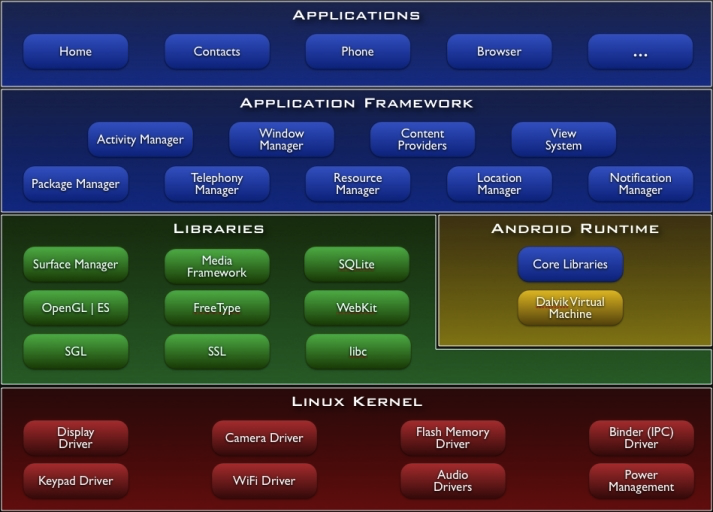
\includegraphics[scale=0.65]{system-architecture}
\begin{itemize}
\item 안드로이드에서 제공하는 기본 앱(Home, Camera, Dialer, Browser 등)과 일반 앱은 Applications 스택에 있고, Applications는 Application Framework 위에서 동작한다. 기본 앱은 소스가 공개돼 있으므로 참고 자료로 활용할 수 있다. 단말 제조사들은 일반적으로 기본 앱을 커스터마이징하고, 제조사 단말에 특화된 앱도 추가로 제공한다. 요점은 단말에 깔린 기본 앱과 우리가 만드는 앱은 동일한 레벨이라는 것이다. 다만 기본 앱은 시스템 권한을 쓸 수 있다는 게 다르다.

\item Application Framework는 자바 기반의 여러 -Manager가 있다. 내부적으로는 JNI를 연결해서 네이티브 C/C++로 작성된 것이 많다.(Telephony Manager, Location Manager 등 주로 하드웨어 관련한 것이 그렇다.) 각종 -Manager는 system\_server라는 별도 프로세스에서 실행되고, 각각 시스템 서비스 형태로 있어서 앱에서는 Context의 getSystemService(String name) 메서드로 접근해서 사용한다. 별도의 프로세스에서 실행되므로 Binder IPC를 이용한 프로세스 간 통신이 필요하다.

\item Android Runtime의 Core Libraries에는 android.jar가 있다. 여기에는 android.* 패키지, com.android.* 패키지, 자바 기본 패키지(java.*, javax.*), Apache HttpClient(마시멜로에서 제거됨), DOM/SAX/XM\-LPullParser 등 자바 클래스와 안드로이드 기본 리소스가 포함되어 있다.

\item Dalvik Virtual Machine은 자바/C/C++로 작성되어 있다(롤리팝에서는 Dalvik을 대체한 ART가 적용).\footnote{\url{https://source.android.com/devices/tech/dalvik/art.html}를 참고하자.} Register 기반의 가상 머신(Virtual Machine)으로 자바 가상 머신보다 명령이 단순하고 속도가 빠르다.
Dalvik Virtual Machine은 한 번에 여러 가상 머신 인스턴스를 띄울 수 있다. J2SE/J2EE 자바 애플리케이션을 만들다보면 여러 가상 머신 인스턴스는 당연한 얘기지만, J2ME에는 여러 Midlet이 하나의 가상 머신에서 돌아가는 방식이었고 안드로이드에서는 이 방식을 변경하였다.

\item Libraries에는 세 가지 범주의 라이브러리가 있다.\footnote{HAL(Hardware Abstraction Layer)는 별도로 나오기도 하고 Libraries에 포함하기도 한다.}
\begin{itemize}
\item Bionic이라는 커스텀 C 라이브러리(libc)\footnote{\url{http://surai.tistory.com/28}을 참고하자.}
\item WebKit/SQLite/OpenGL 같은 기능 라이브러리
\item 네이티브 시스템 서비스인 Surface Manager, Media Framework\\
/system/bin/surfaceflinger와 /system/bin/mediaserver 프로세스로 각각 실행된다.
\end{itemize}

\item 안드로이드는 리눅스 커널을 기반으로 불필요한 것은 제거하고(X-Window, glibc, 표준 리눅스 유틸리티 일부 등) 확장 패치한 것이다(Binder, Ashmem, Low Memory Killer 등).\\
이 가운데 Binder IPC는 프로세스 간 통신에 사용하는 방식이다. 
Binder에서 많이 혼동되는 게 Binder IPC(Inter Process Communication)와 Binder RPC(Remote Procedure Call)라는 두 용어인데, IPC는 하부 메커니즘이고 RPC는 IPC를 이용한 용도(리모트 콜)이다. 우리가 만드는 컴포넌트 가운데서 Service와 ContentProvider는 Binder를 통해서 다른 프로세스에서 접근할 수 있게 된다. 앱 프로세스에서 Binder Thread라는 네이티브 스레드 풀이 있고(16개까지 생성), DDMS에서 보면 Binder\_1, Binder\_2와 같은 이름의 스레드가 바로 Binder Thread에 속한 것이다. 

\end{itemize}
% 안드로이드 SDK는 Java 프로그래밍 언어를 사용하여 안드로이드 플랫폼 상의 애플리케이션 개발에 필요한 API들과 도구들을 제공한다.(kandroid)
\section{프레임워크 소스}
4.X 이상 버전은 Android SDK Manager를 이용해서 Sources for Android SDK를 선택해서 자바 소스를 다운로드할 수 있고, IDE에서 소스를 연결해서 보는 경우에 유용하다. 
2.X 버전의 소스를 확인하거나 네이티브까지 소스를 확인하려면, https://android.googlesource.com에서 관련 소스를 다운로드하면 된다.\footnote{\url{http://source.android.com/source/downloading.html}을 참고하자.} 참고로 3.X 허니콤 소스는 공개되어 있지 않다. 
3.X는 태블릿 전용 버전이고, 소스가 공개되어 이 버전이 폰에 이식된다면 파편화 문제가 심각해질 우려가 있어서 비공개로 결정되었다고 한다.
커널 소스는 \url{https://source.android.com/source/building-kernels.html}을 참고해서 별도로 다운로드한다.\\
 
프레임워크 소스를 다운로드하는 곳으로 \url{http://github.com/android}도 있는데, 여기는 읽기 전용 미러링 GitHub 계정이다. 항목별 소스 다운로드나 웹브라우저로 소스 보기에는 더 편리하다는 장점이 있다.\\

커널을 제외하고 소스 다운로드 결과는 아래와 같다.

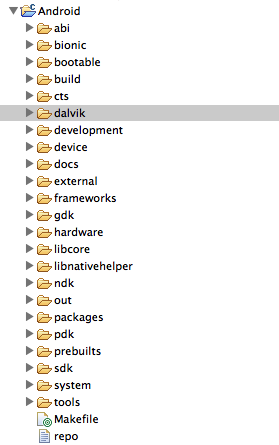
\includegraphics[scale=0.7]{sourcetree}

여기서 주요 디렉터리만 살펴보도록 하자.
\begin{itemize}
\item frameworks : 안드로이드 프레임워크. android로 시작하는 자바 패키지 포함
\item libcore: 자바 core 패키지 포함
\item system : 안드로이드 init 프로세스
\item packages : 안드로이드 기본 애플리케이션
\item bionic: 안드로이드 표준 C 라이브러리
\item dalvik: 달빅 가상 머신
\item cts: 안드로이드 호환성 테스트 관련
\item build: 빌드 시 사용
\end{itemize}

개발 시에 소스를 버전별로 모두 다운로드하지는 않고, 보통 프레임워크 소스는 
\url{http://grepcode.com}에서 확인하기도 한다. 링크가 잘 되어 있고 버전별로 차이를 확인해 볼 수도 있다.\\

개발하다가 궁금한 게 있을 때, 프레임워크 소스에서 확인하지 않고 \href{http://stackoverlow.com}{Stack Overflow}에 의존하는 경향을 가진 이들도 있다. % 면접에서 이런 분을 보기도 했다.
Stack Overflow에는 다양한 수준과 경험을 가진 사람들이 있어서 답변들이 어느 것이 맞는지 모호하기도 하고, 정작 내가 원하는 답은 없을 때도 있다.
Stack Overflow에서 답변을 찾았다고 해도 그게 맞는 것인지 검증하려면 테스트를 수행하고 프레임워크 소스로 재차 검증하는 것이 좋다.\\

예를 들어보자.
ListView의 아이템 레이아웃에 CheckBox가 있으면 ItemClick이 정상적으로 동작하지 않는다. 이런 내용은 책이나 강의에는 잘 안 나오기 때문에 처음 겪을 때 당황하게 된다. 
StackOverflow에서 검색해보면 아이템 레이아웃의 CheckBox 속성에서 android:focusable=``false''로 하라고 나온다. 이 상태에서 어쨌든 문제가 해결된다.
그런데 다른 ListView의 아이템 레이아웃에 ImageButton이 추가되었는데 또 ItemClick이 동작하지 않는다. 다시 검색을 해본다. 이런저런 얘기가 많은데 명확한 답변이 잘 안 보인다(그 가운데 물론 답이 있다). 역시 android:focusable=``false''를 써보지만 해결되지 않는다. 이때 2가지를 찾아봐야 한다. 
\begin{enumerate}
\item focusable 속성이 ListView의 OnItemClickListener에 주는 영향이 있는가? focusable 속성으로 문제가 해결되지 않으니 다른 조건이 더 있을가?
\item ImageButton의 문제가 있을까?
\end{enumerate}

먼저 ListView의 OnItemClickListener에 View의 focusable 속성이 주는 영향을 찾아보자. setOnItemClickListener() 메서드는 ListView의 상위 클래스인 AdapterView에 있다. 
여기에서 OnItemClickListener를 사용하는 위치를 찾아보면 performItemClick() 메서드이고, 또 다시 호출 위치를 따라가보면 AbsListView의 onTouchUp() 메서드에서 Child View의 hasFocusable() 리턴값이 true일 때는 클릭이 동작하지 않는 것을 볼 수 있다. Child View의 다른 조건은 보이지 않는다.\\

이제 CheckBox의 focusable 기본값은 어디에 있을까? 이 값은 style에 지정되어 있다.
CheckBox의 style은 /frameworks/base/core/res/res/values/styles.xml\footnote{<sdk>/platforms/android-XX/data/res 아래에서도 볼 수 있다.}에서 ``Widget.CompoundButton.CheckBox''를 보면 된다.\footnote{CheckBox 소스를 보면 defStyleAttr 파라미터 자리에 com.android.internal.R.attr.checkboxStyle이 있다. attrs.xml을 보면 checkboxStyle에 reference로 지정되어 있는데 다른 곳에서 정의한다는 의미이다. themes.xml에서 보면 ``@style/Widget.CompoundButton.CheckBox''로 다시 정의된 것을 볼 수 있다.}
parent를 쓰지 않고서도 속성을 상속하는 암묵적 상속이 있는데, 바로 CheckBox의 style은 ``Widget.CompoundButton'' style을 상속한다. 여기서 focusable == true로 되어있다.
따라서 레이아웃에서 CheckBox 속성을 android:focusable=``false''로 하면 style이 다시 오버라이드되어 ListView에서 정상적으로 ItemClick이 동작한다.\\

프레임워크 리소스에서 styles.xml을 보면 CheckBox, RadioButton, ToggleButton, Switch, SeekBar, EditText, ImageButton 등 위젯이 focusable == true로 되어 있다. 이런 위젯이 ListView에 포함된다면 주의해야 한다.
ListView의 각 Item View는 일반적으로 ViewGroup이고 그 안에 focusable 위젯을 가지고 있으므로 다른 방법도 가능하다. 바로 ViewGroup 레이아웃 속성에 android:descendantFocusability=``blocksDescendants''를 넣으면 된다. 이 속성은 ViewGroup의 hasFocusable() 메서드에서 체크하고 있다.\\

요점은 검색만으로 문제를 해결하고 왜 그런지를 모른다면 ListView에서 CheckBox나 ImageButton은 각각의 Tip으로만 남고 까먹기도 쉽다. 프레임워크 소스 레벨에서 검증해보면, 다음에 비슷한 문제를 맞닥뜨려도 어디서부터 문제를 찾으면 되는지 알 수 있다.\\

프레임워크 소스는 각 단말 제조사에서 커스터마이징하는 경우가 많아서 예외 스택의 라인 번호가 차이가 있어 스택을 가지고 문제 위치를 쉽게 찾지 못한다. 이 때문에 프레임워크 소스를 그대로 사용하는 레퍼런스 폰인 Nexus 시리즈를 개발에 활용하는 것은 많은 도움이 된다. 앱 프로세스 내부에서 실행되는 클래스에 대해서는 디버깅 모드에서 Breakpoint를 잡아서 값을 확인할 수 있다.\\

안드로이드 내부 구조를 다 파헤쳐볼 것도 아닌데, 전체 프레임워크 소스를 다운로드할 필요가 있을까 싶다. 필자의 경우에도 다운로드하는 걸 망설였지만, 다운로드하고서 많은 도움이 되었다. C/C++ 소스까지 깊이 이해하지는 않아도 대략이라도 내부 구조를 알 수 있고, 특히 앱의 크래시 문제를 해결하는 데 쓸모가 있다. 
안드로이드 동작 방식에 대한 이해와 경험으로 문제를 크래시를 해결하는 경우가 많지만, 실제 개발에서 크래시가 코어 자바 쪽에서 생기는 경우도 있다.
아래와 같은 에러를 보게 된다면 원인을 어떻게 찾을 것인가. 두 번째 에러는 현장에서 수많은 크래시를 발생시킨 것이다.
\begin{lstlisting}[frame=single]
Caused by: java.lang.NullPointerException
	at java.text.SimpleDateFormat.parse(SimpleDateFormat.java:1004)
	at java.text.DateFormat.parse(DateFormat.java:624)
	....
\end{lstlisting}

\begin{lstlisting}[frame=single]
Caused by: java.lang.ArrayIndexOutOfBoundsException: length=2; index=2
	at java.util.regex.Matcher.group(Matcher.java:358)
	at java.util.regex.Matcher.appendEvaluated(Matcher.java:138)
	at java.util.regex.Matcher.appendReplacement(Matcher.java:111)
	at java.util.regex.Matcher.replaceFirst(Matcher.java:304)
	at java.lang.String.replaceFirst(String.java:1793)
	....
\end{lstlisting}

안드로이드에서 사용하는 코어 자바 라이브러리는 JDK에서 자바 소스를 찾으면 안 된다. 
코어 자바 라이브러리는 Apache Harmony를 기반으로 만든 것이다.\footnote{안드로이드 N에서는 Open JDK 기반으로 변경된다고 한다} 2011년도에 Apache Harmony는 종료되었지만 안드로이드에서는 이후에도 조금씩 업데이트하고 있다. 
코어 자바 소스는 /libcore/luni/src/main/java 디렉터리 아래에서 찾고 해당 라인 위치에서 원인을 찾아서 해결해야 한다.  
libcore는 기반이 되는 자바 버전이 바뀌기 전에는 거의 변경되지 않으므로, 한 버전을 다운로드해서 여러 버전에서 참고해볼 수 있다. 프로요까지 자바5, 킷캣까지는 자바6, 현재 최신 버전은 자바7 기반이다.

\section{안드로이드 버전}
안드로이드는 버전에 따라 차이가 많기 때문에, 내용 설명에서 안드로이드 버전을 가지고 얘기하는 경우가 많다. 
표로 먼저 정리해놓고 내용에서 참고하도록 하자. 표에서는 굳이 본문에서 언급되지 않는 하위 버전은 제외하였다.\\

\begin{tabular}{|c|c|c|}\hline
코드네임 & API 레벨 & 안드로이드 버전 \\ \hline
프로요 & 8 & 2.2 \\ \hline
진저브레드 & 9 & 2.2\\ \cline{2-3}
 & 10 & 2.3\\ \hline
허니콤 & 11 & 3.0\\ \cline{2-3}
 & 12 & 3.1\\ \cline{2-3}
 & 13 & 3.2\\ \hline
ICS(아이스크림 샌드위치) & 14 & 4.0-4.0.2\\ \cline{2-3}
 & 15 & 4.0.3-4.0.4\\ \hline 
젤리빈 & 16 & 4.1\\ \cline{2-3}
 & 17 & 4.2\\ \cline{2-3}
 & 18 & 4.3\\ \hline
킷캣 & 19 & 4.4-4.4.2\\ \cline{2-3}
 & 20 & 4.4.3-4.4.4\\ \hline  
롤리팝 & 21 & 5.0\\ \cline{2-3}
 & 22 & 5.1\\ \hline 
마시멜로 & 23 & 6.0\\ \hline 
\end{tabular}\\

코드네임과 API 레벨이 일대일 매핑되지 않고, API 레벨과 안드로이드 버전도 마찬가지로 매핑되지 않아서 혼동되는 경우도 많다. 안드로이드 버전의 앞자리 숫자가 바뀌는 변화가 있는 11(허니콤), 14(ICS), 21(롤리팝), 23(마시멜로)는 기억하도록 하자.
이 책에서는 설명에서 주로 코드네임으로 언급하고, 한 코드네임 안에서 여러 API 레벨이 있는 경우 구분이 필요할 때 API 레벨까지 언급하기로 한다. 
여러 API 레벨이 있는데 코드네임만 언급하는 경우는 가장 낮은 API 레벨부터 해당하는 경우이다. 이를테면 허니콤이라고 하면 API 레벨 11 안드로이드 3.0을 얘기한다.\\

각 버전의 히스토리를 알기 위해서는 아래 링크를 보자.
\begin{itemize}
\item \url{https://en.wikipedia.org/wiki/Android_version_history}
\item \url{http://socialcompare.com/en/comparison/android-versions-comparison}
\end{itemize}
아래와 같이 공식적인 링크가 있지만 최신 버전 위주로 정리되어 있고 한 번에 보기에 편하지 않다.
\begin{itemize}
\item \url{https://www.android.com/history/}
\item \url{http://developer.android.com/intl/ko/about/dashboards/index.html}
\end{itemize}

\subsection{호환성 모드}
앱이 동작하는 안드로이드 버전을 지정하기 위해서는 AndroidManifest.xml에서 uses-sdk 항목에  android:min\-SdkVersion과 android:targetSdkVersion에 버전을 기재한다. 
만든 지 오래된 앱에서 minSdkVersion만 지정하고 targetSdkVersion을 지정하지 않은 채로 있는 것을 본 적이 있는데, targetSdkVersion를 명시하지 않으면 minSdkVersion와 동일한 값으로 지정된다.
targetSdkVersion는 반드시 지정하도록 하자. 해당 버전까지는 테스트해봤는데 앱 실행에 문제가 없다는 의미이고, 그 버전까지는 호환성 모드를 쓰지 않겠다는 뜻이다.\\

호환성 모드는 안드로이드 버전이 올라가더라도 앱의 기존 동작이 바뀌는 것을 방지하기 위한 것이다.
프레임워크 소스를 보면 targetSdkVersion을 가지고 체크하는 부분이 있다.
\footnote{\url{http://androidxref.com}에서 버전을 선택하고 Symbol에서 targetSdkVersion을 쓰고 검색하면 확인할 수 있다.}\\

버전에 따라서 기존 동작이 변경되고 호환성 모드로 동작하는 건 어떤 게 있을까? 몇 가지 예를 들어보자.
\begin{itemize}
\item AsyncTask에서 태스크를 실행하면 허니콤 이후로 병렬 실행이 아닌 순차 실행으로 변경되었다. 이것도 targetSdkVersion이 10이하이면 안드로이드 버전이 4.X 대라고 해도 기존과 동일하게 병렬 실행으로 동작한다. ScrollView, ListView나  ViewPager에서 현재 화면의 데이터를 가져올 때 AsyncTask를 통해서 가져온다면, 순차 실행으로는 적합하지 않다. 이때는  AsyncTask를 사용하지 않고 관련한 용도의 다른 라이브러리(네트워크 용도라면 Volley 등)를 사용하거나, AsyncTask를 버전에 따라 다르게 동작하도록 코드를 작성해야 한다.\\

아래는 support-v4에 포함된 AsyncTaskCompat을 간략히 한 것이다.
\begin{lstlisting}[frame=single]
	public static <Params, Progress, Result> AsyncTask<Params,
			Progress, Result> executeParallel(
            AsyncTask<Params, Progress, Result> task, Params... params) {
        if (task == null) {
            throw new IllegalArgumentException("task can not be null");
        }
        if (Build.VERSION.SDK_INT >= 11) {
            task.executeOnExecutor(AsyncTask.THREAD_POOL_EXECUTOR, params);
        } else {
            task.execute(params);
        }
        return task;
    }
\end{lstlisting}
모든 버전에서 병렬 실행을 위해서 별도 메서드를 만든 적이 있었는데, AsyncTaskCompat을 바로 사용하면 된다.

\item 메인 스레드 상에서 네트워크 통신이 진저브레드 API 레벨 9까지는 허용되었으나, 그 이후에는 에러를 발생시킨다. targetSdkVersion을 높여서 NetworkOnMainThreadException이 발생한다면, 스레드에서 네트워크 통신을 하도록 변경해야 한다.
\item 하드웨어 가속(Hardware Acceleration)은 View에서 Canvas에 그리는 모든 작업을 GPU를 가지고 하는 것이다. 하드웨어 가속은 허니콤에서 처음 시작되었고 targetSdkVersion 14 이상에서는 디폴트 옵션이다. 하드웨어 가속을 사용할 때 눈에 띄는 속도 향상은 SlidingPaneLayout이나 여러 Sliding Menu 라이브러리에서 애니메이션 시 끊김 현상이 없다는 것이다. 
필자의 경우도 애니메이션 끊김 현상이 단지 하드웨어 가속만으로 해결되는 경우를 여러 번 겪었다.
그래서 가능하면 하드웨어 가속을 쓰는 게 좋지만 항상 속도가 향상되는 것은 아니다. \url{http://developer.android.com/intl/ko/guide/topics/graphics/hardware-accel.html}을 참고해서 테스트하고 수준별(Application, Activity, Window, View)로 오버라이드하는 방법을 사용하자.
\item targetSdkVersion 14 이상에서는 App Widget에서 기본 패딩이 존재한다. 기존에는 셀의 사이즈를 꽉 채웠지만 targetSdkVersion이 올라가면 기본 패딩 때문에 App Widget의 실제 사이즈는 기존보다 작아진다. 관련해서 \ref{subsubsec:icspadding}절에 좀 더 상세하게 설명하였다.
\item targetSdkVersion 21 이상에서는 startService()나 bindService()를 실행할 때 명시적 인텐트를 사용해야 한다.
\end{itemize}


결론적으로 단말 버전에 따라 최신 기능을 쓸 수 있기 때문에 targetSdkVersion은 높여서 쓰는 것이 권장된다. 다만 targetSdkVersion을 높일 때는 테스트할 내용이 많다.

\begin{comment}
시스템의 DPI가 낮게 변경되는 건, 안드로이드가 대화면 장치(xlargeScreens)에서 
minSdkVersion이 낮은 앱을 호환성 모드로 실행하기 때문이라고 합니다.
  
\

이해하려고 읽는 김에 Best Practice - Screen Compatibility Mode를 정리하다가, 후반엔 듬성듬성 번역해 봤습니다.
http://developer.android.com/guide/practices/screen-compat-mode.html 
 
 
Screen Compatibility Mode

 
* 안드로이드 3.0 이전에 개발된 앱이 고dpi, 고dp 화면에서 너무 작게 보이는 현상을 방지하기 위한 모드.

호환모드 상태일 때:

호환모드를 사용하지 않을 때:


버전 1.6 부터 안드로이드는 다양한 화면 사이즈를 지원했다.
하지만, 앱이 Supporting Multiple Screens의 가이드를 잘 따르지 않았다면, 대형 화면에서 문제가 발생할 수 있다.
문제를 겪는 앱을 위해, 화면 호환성 모드가 개발되었다.

호환성 모드에는 2가지 버전이 존재한다.

Version 1 (Android 1.6 - 3.1)
(설명 있는데 번역하기 귀찮. 되게 옛날 얘기인듯.)
이 버전의 호환성 모드를 끄기 위해서는, android:minSdkVersion 혹은 android:targetSdkVersion이 4 이상으로 되어 있거나, android:resizable이 true로 되어 있어야 한다.

Version 2 (Android 3.2 and greater)
시스템은 어플리케이션의 레이아웃을 normal size handset (약 320dp x 480dp screen)  으로 그리고 이미지를 뻥튀기해 (scale up) 화면을 채운다.
기본적으로 레이아웃에 줌인 해서 크게 보는 것과 같다. 계단 현상이 발생한다.

이 기능은 안드로이드 3.2에서 최신 태블릿 디바이스에서 Supporting Multiple Screens의 기법들을 아직 도입하지 않은 어플리케이션들을 더  잘 지원하기 위해 도입되었다.

일반적으로, 안드로이드 3.2 이상 탑재한 대화면 디바이스에서는 어플리케이션 manifest에 명시적으로 대화면 지원이 선언되어 있지 않아도사용자가 화면 호환성 모드를 활성화 할 수 있다.
(중략)



개발자는 자신의 어플리케이션이 화면 호환성 모드를 사용할지를 제어할 수 있다. 
이하의 방법은 안드로이드 3.2 이상에서 사용 화면 호환성 모드를 활성화/비활성화 하는 방법이다.


화면 호환성 모드 끄기
안드로이드 3.0 이하를 버전을 대상으로 어플리케이션을 개발했지만, 어플리케이션이 태블릿과 같은 대화면 디바이스에서도 적절하게 리사이즈 되도록 만들었을 경우, 사용자 경험을 최상으로 유지하기 위해서는 화면 호환성 모드를 꺼야 한다.

기본적으로, 다음 중 하나의 조건이 참이면 화면 호환 모드를 사용자가 선택할 수 있게 된다.

* android:minSdkVersion, android:targetSdkVersion가 모두 10 이하이면서 <support-screens> 엘리먼트로 대화면 지원을 명시적으로 선언하지 않은 경우.
* android:minSdkVersion, android:targetSdkVersion가 모두 11 이상이면서 <support-screens> 엘리먼트로 대화면이 지원되지 않음을 명시적으로 선언한 경우.


사용자가 화면 호환성 모드를 선택할 수 없도록 하려면 다음과 같이 해야 한다.
* 가장 쉬운 방법:
<supports-screens> 엘리먼트에 android:xlargeScreens 속성을 true로 준다.
이게 전부다. 이 선언은 어플리케이션이 모든 대화면 사이즈를 지원하기 때문에, 시스템이 레이아웃을 화면에 맞춰 리사이즈한다. 이 방법은 <uses-sdk>속성에 어떤 값이 들어가 있던지 상관 없다.

* 쉽지만 다른 영향이 있는 방법:
<uses-sdk> 엘리먼트에 android:targetSdkVersion 속성을 11 이상으로 준다.
이 선언은 어플리케이션이 안드로이드 3.0을 지원하므로, 태블릿과 같은 대화면에서도 동작하도록 작성되었다는 선언이다.

주의 : 안드로이드 3.0 이상을 지정할 경우, UI에 Holographic 테마의 이펙트가 활성화되고, 액티비티에 ActionBar가 추가되고, 시스템 바의 OptionsMenu 버튼이 사라진다.


만약 위 변경을 적용한 뒤에도 화면 호환성 모드가 나타나면, manifest의 <support-screens>에 false로 선언된 속성이 없는지 확인해 봐야 한다. 가장 좋은 실천법은 지원하는 화면 사이즈를 <supports-screens> 엘리먼트를 이용해 항상 명시적으로 선언하는 것이므로, 여하간이 엘리먼트를 사용하는 게 좋다.
\end{comment}

\subsection{버전 체크}
앱에 들어가는 기능을 정할 때는 버전별 히스토리는 의미가 있지만, 앱 개발 시에 버전 관련한 주요 관심은 ``특정 클래스와 메서드가 이 버전에서 쓸 수 있는가''이다.
런타임에 해당 단말 버전에서 사용하지 않는 클래스와 메서드가 호출된다면 크래시가 발생하므로, 앞의 AsyncTaskCompat과 같이 if 문을 사용해서 버전 체크를 하는 코드를 사용한다.\\

별 게 아닌 것 같지만 앱을 배포하고서 많은 크래시를 유발하는 게 이 부분이다.
\footnote{필자의 경우도 버전 문제로 다량의 크래시를 유발했던 것을 고백하지 않을 수 없다.}
모든 안드로이드 버전의 단말을 가지고 앱의 모든 기능을 테스트하는 게 아니기 때문에, if 문으로 분기하지 않거나 비교 레벨을 잘못 기재한 경우에 실제 사용자 단말에서 사용될 때 크래시가 발생한다. 이때 즉시 문제를 수정해서 앱을 패치해보지만 이미 발생한 수많은 크래시는 어쩔 수 없다.\\

예를 들어보자. SharedPreferences.Editor에는 데이터를 반영하는 용도의 apply() 메서드와 commit() 메서드가 있다. 그런데 commit() 메서드는 XML 파일에 동기 반영이고 apply 메서드는 비동기 반영이라서 apply() 메서드를 쓰는 것이 권장된다. 그런데 apply() 메서드는 API 레벨 9부터 사용 가능하다. 속도 향상을 위해서 개선된 버전의 메서드를 사용하는 것은 당연하므로 아래와 같이 코드를 작성하도록 하자.
\begin{lstlisting}[frame=single]
	public static apply(SharedPreferences.Editor editor) {
		if (Build.VERSION.SDK_INT >= 9) {
   			editor.apply();
   		} else {
   			editor.commit();
   		}
	}
\end{lstlisting}

그런데 이런 버전 관련 분기 코드가 여기저기 다른 패키지에 산재해있는 것도 문제이다. 코드 리뷰 시에 문제점을 금방 발견하기 어렵기도 해서 compat 패키지 같은 것을 만들고 이 안에서 기능 단위로 클래스를 만드는 것을 권장한다.\\

한편 support-v4에는 이미 많은 -Compat 클래스가 있다. ViewCompat, ActivityCompat, WindowCompat, NotificationCompat, AsyncTaskCompat 등이 있고, 앞에서 작성했던 코드를 불필요하게 만드는 SharedPreferencesCompat.EditorCompat까지도 있다.(SharedPreferencesCompat.EditorCompat.apply(editor)와 같이 사용하면 된다.)\\

ScrollView에서 스크롤하다가 멈추면 스크롤 위치를 보정하는 기능을 만든 적이 있다. 그런데 이 기능이 진저브레드 이상에 있는 OverScroll 모드와 충돌하는 문제가 생겼다.
마지막까지 스크롤해서 OverScroll이 된다면 계속 떨면서 위아래로 왔다갔다 하는 현상이 생기는데 이 문제를 해결하기 위해서 처음에는 아래와 같이 코드를 작성하였다.
\begin{lstlisting}[frame=single]
	if (Build.VERSION.SDK_INT >= 9) {
   		listview.setOverScrollMode(View.OVER_SCROLL_NEVER);
	}
\end{lstlisting}
ViewCompat을 쓰면 간단하다.
\begin{lstlisting}[frame=single]
	ViewCompat.setOverScrollMode(listView, ViewCompat.OVER_SCROLL_NEVER);
\end{lstlisting}
ViewCompat.OVER\_SCROLL\_NEVER 상수처럼 -Compat에는 상위 버전에 있는 여러 상수값이 동일하게 선언되어 있는 경우가 많다.\\

support-v4에 호환 메서드가 이미 있다면 이것을 먼저 사용하고 없을 때에만 별도로 작성하자.
버전마다 동작이 다르게 코드를 작성할 때는 ViewCompat 구조를 활용하는 것도 좋다. ViewCompat의 일부 소스를 보자. 
\begin{lstlisting}[frame=single]
public class ViewCompat {
   
    public static final int OVER_SCROLL_ALWAYS = 0;

    public static final int OVER_SCROLL_IF_CONTENT_SCROLLS = 1;

    public static final int OVER_SCROLL_NEVER = 2;
    
    ...
    
    interface ViewCompatImpl { //(1)
        public boolean canScrollHorizontally(View v, int direction);
        public boolean canScrollVertically(View v, int direction);
        public int getOverScrollMode(View v);
        public void setOverScrollMode(View v, int mode);
        ...
    }

    static class BaseViewCompatImpl implements ViewCompatImpl { // (2)
        public boolean canScrollHorizontally(View v, int direction) {
            return false;
        }
        public boolean canScrollVertically(View v, int direction) {
            return false;
        }
        public int getOverScrollMode(View v) {
            return OVER_SCROLL_NEVER;
        }
        public void setOverScrollMode(View v, int mode) {
            // Do nothing; API doesn't exist
        }
        ...
    }

    static class EclairMr1ViewCompatImpl extends BaseViewCompatImpl { // (3)
        ...
    }

    static class GBViewCompatImpl extends EclairMr1ViewCompatImpl { // (4)
        @Override
        public int getOverScrollMode(View v) {
            return ViewCompatGingerbread.getOverScrollMode(v); // (5)
        }
        @Override
        public void setOverScrollMode(View v, int mode) {
            ViewCompatGingerbread.setOverScrollMode(v, mode); // (6)
        }
    }

    static class HCViewCompatImpl extends GBViewCompatImpl {
      	...
    }

    static class ICSViewCompatImpl extends HCViewCompatImpl {
        @Override
        public boolean canScrollHorizontally(View v, int direction) {
            return ViewCompatICS.canScrollHorizontally(v, direction);
        }
        @Override
        public boolean canScrollVertically(View v, int direction) {
            return ViewCompatICS.canScrollVertically(v, direction);
        }
        ...
    }

    static class JBViewCompatImpl extends ICSViewCompatImpl {
        ...
    }

    static class JbMr1ViewCompatImpl extends JBViewCompatImpl {
    	...
    }

    static class KitKatViewCompatImpl extends JbMr1ViewCompatImpl {
        ...
    }

    static final ViewCompatImpl IMPL;
    static { // (7)
        final int version = android.os.Build.VERSION.SDK_INT;
        if (version >= 19) {
            IMPL = new KitKatViewCompatImpl();
        } else if (version >= 17) {
            IMPL = new JbMr1ViewCompatImpl();
        } else if (version >= 16) {
            IMPL = new JBViewCompatImpl();
        } else if (version >= 14) {
            IMPL = new ICSViewCompatImpl();
        } else if (version >= 11) {
            IMPL = new HCViewCompatImpl();
        } else if (version >= 9) {
            IMPL = new GBViewCompatImpl();
        } else {
            IMPL = new BaseViewCompatImpl();
        }
    }

    public static boolean canScrollHorizontally(View v, int direction) {
        return IMPL.canScrollHorizontally(v, direction);
    }

    public static boolean canScrollVertically(View v, int direction) { // (8)
        return IMPL.canScrollVertically(v, direction);
    }

    public static int getOverScrollMode(View v) {
        return IMPL.getOverScrollMode(v);
    }

    public static void setOverScrollMode(View v, int overScrollMode) {
        IMPL.setOverScrollMode(v, overScrollMode);
    }

 	...
}

\end{lstlisting}
\begin{itemize}
\item 11라인(1)의 ViewCompatImpl 인터페이스에는 Compat에서 사용하려는 메서드 목록이 들어간다. 
\item 79라인(7)의 정적 초기화 블록에서 버전에 따라 인터페이스 구현체가 IMPL 변수에 들어간다.
\item 19라인(2)에 기본 구현체가 있고 35라인(3) 이후 각 버전의 구현체는 낮은 버전의 구현체를 상속하고 변경되는 내용은 오버라이드한다.
\item OverScrollMode 관련한 메서드는 진저브레드부터 있으므로 39라인(4)의 GBViewCompatImpl에서 getOverScrollMode와 setOverScrollMode를 오버라이드하는 것을 볼 수 있다.
\item 102라인(8)부터 있는 정적 메서드는 결과적으로 버전에 매핑돼 있는 구현체의 메서드를 호출한다.
\end{itemize}

ViewCompat의 42라인(5), 46라인(6)에서 사용하는 ViewCompatGingerbread은 package private 클래스이다.
\begin{lstlisting}[frame=single]
class ViewCompatGingerbread {
    public static int getOverScrollMode(View v) {
        return v.getOverScrollMode();
    }

    public static void setOverScrollMode(View v, int mode) {
        v.setOverScrollMode(mode);
    }
}
\end{lstlisting}

\begin{comment}
이를테면 ArrayAdapter의 addAll 메서드 같은 게 API 레벨 11부터 있다.
 

ClipBoardManager는 2개가 있다.

http://developer.android.com/intl/ko/reference/android/os/Build.VERSION\_CODES.html
\end{comment}

\chapter{메인 스레드와 Handler}
메인 스레드에서 UI 이벤트를 처리하는 메커니즘을 살펴보자. Handler는 메인 Looper와 연결되어 메인 스레드에서 Message를 처리하는 중심 역할을 한다. Handler는 백그라운드 스레드에서도 특별한 용도로 사용 가능하다는 점에서 다음 장의 백그라운드 스레드와도 내용이 연결된다.

\section{메인 스레드}
애플리케이션 동작은 당연히 멀티 스레드이지만, UI를 업데이트하는 데는 단일 스레드 모델(Single Thread Model: 해당 변수나 메서드를 사용하는 시점에는 하나의 스레드만 실행)이 적용된다.\footnote{롤리팝에서는 Render Thread가 추가되어 offload atomic animation을 실행한다}
멀티 스레드로 UI를 업데이트하면 동일한 UI 자원을 사용 시 교착 상태(deadlock), 경합 상태(race condition) 등 여러 문제가 발생하기 때문에 메인 스레드에서만 UI 업데이트를 허용하고 있다.\\
% 싱글 스레드 이벤트 큐 모델

\begin{comment}
\colorbox{tearose}{\parbox[t]{15cm}{
스레드 A가 특정 lock을 잡고 있으면 그 lock을 확보해야 하는 다른 스레드 B에서는 대기해야 한다. 그런데 B에서는 A에서 추가로 확보하려고 하는 lock을 이미 잡고 있다면, 서로 lock이 풀릴 때까지 계속 대기할 수 밖에 없다. 이것이 교착 상태이다. 
예를 들어 화면에 성과 이름을 입력하려는 A, B 두 스레드가 있다. 
두 스레드는 자신이 입력한 것이 바로 덮어 쓰여지는 것이 싫고, 온전히 이름을 다 입력하고자 한다. 
그래서 한국인 이름을 입력하는 A 스레드에서는 다른 스레드가 접근 못하도록 lock을 잡고서 입력하고서, 그 다음에 이름을 입력하려고 한다.
외국인 이름을 입력하는 스레드에서는 이름에 접근하면서 lock을 잡고, 그 다음에 성에 접근하려고 한다. 이 때 두 스레드는 어느 시점에 교착 상태에 이르게 된다. 교착 상태는 일반적으로 lock을 잡는 순서를 일정하게 하면 해결되지만, 복잡한 프로그램에서 이 순서를 맞추는 게 간단치 않고 성능에 나쁜 영향을 줄 수도 있다.\footnote{\url{https://ko.wikipedia.org/wiki/교착_상태}를 참고하자.}\\
경합 상태는 2개 이상의 스레드에서 공유 데이터에 접근해서 동시에 변경하려 할 때 발생한다. 스레드 실행은 내부적으로 스레드 스케줄링 알고리즘에 따르기 때문에, 스레드끼리 어느 것이 먼저 공유 데이터에 접근할지 순서는 알 수 없고 스레드끼리 경주(racing)하는 상황이 생긴다.\\

러브 액츄얼리라는 영화에서 많이 기억되는 장면이 있는데, 사랑하는 상대방한테 남자가 창밖에서 종이를 한 장씩 넘기며 고백하는 장면이다.
비유하자면 이것이 바로 안드로이드에서 UI를 업데이트 하는 방식이다. 상대방에게 보여주는 종이가 바로 UI 화면이라고 보면 된다. 종이가 스케치북으로 되어 있어 순서대로 넘기는 것은 일종의 순서를 보장하는 큐라고 할 수 있다. 그리고 종이를 넘기는 남자는 메인 스레드에 해당한다.
만일 남자(메인 스레드)가 혼자서 종이를 넘기지 않고, 다른 사람(스레드)에게 종이를 상대방이 보는 화면 앞으로 종이를 가져오라고 하면, 어떤 일이 벌어질까? 바로 이 상황이 경합 상태이다. 종이의 순서를 보장할 수 없으니 사랑 고백이 엉뚱한 얘기가 될 수도 있고, 어느 종이는 순식간에 다른 종이로 바뀔 테니, 상대방이 못 보는 메시지도 생겨난다.
}}\newline\newline
\end{comment}

앱이 시작되면서 메인 스레드가 생성된다. 컴포넌트는(Activity, Service, BroadcastReceiver, Application) 메인 스레드에서 시작되고 그 안의 메서드 호출은 기본적으로 메인 스레드에서 실행된다. 
메인 스레드는 UI를 변경할 수 있는 유일한 방법이기 때문에 메인 스레드를 UI 스레드라고 부르기도 한다. 
Service, BroadcastReceiver, Application은 직접적으로 UI는 아니기 때문에, UI 스레드라는 것은 메인 스레드의 한 부분만을 얘기하는 것이지만 이해를 위해 많이 사용된다.\\

일반적인 자바 애플리케이션에서는 main() 메서드로 실행되는 것이 바로 메인 스레드이다.
\begin{lstlisting}[frame=single] 
public class Hello {

	public static void main(String[] args) {
		System.out.print("Hello");
	}

}
\end{lstlisting}

안드로이드 애플리케이션의 메인 스레드는 뭔가 다른 특별한 것일까? 그렇지 않다. 
안드로이드 프레임워크 내부 클래스인 android.app.ActivityThread가 바로 애플리케이션의 메인 클래스\footnote{실제로는 ZygoteInit이 시작점이지만 우리가 이해해야 하는 지점은 ActivityThread부터이다.}이고, ActivityThread의 main() 메서드가 애플리케이션의 시작 지점이다.\newpage

\begin{lstlisting}[frame=single, caption=ActivityThread.java] 
	public static void main(String[] args) {
		SamplingProfilerIntegration.start();

		CloseGuard.setEnabled(false);

		Environment.initForCurrentUser();

		EventLogger.setReporter(new EventLoggingReporter());

		Process.setArgV0("<pre-initialized>");

		Looper.prepareMainLooper();

		ActivityThread thread = new ActivityThread();
		thread.attach(false);

		if (sMainThreadHandler == null) {
			sMainThreadHandler = thread.getHandler();
		}

		AsyncTask.init();

		if (false) {
			Looper.myLooper().setMessageLogging(
					new LogPrinter(Log.DEBUG, "ActivityThread"));
		}

		Looper.loop(); // (1)

		throw new RuntimeException("Main thread loop unexpectedly exited");
	}
\end{lstlisting}

여기서 제일 중요한 곳은 28라인(1)이다. 
Looper.loop() 메서드에는 무한 반복문이 있어서 main() 메서드는 프로세스가 종료될 때까지 끝나지 않는다.
ActivityThread는 클래스명 때문에 Thread를 상속한 게 아닐까 하는 오해를 받기도 하지만 전혀 그렇지 않다.
게다가 Activity만 관련돼 있는 것도 아니고 모든 컴포넌트들이 다 관련돼 있다.

%http://warmz.tistory.com/588
% http://www.myexception.cn/android/1710667.html
% http://www.2cto.com/kf/201407/317129.html

\section{Looper}
Looper 클래스\footnote{\url{http://developer.android.com/reference/android/os/Looper.html}}는 내용이 단순하다. Looper에서 필요한 내용을 알아보자.
\begin{itemize}
\item TLS(Thread Local Storage)에 Looper를 저장한다. 구체적으로 ThreadLocal<Looper>에 set() 메서드로 새로운 Looper를 추가하고 get() 메서드로 Looper를 가져오는데, 각 스레드별로 다른 Looper가 반환된다.
Looper.prepare()를 통해 스레드별로 Looper를 생성하는데, 특히 메인 스레드의 Looper는 ActivityThread에서 Looper.prepareMainLooper()를 통해서 생성되고, Looper.getMainLooper()를 통해서 어디서든 가져올 수 있다.
\item Looper별로 MessageQueue를 가진다. 특히 메인 스레드에서는 이 MessageQueue를 통해서 UI 작업에서 경합 상태를 해결한다. 
개발 중에 Queue 구조가 필요할 때 java.util.Queue의 여러 구현체를 사용할 수도 있지만 Looper 사용도 고려해보자. 특히 스레드별로 다른 Queue를 사용할 때는 Looper를 사용하는 게 더 단순해질 수 있다(결론적으로는 Handler를 사용하는 것이다).
\end{itemize}

Looper.loop() 메서드의 주요 코드를 보자.
\begin{lstlisting}[frame=single, caption=Looper.java] 
	public static void loop() {
		final Looper me = myLooper();
		if (me == null) {
			throw new RuntimeException(
					"No Looper; Looper.prepare() wasn't called on this thread.");
		}
		final MessageQueue queue = me.mQueue;
		for (;;) {
			Message msg = queue.next(); // (1)
			if (msg == null) {
				return; // (2)
			}
			msg.target.dispatchMessage(msg); // (3)
			msg.recycle();
		}
	}
	
	public void quit() {
        mQueue.quit(false);
    }
    
    public void quitSafely() {
        mQueue.quit(true);
    }
\end{lstlisting}	
\begin{itemize}
\item 13라인(3)이 바로 메시지를 처리하는 부분이다. 
for 루프를 돌면서 MessageQueue에서 다음 Message를 꺼내서 13라인(3)에서 dispatchMessage()를 호출한다. 
\item quit(), quitSafely() 메서드는 Looper를 종료한다. 구체적으로 MessageQueue의 quit() 메서드에 boolean 값을 전달하고, 9라인(1)의 queue.next()에서 null을 리턴하고 11라인(2)에서 for 루프가 종료된다.
Looper API 문서에서 quit()과 quitSafely() 메서드 차이를 보도록 하자.
quit() 메서드는 아직 처리되지 않은 Message는 모두 제거한다.
quitSafely() 메서드는 sendMessageDelayed() 등을 써서 실행 시간을 뒤로 미룬 경우에 해당하는 것으로, quitSafely() 메서드를 실행하는 시점에 현재 시간보다 뒤쪽에 있는 Message를 제거하고 그 앞쪽에 있는 Message는 계속해서 처리를 진행한다. 다만 quitSafely() 메서드는 젤리빈 API 레벨 18 이상에서 쓸 수 있다.\\
\end{itemize}

\section{Message와 MessageQueue}
\label{sec:messagequeue}
MessageQueue는 Message를 담고 있는 자료구조이다.
MessageQueue의 구조는 ArrayBlockingQueue보다는 LinkedBlockingQueue에 가깝다. ArrayBlockingQueue는 배열에 노드를 추가하는 방식이지만, LinkedBlockingQueue는 다음 노드에 대한 링크를 변수로 가진다. 
Array 구조에 비해서 Link 구조는 일반적으로 개수의 한계가 없고 삽입 속도가 빠르다. 
대신 Array 구조는 랜덤 인덱스 접근이 가능하고 Link 구조는 순차 접근을 해야 한다. MessageQueue는 실행하기로 한 시간 순으로 삽입되어서 빠른 것부터 순차적으로 꺼내어진다.\\

먼저 Message 클래스를 보자.
\begin{lstlisting}[frame=single, caption=Message.java] 
public final class Message implements Parcelable {

	public int what;

	public int arg1;

	public int arg2;

	public Object obj;

	public Messenger replyTo;
	
	...

	/* package */long when;

	/* package */Bundle data;

	/* package */Handler target;

	/* package */Runnable callback;

	/* package */Message next;
	
	...
}
\end{lstlisting}
MessageQueue에 들어가는 android.os.Message에는 public 변수에 int arg1, int arg2, Object obj,
Messenger replyTo, int what 5개가 있고 Message를 만들 때 이 변수에 값을 넣는다.
Message에는 package private 변수도 여러 개 있다. android.os 패키지 아래에 Looper, Message, MessageQueue, Handler도 있는데, 이들 클래스에서 Message의 package private 변수에 직접 접근한다. target이나 callback 같은 것들이 Handler에서 postXxx(), sendXxx() 메서드를 호출할 때 Message에 담겨서 MessageQueue에 들어간다. postXxx(), sendXxx() 메서드에서 실행하려는 시간(AtTime)이 전달되고, 나중에 호출한 것이라도 AtTime이 앞서면 Queue 중간에 삽입된다. 이것이 삽입이 쉬운 Link 구조를 사용한 이유이다.\\

Message를 생성할 때는 오브젝트 풀(object pool)에서 가져오는 Message.obtain() 메서드나 Handler의 obtainMessage() 메서드를 사용하는 것을 권장한다. 내부적으로 Handler의 obtainMessage()는  Message.obtain()을 다시 호출한다.
오브젝트 풀은 Message에 정적 변수로 있고(여기서도 Link로 연결됨) 최대 50개까지 Message를 저장한다. 그리고 Looper.loop() 메서드에서 Message를 처리하고 나서 recycleUnChecked() 메서드를 통해 Message를 초기화하고 최대 개수 50개에 도달하지 않았다면 오브젝트 풀에 추가하는 형태이다.
new Message()와 같이 기본 생성자를 가지고서 값을 채워도 동작에는 문제가 없어 보이지만, Message 처리가 끝나면 불필요하게 풀에 추가하는 동작이 되어서 최대 개수에 이르는 건 시간 문제가 된다. 
풀에서 가져와서(여분이 없으면 새로 생성) 풀에 돌려줘야지 따로 생성해서 풀에 돌려주는 건 불필요한 자원 낭비가 된다.\footnote{Handler를 통해 Message를 처리하는 게 아니라, 파라미터에 별도 객체를 만들지 않고 Message로 대신 사용해서 주고받는 경우에만 Message 기본 생성자로 쓰도록 하자.}\\

%Handler의 removeMessages 메서드에서는 원하는 Message를 제거하기 위해 Queue를 순회하는데, 이 경우에는 Link 구조가 조금 불리해진다.

\section{Handler}
Handler는 Message를 MessageQueue에 넣는 기능과 MessageQueue에서 꺼내 처리하는 기능을 함께 제공한다. Handler와 Looper, MessageQueue의 관계, 그리고 사용 방법에 대해서 알아보자.

\subsection{Handler 생성}
Handler를 사용하려면 먼저 생성자를 이해해야 한다. 
Handler에는 기본 생성자 외에 Hanlder.Callback 또는 Looper가 전달되는 생성자들이 있다. 
\begin{itemize}
\item Handler()
\item Handler(Handler.Callback callback)
\item Handler(Looper looper)
\item Handler(Looper looper, Handler.Callback callback)
\end{itemize}
당연한 얘기지만 내부적으로 파라미터가 가장 많은 4번째 생성자를 다른 생성자에서 호출한다.
Handler는 Looper(결국 MessageQueue)와 연결되어 있는데, 이들 생성자와 어떤 관계일까? 
기본 생성자는 바로 현재 스레드의 Looper를 사용하겠다는 의미이다(Looper는 Thread Local Storage에 들어간다고 앞에서 얘기했다).
메인 스레드에서 Handler 기본 생성자가 불린다면, 앱 프로세스가 시작할 때 ActivityThread에서 메인 Looper를 생성한 것을 사용한다. 
이것이 우리가 UI 코드를 만들 때 많이 사용하는 방식이다.\\

그럼 백그라운드 스레드에서 기본 생성자를 사용한다면 어떨까? 이때는 Looper가 준비되어 있지 않다면 RuntimeException을 발생시킨다. 
``Can't create handler inside thread that has not called Looper.prepare''
이 메시지에 따르면 먼저 Looper.prepare()를 실행해서 해당 스레드에서 사용할 Looper를 준비해야 한다(내부적으로 prepare() 메서드는 MessageQueue를 생성하는 것 말고는 별 게 없다).\\

Looper API 문서를 보면 백그라운드 스레드에서 Handler를 사용하는 방법이 나온다.

\begin{lstlisting}[frame=single, caption=LooperThead, label=src:LooperThread] 
class LooperThread extends Thread {
	public Handler mHandler;

	public void run() {
		Looper.prepare();

		mHandler = new Handler() {
        	public void handleMessage(Message msg) {
            	// process incoming messages here
			}
		};

		Looper.loop();
	}
}
\end{lstlisting}
LooperThread에서 스레드를 시작하면 Looper.loop()에 무한 반복문이 있기 때문에 해당 스레드는 종료되지 않고, mHandler에서 sendXxx(), postXxx() 메서드를 사용하면 스레드 내에서 handleMessage() 메서드를 실행한다.\\

그런데 앱을 만들다 보면 가끔 위에 얘기한 RuntimeException을 만나는 경우가 있다.
예를 들어, 어떤 메서드가 단순하게 TextView의 setText()를 실행하지만, 메서드 호출을 하는 곳이 여러 군데이거나 메서드 호출 스택이 깊어서 어디서 호출하는지 금방 파악이 안되는 경우도 있다.
여러 곳에서 사용하는 메서드라면 메인 스레드뿐 아니라 백그라운드 스레드에서도 호출할 가능성이 있다. 
new Handler()로 생성하고 post() 메서드를 통해서 TextView를 변경하려 하는데, Handler 생성을 메인 스레드에서 하는지 백그라운드 스레드에서 하는지 모호한 경우가 있다.
메인 스레드라면 이미 메인 Looper가 있어서 문제가 되지 않는데, 백그라운드 스레드라면 대응하는 Looper가 당장 없을 때 RuntimeException을 만나게 된다.\\

예를 들어, 아래 코드에서는 BadgeListener의 updateBadgeCount()에서 UI를 변경한다.
\begin{lstlisting}[frame=single] 
	public void process(BadgeListener listener) {
		int count = ...
		listener.updateBadgeCount(count);
	}
\end{lstlisting}	

process() 메서드는 메인 스레드에서 호출한다면 문제가 없지만, 백그라운드 스레드에서 호출할 때 CalledFromWrongThreadException을 발생시킨다. 
이때 Looper와 Handler의 관계를 잘 모른다면 아래처럼 작성할 수 있다.
\begin{lstlisting}[frame=single] 
	public void process(BadgeListener listner) {
		int count = ...
		new Handler().post(new Runnable() {
		
			public void run() {
				listner.updateBadgeCount(count);
			}
			
		});
	}
\end{lstlisting}	
백그라운드 스레드에서는 Looper가 연결되어 있지 않다면 RuntimeException이 발생한다.
UI를 업데이트하기 때문에 백그라운드 스레드의 Looper를 생성해도 도움이 안되고, 바로 메인 Looper를 사용해야 한다. 메인 Looper와 연결된 Handler를 사용하는 것으로 Handler의 여러 생성자 가운데 세 번째 생성자를 사용하면 된다.
\begin{lstlisting}[frame=single] 
	public void process(BadgeListener listner) {
		int count = ...
		new Handler(Looper.getMainLooper()).post(new Runnable() {
		
			public void run() {
				listner.updateBadgeCount(count);
			}
			
		});
	}
\end{lstlisting}

\subsection{Handler 동작}
앞에서도 언급했듯이 Handler는 Message를 MessageQueue에 보내는 것과 Message를 처리하는 것을 함께 제공한다. post(), postAtTime(), postDelayed() 메서드를 통해서 Runnable 객체도 전달되는데, 실제로 Runnable도 내부적으로 Message에 포함되는 값이다.\\

Handler에서 Message를 보내는 메서드 목록을 살펴보자.\\

\scalebox{0.8}{
\begin{tabular}[fontsize=\tiny]{|l|l|l|} \hline
 & send & post \\ \hline
기본 & sendEmptyMessage(int what) & post(Runnable r)
\\
 & sendMessage(Message msg) & \\ \hline
Delayed & sendEmptyMessageDelayed(int what, long delayMillis) & postDelayed(Runnable r, long delayMillis)\\
 & sendMessageDelayed(Message msg, long delayMillis) & \\ \hline
AtTime & sendEmptyMessageAtTime(int what, long uptimeMillis)
 & postAtTime(Runnable r, Object token, long uptimeMillis) \\
  & sendMessageAtTime(Message msg, long uptimeMillis) & postAtTime(Runnable r, long uptimeMillis)\\ \hline
FrontOfQueue & sendMessageAtFrontOfQueue(Message msg)
 & postAtFrontOfQueue(Runnable r)
\\ \hline
\end{tabular}
}
\newline

\begin{itemize}
\item Message의 what 값만을 전달하는 sendEmptyMessage(), sendEmptyMessageDelayed(), sendEmptyMessageAtTime() 메서드가 있다.
\item -Delayed로 끝나는 메서드는 내부적으로 -AtTime 메서드를 호출한다. 현재 uptimeMillis에 delayMillis를 더한 값이 uptimeMillis 파라미터에 들어간다.
\item postAtFrontOfQueue() 메서드는 특별한 상황이 아니면 쓰지 말라는 가이드가 있다. 
권한 문제나 심각한 서버 문제처럼, 앱을 더 이상 사용할 수 없는 특별한 때가 아니면 사용할 일이 없다. 남용하면 안되는 메서드이다.
\end{itemize}

Looper.loop() 메서드에서 호출하는 Handler의 dispatchMessage() 메서드를 보자.
\begin{lstlisting}[frame=single, caption=Handler.java] 
	public void dispatchMessage(Message msg) {
		if (msg.callback != null) { // (1)
			handleCallback(msg);
		} else {
			if (mCallback != null) {
				if (mCallback.handleMessage(msg)) {
					return;
				}
			}
			handleMessage(msg);
		}
	}
	
	private static void handleCallback(Message message) {
		message.callback.run();
	}
\end{lstlisting}
dispatchMessage()는 public 메서드이다. 
드물긴 하지만 sendXxx()나 postXxx() 메서드를 쓰지 않고 직접 dispatchMessage() 메서드를 사용하기도 하는데, 이때는 MessageQueue를 거치지 않고 직접 메시지를 처리하는 것이다.
2라인(1)에서 callback Runnable이 있다면 그것을 실행하고 아니면 handleMessage()를 호출하고 있다.

\subsection{Handler 용도}
Handler는 일반적으로 UI 갱신을 위해 사용된다. 관련해서 해당 케이스를 살펴보자.
\begin{itemize}
\item 네트워크나 DB 작업 등 백그라운드 스레드 작업 중에 UI를 업데이트한다. 
AsyncTask에서도 내부적으로 Handler를 이용해서 onPostExecute() 메서드를 실행한다.

\item UI 작업 중에 다음 UI 갱신 작업을 MessageQueue에 넣어 예약한다. 작업 예약이 필요한 경우가 있다.
예를 들어, Activity의 onCreate() 메서드에서 하지 못하는 여러 가지 일들이 있다. 소프트 키보드를 띄운다든가, ListView의 setSelection() 메서드를 호출한다든가 하는 것이 onCreate() 메서드에서는 잘 동작하지 않는다. 이때 Handler를 이용해서 현재 작업이 끝난 이후에 다음 타이밍을 기다려서 진행한다.

\item 반복해서 UI를 갱신한다. DigitalClock이나 TextClock 같은 위젯도 Handler를 이용해서 현재 시간을 갱신하고 있다.
반복적인 UI 갱신 패턴은 아래와 같다.
\begin{lstlisting}[frame=single] 
  	private static final int DELAY_TIME = 2000;
	private Runnable updateTimeTask = new Runnable() {

		@Override
		public void run() {
			systemInfo.setText(monitorService.getSystemInfo());
			...
			handler.postDelayed(this, DELAY_TIME); // (1)
		}

	};
	
	public void onClickButton(View view) {
		handler.post(updateTimeTask); 
	}
\end{lstlisting}
UI 갱신이 끝나고 8라인(1)에서 postDelayed()에 Runnable 자체를 전달해서 계속 반복하게 된다.

\item 시간을 제한할 때 사용한다. 안드로이드 내부적으로 ANR을 판단할 때도 사용하는 방법이다.
아래 코드는 개발자 가이드에 있는 것인데, 블루투스 LE 디바이스를 스캔할 때 시간 제한을 둔 것이다.
\begin{lstlisting}[frame=single] 
	private static final long SCAN_PERIOD = 10000;
	...
	private void scanLeDevice(final boolean enable) {
	    if (enable) {
	    	mHandler.postDelayed(new Runnable() { // (1)
	    		
	    		@Override
	    		public void run() {
	    			mScanning = false;
	    			mBluetoothAdapter.stopLeScan(mLeScanCallback);
	    		}
	    	}, SCAN_PERIOD);
	
	    	mScanning = true;
	    	mBluetoothAdapter.startLeScan(mLeScanCallback); // (2)
	    } else {
	    	mScanning = false;
	    	mBluetoothAdapter.stopLeScan(mLeScanCallback);
	    }
	    ...
	}
\end{lstlisting}
15라인(2)에서 startLeScan()을 실행하는데, 5라인(1)의 postDelayed(Runnable) 메서드에서 10초 후에 stopLeScan()을 실행하도록 Runnable Message를 전달하였다.\\

앱에서 많이 사용하는 방식으로 몇 초 내에 Back 키를 다시 누를 때만 종료하게 할 때도 마찬가지 방식을 사용한다.
\begin{lstlisting}[frame=single] 
	private boolean isBackPressedOnce = false; // (1)
	
	@Override
	public void onBackPressed() {
		if (isBackPressedOnce) { // (2)
			super.onBackPressed();
		} else {
			Toast.makeText(this, R.string.backpressed_message,
				Toast.LENGTH_SHORT).show(); // (3)
			isBackPressedOnce = true; // (4)
			timerHandler.postDelayed(timerTask, 5000);	// (5)		
		}
	}
	
	private final Runnable timerTask = new Runnable() { // (6)
		
		@Override
		public void run() {
			isBackPressedOnce = false;
		}
		
    };
\end{lstlisting}
\begin{itemize}
\item 1라인(1)에서 isBackPressedOnce 변수가 종료 플래그이다. 최초 값은 false이다.
\item 5라인(2)에서 종료 플래그가 true이면 종료한다. 최초 값이 false이기 때문에 처음에는 이 조건에 걸리지 않는다.
\item 처음 Back 키를 누르면 9라인(3)에서 ``정말 종료하시겠습니까?''라는 토스트를 띄운다. 그리고서 10라인(4)에서 종료 플래그를 true로 바꾼다.
\item 11라인(5)에서 postDelayed() 메서드로 5초 후에 할 작업을 지정한다.
\item 15라인(6) 이하를 보면 Runnable Message는 종료 플래그를 다시 false로 되돌린다.
\end{itemize}

% 스크롤이나, 패닝 중에 쓰는 예도 필요하지 않을까?
\end{itemize}

안드로이드 프레임워크에서도 내부적으로 Handler를 많이 사용한다. 
메인 스레드에서 실행해야 하는 작업들이 Handler를 사용해서 내부적으로 메인 Looper의 MessageQueue를 통해서 순차적으로 진행된다.
\begin{itemize}
\item ActivityThread에 내부 클래스인 H는 Handler를 상속한다. 
컴포넌트 생명주기 관련해서 모두 H를 거친다. Message의 what에 해당하는 int 상수에는 LAUNCH\_ACTIVITY, RESUME\_ACTIVITY, PAUSE\_ACTIVITY, DESTROY\_ACTIVITY, CREATE\_SERVICE, STO\-P\_SERVICE, RECEIVER, BIND\_APPLICATION, EXIT\_APPLICATION 등이 있다.

\item Touch나 Redraw 등 이벤트 처리를 위한 ViewRootImpl 클래스가 있다(MSG\_INVALIDATE, MSG\_R\-E\-SIZED, MSG\_DISPATCH\_KEY, MSG\_CHECK\_FOCUS, MESSAGE\_DISPACH\_DRAG\_EV\-ENT 등).
ICS까지는 ViewRootImpl이 Handler를 상속했지만, 젤리빈부터는 내부 클래스로 ViewRootHandler를 사용한다.
ViewRootImpl에서 처음 그릴 때나 다시 그리기 필요한 경우(invalidate, 레이아웃 변경, Visibility 변경 등)는 Choreographer에 위임하는데, Choreographer에서 내부적으로 Handler를 상속한 FrameHandler를 다시 사용한다.
% Activity의 Window마다 있다.

\item Activity는 멤버 변수에 Handler가 있고 runOnUiThread() 메서드에서만 사용된다. 

\item View에는 ViewRootImpl에서 전달된 ViewRootHandler를 post()와 postDelayed() 메서드에서 사용한다.
% ViewRootImpl의 performTravers에서 ViewGroup의 dispatchAttachedToWindow() 메서드를 호출하면서 연결된다.
\end{itemize}

\subsection{타이밍 이슈}
개발하다 보면 수많은 타이밍 이슈를 접하게 된다. 원하는 시점과 실제 동작에서 차이가 생기는데, 이런 타이밍 이슈는 메인 스레드와 Handler를 이해한다면 생각보다 단순해진다.\\

Activity의 onCreate() 메서드에서 Handler의 post() 메서드를 실행하면, 실제 post() 메서드에 전달되는 Runnable이 호출되는 시점은 언제일까? onCreate() 다음일까 아니면 다른 어느 시점일까?
메인 스레드에서는 한 번에 한 작업 밖에 하지 못하고, 여러 작업이 서로 엉키지 않기 위해서 메인 Looper\footnote{Context의 getMainLooper()를 통해 가져올 수 있다.}의 MessageQueue에서 Message를 하나씩 꺼내서 처리한다는 것을 먼저 염두에 두자.
각각의 생명주기 메서드는 MessageQueue에서 각각 꺼내지면서 실행되는 것인지 의문을 가져볼 수 있다. 결과적으로 전혀 그렇지 않다.
MessageQueue에서 Message를 하나 꺼내오면 onCreate()에서 onResume()까지 쭉 실행된다.\footnote{ActivityThread의 handleLaunchActivity() 메서드를 참고하자.} 그럼 바로 답이 나온다. 
onCreate()에서 Handler의 post()에 넣은 Runnable은 onResume() 이후에 실행된다.
이미 MessageQueue에서 꺼내져서 실행 중이기 때문에 도중에 postAtFrontOfQueue() 메서드를 실행해도 마찬가지로 onResume() 이후에 실행된다.\\

%Application의 onCreate에서 Hanlder.post를 호출해도 onResume 메서드 이후에 실행되는 것을 볼 수 있다.\\
Handler는 정확한 지연 시간(delay time)을 보장하지는 않는다. MessageQueue에서 먼저 나온 Message 처리가 오래 걸린다면 실행이 당연히 늦어진다. 지연 시간과 관련한 간단한 샘플을 보자.
\begin{lstlisting}[frame=single, caption=부정확한 지연시간] 
		Handler handler = new Handler();
		handler.postDelayed(new Runnable() { // (1)

			@Override
			public void run() {
				Log.d("suribada", "200 delay");
			}
			
		}, 200);
		
		handler.post(new Runnable() { // (2)

			@Override
			public void run() {
				Log.d("suribada", "just");
				SystemClock.sleep(500);
			}
			
		});
\end{lstlisting}
2라인(1)과 11라인(2)에서 각각 Runnable Message를 보냈다. 2라인(1)에서 첫 번째 메시지는 먼저 보냈지만 200ms 이후에 실행되는 것이고, 11라인(2)에서 보낸 두 번째 Message는 즉시 실행되지만 sleep() 시간을 포함하여 500ms가 걸리는 작업이 되었다. 
단일 스레드의 규칙 때문에 먼저 처리해야 하는 것을 다 끝내야만, 뒤의 것을 처리할 수 있다. ``200 delay''라는 로그는 따라서 200ms가 아닌 최소 500ms 이후에 남게 된다.
결론적으로 지정한 지연 시간이 지나고서 정확히 실행된다고 가정하면 안된다. 예처럼 200ms 간격을 두었다면 그 사이에 여러 Message가 MessageQueue에 쌓일 가능성이 있다(Activity를 시작하거나, 클릭 이벤트를 여러 번 처리하거나).
이건 하나의 예이지만 실제 이런 케이스는 적지 않다. 메인 스레드에서 다른 Message를 처리하느라고 내가 당장 하려는 작업이 지연되는 케이스이다.\\

\section{UI 업데이트}
%https://gist.github.com/jieyu/5125806
UI 업데이트(TextView를 예로 들면 setText, setTextSize, setTextColor 등)에 대한 메커니즘을 간단히 살펴보자.
UI를 업데이트하는 메서드는 주로 setXxx()로 되어 있다. 커스텀 뷰를 만들면서 이런 setter 메서드를 작성할 때, POJO와 같이 단순 대입만 하는 실수를 한 경험이 있고 주위에서도 이런 실수를 보기도 했다. 
\begin{lstlisting}[frame=single]
	public void setTitle(String title) {
		this.title = title;
		invalidate();
	}
\end{lstlisting}
다시 그리라는 의미로 위와 같이 invalidate() 메서드를 호출해야만 메인 Looper의 MessageQueue에 들어가서 다음 타이밍에 화면에 그려주게 된다. 이때 여기서 넣은 title을 onDraw()에서 반영하는 식이다.\\

invalidate()부터 시작하는 메서드를 따라가보자.
\begin{enumerate}
\item View의 invalide() 메서드는 상위 ViewGroup에 영역을 다시 그려야 한다는 의미로 ViewGroup의 invalidateChild(View child, final Rect dirty)를 호출한다. 
\item invalidateChild() 메서드는 do while 문에서 parent = parent.invalidateChildInParent(location, dirty)를 parent != null인 동안에는 계속 호출한다. 여기서 ViewParent 인터페이스가 등장한다. View에서 상위 ViewGroup을 가져오기 위해서 getViewGroup()이 아니라 ViewParent를 리턴하는 getParent()를 실행하고 ViewGroup으로 캐스팅해서 쓰는 번거로움이 생긴 이유이기도 하다. 
View/ViewGroup이 다시 그리는 영역을 상위로 전달하다 보면 어쨌든 가장 위까지 전달될 것이다. 가장 상위는 역시 ViewGroup인데(com.android.internal.policy.PhoneWindow\$DecorView) 여기서 다시 그리라는 메시지를 보낼 수도 있지만 여기서 로직 분리를 위해서 가상으로 또 다른 상위를 만들었는데 이것이 ViewRootImp 클래스이다.
ViewGroup과 ViewRootImpl은 ViewParent 인터페이스를 구현한 것으로 invalidateChildInParent()는 ViewParent 인터페이스의 메서드이다.
\item invalidateChild() 메서드는 do while 문에서 최종적으로 ViewRootImpl의 invalidateChildInParent(int[] location, Rect dirty)를 호출한다.
\item ViewRootImpl의 invalidateChildInParent()에서 처음 하는 것은 checkThread() 메서드를 호출해서 메인 스레드가 아니면 CalledFromWrongThreadException을 발생시킨다.
invalidateChildInParent()에서 메인 작업은 scheduleTraversals() 메서드를 호출해서 invalidated 영역을 다시 그리기 위한 순회(traversal)작업을 스케줄링하는 것이다. 스케줄링은 기존에는 메인 Looper의 MessageQueue에 Message를 직접 넣었지만 젤리빈부터 ChoreoGrapher에 다시 위임한다.
\end{enumerate}

이제는 샘플을 통해 내용을 더 살펴보자. 아래 코드는 어떤 동작을 할까?
\begin{lstlisting}[frame=single] 
	public void onClick(View view) {
		for (int i = 0; i < 5; i++) {
			currentValue.setText("Current Value=" + i);
			SystemClock.sleep(1000);
		}
	}
\end{lstlisting}
1초마다 TextView의 text를 바꿔주는데 화면에는 1초마다 변경되지 않고 마지막에 넣은 ``Current Value=4''만 화면에 보인다.
5초 동안 메인 스레드를 잡고 있기 때문에 화면 갱신은 5초 동안 가능하지 않다. 
TextView의 setText() 메서드는 내용이 복잡한데 결국은 다시 그리기 위해서 invalidate() 메서드를 매번 호출하게 된다.\\

여기서 의문 하나가 생긴다. 
매번 invalidate()를 실행하면 어쨌든 5초 동안은 못 그리지만, 
invalidate()에서 ViewRootImpl을 거쳐서 scheduleTraversals()를 하면서 MessageQueue에 `다시 그리기'를 매번 쌓는 건 아닐까? 
그러면 ``Current Value=0''에서 ``Current Value=4''까지 눈에 보이지 않을 정도로 짧은 시간에 출력해서 우리 눈에서는 중간 과정을 못 보는 것은 아닐까?
그렇지는 않다. View에서는 mPrivateFlags라는 플래그를 사용해서 한 메서드 내에서 invalidate()를 여러 번 호출해도 ViewRootImpl까지 전달되는 것은 첫 번째 호출 뿐이다. View의 invalidateInternal() 메서드 시작 부분에서 mPrivateFlags 값으로 체크하는 if 조건문이 그 내용이다.
조건문은 꽤 복잡하다. 첫 번째 invalidate()를 호출하면 if 문 내에서 플래그를 변경해서 다음 invalidate() 호출에서는 invalidateInternal() 메서드에서 걸러져서 ViewRootImpl까지는 도달하지 않는다.\\

invalidate() 메서드가 계속 막혀서도 안된다. 
한번 그려진 다음에 다시 invalidate()하는 경우는 다시 또 그려야 한다.
View의 mPrivateFlags는 package private 변수로 View, ViewGroup, ViewRootImpl 세 군데에서 적절하게 변경해서 이 문제를 해결하고 있다.\\

이제 다른 View끼리 invalidate()가 호출되면 또 어떻게 될까?
\begin{lstlisting}[frame=single] 
	public void onClick(View view) {
			title.setText("Go Go");
			image.setImageResource(R.drawable.icon);
		}
	}
\end{lstlisting}
이 경우는 둘 다 ViewRootImpl까지 도달하지만 ViewRootImpl에 mTraversalScheduled 변수를 가지고 if 문으로 체크해서 앞에서 한번 스케줄링되었다면 다시 넣지 않는다.

\begin{comment}
그려지고 나면 플래그를 바꿔주는 로직이 
View의 draw() 시작 부분에 있어서 invalidateInternal()를 통해서 ViewRootImpl의 스케줄에 다시 들어가게 된다. 
그려졌다고 표시하는 플래그는 PFLAG\_HAS\_BOUNDS와 PFLAG\_DRAWN 2개이다. PFLAG\_HAS\_BOUNDS는 layout() 메서드에서 추가되고, PFLAG\_DRAWN는 draw() 메서드에서 추가된다.
\end{comment}

\section{ANR}
\textbf{``Application Not Responding''(ANR)}\\
개발 또는 사용 중에 흔하게 볼 수 있는 메시지이다. 이 메시지를 통해 메인 스레드를 오랫동안 Blocking할 때에 계속할 것인지, 프로세스를 종료할 것인지 사용자에게 묻는 과정을 거친다. 
아무리 잘 만들어도 단말 상태가 좋지 않으면 발생할 수 있는 것이라서 완벽하게 피할 수는 없다. 따라서 ANR 가능 케이스를 최대한 줄이는 것이 그나마 가능한 목표다.
안드로이드 프레임워크에서 ANR 관련한 내용은 
/frameworks/base/services/java/com/android/server/am/ActivityManagerService.java에서 확인할 수 있다. \footnote{ActivityManagerService는 system\_server 프로세스에서 실행된다.}\\

먼저 젤리빈 이상에 적용된 코드를 보자.
\begin{lstlisting}[frame=single] 
	// How long we allow a receiver to run before giving up on it.
	static final int BROADCAST_FG_TIMEOUT = 10 * 1000;
	static final int BROADCAST_BG_TIMEOUT = 60 * 1000;

	// How long we wait until we timeout on key dispatching.
	static final int KEY_DISPATCHING_TIMEOUT = 5 * 1000;
\end{lstlisting}
InputDispatching\footnote{소스를 따라가보면 KeyDispatching, InputDispatching 용어가 혼재되어 있는데 InputDispatching이 키 이벤트와 터치 이벤트를 포함한 것이라서 더 적절하다.} 타임아웃 시간은 ActivityManagerService 뿐만 아니라, 네이티브 코드에도 동일한 값이 상수로 되어 있다.\\

ICS 이하에서는 코드가 좀 다르다.
\begin{lstlisting}[frame=single] 
	// How long we allow a receiver to run before giving up on it.
	static final int BROADCAST_TIMEOUT = 10 * 1000;

	// How long we wait for a service to finish executing.
	static final int SERVICE_TIMEOUT = 20*1000;

	// How long we wait until we timeout on key dispatching.
	static final int KEY_DISPATCHING_TIMEOUT = 5 * 1000;
\end{lstlisting}

젤리빈부터 생긴 차이는 2가지가 보인다.
\begin{enumerate}
\item  SERVICE\_TIMEOUT이 보이지 않는데, Service의 타임아웃이 사라진 것이 아니다. 클래스가 분리되면서 com.android.server.am.ActiveServices로 위치가 변경되었다.
\item BroadcastReceiver 타임아웃 시간이 포그라운드/백그라운드 2단계로 바뀌었다. 기존에는 10초면 ANR이 발생하였지만 이제는 특별히 명시하지 않으면 타임아웃 시간이 1분(백그라운드)이다. 포그라운드로 명시하는 방법은 sendBroadcast()에 전달되는 Intent에 Intent.FLAG\_RECEIVER\_FOREGROUD로 플래그를 추가하는 것이다.
ActivityManagerService에는 포그라운드/백그라운드 용도의 BroadcastQueue가 각각 있는데, Queue에 쌓인 순서에 관계없이 포그라운드 용도의 BroadcastQueue를 먼저 처리한다.
\end{enumerate}

세부 구분까진 하지 않으면 세 가지 타임아웃 케이스가 있다. BroadcastReceiver와 Service, 그리고 InputDispatching(해당 케이스가 발생하는 것은 Activity이므로 Activity의 타임아웃으로 보기도 함)이다.\\

ANR 발생 시에 ActivityManagerService의 appNotResponding() 메서드에서 다이얼로그를 띄우는 등의 일을 처리한다. 이 메서드를 호출하는 쪽을 찾아보면 타임아웃 케이스를 어떻게 만들어 내는지 알 수 있다.
BroadcastReceiver와 Service는 시작 전에 Handler의 sendMessageAtTime() 메서드를 사용해서 메시지를 보내서, 타임아웃 시간이 지나면 appNotResponding() 메서드를 호출한다. 물론 타임아웃 시간 내에 실행이 끝나면 메시지를 얼른 제거한다.(2.4.3절에서 얘기한 Handler의 4번째 용도에 해당한다. com.android.server.am.BroadcastQueue와 com.android.server.am.ActiveServices를 보자.)\\

여기서 한 가지 의문이 생길 수 있다. BroadcastReceiver의 onReceive() 메서드가 1분 이상 지속된다고 해도 어차피 메인 스레드를 점유하고 있는데, ActivityManagerService에서 Handler의 sendMessageAtTime() 메서드에 전달된 Message가 제 시간에 작동할 수 있을까? 
물론이다. ActivityManagerService는 system\_server로 떠있는 별도의 프로세스에서 동작하기 때문에 이 Handler는 앱 프로세스의 메인 스레드와는 관련이 없다.\\

\colorbox{tearose}{\parbox[t]{15cm}{
IDE 디버그 모드에서 ANR이 발생하는 것은 당연하다. 디버깅으로 인해 브레이크 포인트에서 앱이 멈춰있어도 system\_server 프로세스의 ActivityManagerService나 네이티브에서 시간 체크 로직은 계속 동작하기 때문이다. 디버그 모드에서 왜 ANR이 발생하는지 불필요한 의문을 갖지 않길 바란다.
}}\newline\newline

% 입력 기본 매커니즘 정리 EventHub, InputReader, InputDispatcher
InputDispatching 타임아웃은 네이티브 소스에서 /frameworks/base/services/input/InputDispatcher.cpp에 지정되어 있다.
\begin{lstlisting}[frame=single] 
	const nsecs_t DEFAULT_INPUT_DISPATCHING_TIMEOUT = 5000 * 1000000LL; // 5 sec
\end{lstlisting}
화면 터치나 키 입력 같은 이벤트를 전달하는 메커니즘에 대해서는 `안드로이드의 모든 것 분석과 포팅' 책을 참고하자.\footnote{최신 버전과 차이나는 부분이 있으니 개념 위주로 보도록 하자.} 기본 내용은 커널에서 네이티브 단을 거쳐서 입력 이벤트가 전달된다는 것이다. InputReader에서 EventHub를 통해 커널에서 이벤트를 가져오고, InputDispatcher는 이벤트를 전달한다.\\

앱에서 이벤트를 전달받는 부분도 살펴보자. Activity는 Window(PhoneWindow)를 갖고 Window는 ViewRootImpl과 일대일 매핑된다. 바로 ViewRootImpl의 내부 클래스인 WindowInputEventReceiver에서 이벤트를 전달받아서 하위 ViewGroup/View로 전달한다. WindowInputEventReceiver에서 전달받는 파라미터는 InputEvent로 MotionEvent와 KeyEvent의 상위 추상 클래스이다.\\

InputDispatcher.cpp에서 주요 메서드는 dispatchMotionLocked()와 dispatchKeyLockd()인데 각각 터치 이벤트와 키 이벤트를 전달한다. 이때 findFocusedWindowTargetsLocked() 메서드에서 이벤트를 전달할 윈도우를 먼저 찾는데, isWindowReadyForMoreInputLocked() 메서드를 통해서 기존 이벤트를 처리하느라 대기해야 하는 지를 판단한다.
이때 이벤트를 전달하지 않고 기다리다가 타임아웃 시간이 지나면 onANRLocked() 메서드를 호출하고, com.android.server.input.InputManagerService의 notifyANR() 메서드를 거쳐서 ActivityManagerService의 appNotResponding() 메서드에 이른다.\\

InputDispatcher.cpp에서 isWindowReadyForMoreInputLocked() 메서드를 보면 키 이벤트와 터치 이벤트는 다르게 처리하는 것을 볼 수 있다. 키 이벤트는 먼저 다른 이벤트를 처리하느라 이벤트를 전달할 수가 없는 시간이 타임아웃을 넘는다면 곧바로 ANR이 발생한다. 반면 터치 이벤트는 연속해서 터치 이벤트가 왔을 때 뒤에 전달된 터치 이벤트가 전달되지 않는 시간이 타임아웃을 넘는다면 ANR이 발생한다.\\

예를 들어보자. 
어디선가 메인 스레드를 Blocking하고 있다고 하자.
이때 첫 번째 터치 이벤트 만으로는 ANR이 발생하지 않는다. 두 번째 터치 이벤트가 있고서 5초가 지나면 그때서야 ANR이 발생한다.
Volume, Menu, Back 키의 경우는 어떨까? 이것들은 키가 눌리고서 5초 이상 지연시 바로 ANR을 발생시킨다.
Home, Power 키는 앱과 별개로 동작하고 ANR 발생과는 무관하다.\\

\begin{comment}
터치 이벤트 단위는 클릭, 더블 클릭, 플링(fling) 등이다. 드래그나 롱 클릭은 하나의 단위가 아닌 것으로 간주된다.
물론 드래그나 롱 클릭은 한 단위가 아니기 때문에 바로 5초 후에 ANR을 보게 된다. 
\end{comment}

가끔 혼동하는 경우가 있는데 특정 메시지 처리가 5초가 넘더라도 그 사이에 터치가 없을 때는 문제가 발생하지 않는다. 아래 케이스의 동작 결과를 확인해보자. 
\begin{lstlisting}[frame=single] 
 	private Handler handler = new Handler() {

		public void handleMessage(Message msg) { // (1)
			Log.d("suribada", "handleMessage");
			SystemClock.sleep(2000);
		};

	};

	public void onClickSendMessages(View v) { // (2)
		for (int i = 0; i < 5; i++) {
			handler.sendEmptyMessage(0);
		}
	}
\end{lstlisting}
10라인(2)의 onClickSendMessages() 메서드에서 5개의 메시지를 연속해서 보낸다.
3라인(1)의 handleMessage() 메서드를 보면 메시지당 2초씩 소요되어서 처리 시간 총합은 10초이다. 그 사이에 화면을 두 번 이상 터치하면 어떻게 될까? 역시 ANR이 발생한다. 앞에 쌓여 있는 메시지 처리 때문에 지연되는 것이다.\\

BroadcastReceiver는 기본 타임아웃이 1분이다. 그런데 예를 들어 50초 동안 onReceive()가 실행되고 있을 때, Activity 화면을 터치하면 어떨까? 당연히 ANR 발생 가능성이 높다. onReceive() 실행이 다 끝난 다음에 터치 이벤트가 전달되는데, 50초 동안이나 잡고 있다면 onReceive() 실행과 겹치는 앞의 45초 사이의 터치는 5초 내에 처리가 되지 않아 ANR이 발생한다.
따라서 BroadcastReceiver나 Service도 Activity가 떠 있는 상태라면, 타임아웃 시간을 5초라고 생각하는 것이 낫다.
그러려면 Broadcast의 경우에는 결국 오래 걸리는 작업은 Service로 넘겨서 실행하는 방법이 있고, Service에서는 또 백그라운드 스레드를 이용해야 한다.\\

%필자도 테스트하다가 혼동한 부분이 있는데, 세 가지 타임아웃은 별개로 동작한다. 서로 영향을 주고받는 부분이 없으므로 각각 따로 생각하면 된다.\\
% http://developer.android.com/training/managing-audio/volume-playback.html
% onKeyDown에도 Volume, Menu, Back 버튼까지만 전달된다.

%과도한 로그도 영향을 준다.
\chapter{백그라운드 스레드}
스레드 관련해서는 자바 병렬 프로그래밍(Java Concurrency In Practice)을 읽어보자. 앱의 성능 향상을 위해 스레드를 이해하는 것은 필수이다.

\section{HandlerThread}
Handler의 세 번째 생성자를 사용하는 케이스로, 안드로이드에서 제공하는 HandlerThread를 이용할 때도 있다.
HandlerThread는 일반 스레드이지만 내부에서 Looper.prepare()와 Looper.loop()를 실행하는 Looper용 스레드라고 할 수 있다.
HandlerThread에서 Looper.prepare() 실행 후에 Handler의 세 번째 생성자에 전달해서 Handler에 Looper를 연결한다.\\

코드 \ref{src:LooperThread}를 다시 한번 보자. Looper.loop()는 무한 반복문이기 때문에 계속 리턴되지 않는다.
Looper.myLoop\-er().quit() 메서드를 실행할 수 있는 위치도 loop() 다음 라인에서는 할 수 없는 까닭에, 인스턴스 변수로 Looper를 가지고 다른 스레드에서 quit()을 실행해야 한다.
이때 보통 사용하는 방법은 Looper만 돌고 있는 스레드를 만들고(코드 \ref{src:LooperThread} 참고), 이 스레드는 명시적으로 종료하기 전까지는 계속해서 살아있게 하는 것이다. 이때 Message는 Looper용 스레드에서 계속 처리된다.
미묘한 차이지만 방식은 2가지가 있다. 코드 \ref{src:LooperThread}처럼 Handler를 스레드 안에 두고 사용하는 방식이 있고, Looper를 가지고 외부에서 Handler를 만드는 방식이 있다. 
두 번째 방식을 미리 만든 것이 HandlerThread이다.
HandlerThread는 내부적으로 prepare(), loop()를 실행하는 것 외에 별 내용이 없다. 클래스명 때문에 Handler를 가진 스레드라고 생각할 수도 있지만 그렇지 않다. 바로 Looper를 가진 스레드이면서 Handler에서 사용하기 위한 스레드라고 보는 게 맞다.\\

HandlerThread의 기본 형태를 보자.
\begin{lstlisting}[frame=single] 
	private HandlerThread handlerThread;
	
	public Processor() {
		handlerThread = new HandlerThread("Message Thread");
		handlerThread.start();
	}
	
	public void process() {
		...
		new Handler(handlerThread.getLooper()).post(new Runnable() {  // (1)
		
			public void run() {
				...
			}
			
		});
	}
\end{lstlisting}
10라인(1)에서 Handler에 HandlerThead의 Looper를 연결하는 것을 볼 수 있다. 이후에는 이 Handler에서 보낸 Message는 HandlerThread에서 생성한 스레드에서 처리된다.\\

HandlerThread가 필요한 곳은 어디일까? 
바로 UI와 관련없지만 단일 스레드에서 순차적인 작업\footnote{AsyncTask도  허니콤 이후부터 디폴트로 SERIAL\_EXECUTOR를 사용해서 순차적인 스레드 작업을 지원하고 있다.}이 필요할 때이다.(안드로이드 프레임워크에서는 IntentService가 HandlerThread를 내부적으로 사용하고 있다.)\\

예를 들어, 아래 그림을 보면 각 항목의 오른 편에 favorite 표시 CheckBox가 있다.
실시간으로 선택/해제를 DB에 반영해야 하는 요구 사항이 있다.\\
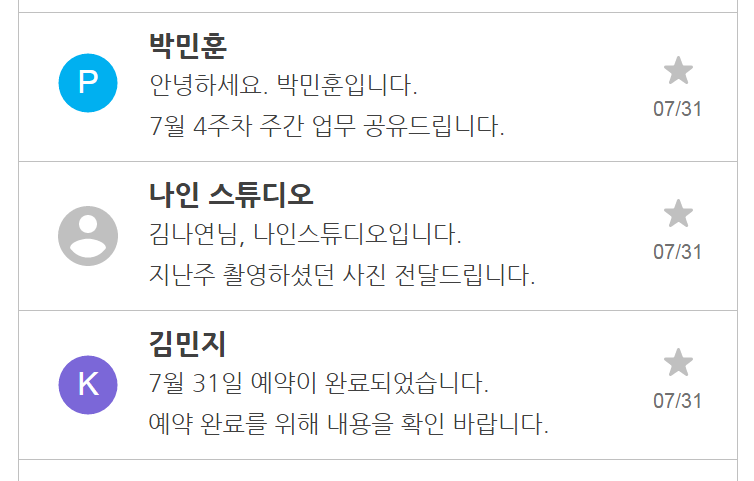
\includegraphics[scale=0.65]{favorite_sample}

사용자는 하나씩 천천히 선택/해제를 하지 않기 때문에, UI를 Blocking하지 않기 위해서 별도 스레드에서 DB에 반영하기로 했다.
그런데 사용자는 선택/해제를 마구 바꾸기도 하는데, 이 때문에 좀 더 세심한 처리가 필요하다.
만일 체크 상태가 바뀔 때마다 스레드를 생성하거나 스레드 풀에서 스레드를 가져다가 DB에 반영하면 어떤 일이 벌어질까? 스레드 실행은 start()를 실행한 순서대로 되지 않기 때문에 선택$\rightarrow$해제$\rightarrow$선택을 했지만, DB에 반영할 때는 선택$\rightarrow$선택$\rightarrow$해제 순으로 반영하여 최종 결과를 잘못 반영할 가능성이 있다. 
즉 실행 순서를 순차적으로 맞추어야 하는데, 바로 HandlerThread가 필요한 지점이다.\footnote{허니콤 이후의 AsyncTask도 순차 실행이 기본 동작이지만, AsyncTask는 백그라운드 스레드와 UI 스레드를 구분하고 데이터를 전달하는 목적에 더 적합하다.}
HandlerThread를 쓰지 않고서 비슷한 동작을 하려면, 백그라운드 스레드에서 무한루프를 만들고 BlockingQueue를 매개로 하여 무한루프문 내에서 take를 실행하고 외부에서 put을 실행하는 형태를 만들어야 한다.
BlockingQueue API 문서에 관련 샘플이 있는데, HandlerThread를 사용하면 구조보다 Message에 더 집중할 수 있다.\\

아래 코드를 한번 보자. 아직 버그가 있는 버전이고 이 버그를 통해 HandlerThread의 구조를 더 잘 이해할 수 있을 것이다.
\newpage
\begin{lstlisting}[frame=single, caption=HandlerThread 사용 예제(버그 존재), label=src:HandlerThreadSample] 
 	private Handler favoriteHandler;
    private Looper favoriteLooper;

    @Override
    public void onCreate(Bundle savedInstanceState) {
       	... 
       	HandlerThread handlerThread 
       		= new HandlerThread("Favorite Processing Thread");
        handlerThread.start(); // (1)
        favoriteLooper = handlerThread.getLooper(); // (2)
        favoriteHandler = new Handler(favoriteLooper) {

            @Override
            public void handleMessage(Message msg) { // (3)
                MessageFavorite messageFavorite = (MessageFavorite) msg.obj;
                favoriteDao.updateMessageFavorite(messageFavorite.id, 
                	messageFavorite.favorite);
            }

        };
        
	}

	private class MessageAdapter extends ArrayAdapter<Message> {
		
		@Override
        public View getView(int position, View convertView, ViewGroup parent) {	
        	...
			holder.favorite.setOnClickListener(new View.OnClickListener() {

                @Override
                public void onClick(View view) {
                    boolean checked = ((CheckBox) view).isChecked();
                    Message message = favoriteHandler.obtainMessage();
                    message.obj = new MessageFavorite(item.id, checked);
                    favoriteHandler.sendMessage(message); // (4)
                }

            });
	}
	
	
	@Override
    protected void onDestroy() {
        if (favoriteLooper != null) {
            favoriteLooper.quit(); // (5)
        }
        super.onDestroy();
    }
\end{lstlisting}

여기서 라인별로 주요한 내용들을 얘기해보자.
\begin{itemize}
\item 9라인(1)에서 HandlerThread를 시작하였다. HandlerThread는 Thread를 상속한 것이라는 걸 기억하자.
\item 10라인(2)에서 Handler를 생성하면서 HandlerThread에서 만든 Looper를 전달하였다.
\item 36라인(4)에서 체크박스를 선택/해제할 때마다 Handler에 Message를 보낸다.
\item 14라인(3)에서 Message를 받아서 DB에 반영한다.
\item 46라인(5)에서 Looper를 종료한다. 
\end{itemize}

작동방식이 그리 어려워 보이진 않는다.
그런데 Looper를 종료할 때 null 체크를 하는 부분은 어째서일까? 
테스트를 여러 번 하다보니 NullPointerException이 발생했는데, 재현도 쉽지 않았던 부분이다. 
Thread에서 start()를 실행하면, 스레드가 바로 시작하는 것이 아니라 스케줄링에 따라 시간차가 있다. 
즉 onCreate() 실행 중에 시작할 수도 있지만, onCreate()가 끝난 이후에도 곧바로 시작한다는 보장도 없다.
이제 메인 스레드 쪽을 보면 onDestory()가 곧바로 불리는 상황이 있다. 
Activity의 onCreate() 안에서 전달된 Intent 파라미터가 유효하지 않을 때 finish()를 호출하는 경우도 있고, onStart(), onResume()에서도 마찬가지다. 
onResume() 메서드까지 어쨌든 실행했는데, 사용자가 ``왜 이리 늦지'' 하면서 Back 키를 누를 수도 있다. Back 키도 디폴트로 finish()를 호출하고, 
finish()를 통해서 onDestroy() 메서드가 호출되는데, onDestory() 실행 이전에 HandlerThread가 시작되는 것을 보장할 수가 없다!
보통 때는 잘 되다가 드물게 NullPointerException이 발생하는 원인이 이것인데, null 체크를 하는 수 밖에 없었다.
그런데 엄밀하게 얘기하면 코드 \ref{src:HandlerThreadSample}도 정확한 코드가 아니다. 
`실행해보니 문제가 생기네' 하면서 시행착오를 넘어간 것 뿐이다.\\

이제 Looper를 제대로 종료하는 방법을 알아보자. 코드 \ref{src:HandlerThreadSample}에는 아직 오류가 있는 것일까?
문제 제기 내용은 2가지이다.\\

\underline{\bfseries 1) Looper.quit()을 쓰는 게 적절한가?}\\
DB 반영 내용이 많아서 시간이 걸린다고 가정해보자. 
사용자가 액션을 빈번하게 보냈을 때 곧바로 처리가 되지 않은 상태에서 Back 키로 종료하면, Looper.quit()에서 아직 처리하지 않은 메시지는 어떻게 하는가?
코드 \ref{src:HandlerThreadSample}에서는 Delayed Message가 없으니까, 굳이 quitSafely()가 아닌 quit()으로 종료해도 문제가 없긴 하다.\\

\underline{\bfseries 2) Looper를 null 체크하는 시점 이후에 스레드가 시작되면 어떻게 되는가?}\\
바로 타이밍 문제가 생긴다. 
Looper.loop() 메소드는 무한루프 상태이고 스레드는 그 스레드를 시작한 Activity를 참조하고 있으므로, onDestroy() 이후에도 Activity는 내내 GC가 안되는 문제가 발생한다.
quit()이나 quitSafely()를 호출해야만 GC 문제가 생기지 않는다.
null 체크를 해도 안되고 안 해도 문제인 상황에 다른 해법이 있을까?\\

MessageQueue.IdleHandler API 문서를 보면, IdleHandler 인터페이스를 가지고서 MessageQueue의 Message를 모두 처리하고서 휴식 상태일 때 할 일을 지정할 수 있다.
인터페이스의 유일한 메서드인 queueIdle()은, IdleHandler를 계속 사용하려면 true를 리턴하고 아니면 false를 리턴한다. 다시 말해서 false를 리턴하면 idle 상태가 될 때마다 queueIdle() 메서드가 실행된다.
결론적으로 IdleHandler를 등록해서 Activity가 종료되고 모든 MessageQueue가 idle 상태가 되었을 때 Looper.quit()을 실행하면 된다.\\

코드 \ref{src:HandlerThreadSample}과 달라지는 부분은 두 군데이다.
\begin{itemize}
\item onDestroy()에서 Looper.quit()을 실행하지 않는다.
\item MessageQueue에 IdleHandler을 등록해서 IdleHandler 안에서 Looper.quit()을 실행한다.
\end{itemize}

달라지는 부분 위주로 코드를 보자.
\begin{lstlisting}[frame=single, caption=Handler 스레드 사용 예제(Fixed), label=src:HandlerThreadSample2] 
 	@Override
    public void onCreate(Bundle savedInstanceState) {
    	...
        HandlerThread handlerThread
                = new HandlerThread("Favorite Processing Thread") {

            @Override
            protected void onLooperPrepared() { // (1)
                getLooper().myQueue().addIdleHandler(
                		new MessageQueue.IdleHandler() {

                    @Override
                    public boolean queueIdle() {
                        if (isFinishing()) { // (2)
                            getLooper().quit();
                            return false;
                        }
                        return true;
                    }

                });
            }

        };
        handlerThread.start();
        ...
	}
	
	@Override
    protected void onDestroy() {
        super.onDestroy();
    }
\end{lstlisting}

\begin{itemize}
\item 8라인(1)에서 IdleHandler를 등록한다. onLooperPrepared() 메서드는 HandlerThread에서 일종의 hook 메서드로 Looper.prepare()가 실행된 다음에 호출된다.
\item 14라인(2)에서 isFinishing() 메서드로 종료 여부를 체크한다. isFinishing() == true인 경우에는 Looper를 종료하고, IdleHandler를 더 쓸 필요가 없으므로 queueIdle() 메서드는 false를 리턴한다.
\end{itemize}

\begin{comment}    
% 이 경우는 Thread 안에서 Handler를 쓰는 것이 낫다.
서버에서 데이터를 가져와서  로컬 데이터베이스에 넣는데 카테고리와 상세를 각각 가져온다고 하자.
카테고리가 먼저 입력되어야만 Foreign Key Contraint 문제가 발생하지 않는데, 각각 스레드로 병렬 실행한다면 상세 데이터를 먼저 가져와서 문제가 발생할 수 있다. 이런 경우에 순차 입력을 위해서 HandlerThread를 고려해보자.\\

라이브러리를 사용하면서 순차적으로 작업들을 실행할 때도 있다. 이때 하나가 끝나면 Listener에서 다음 작업을 실행하도록 만들거나, 만들어진 것을 본 적이 있을 것이다. 이런 경우도 HandlerThread를 사용하고 도중에 실패한 경우에는 HandlerThread의 quit() 메서드를 호출한다.
\end{comment}

\section{스레드 풀}
\subsection{ThreadPoolExecutor}
스레드를 만들려면 Thread를 상속하거나 Thread(Runnable) 생성자에 Runnable 을 넘기는 방법이 있다. 그리고 또 한 가지는 스레드 풀을 사용하는 방법도 있다.
스레드 풀은 대기 상태의 스레드를 유지해서 태스크 실행 오버헤드를 줄임으로써 많은 개수의 비동기 작업을 실행할 때 퍼포먼스를 향상시킨다. 
그리고 스레드를 포함한 리소스를 제한하고 관리하는 방법도 제공한다. 
컴포넌트에 작업이 계속 들어온다면 스레드 풀 사용을 고려해보자. AsyncTask도 내부적으로 스레드 풀을 사용하고 있다.\\

ThreadPoolExecutor에는 4개의 생성자가 있는데 ThreadFactory가 빠져있는 세 번째 생성자 위주로 보자.\\

ThreadPoolExecutor(int corePoolSize, int maximumPoolSize, long keepAliveTime, TimeUnit unit,\\ BlockingQueue<Runnable> workQueue, RejectedExecutionHandler handler)\\

파라미터 가운데서 corePoolSize나 maximumPoolSize는 이름만으로 이해될 것이다. 
pool의 스레드 개수가 coreSize보다 커진다면, 초과하는 개수만큼의 작업은 끝나고 나서는 스레드를 유지할 필요는 없다. 
조금 혼동되는 부분이 ThreadPoolExecutor 생성자에서 corePoolSize만큼 미리 생성하는가 하면 그렇지는 않다. 해당 용도의 메서드는 prestartCoreThread()로 필요하면 별도로 호출할 수 있다. 기본적으로 execute()나 submit()을 호출하는 순간에 실행중인 스레드 개수가 corePoolSize보다 적으면 새로 스레드를 추가하는 형태이다.
keepAliveTime과 unit은 이때 바로 제거하지 않고 대기하는 시간이다. 보통 unit에는 TimeUnit.MINUTES나 TimeUnit.SECONDS를 사용한다.
workQueue도 내용상 중요하다. pool에서는 corePoolSize 개수만큼 유지하려 하고 추가로 요청이 들어오면 workQueue에 쌓는다. 
% 이 workQueue 개수 제한이 넘으면 pool의 스레드 개수를 늘리는 것을 고려해야 한다. 별도 라인에서 따로 설명?
workQueue에 쓸 수 있는 것은 세 가지이다.
\begin{itemize}
\item ArrayBlockingQueue: Queue 개수 제한이 있으며 요청이 들어오면 일단 Queue에 쌓는다. Queue가 꽉 차서 더 넣을 수 없는 경우에는 maximumPoolSize가 될 때까지 스레드를 하나씩 추가해서 사용한다
\item LinkedBlockingQueue: 일반적으로 Queue 개수에 제한이 없다. 들어오는 요청마다 계속해서 쌓는데 이 경우에는 maximumPoolSize가 의미가 없다. LinkedBlockingQueue도 LinkedBlockingQueue(int capacity) 생성자를 사용해서 Queue 개수에 제한을 둘 수는 있다.
\item SynchronousQueue: 요청을 쌓지 않고 바로 준비된 스레드로 처리한다. 결국 Queue를 안 쓴다는 의미이다.
모든 스레드가 작업중이라면 maximumPoolSize까지는 스레드를 생성해서 처리한다. 
\end{itemize}

ThreadPoolExecutor가 shutdown되거나, 최대 스레드 개수와 workQueue 용량을 초과할 때는 때는 태스크가 거부된다. 거부되는 방식을 정하는 것이 ThreadPoolExecutor 생성자의 마지막 파라미터인 RejectedExecutionHandler이고 미리 정의된 4개가 있다.
\begin{itemize}
\item ThreadPoolExecutor.AbortPolicy: 디폴트 handler로 RejectedExecutionException 런타임 예외를 발생시킨다.
\item ThreadPoolExecutor.CallerRunsPolicy: 스레드를 생성하지 않고 요청 태스크를 호출하는 스레드에서 바로 실행된다. 
\item ThreadPoolExecutor.DiscardPolicy: 요청 태스크가 조용히 제거된다.
\item ThreadPoolExecutor.DiscardOldestPolicy: workQueue에서 가장 오래된 태스크를 제거한다.
\end{itemize}

AsyncTask.THREAD\_POOL\_EXECUTOR도 RejectedExecutionHandler를 따로 넣지 않아서 기본으로 AbortPolicy가 적용된다. AsyncTask는 기존에는 maximumPoolSize = 128과 workQueue 개수 = 10으로 지정되어 있었고, 킷캣부터 maximumPoolSize = (CPU 개수 * 2 + 1)과 workQueue 개수 = 128로 변경되었는데, 어쨌든 maximumPoolSize + workQueue 개수를 넘으면 에러가 발생한다. 파일 사이즈가 큰 이미지들을 AsyncTask를 이용해서 한꺼번에 다운로드한다면 발생 케이스를 재현해볼 수 있다.\\

앱에서 ThreadPoolExecutor를 사용할 때는 가장 쓸모 있는 RejectedExecutionHandler는 DiscardOldestPolicy이다. 
화면에서 계속 스크롤하거나 다른 화면으로 이동할 때, 지금 보여지는 화면이 중요하고 이미 지나가버린 것은 상대적으로 중요하지 않다. 
DiscardOldestPolicy를 사용하면 오래된 것을 workQueue에서 제거하고 최신 태스크를 workQueue에 추가한다. 
아래 샘플은 ImageView에 표시할 이미지 파일을 다운로드해서 보여줄 때, DiscardOldestPolicy를 사용한 예이다.
ListView의 각 아이템에 ImageView가 있을 때, 현재 스크롤된 위치에서 ImageView의 url이 workQueue의 마지막에 들어가고 workQueue 사이즈를 초과하는 경우 스크롤된 지 오래된 ImageView의 url은 제거된다.
\begin{lstlisting}[frame=single] 
	private static final int FIXED_THREAD_SIZE = 4;
	private static final int QUEUE_SIZE = 20;
	
	private ThreadPoolExecutor executor
		= new ThreadPoolExecutor(FIXED_THREAD_SIZE, FIXED_THREAD_SIZE, 
				0L, TimeUnit.MILLISECONDS, 
				new LinkedBlockingQueue<Runnable>(QUEUE_SIZE), 
				new ThreadPoolExecutor.DiscardOldestPolicy());
	
	private void queueDownload(ImageView imageView, String url) {
		executor.submit(new ImageDownloadTask(imageView, url));
	}
\end{lstlisting}
스레드 개수는 4개를 쓰고 workQueue 사이즈는 20개이므로, 동시에 24개까지는 태스크를 집어넣을 수 있다. 그 이상으로 submit()을 실행하면 workQueue에서 오래된 태스크를 제거하고서 새로운 태스크를 workQueue에 추가한다.\\
	
\subsection{ScheduledThreadPoolExecutor}
지연/반복 작업에 대해서는 ScheduledThreadPoolExecutor를 사용할 수 있다.
앞에서 Handler를 이용해도 지연/반복 작업을 할 수 있다고 했는데, 화면 갱신이라면 Handler를 쓰는 게 적절하지만 네트워크 통신이나 DB 작업 같은 것이 지연/반복 실행되는 경우는 ScheduledThreadPoolExecutor를 고려하자.\\

다른 옵션으로 Timer를 생각할 수도 있지만 Timer API 문서를 보면 Timer보다는 ScheduledThreadPoolExecutor를 사용하도록 권장한다. Timer는 실시간 태스크 스케줄링을 보장하지 않고(스레드를 하나만 생성해서 사용하기 때문에 앞서 실행되는 작업 때문에 예정 시간에 맞지 않게 실행될 수 있다), 여러 스레드가 동기화 없이 하나의 타이머를 공유하는 문제가 있다.\footnote{자바 병렬 프로그래밍 6.2.5에 관련해서 상세한 내용이 나와있다.}\\

ScheduledThreadPoolExecutor도 ThreadPoolExecutor와 마찬가지로 4개의 생성자가 있는데, ThreadPoolExecutor에 있는 maximumPoolSize, keepAliveTime, unit, workQueue 4개의 파라미터가 빠져 있다. 
이 4개는 ScheduledThreadPoolExecutor에서 고정되어 있는데,
maximumPoolSize = Integer.MAX\_VALUE, keepAliveTime = 0, workQueue에는 내부 클래스인 DelayWorkQueue 인스턴스가 전달된다.
DelayWorkQueue는 기본 사이즈는 16인데, 들어오는 게 많아지면 계속 사이즈가 커지고 제한이 없다.\\

ScheduledThreadPoolExecutor의 사용 예는 \ref{subsec:messenger}절에서 볼 수 있다.

\begin{comment}
public ScheduledFuture<?> schedule(Runnable command, long delay, TimeUnit unit)
public ScheduledFuture<V> schedule(Callable<V> callable, long delay, TimeUnit unit)
public ScheduledFuture<?> scheduleAtFixedRate(Runnable command, long initialDelay, long period, TimeUnit unit)
public ScheduledFuture<?> scheduleWithFixedDelay(Runnable command, long initialDelay, long delay, TimeUnit unit)
\end{comment}

\subsection{Executors}
ThreadPoolExecutor, ScheduledThreadPoolExecutor는 직접 생성하는 것보다는 Executors의 팩토리 메서드로 생성하는 경우가 많다.
Executors에서 리턴하는 ExecutorService, ScheduledExecutorService는 ThreadPoolExecutor, ScheduledThreadPoolExecutor의 상위 인터페이스이다.\\

Executors의 주요 팩토리 메서드는 아래와 같다.
\begin{itemize}

\item newFixedThreadPool(int nThreads): 파라미터로 전달되는 고정 개수까지 스레드를 생성한다. workQueue는 크기 제한이 없다.
\begin{lstlisting}[frame=single] 
new ThreadPoolExecutor(nThreads, nThreads, 0L, TimeUnit.MILLISECONDS, 
    new LinkedBlockingQueue<Runnable>())
\end{lstlisting}

\item newCachedThreadPool(): 필요할 때 스레드를 생성하고 스레드는 개수 제한이 없다. keepAliveTime이 60초로 길다는 것이 특징이다. 이 때문에 Cached라는 수식어가 붙었다.
\begin{lstlisting}[frame=single] 
new ThreadPoolExecutor(0, Integer.MAX_VALUE, 60L, TimeUnit.SECONDS, 
    new SynchronousQueue<Runnable>());
\end{lstlisting}

\item newSingleThreadExecutor(): 단일 스레드를 사용해서 순차적으로 처리한다. workQueue는 크기 제한이 없다. 
\begin{lstlisting}[frame=single] 
new FinalizableDelegatedExecutorService(
	new ThreadPoolExecutor(1, 1, 0L, TimeUnit.MILLISECONDS, 
	new LinkedBlockingQueue<Runnable>())
\end{lstlisting}
newFixedThreadPool(1)과 동일한 결과를 리턴하는 것으로 보이는데, 다시 FinalizableDelegatedExecutorService로 Wrapping하였다. Wrapping의 효과는 스레드 개수를 1이 아닌 다른 값으로 변경하지 못하게 하는 것이다. 단순히 newFixedThreadPool(1)로 리턴된 것은 ThreadPoolExecutor로 캐스팅해서 setCorePoolSize()나 setMaximumPoolSize() 메서드로 스레드 개수를 변경할 수 있다.

\item newScheduledThreadPool(int corePoolSize): corePoolSize 개수의 ScheduledThreadPoolExecutor를 만든다.
\begin{lstlisting}[frame=single] 
new ScheduledThreadPoolExecutor(corePoolSize)
\end{lstlisting}

\end{itemize}

팩토리 메서드 가운데서 용도에 맞는 게 없다면 결국 ThreadPoolExecutor, ScheduledThreadPoolExecutor를 직접 사용해야만 한다.\\

\section{AsyncTask}
\label{sec:asynctask}
동시성 프로그래밍에 익숙하지 않은 경우에는 안드로이드 API에 과도하게 의존하는 경우도 있다.
예를 들어, Service에서 시간이 오래 걸리는 작업이라면 단순하게 스레드를 생성해서 실행하면 되는데, AsyncTask를 생성해서 doInBackground() 메서드만을 구현하는 케이스도 볼 수 있다. 
AsyncTask는 백그라운드 스레드에서 작업하는 진행 상태나 결과 데이터를 UI 스레드에 전달하고, 백그라운드 스레드와 UI 스레드를 고민하지 않고 구분해서 쓸 수 있도록 만들어진 것이다.
AsyncTask는 onPostExecute() 오버라이드가 필요하지 않을 때는, 즉 UI 작업이 필요하지 않는 경우 쓰지 않는 게 좋다. 이때는 AsyncTask의 스레드 풀을 사용하는 것뿐이다.

백그라운드 스레드와 UI 스레드를 구분해서 사용하는 여러 방법을 살펴보자.
\begin{lstlisting}[frame=single] 
	public void onClick(View v) {
    	new Thread(new Runnable() {
    		
    		@Override
        	public void run() {
            	Bitmap b = loadImageFromNetwork("http://example.com/image.png");
            	mImageView.setImageBitmap(b);
        	}
        	
    	}).start();
	}
\end{lstlisting}
백그라운드 스레드에서 UI를 변경하므로 CalledFromWrongThreadException이 발생한다.
이를 해결하는 방법은 앞에서도 얘기했듯이 여러 버전이 있다.

\begin{enumerate}
\item Handler 이용(2가지 방식)
\begin{lstlisting}[frame=single]
	private final static int BITMAP_MSG = 1;
	
	private Handler mHandler = new Handler() {
		
		@Override
		public void handleMessage(Message msg) {
			if (msg.what == BITMAP_MSG) {
				mImageView.setImageBitmap((Bitmap) msg.obj);
			}
		}
		
	};
	
	public void onClick(View v) {
    	new Thread(new Runnable() {
    		
    		@Override
        	public void run() {
            	final Bitmap bitmap 
            		= loadImageFromNetwork("http://example.com/image.png");
            	Message message = Message.obtain(mHandler, BITMAP_MSG, bitmap);
            	mHandler.sendMessage(message);
        	}

	
    	}).start();
	}
\end{lstlisting}

\begin{lstlisting}[frame=single]
	private Handler mHandler = new Handler();
	
	public void onClick(View v) {
    	new Thread(new Runnable() {
    	
    		@Override
        	public void run() {
            	final Bitmap bitmap 
            		= loadImageFromNetwork("http://example.com/image.png");
            	mHandler.post(new Runnable() {
            		
                	public void run() {
                    	mImageView.setImageBitmap(bitmap);
                	}
                	
            	});
        	}

	
    	}).start();
	}
\end{lstlisting}

\item View의 post() 메서드에 Runnable 전달: 내부적으로 Handler를 사용한다. Activity의 runOnUiThread() 메서드도 동일한 형태로 사용하면 된다.
\begin{lstlisting}[frame=single] 
	public void onClick(View v) {
    	new Thread(new Runnable() {
    	
    		@Override
        	public void run() {
            	final Bitmap bitmap
            		= loadImageFromNetwork("http://example.com/image.png");
            	mImageView.post(new Runnable() {
                	public void run() {
                    	mImageView.setImageBitmap(bitmap);
                	}
            	});
        	}
        	
    	}).start();
	}
\end{lstlisting}
	
\item AsyncTask 이용: 내부적으로 Handler를 이용한 첫 번째 방식으로 되어있다.
\begin{lstlisting}[frame=single]
	public void onClick(View v) {
    	new DownloadImageTask().execute("http://example.com/image.png");
	}

	private class DownloadImageTask extends AsyncTask<String, Void, Bitmap> {
	
		@Override
    	protected Bitmap doInBackground(String... urls) {
        	return loadImageFromNetwork(urls[0]);
    	}

      	@Override
    	protected void onPostExecute(Bitmap result) {
        	mImageView.setImageBitmap(result);
    	}
    	
	}	
\end{lstlisting}
\end{enumerate}
여기 샘플에서 빠진 부분이 있다. 바로 loadImageFromNetwork() 메서드에 대한 예외 처리가 없는데 이 내용은 뒤에서 이슈로 살펴보겠다.\\

AsyncTask는 제네릭 클래스이고 타입 파라미터에는 Params, Progress, Result 세 가지가 있다. 진행 상태가 필요하지 않은 경우 Progress에 Void가 들어가는 경우는 있지만 모두 다 Void인 것도 권장되는 형태는 아니다.\\

아래는 개발자 가이드에 있는 내용이다.
\begin{lstlisting}[frame=single]
private class MyTask extends AsyncTask<Void, Void, Void> { ... }
\end{lstlisting}
이것은 백그라운드 스레드와 UI 스레드를 구분하기 위한 용도로만 쓰이는 것으로 Handler를 이용하는 게 더 단순할 수 있다.\\

AsyncTask는 안드로이드 개발자에게는 익숙한 것이기 때문에 이 절에서는 이슈 중심으로 살펴보자.

\subsection{병렬 실행 시 실행 순서}
안드로이드 버전이 올라가면서 많은 논란이 있던 내용 가운데 하나가 AsyncTask를 실행할 때 기본 동작이 `병렬 실행'에서 `순차 실행'으로 바뀐 것이다. 
병렬 실행이 여러 문제를 일으켰기 때문에, 제어 가능하다고 자신하는 경우에만 `병렬 실행'을 쓰라는 의미이다.
그럼에도 여전히 AsyncTask는 병렬 실행을 기본으로 해서 개발할 때가 많다.\\

AsyncTask의 병렬 실행이 필요한 경우를 들어보자. 
화면에 여러 가지 정보를 보여주는 데 DB나 서버 API로 단번에 가져오지 못하는 경우가 많다. 도착 지점의 날씨 정보와 주변 주차장 정보를 화면에 보여주고 싶은데 서버 API가 따로라면 API를 병렬로 호출하는 게 유리할 것이다.\\

2개 이상을 동시에 실행하는 경우도 있겠지만 일단 2개로 제한해서 얘기를 진행하자.   
2개의 AsyncTask를 시작하면 메인 스레드에서 동작하는 onPostExecute()는 단일 스레드 규칙에 의해 하나씩 실행이 되지만 2개의 AsyncTask 가운데 어느 것이 먼저 doInBackground()를 먼저 끝내고 onPostExecute()를 실행할 지는 알 수 없다. 
예를 들어, 필자는 동일한 데이터 구조를 로컬에서 가져온 것과 API를 통해 서버에서 가져온 것을 조합해서 화면에 보여준 적이 있다. 
2개를 각각 AsyncTask로 만들고 로컬 데이터를 가져오는 것을 먼저 시작하고(AsyncTaskA) 서버 데이터를 가져오는 것을 바로 다음에 시작하였다(AsyncTaskB). 
로컬 데이터가 결과를 빨리 가져온다는 가정하에 AsyncTaskA에서는 멤버 변수에 데이터만 저장하고 AsyncTaskB의 onPostExecute()에서 조합해서 화면을 보여주었다.
결과는 어땠을까? 아주 드물지만 로컬 데이터를 먼저 가져온다는 가정이 어긋나는 경우가 생겨서 에러를 발생시켰다. 
작업량이 많고 적은 것으로 판단하면 안된다.
백그라운드 스레드 간에는 무엇이 먼저 실행된다고 가정하면 안된다. 극단적으로 말하면 정상 동작 여부가 운에 따른 것이 된다.
이런 문제가 제어가 어렵다면 차라리 `순차 실행'을 하는 게 나을 수도 있다.\\

일반적으로 2개의 AsyncTask 간에 병렬 실행도 하면서 결과를 합해야 하는 경우에는 2가지 정도 방법을 사용한다.
\begin{itemize}
\item 멤버 변수에 비트 OR 연산을 사용한다. 2개의 AsyncTask가 끝나면 각각 비트를 합하고 둘 다 충족했다면 onPostExcecute() 메서드에서 데이터를 조합해서 보여준다. 예외가 나오는 케이스도 고려해야만 한다. 
\item CountDownLatch를 이용해서 AsyncTask 간에 다른 한 쪽의 작업이 끝날 때까지 대기했다가 이후에 데이터를 조합한다. 이 방식은 \url{http://suribada.com/wp/?p=13}을 참고하자.
\end{itemize}

AsyncTask의 대안으로 RxJava 라이브러리를 사용하기도 한다. RxJava에 대한 내용은 \url{https://github.com/ReactiveX/RxJava/wiki}를 참고하자.

\subsection{Activity 종료 시점과 불일치}
Activity에서 AsyncTask의 백그라운드 작업 실행 도중에 Back 키를 통해서 Activity를 종료하면 AsyncTask는 어떻게 되는가? 메모리에는 Activity가 남아있어서 onPostExecute()도 정상적으로 실행되고 그 안에서 setText()와 같은 UI 변경 메서드도 잘 실행된다. 다만 눈앞에서 사라져서 보이지 않을 뿐이다.
이렇게 Activity 종료 시점과 AsyncTask가 끝나는 시점이 달라서 발생하는 문제가 몇 가지 있다.\\

\begin{itemize}
\item 메모리 문제가 발생할 수 있다. Activity가 Back 키로 종료할 때는 AsyncTask가 오래 걸리는 게 아니라면 큰 문제까지는 아니다. 
AsyncTask 때문에 문제가 생기는 것은 화면 회전으로 인해 계속해서 AsyncTask가 쌓여서 실행하는 경우이다.
Activity가 화면 방향 고정이거나 android:configChanges 속성에 ``orientation''이 들어있지 않은 경우 화면 회전 시마다 Activity는 종료되고 새로 시작되는데 새로 시작되는 것은 다른 인스턴스이다. 
AsyncTask가 아직 실행 중인 경우에는 기존 Activity도 메모리에서 제거되지 않는다. 빈번하게 화면을 회전할 때 OutOfMemoryError가 발생하는 원인 가운데 하나가 될 수 있다.
`안드로이드 멀티스레딩' 책에서 제안한 방법은 Activity를 WeakReference로 한 정적 내부 클래스로 AsyncTask를 만드는 것인데, 번거로워서 쓰기에 망설여진다. Activity가 종료될 때 AsyncTask를 함께 종료하는 방법을 찾아보는 게 좋겠다. 이에 대해서는 바로 다음 절에서 살펴보자.  
또 다른 대안으로는 Loader 프레임워크를 사용하는 방법도 있다.\footnote{\url{http://developer.android.com/intl/ko/guide/components/loaders.html} 내용을 참고하자.}
Loader 사용은 복잡하지만 충분히 고려할 만하다. 

\item AsyncTask를 순차 실행한다면(SERIAL\_EXECUTOR) 화면 회전 시마다 작업이 쌓이므로 갈수록 실행이 느려질 수 있다.

\item Fragment에서 AsyncTask를 실행할 때 문제가 발생할 수 있다. AsyncTask 실행 도중에 Back 키로 Activity를 종료하면 Fragment는 Activity와 분리되면서 Fragment에서 getActivity()는 null을 리턴한다. AsyncTask의 onPostExecute()에서 Context를 사용할 때 NullPointerException이 발생하므로, 권장되는 방식은 onPostExecute() 메서드 시작 부분에서 getActivity() == null을 체크해서 리턴하는 것이다. 어차피 화면이 없으므로 UI를 업데이트하지 않고 리턴하는 것이 적절하다. 
\end{itemize}

\subsection{AsyncTask 취소}
AsyncTask에는 cancel() 메서드가 있다. 이 메소드는 AsyncTask의 mCancelled 변수를 true로 만들고, 이로 인해 스레드 작업 이후에 onPostExecute() 대신 onCancelled()가 불린다. 스레드 작업이 오래 걸리는 경우에 doInBackground() 메서드에서는 중간에 isCancelled() 메서드로 체크해서 바로 리턴하는 로직을 쓰는 것을 권장하고 있다. 무엇을 리턴하든 간에 onPostExeceute()는 불리지 않고 onCancelled()에서 처리한다.\footnote{허니콤부터 onCancelled() 메서드는 파라미터가 없는 버전에 doInBackground()의 결과를 전달하는 onCancelled(Result result) 메서드가 추가되었다.}\\

결론적으로 AsyncTask를 Activity 종료 시점에 근접하게 종료하는 방법은 isCancelled() 메서드를 doInBackground()에서 곳곳에 사용하고(특히 루프문에서), AsyncTask를 멤버 변수로 유지하고서 Activity의 onDestroy()에서 AsyncTask의 cancel() 메서드를 호출하는 것이다.\\

%mayInterruptIfRunning 파라미터에 true를 전달하면 무엇이 다를까? 이것은 스레드에 인터럽트 신호를 보내는 것으로 스레드가 바로 종료하는 것은 아니다.
% 사용하는 클래스에서 사용?(예로 소켓 종료)
% sleep 샘플(sleep 문제...)

\subsection{예외 처리 메서드 부재} 
AsyncTask에는 정상적인 데이터 처리를 위한 onPostExcecute()와 작업 취소를 위한 onCancelled() 메서드는 있는데 예외 처리를 위한 onError() 메서드는 없다. 
백그라운드 스레드에서 하는 작업은 네트워크 문제와 같은 다양한 예외 케이스가 있어서, 이 경우에는 문제가 발생했다고 화면에 표시하는 경우가 많다. 즉 예외 케이스에도 UI 작업이 필요한 것이다.\\

백그라운드 스레드와 UI 스레드를 분리할 때 예외에 대해서도 고려가 필요한데, 이 내용이 AsyncTask에서 빠져서 AsyncTask의 기본 형태를 변형해서 사용하는 경우가 생겼다.
\begin{lstlisting}[frame=single]
	public void onClick(View v) {
    	new DownloadImageTask().execute("http://example.com/image.png");
	}

	private class DownloadImageTask extends AsyncTask<String, Void, Bitmap> {
	
		@Override
    	protected Bitmap doInBackground(String... urls) {
    		try {
        		return loadImageFromNetwork(urls[0]);
        	} catch (Exception e) {
        		return null; // (1)
        	}
    	}

      	@Override
    	protected void onPostExecute(Bitmap result) {
    		if (result == null) { // (2)
    			// show error message at UI
    			return;
    		}
        	mImageView.setImageBitmap(result);
    	}
    	
	}	
\end{lstlisting}
예외가 발생할 때 12라인(1)에서 null을 리턴하고 18라인(2)에서 체크해서 null이면 에러 메시지를 보여주는 식이다. 이 방식도 문제가 완전히 해결된 것은 아니다. 
loadImageFromNetwork()에서 예외는 발생하지 않지만 null을 리턴하는 경우가 있다면, error message가 의도에 맞지 않는다. 예외 상황이 아니면 null이 나올 수 없도록 하거나, 어쨌든 null이 나오는 것을 문제로 간주한다면 가능한 방식이다. 

\begin{lstlisting}[frame=single]
	public void onClick(View v) {
    	new DownloadImageTask().execute("http://example.com/image.png");
	}

	private class DownloadImageTask extends AsyncTask<String, Void, Boolean> {
	
		private Bitmap bitmap;
		
		@Override
    	protected Bitmap doInBackground(String... urls) {
        	try {
        		bitmap = loadImageFromNetwork(urls[0]);
        		return Boolean.TRUE;
        	} catch (Exception e) {
        		return Boolean.FALSE;
        	}
    	}

      	@Override
    	protected void onPostExecute(Boolean result) {
    		if (!result) {
    			// show error message
    			return;
    		}
        	mImageView.setImageBitmap(bitmap);
    	}
    	
	}	
\end{lstlisting}
원래 의도와는 다르게 결과값을 doInBackground()에서 onPostExecute()로 전달하는 것이 아니고, 성공 여부를 Boolean 값을 리턴해서 전달하고 있다. 
전달하고자 하는 결과값은 뜬금없이 AsyncTask의 멤버 변수에 대입돼서 onPostExecute()에서 사용한다.
가능한 방식이긴 하지만 원래 AsyncTask의 사용 방식과 차이가 생긴다.\\
%3가지 패턴(Handler, tuple, 멤버 변수, true, false)

군더더기 코드가 생겨나는데 이에 대한 대안으로 앞에서도 언급한 RxJava를 사용하기도 한다. RxJava에서는 예외에 대한 처리 방법을 기본으로 제공한다.
%http://www.javalobby.org/java/forums/t83677.html Interruptible Method
%http://stackoverflow.com/questions/4767553/safe-use-of-httpurlconnection
% http://www.androiddesignpatterns.com/2012/07/loaders-and-loadermanager-background.html


\chapter{Context}
앱을 개발하다보면 항상 Context 클래스를 만나게 된다. Context가 없으면 Activity를 시작할 수도, Broadcast를 발생시킬 수도, Service를 실행할 수도 없다. 리소스에 접근할 때도 Context를 통해야만 가능하다.
Context를 통해서 여러 컴포넌트가 연결돼있고 Context는 여러 컴포넌트의 상위 클래스이기도 하므로, Context 자체에 대해서 살펴보는 것은 컴포넌트를 이해하는 데도 도움이 된다.\\

Context는 추상 클래스인데 메서드 구현이 거의 없고 상수 정의와 추상 메서드로 이루어진다. 
그럼 Context의 하위 클래스는 어떤 게 있는가? 주요한 것을 얘기하면, 직접 상속한 것은 ContextWrapper이고 ContextWrapper를 상속한 Activity, Service, Application이 있다(BroadcastReceiver, ContentProvider는 Context를 상속한 것이 아니다).\\

% http://blog.naver.com/PostView.nhn?blogId=huewu&logNo=110085457720&parentCategoryNo=&categoryNo=&viewDate=&isShowPopularPosts=false&from=postView

ContextWrapper 클래스에는 그 이름처럼 ContextWrapper(Context base) 생성자를 갖고 있다.
\begin{lstlisting}[frame=single, caption=ContextWrapper.java]
    Context mBase;

    public ContextWrapper(Context base) { // (1)
        mBase = base;
    }

	protected void attachBaseContext(Context base) { // (2)
        if (mBase != null) {
            throw new IllegalStateException("Base context already set");
        }
        mBase = base;
    }
    
    public Context getBaseContext() {
        return mBase;
    }
    
    ...
    
    @Override
    public Context getApplicationContext() {
        return mBase.getApplicationContext(); // (3)
    }
    
    ...
    
    @Override
    public void startActivity(Intent intent, Bundle options) {
        mBase.startActivity(intent, options); // (4)
    }
    
    ...
    
    @Override
    public void sendBroadcast(Intent intent) {
        mBase.sendBroadcast(intent); // (5)
    }

	... 
	
    @Override
    public Resources getResources() {
        return mBase.getResources(); // (6)
    }
\end{lstlisting}
\begin{itemize}
\item 3라인(1), 7라인(2)에서 base 파라미터에 전달되는 것은 Context의 여러 메서드를 직접 구현한 ContextImpl 인스턴스이다. ContextImpl은 앱에서 생성해서 사용할 수 있는 public 클래스는 아니지만, 소스는 공개되어 있으니 한번씩은 살펴보도록 하자
\item ContextWrapper의 여러 메서드는 base의 메서드를 그대로 다시 호출하고 있다(3, 4, 5, 6).
\item Activity, Service, Application은 3라인(1)의 생성자를 사용하지 않고, 실제로는 7라인(2)의 attachBaseContext()를 사용하고 있다.
\end{itemize}

이제 또 다른 질문을 해보자. 그럼 ContextImpl은 앱에서 싱글톤으로 단 하나의 인스턴스를 가지고서 ContextWrapper에 전달하는가?
이것은 ContextWrapper에 getBaseContext()와 getApplicationContext()라는 2개의 메서드가 따로 있는 것을 보면 싱글톤이 아닌 것을 유추해볼 수 있다.\footnote{Context에는 getBaseContext() 메서드는 없고 getApplicationContext() 메서드만 있다.}\\

Activity, Service, Application 각 컴포넌트는 각각 생성한 ContextImpl을 하나씩 Wrapping하고 있고 getBaseContext()는 각각 ContextImpl 인스턴스를 리턴한다. getApplicationContext()는 Application 인스턴스를 리턴하는 것으로 Application은 앱에서 1개 밖에 없고 어디서나 동일한 인스턴스를 반환한다.\\

ContextImpl을 보면 3가지 정도로 메서드 범주를 나눌 수 있다.
\begin{itemize}
\item 앱 패키지 정보, 내/외부 파일, SharedPreferences, 데이터베이스 등과 관련한 Helper 메서드가 있다. 
\item Activity, BroadcastReceiver, Service와 같은 컴포넌트 관련 메서드와 퍼미션 체크 메서드가 있고, 이들 메서드는 system\_server 프로세스의 ActivityManagerService의 메서드를 다시 호출한다. 
\item ActivityManagerService 를 포함한 시스템 서비스에 접근하기 위해서 getSystemService() 메서드가 있다. ContextImpl의 정적 초기화 블록(static initializer block)\footnote{http://warmz.tistory.com/50에서 초기화 블록 내용을 알아보자}에서 클래스가 최초 로딩될 때 시스템 서비스 매핑을 하고, 이후에는 getSystemService() 메서드에서 매핑을 바로 사용하고 있다.
시스템 서비스는 Context 클래스에서 XXX\_SERVICE와 같이 상수명으로 모두 매핑되어 있고, Context가 전달되는 어디서든 getSystemService(Context.ALARM\_SERVICE)와 같이 시스템 서비스를 가져다 쓸 수 있다.
\end{itemize}

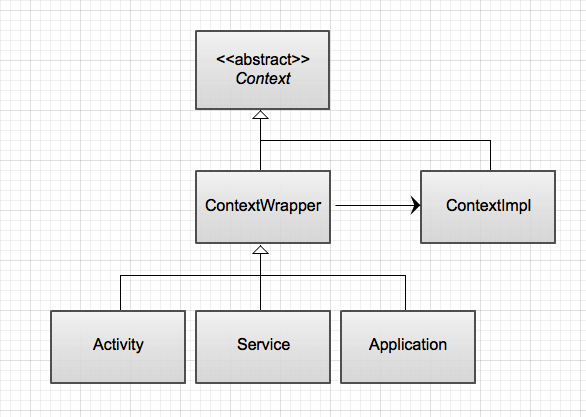
\includegraphics[scale=0.5]{context}\\
객체지향의 원칙에서 상속보다는 구성을 사용하라고 하는데, 이 클래스 다이어그램을 보면 원칙에 들어맞는다.
바로 Activity, Service, Application에서 ContextImpl을 직접 상속하지 않고, ContextImpl의 메서드를 호출하는 형태이다. 이렇게 하면 ContextImpl의 변수가 노출되지 않고, ContextWrapper에서는 ContextImpl의 public 메서드만 호출하게 된다. 또한 각 컴포넌트별로 사용하는 기능에 대한 제어도 단순해진다.\\
%ContextWrapper 소스에 있는 내용

코드에서 Context를 쓰는 방법을 생각해보자.
Activity를 예로 들어보면 여기서 쓸 수 있는 Context 인스턴스는 3개가 된다. 
\begin{enumerate}
\item Activity 인스턴스 자신(this)
\item getBaseContext()를 통해 가져오는 ContexImpl 인스턴스
\item getApplicationContext()를 통해 가져오는 Application 인스턴스: Activity의 getApplication() 메서드로 가져오는 것과 같은 인스턴스이다.
\end{enumerate}

각각의 인스턴스가 다르므로 캐스팅을 함부로 하면 안된다. 이를테면 getBaseContext()로 가져온 것을 Activity로 캐스팅하면 ClassCastException이 발생한다.\\

View 클래스를 보면 생성자에 Context가 들어간다. 이 Context가 어디서 온 것인지 아래 코드를 통해 확인해보자.
\begin{lstlisting}[frame=single]
    @Override
    public void onCreate(Bundle savedInstanceState) {
        super.onCreate(savedInstanceState);
        setContentView(R.layout.main);
        statusView = (TextView) findViewById(R.id.status_view);
        Log.d("suribada", (statusView.getContext() == this));
        Log.d("suribada", (statusView.getContext() == getBaseContext()));
        Log.d("suribada", (statusView.getContext() == getApplicationContext()));
    }
\end{lstlisting}
첫 번째 로그에서만 true가 나오는 것을 볼 수 있다. View 클래스는 생성자에 Context가 전달되어야 한다. 테스트해보면 Activity에서 쓸 수 있는 3가지 Context 모두 다 전달 가능하다. 그러나 View와 연관이 깊은 것은 Activity이므로 Activity를 전달하는 것을 이해할 수 있을 것이다.
내부적으로 setContentView() 메서드에서 사용하는 LayoutInflator에 Activity 인스턴스가 전달되고, View 생성자의 Context 파라미터에 Activity 인스턴스가 전달된다. 


\chapter{Activity}
Activity는 앱에서 화면의 기본단위이고 setContentView() 메서드로 메인 뷰를 화면에 표시한다.
때에 따라 setContentView()를 실행하지 않고, 로직 분기를 해서 다른 Activity를 띄우는 용도로 사용하기도 한다.
한 예로 Intent의 스킴(scheme)에 따라 여러 화면을 호출하는 경우가 있다. 
이때 AndroidManifest.xml에서 여러 Activity에 intent-filter 엘리먼트를 추가하지 않고, Controller 역할의 Activity 1개에만 여러 스킴의 intent-filter를 명시해서 Controller Activity를 거쳐 다른 화면으로 이동시킨다.\\

Activity는 AndroidManifest.xml에 선언해야 호출 가능하다. 
Activity를 설정 파일에 추가할 뿐이지만, 개수가 많으면 유지에 어려움이 있으므로\footnote{규모가 있는 앱은 기능이 변경되면서 쓰지 않는 Activity가 자꾸 생겨나기도 한다. 다행히 근래의 IDE에서는 쓰지 않는 Activity를 표시해주기도 한다.}, Activity는 불필요하게 많이 만들지 않는 것을 권장한다.
내부에 UI 액션이 많고 로직이 많다면 우선 Activity를 고려하고, 
다른 Activity 위에 팝업 형식으로 뜬다면 커스텀 레이아웃 다이얼로그나 DialogFragment, PopupWindow로 대체를 고려하자.
`로딩중'이라고 전체를 덮는 반투명 화면은 어떨까? 이것도 Activity보다는 DialogFragment가 적절하다.
기준은 단순하게 하자. 독립적인 화면이라고 하면 Activity가 더 적합하고, 종속적인 화면으로 보이면 다른 것을 쓸 수 있는지 생각해보자.\\

\section{생명주기}
%http://developer.android.com/training/basics/activity-lifecycle/pausing.html
Activity의 생명주기를 정확히 이해하는 것은 중요하다. 
생명주기를 이해하지 못했을 때 리소스가 반납되지 않을 수도 있고, 필요한 데이터를 읽어들이지 못할 수도 있다.

% http://developer.android.com/guide/topics/fundamentals/activities.html 기본 참고
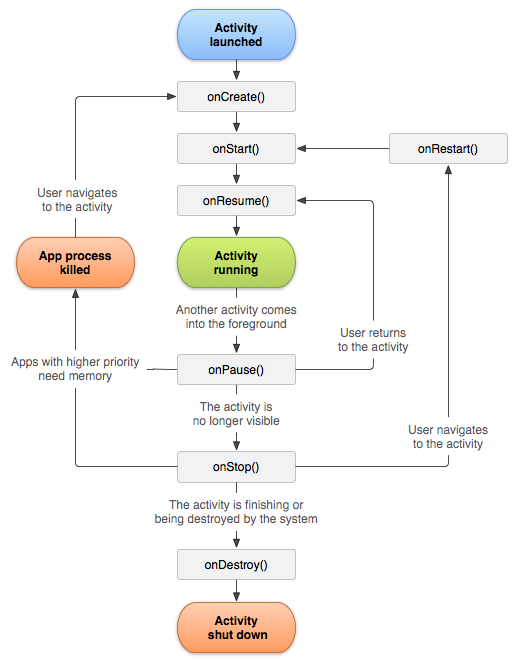
\includegraphics[scale=0.5]{activity-lifecycle}

onStop(), onDestroy() 메서드는 반드시 실행된다는 보장이 없다. 일반적으로 onCreate(), onResume(), onPause() 메서드를 오버라이드하고, 리소스를 안전하게 정리하는 데 필요하다면 onStop()이나 onDestroy()에 안전장치로 코드를 추가하는 경우가 있다.\\

케이스별로 생명주기 메서드가 호출되는 순서를 알아보자.\label{flow}

\fbox{\bfseries 시작할 때}
onCreate $\rightarrow$ onStart $\rightarrow$ onResume\\

\fbox{\bfseries 화면 회전할 때(가로/세로)}
onPause $\rightarrow$ onStop $\rightarrow$ onDestroy $\rightarrow$ onCreate $\rightarrow$ onStart $\rightarrow$ onResume\\

\fbox{\bfseries 다른 Activity가 위에 뜰 때/Power 키로 화면 OFF할 때/Home 키}
onPause $\rightarrow$ onStop\\

\fbox{\bfseries Back 키로 Activity 종료}
onPause $\rightarrow$ onStop $\rightarrow$ onDestroy\\

\fbox{\bfseries Back 키로 기존 Activity에 돌아올 때/Home 키로 나갔다가 돌아올 때}
onRestart $\rightarrow$ onStart $\rightarrow$ onResume\\

\fbox{\bfseries 다이얼로그 테마 Activity가 위에 뜰 때/투명 Activity가 위에 뜰 때}
onPause
\\

메서드가 어디까지 호출되는 지는 visible 상태와 포그라운드 상태를 체크해보면 좀 더 알기 쉽다.
onPause()까지 실행하면 백그라운드이면서 visible 상태이고 onStop()까지 실행되면 not visible 상태이다. 
Activity API 문서에 보면 세 가지 lifetime으로 구분한 내용이 있다.
\begin{itemize}
\item entire lifetime: onCreate() $\sim$
 onDestroy()
\item visible lifetime: onStart() $\sim$
 onStop()
\item foreground lifetime: onResume() $\sim$
 onPause()
\end{itemize}
여기서 혼동되는 게 있다. onCreate() 메서드 내에서 setContentView()에 넣은 레이아웃이 onStart()에서부터 화면에 보이는 것일까? 그렇지 않다. 
onCreate()부터 onResume()까지는 하나의 Message 처리이므로, onResume() 이후에나 ContentView가 화면에 보인다.
onStart()부터 visible lifetime이라는 것은 화면에 보이지 않다가 다시 보일 때는 여기부터 실행된다는 의미이다.
onResume()도 마찬가지이다. background visible 상태(투명 Activity나 다이얼로그 테마 Activity가 가린 경우)에 있다가 foreground로 오면 onResume()부터 실행된다.\\

위 그림은 생명주기 메서드 위주로 표현했고, 아래 그림은 상태 위주로 표현한 것이다.\\
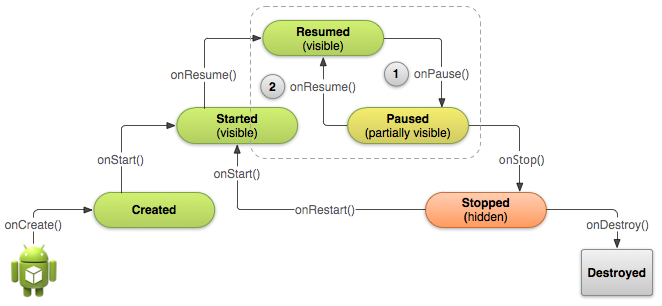
\includegraphics[scale=0.5]{basic-lifecycle-paused}

또 다른 케이스를 들어보자.
\begin{enumerate}
\item onCreate()에서 finish()를 호출하면 다른 생명주기 메서드를 거치지 않고 곧바로 onDestroy()를 실행한다.
\item onActivityResult()는 onResume()보다 먼저 실행된다.
이 순서가 필요할 때가 있다. onActivityResult()에서 가져온 결과를 업데이트하고
onResume()에서도 최신 데이터를 업데이트하려고 할 때, 순서를 유념해야 한다.
\end{enumerate}

Activity에는 onPostCreate()나 onPostResume() 같은 메서드도 있어서 앞에서 얘기한 생명주기 메서드 사이에 뭔가를 할 수도 있지만, 시스템에서 초기화를 위해서 사용하는 것으로 일반적으로 앱에서는 쓰지 않도록 가이드하고 있다.

\subsection{startActivity()와 startActivityForResult()}
Activity를 시작하는 방법은 startActivity()와 startActivityForResult() 메소드를 호출하는 것이다. 대부분 Activity에서 다른 Activity를 시작하고 특별한 경우에 다른 컴포넌트에서 Activity를 시작한다.\\

어떤 책에서는 호출하는 쪽을 부모 Activity라고 하고, 호출되는 쪽을 자식 Activity라고 하는데 혼동스런 표현이다. TabActivity와 같은 ActivityGroup이 부모 Activity이고, 탭 위치에 들어가는 하위 Activity가 자식 Activity이다. Activity에도 getParent() 메서드가 있는데 이것은 자신을 포함(embed)한 Activity를 가리키는 것이지 자기를 호출한 Activity를 가리키는 것이 아니다. 
Activity에 getCallingActivity()와 getCallingPackage() 메서드가 있어서 이 관계를 더 잘 나타내는 말인 듯하여, 이 책에서는 Caller(호출자)와 Callee(피호출자)로 정하고 부르도록 한다.\\

startActivity()는 Callee에 데이터를 전달하기만 하고 Caller에게 다시 데이터를 전달하는 어떤 액션도 하지 않는다.
startActivity() 메서드는 Context의 메서드이므로 Activity뿐만 아니라 Service, BroadCastReceiver, Application 어디서든 startActivity()를 실행할 수 있다.
startActivity()로 시작된 Callee에서는 getCallingActivity()와 getCallingPackage() 메서드는 null을 리턴한다.

startActivityForResult()는 Activity의 메서드다. Activity끼리만 데이터를 주고받을 수 있다고 이해하자. 
startActivityForResult() 메서드 관련해서 몇 가지 내용을 살펴보자.
\begin{itemize} 
\item Callee에서 getCallingActivity()와 getCallingPackage() 메서드는 Caller의 정보를 리턴한다. Caller에 따라 다른 처리가 필요한 경우 구분을 위해 이용할 수 있다. 
\item startActivityForResult(Intent intent, int requestCode) 메서드 시그너처에서  requestCode는 0 이상인 값을 넣으면 된다.
\item 두 Activity가 다른 태스크에 속해 있다면 onActivityResult()에서 결과를 다시 받을 수 없다.
\item 결과를 돌려주는 Callee에서는 finish() 메서드 전에 setResult() 메서드를 호출해야 setResult(int resultCode, Intent data) 메서드 파라미터인 resultCode와 data가 Caller에 전달된다. 보통 이런 실수를 하지 않지만 기능을 추가하다 보면 위치를 잘못 잡을 때도 있다.
\item setResult() 메서드를 호출하지 않으면 기본으로 RESULT\_CANCELED(0) 값이 전달된다. 일반적으로 RESULT\_OK(-1) 값을 넣지만, 임의로 원하는 정수값을 전달해도 된다.
\item ActivityA에서 startActivityForResult() 메서드로 ActivityB를 호출하고 ActivityB에서는 자신을 닫고 또 다른 ActivityC를 호출하는 경우가 있다. 
이때 ActivityC에서 setResult()를 실행해서 전달한 것은 ActivityA에 전달될까? 가끔 이것을 가정하고 만들어진 것도 있는데 전혀 그렇지 않다. 
ActivityC가 닫히는 순간 ActivityA의 onActivityResult() 메서드가 불리지만, setResult() 메서드의 파라미터인 resultCode와 data는 ActivityA에 전달되지 않고 resultCode는 RESULT\_CANCELED이면서 data == null이 될 뿐이다.  이런 경우에 값을 전달받기 위해서는, ActivityB에서 ActivityC를 시작하기 위해서 startActivity()를 실행하면서 Intent에 Intent.FLAG\_ACTIVITY\_FORWARD\_RESULT 플래그를 추가하는 것이다.
이 플래그는 startActivityForResult()에서 쓰려고 하면 ``android.util.AndroidRuntimeExce\-ption: FORWARD\_RESULT\_F\-LAG used while also requesting a result''  예외를 발생시킨다. 
다시 말하면, ActivityA에서 ActivityB를 시작할 때는 startActivityForResult() 메서드를 사용하고, ActivityB에서 ActivityC를 시작할 때는 startActivity() 메서드를 사용하면서 플래그를 사용해야 한다. 
이런 식으로 하면 2개가 아닌 여러 개를 거쳐도 맨 아래에서 startActivityForResult()를 실행한 Activity에 값을 다시 전달할 수 있다.
\end{itemize}

\subsection{Activity 전환}
Activity가 전환되면서 생명주기 메소드가 어떻게 불리는지 알아보자.\\

\underline{\bfseries Activity에서 다른 Activity를 시작할 때}\\
ActivityA에서 ActivityB를 시작할 때, ActivityA는 onPause()와 onStop()을 실행할 것이고
ActivityB는 onCreate()와 onResume()을 실행할 것이다.
그런데 ActivityA가 onStop()까지 실행되고 나서 ActivityB가 onCreate()부터 실행되는 것이 아니다.
순서는 다음과 같다.
\begin{enumerate}
\item ActivityA는 onPause() 메서드를 실행한다(백그라운드로 이동).
\item ActivityB는 onCreate(), onStart(), onResume() 메서드를 실행하고 포커스를 갖는다(포그라운드로 이동).
\item ActivityA는 onStop() 메서드를 실행한다(ActivityA는 not visible. ActivityB가 전체 화면을 덮는 경우). ActivityB가 반투명이거나 다이얼로그 테마 Activity인 경우에는 onStop()을 실행하지 않는다(아직 visible이기 때문).
\end{enumerate}

설명해보면 Caller는 일단 백그라운드로 가고, Callee가 포그라운드까지 온 다음에 Caller가 not visible 상태가 된다.
onStop()이 나중에 불리는 이유는 무엇일까? 
바로 Callee가 투명하거나 전체를 덮는 Activity가 아니라면 Caller의 onStop()을 호출하기 않기 때문에, 
Callee가 뜨고 난 이후에야 onStop()이 필요한지 알 수 있기 때문이다.\\

이 순서는 별게 아니지만 인지해야 하는 경우가 있다. 
ActivityA에서 변경된 값을 ActivityB에서 사용하고자 한다.
이때 ActivityA에서 매 이벤트마다 
SharedPreferences나 DB에 저장하지는 않고 ActivityA가 끝날 때만 저장하기로 했다.
이때 onStop() 메서드에서 저장하면 안 되고 onPause() 메서드에서 저장해야만, ActivityB에서 이 값을 정상적으로 사용할 수 있다.\\

\underline{\bfseries 포그라운드 Activity가 닫힐 때}\\
앞과 반대 경우이다. 
ActivityA에서 ActivityB를 시작하고, 이번에는 ActivityB를 닫으면 ActivityA를 다시 보게 된다.
이때의 순서는 역순이다.
\begin{enumerate}
\item ActivityB는 onPause() 메서드를 실행한다(백그라운드로 이동).
\item ActivityA는 onRestart(), onStart(), onResume() 메서드를 실행한다(포그라운드로 이동).
\item ActivityB는 onStop(), onDestroy() 메서드를 실행한다(종료).
\end{enumerate}


\subsection{생명주기 메서드 사용 시 주의점}
\subsubsection{리소스 생성/제거}
onCreate()에서 리소스를 생성했다면 onDestroy()에서 제거하고, onResume()에서 생성했다면 onPause()에서 제거한다.
가장 많이 사용하는 예로는 onResume()에서 registerReceiver()를 실행하고, onPause()에서 unregisterReceiver()를 실행하는 것이다. 즉 포그라운드에 있을 때만 Broadcast 이벤트에 대해 처리하겠다는 것이다. 다른 예로 DB를 열고 닫는 것도 생각할 수 있다.
onCreate()에서 DB를 열었는데 onPause()에서 DB를 닫는다면 어떻게 될까?
다른 Acivity로 전환되었다가 다시 화면에 돌아올 때 onCreate()가 호출되지 않고 onResume()만 불리므로, 닫혀진 DB를 갖게 되고 쿼리를 실행할 수 없게 된다.

\subsubsection{super.onXxx() 호출 순서}
onCreate(), onResume()에서는 super.onCreate(), super.onResume()을 먼저 실행하고, 
onPause(), onDestroy()에서는 super.onPause(), super.onDestroy()를 나중에 실행한다.\\

\begin{lstlisting}[frame=single]
	protected void onCreate() {
    	super.onCreate();
    	...
	}

	protected void onResume() {
    	super.onResume();
    	...
	}

	protected void onPause() {
		...
		super.onPause();
	}

	protected void onDestroy() {
    	...
		super.onDestroy();
	}
\end{lstlisting}
생명주기를 시작할 때는 뭔가를 만들어내는 일이 많고, 끝날 때는 정리하는 일이 많다는 것을 생각하자.
구글에서 만든 소스나 샘플, 많은 책에서도 이런 규칙은 없고 이런 규칙에 맞게 작성하지도 않지만, 경험상 이 습관은 필요하다. \url{http://orhanobut.github.io/effective-android/}에서도 항목 37에 ``Constructive first, destructive last'' 내용이 있는 것을 볼 수 있다.\\

Activity의 onCreate()나 onResume(), onPause() 메서드에서는 실제로 하는 작업은 거의 없다.
onDestroy()에서는 하는 작업이 있긴 하다. 
startManagingCursor() 메서드에(허니콤에서 Deprecation되었지만) 등록되었던 Cursor를 닫고,
showDialog()를 사용해서 캐시된 Dialog를 제거한다.\\

일반적인 앱에서는 로그인/로그아웃 상태를 갖고 있거나 화면 로딩 속도를 체크하거나 하는 공통 로직이 있어서, 상위 클래스로서 BaseActivity를 사용하는 경우가 많다.
상위 클래스의 onResume() 메서드에서 객체 인스턴스를 하나 생성한다고 해보자. 
하위 클래스에서 onResume()에서 생성한 인스턴스를 가지고 로그를 찍을 수도 있고, 뭔가 추가적인 작업을 할 여지가 있다. 
그런데 super.onResume()을 먼저 호출하지 않고 나중에 호출하면 무슨 일이 생길까? 바로 개발 시에 자주 보는 NullPointerException을 만나게 된다.
onPause() 메서드에서는 super.onPause() 메서드를 먼저 호출하고서 다른 로직을 실행하면
이미 반납된 자원을 사용하는 경우가 생길 수 있다.\\

해당 샘플을 보자.
\begin{lstlisting}[frame=single]
public class BaseActivity extends Activity {

	protected MyLocationManager myLocationManager;

	@Override
	protected void onResume() {
		super.onResume();
		myLocationManager = new MyLocationManager();
		myLocationManager.requestUpdate();
	}

	@Override
	protected void onPause() {
		myLocationManager = null;
		super.onPause();
	}
}
\end{lstlisting}
여기서 myLocationManager 변수를 onResume()에서 생성하고 onPause()에서 null로 하였다. myLocationManager는 protected 변수로 하위 클래스에서도 사용한다.

\begin{lstlisting}[frame=single]
public class LocationActivity extends BaseActivity {

	private LocationRepository locationRepository;
	private Location lastLocation;

	@Override
	protected void onCreate(Bundle savedInstanceState) {
		super.onCreate(savedInstanceState);
		....
		locationRepository = new LocationRepository();
	}

	@Override
	protected void onResume() {
		lastLocation = locationRepository.getLastLocation();
		super.onResume();
	}

	@Override
	protected void onPause() {
		super.onPause();
		locationRepository.saveLocation(myLocationManager.getLastLocation()); // (1)
	}

}
\end{lstlisting}
하위 클래스에서는 onResume()에서 마지막 위치(lastLocation)을 가져오고 onPause()에서 마지막 위치를 저장한다. onPause() 메서드에서는 반례로서 super.onPause()를 먼저 호출하였다. 이때 super.onPause()에서 myLocationManager는 null로 만들었으므로 22라인(1)에서 NullPointerException이 발생한다. 21라인과 22라인 위치를 바꾸면 예외가 발생하지 않는다. 

\subsubsection{finish() 메서드 호출하고 바로 리턴}
onCreate() 메서드에서 유효성 여부를 체크하고 문제가 있을 때 토스트 메시지를 띄우고 finish()를 호출하고서 곧바로 리턴하지 않는 경우가 있다. finish() 메서드는 리턴 대용도 아니고 리턴을 포함한 것도 아니다. finish()는 Activity를 끝내라고 Message를 보내는 것일 뿐이다. finish()를 호출한 후에 그 아래 로직도 실행되면 당연히 유효성 문제가 있던 것을 진행했으므로 에러가 나거나 엉뚱한 결과를 보여줄 수 있다. finish() 호출 위치가 메서드의 끝일 때만 리턴이 필요 없는 것이지 메서드 중간이라면 리턴은 반드시 필요하다.

\subsubsection{on.Xxx() 메서드는 직접 호출하지 않음}
onCreate(), onResume(), onPause(), onDestroy() 메서드를 직접 호출하는 경우는 거의 볼 수 없지만, onBackPressed() 같은 메서드를 호출하는 경우는 가끔 보게 된다.
onBackPressed()는 기본 동작이 finish()를 호출하는 것이므로 일단 당장은 되지만, onBackPressed()는 요구사항에 따라 변경될 여지가 있는 메서드이다.
사용 패턴을 알기 위해서 Back 키를 체크하는 코드가 들어갈 수도 있고, moveToTaskBack() 메서드처럼 태스크를 아예 백그라운드로 보내는 경우도 있다. 또는 Back 키를 막기 위해서 onBackPressed() 메서드에서 super.onBackPressed()를 쓰지 않고 비어있는 메서드로 오버라이드하기도 한다. 이때 onBackPressed()를 호출한 쪽은 동작에 문제가 생긴다. 
다른 코드에 영향을 쉽게 받는 코드는 가능하면 작성하지 않는 것이 좋다.\\

Activity와는 별개지만 SQLiteOpenHelper를 상속한 Database Helper를 만들 때 onUpgrade() 메서드에서 onCreate() 메서드를 호출하는 것은 여러 책에서도 흔히 보인다.
\begin{lstlisting}[frame=single]
@Override
public void onCreate(SQLiteDatabase db) {
    db.exexSQL("CREATE TABLE schedule ....");
    db.execSQL("INSERT INTO schedule VALUES ...");
    ...
    db.execSQL("CREATE TABLE member ...");
    ...
}

@Override
public void onUpgrade(SQLiteDatabase db, int oldVersion, int newVersion) {
   db.execSQL("DROP TABLE IF EXISTS schedule");
   db.execSQL("DROP TABLE IF EXISTS member");
   onCreate(db);
}
\end{lstlisting}
이것 역시 마찬가지다. 현재까지는 동작이 동일한 게 확실하다면, 별도 메서드를 만들어서 그 메서드를 호출하도록 하자.

\begin{lstlisting}[frame=single]
@Override
public void onCreate(SQLiteDatabase db) {
   createTables(db);
}

@Override
public void onUpgrade(SQLiteDatabase db, int oldVersion, int newVersion) {
   db.execSQL("DROP TABLE IF EXISTS schedule");
   db.execSQL("DROP TABLE IF EXISTS member");
   createTables(db);
}

private void createTables(SQLiteDatabase db) {
	db.execSQL("CREATE TABLE schedule ....");
    db.execSQL("INSERT INTO schedule VALUES ...");
    ...
    db.execSQL("CREATE TABLE member ...");
    ...
}
\end{lstlisting}

시스템이 알아서 호출하는 메서드는 함부로 엮어 주지 말고, 위처럼 별도 메서드를 만들도록 하자. 그럼으로써 한쪽의 메서드가 변경될 필요가 있어도 다른 곳까지 신경쓰지 않아도 된다.
``기능이 완전히 동일한데?''하고 반문하는 경우도 있다. 혼자서 개발한다면 문제가 되지 않는다. 하지만 여러 사람이 개발하는 동안에 자신이 바꾸는 코드가 어디까지 영향을 주는 지 매번 생각해야 한다면 피곤할 수 밖에 없다. 
코드를 읽은 것도 어려워진다. 
필자의 경우에는 Activity에 로그인하는 기능이 있다는데, 아무리 봐도 로그인을 실행하는 코드가 보이지 않아서 어려움을 겪은 적이 있다. 
원인은 코드 상에서 onActivityResult()를 직접 호출하고 그 안에서 로그인을 시도하는 것 때문이었다. onActivityResult()는 Callee에서 데이터를 받아서 처리하는 것이지 직접 호출하는 용도는 아니다.

\section{Configuration 변경}
% ActivityStack의 ensureActivityConfigurationLocked에서  Relauch할 것인지, 있던 것을 쓸 것인지 결정한다.
Configuration은 컴포넌트에서 어떤 리소스를 사용할 지를 결정하는 조건이고, 이 조건은 항목이 정해져 있다. 
%Configuration은 구성 또는 설정으로 번역된다. 환경 설정과 구분이 필요하고 안드로이드 개발자 사이트에도 한국어 번역이 구성으로 되어 있어, 여기서도 구성으로 용어를 사용하기로 한다.
%http://developer.android.com/intl/ko/guide/topics/manifest/activity-element.html
%http://developer.android.com/intl/ko/guide/topics/resources/runtime-changes.html
%http://developer.android.com/intl/ko/reference/android/content/res/Configuration.html
\pageref{flow}페이지에서 화면 회전 시 Activity의 생명주기 메서드는 onDestroy()까지 실행되고 다시 onCreate()부터 실행하는 것을 얘기했다. 
화면 방향(orientation)은 Configuration의 가장 대표적인 항목이고, 
android.content.res.Configuration에서 멤버 변수를 나열해보자. 
densityDpi,
fontScale,
hardKeyboardHidden,
keyboard,
keyboardHidden,
locale,
mcc,
mnc, 
navigation, 
navigationHidden,
orientation,
screeenHeightDp,
screenLayout, 
screenWidthDp,
smalllestScreenWidthDp,
touchScreen,
uiMode로 모두 17개가 있고, 
여기서 fontScale과 locale은 환경설정에서 정할 수 있는 사용자 옵션이고 나머지는 단말의 현재 상태이다.\\

\subsection{리소스 반영}
Configuration은 컴포넌트에서 사용하는 리소스를 결정하기 때문에,  Configuration이 변경되면 컴포넌트에서 사용하는 리소스도 변경된다. 예를 들어, 단말 환경설정에서 언어를 변경한다고 하자. 영어를 기본으로 한국어와 일본어를 지원하기 위해서 /res/values와 /res/values-ko과 /res/values-ja에 동일한 내용의 문자열을 번역해서 strings.xml을 각각 만든다. 단말의 처음 언어설정은 한국어여서 Activity 화면에 /res/values-ko/strings.xml의 문자열을 보여주고 있었는데, 언어설정을 일본어로 바꾸면 /res/values-ja/strings.xml의 문자열로 변경해서 화면에 보여줘야 하는데 어떤 방식으로 하는 것일까?
이를 위해 안드로이드에서 선택한 방법은 화면에서 하나씩 문자열을 찾아서 변경하지 않고 Activity를 재시작하고 변경된 리소스를 사용하는 것이다.
화면 회전도 마찬가지다. 화면 회전에 따라 /res/layout-port와 /res/layout-land 디렉토리의 레이아웃을 교체하려면 Activity를 재시작한다. 참고로 Activity 외에 다른 컴포넌트는 재시작하지 않는다.\\

Configuration 변경으로 인한 Activity 재시작은 하나의 인스턴스를 가지고 새로 초기화해서 재사용하는 것이 아니다. 기존 인스턴스는 onDestroy()까지 실행하고 새 인스턴스를 onCreate()부터 실행하는 것이다. 여기서 생길 수 있는 문제가 메모리 누수이다. Activity가 onDestroy()까지 불리었는데도 어느 곳에 Activity에 대한 참조가 남아있다면 이 Activity는 계속 GC 되지 않고 메모리를 차지하게 된다. 화면을 자꾸 회전할 때 OutOfMemoryError로 앱이 크래시된다면 원인은 메모리 누수 때문이다. 빈번하게 발생하는 Activity의 메모리 누수 상황을 나열해보자.

\begin{itemize}
\item 떠있는 Activity에 특별한 작업을 하기 위해서 Activity 인스턴스를 Collection에 모아둔다. 최악의 상황으로 WeakReference를 사용한다고 해도 가능하면 피해야 한다. 기능 요구사항이나 레거시 코드 문제로 사용한 적은 있지만 권장되지 않는 방식이다. Activity 목록은 시스템이 알아서 관리하는 영역이기도 하고, Activity가 종료할 때 Collection에서 제거해야 하는데 빠뜨리는 실수가 발생할 가능성도 많다.
\item Activity의 내부 클래스나 익명 클래스의 인스턴스가 Activity에 대한 참조를 갖고 있기 때문에, 외부에 리스너로 등록한 경우에 해제도 반드시 되어야만 한다. 메모리 누수의 많은 부분을 차지하고 있다. 내부 클래스에서 SomeActivity.this를 쓸 수 있는 상황, 즉 Activity 참조를 갖는 것을 없애기 위해 단순 내부 클래스는 정적 내부 클래스를 만드는 것이 권장된다.
이때 Activity의 변수나 메소드에 꼭 접근할 일이 있다면 정적 내부 클래스 생성자에 WeakReference로 Activity를 전달하기도 한다. 
그러면서 코드가 복잡해지는데 문제가 심각하다면 고려할 수 있는 방법이다. 
\item 싱글톤에 Context가 전달되어야 하는데 Activity 자신을 전달한 경우이다. 싱글톤에 Activity 참조가 남아서 문제를 일으킨다. 이에 대한 대응 패턴은 \ref{sec:singleton} 절 내용을 참고하자.
\item AsyncTask에서 작업이 오래 걸리는 경우에도 문제를 발생시킨다. Activity가 시작하면서 작업을 실행하기 위해서 onCreate()에서 AsyncTask를 시작한다고 하자. AsyncTask는 Activity에 대한 참조를 가지고 있기 때문에, 화면이 회전하고 onDestroy()가 불린다고 해서 AsyncTask가 끝나기 전까지는 GC 대상이 되지 않는다. 게다가 onCreate()에서 실행하기 때문에 회전할 때마다 AsyncTask는 매번 실행된다. Activity 자체나 AsyncTask 작업이 메모리를 많이 차지하고 AsyncTask가 시간이 오래 걸리는 조건에서, 화면까지 빈번하게 회전한다면 OutOfMemoryError 가능성이 높아진다. 이에 대해서 \ref{sec:asynctask} 절에서 대응 방법을 언급하였다.
\end{itemize}

언어별 문자열이 따로 없거나 가로/세로 모드 레이아웃이 별도로 없는 경우에도 일단 재시작한다. Configuration이 변경되면 무조건 재시작하는 것으로 이해하면 된다. 재시작해서 리소스를 가져올 때 결과적으로 동일한 리소스를 사용하는 것 뿐이다. 프레임워크에서 호출 스택은 아래와 같다.
%System Configuration 때문에 조금 혼동되기도 한다.

\lstset{basicstyle=\fontfamily{mono}\selectfont\footnotesize}
\begin{lstlisting}[frame=single]
ActivityManagerService.updateConfigurationLocked(Configuration values,
	ActivityRecord starting, boolean persistent, boolean initLocale)
	ActivityThread.applyConfigurationToResources(Configuration config) (through binder IPC)
		ResourcesManager.applyConfigurationToResourcesLocked(Configuration config, 	CompatibilityInfo compat)
			Resources.updateConfiguration(Configuration config, DisplayMetrics metrics, CompatibilityInfo compat)
				AssetManager.setConfiguration(int mcc, int mnc, String locale,
            		int orientation, int touchscreen, int density, int keyboard,
            		int keyboardHidden, int navigation, int screenWidth, int screenHeight,
            		int smallestScreenWidthDp, int screenWidthDp, int screenHeightDp,
            		int screenLayout, int uiMode, int majorVersion) (native method)
\end{lstlisting}
\lstset{basicstyle=\ttfamily\small}
Configuration이 변경되면 system\_server에서 동작하는 ActivityManagerService에서 앱 프로세스의 메인 클래스인 ActivityThread에 새로운 Configuration을 반영하도록 전달하고, 결과적으로 하는 일은 AssetManager의 네이티브 메서드인 setConfiguration()을 실행하는 것이다. 네이티브에서는 리소스 테이블을 유지하고 있는데 현재 Configuration을 전달해놓고, 리소스를 가져올 때마다 현재 Configuration에 맞는 리소스를 선택해서 가져온다.
이제 리소스를 가져오는 한 예로서 getText() 메서드의 호출 스택을 살펴보자.
\begin{lstlisting}[frame=single]
Resources.getText(int id)
	AssetManager.getResourceText(int ident)
		AssetManager loadResourceValue(int ident, short density,
			TypedValue outValue, boolean resolve) (native method)
\end{lstlisting}
결론적으로 AssetManager에 현재 Configuration을 전달하고, AssetManager를 거쳐서 Configuration에 맞는 리소스를 매번 선택해서 가져오는 것이다. 리소스 선택 로직은 내부적으로 최적화되어 있다. 안드로이드 개발자 사이트에서 `Providing Resources' 문서\footnote{http://developer.android.com/intl/ko/guide/topics/resources/providing-resources.html}에서 `Android가 가장 잘 일치하는 리소스를 찾는 방법'을 참고하자.\\
% 화면 회전은 WindowManagerService에서... 또는 setRequestOrientation도 가능...      

%http://developer.android.com/intl/ko/guide/topics/resources/providing-resources.html 구성한정자

\subsection{Configuration qualifier}
이제 리소스 디렉토리명을 구성하는 Configuration qualifier\footnote{구성 한정자 또는 리소스 식별자로 번역된다. 개발자 가이드에서는 구성 한정자로 쓰고 있다.}를 살펴보자. 개발자 가이드에 있는 우선순위대로 나열하였다.\\

\begin{longtable}{|c|c|c|}\hline
구성 한정자 & 샘플 & Configuration 필드 \\ \hline
MCC 및 MNC	& mcc310, mcc310-mnc004  & mcc, mnc \\ \hline
언어 및 지역 & en, fr, en-rUS, fr-rFR & locale \\ \cline{1-2}
레이아웃 방향	& ldrtl, ldltr & \\ \hline
smallestWidth & sw320dp, sw600dp, sw720dp & smallestScreenWidthDp \\ \hline
이용 가능한 너비 & w720dp, w1024dp & screenWidthDp \\ \hline
이용 가능한 높이 & h720dp, h1024dp & screenHeightDp \\ \hline
화면 크기 & small, normal, large, xlarge & screenLayout \\  \cline{1-2}
화면 비율 & long, notlong & \\ \hline
화면 방향 & port, land & orientation \\ \hline
UI 모드	& car, desk, television, appliance, watch & uiMode\\ \cline{1-2}
야간 모드	 & night, notnight &  \\ \hline
화면 픽셀 밀도(dpi) &	\makecell{ldpi, mdpi, hdpi, xhdpi, xxhdpi, \\ xxxhdpi, nodpi, tvdpi} & densityDpi\\ \hline
터치 스크린 유형 &	notouch, finger	& touchscreen \\ \hline
키보드 가용성 & keysexposed, keyshidden, keyssoft	& \makecell{hardKeyboardHidden, \\ keyboardHidden} \\ \hline
기본 텍스트 입력 메서드	& nokeys, qwerty, 12key & keyboard \\ \hline
탐색 키 가용성 & navexposed, navhidden	 & navigationHidden \\ \hline
기본 비터치 탐색 메서드 & nonav, dpad, trackball & navigation \\ \hline
플랫폼 버전(API 레벨) & v4, v7, v11 & \\ \hline
\end{longtable}

Configuration qualifier에 대한 상세 내용은 `Providing Resources' 문서에서 표 2를 참고하고 여기서는 특기할 내용만 살펴보자.
\begin{itemize}
\item 플랫폼 버전도 리소스 선택에 영향을 미치지만  Configuration 필드에는 없다. 플랫폼 버전은 hidden 필드인 Build.VERSION.RESOURCES\_SDK\_INT에 상수로 되어 있다. 
\item Configuration 가운데서 fontScale은 Configuration qualifier와 관련된 것이 없다. 즉, fontScale은 리소스 선택 로직에는 영향을 주지 않고 Activity를 재시작하면서 화면에서 sp 단위로 된 문자열의 크기를 변경할 뿐이다.
\item 언어 설정을 아랍어, 히브리어 또는 페르시아어로 변경하면 RTL(right-to-left)로 레이아웃 방향이 변경된다(AndroidManifest.xml에서 supportsRtl=``true''이고 targetSdkVersion이 17이상). 예를 들어, horizontal LinearLayout에 ImageView와 TextView를 배치한다면 일반적인 LTR(left-to-right) 배치가 아닌 미러링 배치를 보게 된다. 즉 오른쪽에 ImageView가 있고 그 왼쪽에 TextView가 보인다. 환경설정의 개발자 옵션에서 `RTL 레이아웃 강제 변경'을 체크하면 한국어에서도 레이아웃 변화를 테스트할 수 있다. 
\end{itemize}
% mcclist.com에 mcc/mnc 리스트가 보인다. 통신사마다 다르게 리소스를 구성하고 싶을 때 사용한다.

\subsection{데이터 복구}
Configuration 변경으로 Activity가 재시작되어도 사용자 경험상 기존에 보던 화면을 가능하면 유지하는 것이 좋다. 예를 들어, ViewPager에서 플링(fling)을 통해 특정 페이지로 이동했을 때 Configuration 변경에도 동일한 페이지를 보여주려고 한다. 이때 상태를 임시 저장하고 복구하는 메서드인 onSaveInstanceState()와 onRestoreInstanceState()를 사용하면 된다. onRestoreInstanceState() 메서드에 전달되는 Bundle savedInstanceState 파라미터는 onCreate() 메서드에도 전달되지만, 대칭을 위해서 onRestoreInstanceState() 메서드에서 복구하는 로직을 많이 사용한다.
% onSaveInstance 메소드는 onPause 이전에 호출된다. 
% onRestoreInstanceState는 onCreate 메소드이후, onResume 메소드 이전에 실행된다.
% 하니콤 이전과 이후에 대해서 확인 필요하다.
onSaveInstanceState(), onRestoreInstanceState() 메소드는 Configuration 변경으로 재시작할 때 뿐만 아니라, 메모리 문제로 시스템이 Activity를 kill하는 경우(주로 백그라운드에 있을 때 우선순위에 밀려서 발생)에도 호출된다\\

onSaveInstanceState()는 생명주기 메서드처럼 항상 호출되는 것이 아니다.
각 생명주기마다 로그를 남겨서 실행 여부를 체크해보면, onSaveInstanceState()는 호출되지 않는 것을 알 수 있다. 
Configuration 변경되는 조건에만(가장 손쉽게 화면을 회전해보면) onSaveInstanceState()가 호출되고 Activity는 onCreate()부터 재시작한다.\\

이제 한 가지 의문을 가져보자.
앱에 여러 Activity가 있어서, ActivityA$\rightarrow$ActivityB$\rightarrow$ActivityC 순으로 태스크에 쌓였다. 이때 화면을 회전하면 세 개의 Activity에서 모두 onSaveInstanceState()가 호출될 것인가? 그렇지 않다.
ActivityA$\rightarrow$ActivityB$\rightarrow$ActivityC 순으로 하면 앞의 Activity는 onStop()이 호출되는데, onStop 이전에 onSaveInstanceState()가 호출된다.
즉 ActivityA, ActivityB는 onSaveInstanceState()가 호출된 상태이다.\\

이 상태에서 ActivityC를 회전하면 ActivityC에서는 기대하는 대로 onSaveInstanceState() 실행 이후에 재시작한다.
이제 Back 키로 ActivityC를 종료하면 onSaveInstanceState()가 이미 호출된 ActivityB는 이제서야 재시작한다.\\

ActityC를 회전했다가 다시 원래대로 돌린 다음에 Back 키로 돌아가면 어떨까? 즉 ActityB로 보면 방향이 바뀌지 않은 것이다.
이때는 ActivityB를 재시작하지 않는다. 즉 화면이 덮이는 상황에서는 onSaveInstanceState()를 해놓지만, 다시 돌아왔을 때 Configuration이 바뀌지 않는다면 화면을 그대로 보여줄 뿐 복구할 내용이 없는 것이다.\\

ActivityC에서 Home 키를 누르면 어떻게 될까? 이때도 ActivityC는 onSaveInstanceState()를 호출해 놓는다.
이후에 다시 포그라운드로 돌아올 때, 만일 화면 방향 등의 Configuration이 변경되었다면 ActivityC를 재시작한다. Power 키로 화면을 OFF하는 경우도 동일하다. onStop() 메서드까지 실행되는데 직전에 onSaveInstanceState()를 호출한다. 그래서 화면 방향이 바뀌고서 화면이 ON되는 순간에도 데이터를 복구할 수 있다.\\

ActivityA$\rightarrow$ActivityB$\rightarrow$DialogActivity(다이얼로그 테마)의 경우는 어떨까?
DialogActivity가 뜨면 아직 배경으로 보이는 ActivityB의 onSaveInstanceState()는 호출된다.
이때 화면을 회전하면 DialogActivity에서 onSaveInstanceState() 호출 후 재시작하고 그 이후에 ActivityB를 재시작한다.\\

\subsection{android:configChanges 속성}
앞에서도 얘기했듯이 Configuration 변경 가운데서 가장 빈번하게 발생하는 것은 화면 회전이다. 화면 회전 시 매번 재시작해서 Activity 초기화 때문에 느려지는 것이나 상태 저장/복구에 부담을 느낄 때, 재시작을 방지하기 위해서 AndroidManifest.xml의 Activity 선언에 지정하는 속성은 2가지가 있다.
\begin{itemize}
\item android:screenOrientation 속성을 ``portrait''나 ``landscape''로 고정해서 회전해도 화면은 그대로이고 재시작이 일어나지 않게 한다. 화면이 상대적으로 작은 2.X 버전에서는 고정해서 쓰는 경우가 많았는데, 태블릿을 지원하는 3.X 버전 이후에는 많이 쓰이지 않고 게임 앱과 같이 용도가 확실한 것에 주로 쓰인다. 요구사항에 맞다면 쓸 수 있는 옵션이다. 이때 화면 회전 시에도 Configuration은 변경되지 않는다.
\item android:configChanges 속성에 ``orientation''을 지정해서 화면 회전 시에는 재시작하지 않고 Activity의 onConfigurationChanged() 메서드에서 회전 시에 할 작업을 지정한다.
\end{itemize}

첫 번째 내용은 굳이 더 얘기할 게 없고 두 번째 내용에 주목하자.
%http://developer.android.com/intl/ko/guide/topics/manifest/activity-element.html
%http://developer.android.com/intl/ko/reference/android/R.attr.html#configChanges
android:configChanges 속성에 들어가는 내용은 아래 항목과 그 비트합($|$)이다.\\
mcc, mnc, locale,
touchscreen, keyboard, keyboardHidden, 
navigation, orientation, screenLayout, uiMode, screenSize,
smallestScreenSize, layoutDirection, fontScale\\

이 항목은 안드로이드 개발자 사이트에서도 개수가 잘 맞지 않는다. \url{http://developer.android.com/intl/ko/reference/android/R.attr.html\#configChanges}에는 14개가 모두 나오지만 http://developer.android.com/intl/ko/guide/topics/manifest/activity-element.html에는 현 시점에서(2016년 1월) layoutDirection이 나오지 않기도 한다.\\

Configuration 변수명과 차이가 있는 것도 혼동스럽다. 이 항목들은 비트합을 위해서 숫자 상수와 매핑되는데 android.content.pm.ActivityInfo에서 CONFIG\_로 시작하는 상수가 그 값이다.
ActivityInfo에는 CONFIG\_DENSITY도 있지만 이 상수는 사용되지 않는다.
이름이 동일한 것을 제외하고 나머지는 어떻게 매핑되는지 표로 살펴보자. 표의 내용은 Configuration에서 비트합을 만드는 updateFrom() 메서드를 참고하였다.\\

\begin{tabular}{|c|c|}\hline
Configuration & android:configChanges \\ \hline
densityDpi & 없음 \\ \hline
screeenHeightDp, screenWidthDp & screenSize \\ \hline
hardKeyboardHidden, navigationHidden  & keyboardHidden  \\ \hline
smallestScreenWidthDp & smallestScreenSize \\ \hline
\end{tabular}\\

여기서 특이한 것은 navigationHidden이 keyboardHidden에 매핑된다는 것이다. navigation에 매핑되지 않을까 생각했는데, navigation은 내비게이션 타입(trackball/dpad)이 바뀐 것을 의미한다.\\

android:configChanges에 넣는 항목에 대해서는 Configuration 변경에 대해서 처리할 내용이 없거나, onConfigurationChanged()를 오버라이드해서 직접 처리하겠다는 의미이다. onConfigurationChanged()가 불린 이후에는 화면을 다시 그린다. onConfigurationChanged()를 따로 오버라이드하지 않아도, 화면이 회전할 때 세로 모드에서 View의 layout\_width가 MATCH\_PARENT였다면 가로 모드로 바뀌었을 때 가로 모드 너비에 맞게 꽉 채워서 다시 그려주는 것을 보면 알 수 있다.\\

%그럼 직접 처리한다는 건 또 무슨 의미일까?
android:configChanges에 항목을 넣어서 활용하는 경우를 예를 들어보자. 
onConfigurationChanged()에는 변경된 Configuration에 대한 리소스가 사용 가능한 것을 기억하자. 
\begin{itemize}
\item 가장 흔한 경우로 화면 회전에 대응하는 orientation이 있다. -port, -land로 별도 레이아웃을 사용하지 않을 때 많이 쓰인다. 앞에서 얘기했듯이 onConfigurationChanged()가 실행된 이후에 다시 그려지면서 View의 layout\_width나 layout\_height가 바뀐 것은 아니지만, 그려진 너비와 높이는 measure된 결과에 따라서 달라진다.
경우에 따라 가로/세로 모드에서 layout\_width나 layout\_height만 변경해서 적용하려고 할 때도 있다. 
예를 들어, Master-Detail 화면에서 세로 모드에서는 Master 너비를 크게 쓸 수 없었지만 가로 모드에서는 좀 더 여유있게 쓸 수 있다. 전체 레이아웃이 바뀌지 않는 정도에서는 -port, -land로 별도 레이아웃을 만들 필요는 없다.
바로 /res/valuse-port와 /res/values-port에 dimens.xml에 각각 동일한 name로 값을 넣고 레이아웃에서 name을 참조하면 된다.
\begin{lstlisting}[frame=single, caption=/res/values-port/dimens.xml]
<?xml version="1.0" encoding="utf-8"?>
<resources>
	<dimen name="left_width">50dp</dimen>
</resources>
\end{lstlisting}

\begin{lstlisting}[frame=single, caption=/res/values-land/dimens.xml]
<?xml version="1.0" encoding="utf-8"?>
<resources>
	<dimen name="left_width">70dp</dimen>
</resources>
\end{lstlisting}

\begin{lstlisting}[frame=single, caption=/res/layout/view\_list.xml 일부분]
	<LinearLayout
		android:layout_width="match_parent"
		android:layout_height="150dp"
		android:orientation="horizontal">
		<View
			android:id="@+id/left"
			android:layout_width="@dimen/left_width"
			android:layout_height="match_parent"
			android:background="#00ff00" />
		<View android:layout_width="match_parent"
			android:layout_height="match_parent"
			android:background="#0000ff" />
	</LinearLayout>		
\end{lstlisting}
android:configChanges 속성을 쓰지 않는다면 화면을 회전할 때마다 그에 맞는 dimens.xml 파일을 참조해서 화면을 보여줄 것이다. 
android:configChanges 속성을 쓸 수도 있다. 이때는 onConfigurationChanged() 메서드를 오버라이드해야 한다.

\begin{lstlisting}[frame=single]
	private View left;

	@Override
	protected void onCreate(Bundle savedInstanceState) {
		super.onCreate(savedInstanceState);
		setContentView(R.layout.view_list);
		left = findViewById(R.id.left);
	}

	@Override
	public void onConfigurationChanged(Configuration newConfig) {
		super.onConfigurationChanged(newConfig);
		ViewGroup.LayoutParams lp = left.getLayoutParams();
		lp.width = getResources().getDimensionPixelSize(R.dimen.left_width);
		left.setLayoutParams(lp);
	}
\end{lstlisting}
onConfigurationChanged()에서 getResource().getXxx() 메서드는 변경된 Configuration에 대응되는 값을 가져오므로, 이 코드는 화면 회전에 따라 그에 맞는 dimens.xml의 값을 쓰겠다는 의미이다.\\

조금 혼동이 올 수도 있겠다. 어차피 다시 그릴텐데 리소스도 새로운 Configuration에 맞는 리소스를 선택해서 그리는 건 아닐까? 
즉 onConfigurationChanged()를 오버라이드하지 않아도 될 것 같다.
이것은 View의 생성자에서 해당 Configuration의 리소스를 대입하는 일반적인 구조 때문이다. 정확하게 얘기하면 android:layout\_width나 android:layout\_height는 View의 속성이라기보다 상위 ViewGroup의 속성으로, LayoutInflator의 inflate()에서 View 생성자에서 다른 속성은 모두 처리하고 나서, ViewGroup의 generateLayoutParams()를 실행해서 android:layout\_width나 android:layout\_height를 처리한다.
즉, /res/layout/view\_list.xml에서 android 네임스페이스에 있는 값들은 LayoutInflator의 inflate() 실행 순간에 이미 대입되고, Configuration이 변경된다고 해서 다시 대입되지 않는다. 
	
\item textSize로 sp를 쓰지 않는다면 fontScale도 가능하다. UI가단순한 경우에는 권장사항대로 sp를 써도 되지만, UI가 복잡한 경우 디자인적인 문제로 textSize를 dp로 제한하는 경우가 많다.

\item 다국어 대응을 하지 않는다면 locale을 넣을 수도 있다. 또는 화면의 일부만 다국어 대응을 할 수도 있다. 타이틀만 변경해도 된다면 onConfigurationChanged() 메서드에서 titleText.setText(R.string.title)와 같이 쓰면 해당 언어로 문자열이 쓰여진다.
\end{itemize}

비트합에 대한 얘기도 필요하다. android:configChanges에 들어간 비트합은 그 중에 하나만 해당하면 되는 게 아니다. 그 비트합에 모두 포함되어야 Activity가 재시작하지 않고 onConfigurationChanged() 메서드에서 처리한다. 여러 조건이 한꺼번에 변경되는 경우가 있다. 예를 들어, 환경설정에서 언어를 바꾸고 화면을 회전하고서 Activity로 돌아가면 locale과 orientation이 한꺼번에 바뀐다. 이때 android:configChanges에 orientation만 있고 locale이 포함되지 않는다면 Activity는 재시작한다. locale도 바뀌었는데 이에 대해 처리하는 방법이 없는 것으로 간주하는 것이다.\\

이 때문에 번거로운 게 있는데 꼭 같이 붙어다니는 항목들이 있다.
android:configChanges에 가장 보편적으로 들어가는 게 orientation인데, 허니콤 API 레벨 13 이상에서는 화면을 회전할 때 화면 크기도 같이 변경된다(targetSdkVersion이 그 이하이면 호환 모드로 동작).
앱을 업데이트하면서 targetSdkVersion을 올렸는데 화면 회전에 대해 기존처럼 동작하지 않는다면 이 때문이다. 
따라서 화면 회전을 정상적으로 처리하고자 할 때 screenSize도 함께 해서 ``orientation|screenSize''를 쓰면 된다.\\

그리고 화면 회전과 관련해서 keyboardHidden도 포함해서 ``keyboardHidden|orientation|screenSize''로 쓰는 경우가 많다.
왜 화면 회전에 관련 속성이 아닌 듯한 keyboardHidden(하드웨어 키보드가 숨겨졌는지 여부)이 따라붙는 것일까?ㅊ
근래에는 큰 화면이 많아서 별로 없지만, 초기에는 하드웨어 키보드가 있는 모델(2009년에 모토쿼티, 2010년에는 옵티머스 Q)이 있었다.
키보드가 겹쳐있다가 슬라이딩되면서 하드웨어 키보드가 나오는데, 세로 모드로 있다가 키보드를 나오는 순간에 단말을 돌린 것은 아니지만 가로 모드로 전환되었다. 이때 keyboardHidden 속성이 변경되면서 방향도 바뀌기 때문에 keyboardHidden과 orientation을 함께 쓰게 되었다.\\

Activity에는 setRequestedOrientation(int requestedOrientation) 메서드가 있다. 방향 센서를 통해서 화면을 회전하는 것이 아니라, 필요에 따라 특정 방향으로 화면을 보여줄 수 있는 메서드이다. 이 메서드를 호출하면 기본적으로 Activity는 재시작하는데, 이때도 android:configChanges에 orientation 항목이 있다면 재시작하지 않고 onConfigurationChanged() 메서드가 불린다.\\

android:configChanges에 값을 넣을 때는 `최대'보다는 `최소'를 원칙으로 하는 게 좋다. 14개를 다 넣는다고 Activity가 절대 재시작하지 않는 것도 아니다. 백그라운드로 이동했다가 kill되는 경우도 있어서 완벽한 대응이 되지 않는다. mcc와 mnc와 같이 유심이 새로 발견된 경우처럼 굳이 대응이 필요하지 않은 경우도 있다. 유심이 바뀐 경우 단말 재부팅하기도 바쁜데, 앱에서 Activity가 재시작하고 값을 복구하는지 신경쓸 사용자는 없을 것이다.\\

\begin{comment}
 \url{http://www.androiddesignpatterns.com/2013/04/retaining-objects-across-config-changes.html}에 따르면, android:configChanges 는 믿고쓰는 속성이 아니다. 
     
 android:configChages=``orientation''(예를 들어) 옵션을 쓰지 말라고 하고 있다.
단말 회전에 불필요하게 Activity를 재시작하는 비용 때문에 쓰는 경우가 있지만,
언어 설정 변경, 폰트 사이즈 변경 시에는 대응이 되지 않는다.
예를 들어 ViewPager에서 플링(fling)을 통해 특정 페이지로 이동했을 때, 화면 회전에도 페이지가 유지되지만 환경 설정에서 언어나 폰트 사이즈가 변경되면 다시 Activity가 생성되면서 ViewPager는 첫 번째 페이지가 나타나게 되다.
태스크가 백그라운드로 갔다가 다른 우선순위에 밀려서 kill되었을 때도 마찬가지다. 이때도 페이지가 유지되지 않는다.\\
\end{comment}

android:configChanges에 값을 넣어도 onSaveInstanceState()는 여전히 불린다. ``orientation|screenSize''로 설정한 경우를 보자.
ActivityA$\rightarrow$ActivityB$\rightarrow$ActivityC로 Activity를 전환하고, 화면을 회전하면 그때 재성성하지 않고 onConfigurationChanged() 메서드가 불리는 것이 다르다.
ActivityA$\rightarrow$ActivityB$\rightarrow$DialogActivity(다이얼로그 테마)에서는 화면을 회전하면 DialogActivity 먼저 onConfigurationChanged()가 불리고 ActivityB는 그 다음에 불린다.\\

결론적으로 빈번한 화면 회전에 대응하는 목적으로 android:configChanges를 사용하는 것은 나쁜 선택은 아니다.
다만, 이때 중요한 정보에 대해서는 onSaveInstanceState()와  onRestoreInstanceState()도 함께 사용하는 게 좋다.\\

\subsection{Configuration 확인}
마지막으로 Configuration을 확인하는 방법과 Configuration이 변경되는 타이밍에 대해서 더 알아보자.\\
 
Configuration 내용을 보기 위해서는 Context 인스턴스에서 getResources().getConfigura\-tion()으로 가져와서 Configuration의 toString() 메서드로 출력하면 된다. 
\begin{lstlisting}[frame=single]
{1.0 450mcc5mnc ko_KR ldltr sw360dp w360dp h567dp 480dpi nrml port finger -keyb/v/h -nav/h s.28}
{1.0 450mcc5mnc ko_KR ldltr sw360dp w598dp h335dp 480dpi nrml land finger -keyb/v/h -nav/h s.29}
...
{1.15 450mcc5mnc ko_KR ldltr sw360dp w360dp h567dp 480dpi nrml port finger -keyb/v/h -nav/h s.39}
{1.15 450mcc5mnc ko_KR ldltr sw360dp w598dp h335dp 480dpi nrml land finger -keyb/v/h -nav/h s.40}
\end{lstlisting}
값이 14개가 나오는데 실제 단말에서는 커스텀 데이터가 더 나오기도 한다. 1, 2라인은 화면을 회전한 것이고 4, 5라인은 설정에서 글꼴 크기를 키우고서 화면을 회전한 것이다.
\begin{itemize}
\item 첫 번째는 fontScale 값이다. `보통'인 경우 1.0이고(1, 2라인) `크게'인 경우 1.15가 나왔다(4, 5라인). 표준 비율은 있지만 단말마다 비율이 차이가 있어 실제 의미가 없다. `보통'에서는 값이 1.0인 것은 변함없을 것 같은데 갤럭시노트4에서는 값이 1.09로 나오기도 했다.
\item 두 번째는 mcc, mnc 값이다. \url{http://mcclist.com}에 따르면 450은 한국의 국가 코드이고 5는 SK Telecom의 통신사 코드이다.
\item 세 번째는 locale 값이다.
\item 네 번째 ldltr은 screenLayout 값이다.
\item 다섯 번째 sw360dp는 smallestScreeWidthDp 값이다. 화면을 회전해도 이 값은 변하지 않는다.
\item 여섯 번째와 일곱 번째는 screenWidthDp와 screenHeightDp 값이다. 화면 회전 시에 width와 height가 서로 바뀌기만 할 것 같은데, 상단의 status bar 영역과 함께 Nexus 시리즈에 주로 보이는 Home 키를 포함한 소프트 키 영역 때문에 차이가 생긴다.
\item 여덟 번째는 densityDpi 값이다.
\item 아홉 번째 nrml은 screenLayout 값이다.
\item 열 번째는 orientation 값이다.
\item 열한 번째 finger는 touchScreen 값이다.
\item 열두 번째 -keyb/v/h는 keyboard, keyboardHidden, hardKeyboardHidden 값이다. v나 h는 visible/hidden의 의미다. -keyb는 키가 없다는 의미다.(마이너스로 생각하면 된다.)
\item 열세 번째 -nav/h는 navigation과 navigationHidden 값이다. 마이너스가  있으므로 navigation 타입이 없다는 것이다. 
\item 열네 번째 seq는 변경 횟수이다. Configuration이 바뀔 때마다 seq가 커진다. seq는 한 앱에 대한 것이 아니라 단말 전체적으로 쓰이는 값이다.\footnote{seq는 ActivityManagerService의 updateConfigurationLocked() 메서드에서 변경한다.}
\end{itemize}

이제 Configuration이 변경되는 시점에 대해 확인한 내용을 얘기해보자.. Configuration이 바뀔 때는 Application의 onConfigurationChanged() 메서드가 먼저 불리고, 포그라운드에 있는 Activity는 AndroidManifest.xml 설정에 따라 재시작하거나 onConfigurationChanged() 메서드가 불린다.
화면 방향 관련해서 Configuration이 바뀌는 것은 포그라운드에 있는 Activity가 기준이다. 만일 화면 방향 고정인 Activity가 포그라운드에 있다면 아무리 화면을 회전해도 Application의 onConfigurationChanged()는 불리지 않는다. ActivityA가 화면 방향 가로 고정이고 ActivityB가 따로 방향을 고정하지 않았다면 어떤 현상이 발생할까? ActivityA의 Configuration orientaton은 land로 고정된다. 이때 Configuration seq가 N이라고 하면, ActivityA에서는 아무리 화면을 회전해도 seq가 바뀌지 않는다. ActivityB로 전환하면 어떤 현상이 발생할까? 만일 세로 방향이었다면 ActivityB가 세로 방향으로 보여야 하기 때문에 orientation이 port로 바뀌면서 seq는 N+1이 된다. 만일 가로 방향이었다면 seq는 그대로이다. 이제 ActivityB를 회전하면 계속해서 seq가 늘어나면서 land$\leftrightarrow$port가 서로 바뀐다. 이제 ActivityB를 종료하고 ActivityA로 돌아오면 어떻게 될까? 이 시점에 orientaton이 land라면 seq가 더해지지 않는다. 그런데 orientaton이 port라면 ActivityA에 맞는 Configuration으로 변경되면서 orientaton이 land가 되고 seq는 더해진다. seq는 변경될 때마다 Application의 onConfigurationChanged() 메서드가 불린다.\\

Configuration은 한순간에 1개의 값만 존재한다. 예를 들어, ActivityA 위에 Dialog 테마 ActivityB가 있다고 하자. Dialog 테마 Activity에 android:screenOrientation을 지정하지 않으면(즉 unspecified라면) 배경에 있는 Activity의 방향을 따르므로 문제가 없는데, 이제 ActivityA의 android:screenOrientation=``land'이고 ActivityB의 android:screenOrientation=``port''로 다른 방향으로 해보자. 
ActivityA만 있을 때는 세로 고정이었는데, 가로 화면인 ActivityB를 시작하면 배경에 있는 ActivityA까지 가로로 바뀌어 버린다. 여기서 재미있는 현상이 발생한다. android:configChanges에 방향 회전에 대응되어 있다면 ActivityA의 onConfigurationChanged() 메서드가 불리고 그렇지 않다면 ActivityA는 재시작한다.  필자의 경우도 android:screenOrientation이 land나 port로 지정되면 방향 전환에 대해서 android:configChanges는 필요없다고 생각했는데 이런 특이한 케이스도 있다는 것을 생각하자.\\

% bg가 no option이고 fg가 landscape을 때 한번 landscape로 또 고정
% bg가 landscape이고 fg가 sensor을 때 매번 회전

앱의 Activity가 모두 종료되었을 때는 어떨까? 프로세스가 바로 종료되지 않고 Empty Process로 한동안 남아있는데, 이때도 포그라운드에 있는 다른 앱의 Activity가 방향 회전할 때마다 Application의 onConfigurationChanged() 메서드는 불린다. 
다른 앱의 Activity가 역시 방향 고정이라면 Application의 onConfigurationChanged() 메서드는 불리지 않는다. 보통 런처 앱은 방향 고정인 경우가 많아서 홈 화면에서 아무리 화면을 회전해도 다른 앱의 Configuration에 영향을 주지 않는다. 
Activity가 스택에 남아 있는 채로 Home 키를 통해 백그라운드로 이동해도 마찬가지다. 포그라운드에 있는 Activity가 아닌 것은 변경된 Configuration을 받지 않으므로, 다른 앱에서 바뀐 Configuration은 Activity에는 전달되지 않고 Application에만 전달된다.\\

환경 설정에서 언어나 글꼴 크기를 변경할 때도 실행중인 모든 앱 프로세스에서 Application의 onConfigurationChanged()에 변경된 Configiguration이 전달된다.\\





\section{태스크}
태스크는 간단하게 Activity 작업 묶음 단위라고 보면 된다. 사진 리스트를 보고(PictureListActivity), 사진 상세를 보고(PictureDetailActivity), 사진을 올리려고 카메라를 실행시킨다(Camera 앱).
한 앱이 한 태스크가 아니라는 것을 염두에 두자. 물론 한 앱만 사용하는 중에도 필요에 의해 여러 태스크를 가질 수도 있다.\\
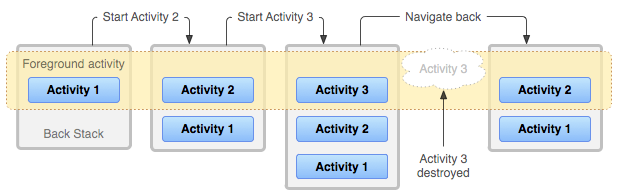
\includegraphics[scale=0.6]{diagram_backstack}

Activity는 스택에 차례대로 쌓인다(Back Stack으로 불린다). 스택은 말 그대로 First In, Last Out 방식으로 쌓이고 사라진다. 스택 구조라서 넣거나 빼기만 할 수 있고 순서를 바꿀 수 없다고 개발자 가이드에 있지만 꼭 그렇진 않다. Intent.FLAG\_ACTIVITY\_REORDER\_TO\_FRONT 플래그를 사용하면 순서를 조정할 수 있다.\\

단순하게 startActivity()를 실행해서 스택에 추가하고 Back 키로 제거해가면 아무 일도 없지만, 실제 앱에서는 다양한 경로의 Activity 접근이 이루어지기 때문에 내비게이션이 꼬이는 경우가 많다. 이 때문에 태스크 관리가 필요하다.

예를 들어보자. 
\begin{enumerate}
\item 캘린더 앱은 달력 화면(A)에서 일정 상세 화면(B)으로 가고 다시 일정 수정 화면(C)으로 이동한다. 그러다가 Home 키를 눌러서 태스크를 백그라운드로 보낸다. 
그런데 홈 스크린 화면에 일정 목록 App Widget이 있어서 특정한 일정으로 이동할 수 있다. 그렇다면 이 특정한 일정 보기 화면은 앞에 있던 A, B, C 위에 B를 추가하면 될까? 아니면 C를 스택에서 없애고, B를 다시 로딩하게 할까?
\item 사진 공유 앱에서 사진 목록 화면(A)에서 등록자의 프로필 이미지를 클릭하면 등록자의 프로필을 포함한 동록자의 사진 목록 화면(B)로 이동한다. B 화면의 사진들에는 ``좋아요''를 한 사용자 이미지들이 있는데 이 이미지를 클릭하면 그 사용자의 사진 목록 화면 B'으로 이동한다. 계속 반복해서 사용자의 사진 목록 화면이 쌓일 수도 있고, 아니면 같은 화면에서 화면만 갱신할 수도 있다. 어느 쪽이 원하는 방식일까?
\end{enumerate}

각 앱에서 원하는 내비게이션 방식이 있는데, 태스크의 동작 방식을 이해하지 못한다면 사용자가 보고자 하는 화면이 아닌 엉뚱한 화면을 접하는 경우가 생긴다. 물론 이해가 간단하지 않고 많은 시행착오가 우리 앞에 기다리고 있다.

\subsection{태스크 상태}
태스크는 화면에 포커스되어 있는 포그라운드 상태와, 화면에 보이지 않는 백그라운드 상태가 있다. 포그라운드에 있는 것은 Home 키를 통해서 언제든 백그라운드로 이동할 수 있다.
백그라운드에 있는 것도 언제든 포그라운드로 이동할 수 있다. 앱 아이콘이나 Shortcut, App Widget, Notification을 통해 새로운 포그라운드 태스크가 될 수도 있다. Home 화면에 나와있는 경우는 Home 화면이 포그라운드 태스크이다.\\

백그라운드에서 포그라운드로 상태를 변경하는 메서드는 Activity에 moveTaskToBack(boolean nonRoot) 메서드가 있다. nonRoot에 true가 들어가면 어느 위치에서건 백그라운드로 이동할 수 있고, false인 경우에는 태스크 루트일 때만 가능하다. 
메서드 시그너처를 보고서 파라미터의 용도를 볼 때마다 헷갈리는 걸 보면 잘 만든 메서드는 아닌 듯 하다. 메서드 시그너처를 moveTaskToBack(boolean onlyRoot) 이런 식으로 바꾸면 좀 낫지 않을까. \\

이제 반대로 백그라운드에서 포그라운드로 상태를 변경하는 메서드는 있을까? 
Activity가 보이지 않는 백그라운드 상태이기 때문에 Activity의 메서드로는 안 된다.
바로 ActivityManager에서 
List$<$ActivityManager.Running\-TaskInfo$>$ getRunningTasks(int maxNum) 메서드를 통해서 가장 최근의 maxNum개를 가져오고 moveTaskToFront(int taskId, int flags) 메서드에 RunningTaskInfo.id를 taskId에 전달하면 된다.\footnote{관련해서 \url{http://bonjwakim.tistory.com/15}를 참고하자.}
% 권한 필요

\subsection{태스크 확인}
눈으로 화면이 바뀌는 것을 기준으로 테스트하면 태스크가 정상적으로 동작하는지 확인하기 어렵다. Back 키로 이전 화면으로 돌아가면 잘 남아있다고 동일한 태스크라고 확신할 수 없다.
예를 들어, 앱에서 startActivity()를 실행해서 브라우저를 열었다면 앱과 브라우저는 한 묶음 같아 보인다. 그런데 과연 동일한 태스크일까? 그렇지 않다. 브라우저는 singeTask launchMode로 되어 있어서 별도의 태스크로 되어 있다.\\

shell에서 dumpsys를 활용해서 태스크를 확인하면서 각 상황을 이해하도록 하자.
adb shell dumpsys activity activities를 실행하거나, adb shell 내에서 dumpsys activity activities를 실행하면 된다. 마지막 옵션인 activities는 줄여서 a로 써도 된다.\\

dumpsys 내용이 많은 경우 한번에 확인하기 어려워서 리다이렉션을 통해 파일로 저장하는 것을 권장한다. adb shell dumpsys activity a  $>$ tasks.txt 와 같이 사용한다. adb shell 내에서도 dumpsys를 할 수 있지만 shell 내에서는 리다이렉션이 되지 않는다.\\

그래도 워낙 내용이 많긴 하다. 해당 앱 관련 내용만 볼 때는 grep 명령어를 활용하자. dumpsys activity a | grep com.example.android.supportv4 이런 식으로 하면 관련 라인만 볼 수 있다. 필자의 경우는 grep을 통해서 일부만 보면 필요한 정보를 빠뜨릴 수 있지 않나 생각해서 잘 안 쓰는 편이었는데, dumpsys 내용에 패키지명이 계속해서 들어가기 때문에 grep을 통해서 보는 편이 낫다.\\

아래는 adb shell dumpsys activity a를 실행한 결과이다. 참고로 안드로이드 버전마다 dumpsys 결과는 다를 수 있다. \ref{sec:dumpsys} 절에서 dumpsys 명령어를 상세히 보기로 한다.
\lstset{basicstyle=\fontfamily{mono}\selectfont\scriptsize}
\begin{lstlisting}[frame=single]
ACTIVITY MANAGER ACTIVITIES (dumpsys activity activities)
  Main stack:
  * TaskRecord{43495e10 #132 A com.example.android.supportv4 U 0}
    numActivities=3 rootWasReset=false userId=0
    affinity=com.example.android.supportv4
    intent={act=android.intent.action.MAIN cat=[android.intent.category.LAUNCHER] 
    flg=0x10000000 cmp=com.example.android.supportv4/.Support4Demos}
    realActivity=com.example.android.supportv4/.Support4Demos
    askedCompatMode=false
    lastThumbnail=android.graphics.Bitmap@42fcd710 lastDescription=null
    lastActiveTime=123128734 (inactive for 36s)
    * Hist #36: ActivityRecord{432c0720 com.example.android.supportv4/.app.FragmentTabs}
        packageName=com.example.android.supportv4 processName=com.example.android.supportv4
        launchedFromUid=10194 userId=0
        app=ProcessRecord{42c11768 18847:com.example.android.supportv4/u0a194}
        Intent { cmp=com.example.android.supportv4/.app.FragmentTabs }
        frontOfTask=false task=TaskRecord{43495e10 #132 A com.example.android.supportv4 U 0}
        taskAffinity=com.example.android.supportv4
        realActivity=com.example.android.supportv4/.app.FragmentTabs
        baseDir=/data/app/com.example.android.supportv4-2.apk
        dataDir=/data/data/com.example.android.supportv4
        stateNotNeeded=false componentSpecified=true isHomeActivity=false
        compat={320dpi always-compat} labelRes=0x7f07002a icon=0x7f020001 theme=0x0
        config={1.15 450mcc5mnc ko_KR sw384dp w384dp h615dp nrml long port finger 
        -keyb/v/h -nav/h s.110fontTypeIndex}
        launchFailed=false haveState=true icicle=Bundle[mParcelledData.dataSize=3540]
        state=STOPPED stopped=true delayedResume=false finishing=false
        keysPaused=false inHistory=true visible=true sleeping=true idle=true
        fullscreen=true noDisplay=false immersive=false launchMode=0
        frozenBeforeDestroy=false thumbnailNeeded=false forceNewConfig=false
        thumbHolder=TaskRecord{43495e10 #132 A com.example.android.supportv4 U 0}
        waitingVisible=false nowVisible=true lastVisibleTime=-1m8s283ms
    * Hist #35: ActivityRecord{42d3e318 com.example.android.supportv4/.Support4Demos}
        packageName=com.example.android.supportv4 processName=com.example.android.supportv4
        launchedFromUid=10194 userId=0
        app=ProcessRecord{42c11768 18847:com.example.android.supportv4/u0a194}
        Intent { cmp=com.example.android.supportv4/.Support4Demos (has extras) }
        frontOfTask=false task=TaskRecord{43495e10 #132 A com.example.android.supportv4 U 0}
        taskAffinity=com.example.android.supportv4
        realActivity=com.example.android.supportv4/.Support4Demos
        baseDir=/data/app/com.example.android.supportv4-2.apk
        dataDir=/data/data/com.example.android.supportv4
        stateNotNeeded=false componentSpecified=true isHomeActivity=false
        compat={320dpi always-compat} labelRes=0x7f070000 icon=0x7f020001 theme=0x0
        config={1.15 450mcc5mnc ko_KR sw384dp w384dp h615dp nrml long port finger 
        -keyb/v/h -nav/h s.110fontTypeIndex}
        launchFailed=false haveState=true icicle=Bundle[mParcelledData.dataSize=1284]
        state=STOPPED stopped=true delayedResume=false finishing=false
        keysPaused=false inHistory=true visible=false sleeping=true idle=true
        fullscreen=true noDisplay=false immersive=false launchMode=0
        frozenBeforeDestroy=false thumbnailNeeded=false forceNewConfig=false
        thumbHolder=TaskRecord{43495e10 #132 A com.example.android.supportv4 U 0}
        waitingVisible=false nowVisible=false lastVisibleTime=-1m13s34ms
    * Hist #34: ActivityRecord{42c07700 com.example.android.supportv4/.Support4Demos}
        packageName=com.example.android.supportv4 processName=com.example.android.supportv4
        launchedFromUid=2000 userId=0
        app=ProcessRecord{42c11768 18847:com.example.android.supportv4/u0a194}
        Intent { act=android.intent.action.MAIN cat=[android.intent.category.LAUNCHER] 
        flg=0x10000000 cmp=com.example.android.supportv4/.Support4Demos }
        frontOfTask=true task=TaskRecord{43495e10 #132 A com.example.android.supportv4 U 0}
        taskAffinity=com.example.android.supportv4
        realActivity=com.example.android.supportv4/.Support4Demos
        baseDir=/data/app/com.example.android.supportv4-2.apk
        dataDir=/data/data/com.example.android.supportv4
        stateNotNeeded=false componentSpecified=true isHomeActivity=false
        compat={320dpi always-compat} labelRes=0x7f070000 icon=0x7f020001 theme=0x0
        config={1.15 450mcc5mnc ko_KR sw384dp w384dp h615dp nrml long port finger 
        -keyb/v/h -nav/h s.110fontTypeIndex}
        launchFailed=false haveState=true icicle=Bundle[mParcelledData.dataSize=1284]
        state=STOPPED stopped=true delayedResume=false finishing=false
        keysPaused=false inHistory=true visible=false sleeping=true idle=true
        fullscreen=true noDisplay=false immersive=false launchMode=0
        frozenBeforeDestroy=false thumbnailNeeded=false forceNewConfig=false
        thumbHolder=TaskRecord{43495e10 #132 A com.example.android.supportv4 U 0}
        waitingVisible=false nowVisible=false lastVisibleTime=-1m21s22ms
  * TaskRecord{43294328 #131 A com.example.android.apis U 0}
        ...
        
  Running activities (most recent first): // (1)
    TaskRecord{43495e10 #132 A com.example.android.supportv4 U 0}
      Run #12: ActivityRecord{432c0720 com.example.android.supportv4/.app.FragmentTabs}
      Run #11: ActivityRecord{42d3e318 com.example.android.supportv4/.Support4Demos}
      Run #10: ActivityRecord{42c07700 com.example.android.supportv4/.Support4Demos}
    TaskRecord{43294328 #131 A com.example.android.apis U 0}
      Run #9: ActivityRecord{42f55e10 com.example.android.apis/.app.FinishAffinity}
	...
 
  mResumedActivity: null
  mFocusedActivity: ActivityRecord{432c0720 com.example.android.supportv4/.app.FragmentTabs} // (2)
  mLastPausedActivity: ActivityRecord{432c0720 com.example.android.supportv4/.app.FragmentTabs}
  mSleepTimeout: false
  mDismissKeyguardOnNextActivity: false

  Recent tasks: // (3)
  * Recent #0: TaskRecord{43495e10 #132 A com.example.android.supportv4 U 0}
    numActivities=3 rootWasReset=false userId=0
    affinity=com.example.android.supportv4
    intent={act=android.intent.action.MAIN cat=[android.intent.category.LAUNCHER] 
    flg=0x10000000 cmp=com.example.android.supportv4/.Support4Demos}
    realActivity=com.example.android.supportv4/.Support4Demos
    askedCompatMode=false
    lastThumbnail=android.graphics.Bitmap@42fcd710 lastDescription=null
    lastActiveTime=123128734 (inactive for 37s)
  * Recent #1: TaskRecord{43294328 #131 A com.example.android.apis U 0}
    numActivities=4 rootWasReset=false userId=0
    affinity=com.example.android.apis
    intent={act=android.intent.action.MAIN cat=[android.intent.category.LAUNCHER] 
    flg=0x10000000 cmp=com.example.android.apis/.ApiDemos}
    realActivity=com.example.android.apis/.ApiDemos
    askedCompatMode=false
    lastThumbnail=android.graphics.Bitmap@42ec86d0 lastDescription=null
    lastActiveTime=123083178 (inactive for 82s)
...

  mCurTask: 132          
\end{lstlisting}
\lstset{basicstyle=\ttfamily\small}
\begin{itemize}
\item 태스크는 최신 것이 먼저 위쪽에 나타난다.
\item TaskRecord 섹션에서는 numActivities와 그 안의 Hist 섹션을 통해 스택을 들여다볼 수 있다. 다양한 설정 데이터도 보여준다. ProcessRecord에는 프로세스명(패키지명) 앞뒤로 프로세스의 PID와 USER ID도 보여준다(adb shell에서 ps 명령어로 확인해보자).
TaskRecord에는 app=null로 나오고, state=DESTROYED로 있는 것도 볼 수 있는데, 프로세스가 종료된 것이다. 아래 쪽으로 가면 하루나 이틀 지난 것까지도 나온다. 말 그대로 히스토리이다. 
\item 79 라인(1)에 Running activities 섹션은 스택의 간략한 내용으로 나온다.
\item 94 라인(3)에 RecentTasks 섹션도 내용이 반복되지만, 태스크의 간략한 개요가 나온다(numActivities 등).
\item 89 라인(2)에 화면에 포커스되어 있는 Activity가 나온다.
\item 마지막 라인에 현재 포그라운드에 있는 태스크를 보여준다. 홈 화면도 하나의 태스크이기 때문에 홈 화면으로 나와있다면 Launcher가 현재 태스크로 보인다.\footnote{시점에 따라 백그라운드의 태스크 번호를 보여주기도 한다. 이 번호는 참고 데이터 정도로만 생각하자.}
\end{itemize}
% 케이스를 좀 더 확인할 수 있을까?
dumpsys 명령어는 개발 중에 현재 포커스된 Activity가 어떤 것인지 확인하는 데도 유용하다.
테스트하면서 여러 Activity를 이동하는데, Activity가 많으면 현재 어느 Activity에 있는지 찾아가는 게 간단치 않다.
이 명령어를 몰랐을 때는 시작 Activity부터 로직을 따라가서 현재 Activity를 찾기도 했다. ApiDemos에서 기능을 테스트해보다 관련 Activity를 찾아서 디렉터리를 뒤져본 기억들은 안드로이드 앱 개발자라면 가지고 있을 것이다.

\subsection{taskAffinity}
Activity에서 startActivity()를 실행하는 게 많지만, 알람 같은 경우 BroadcastReceiver에서 startActivity()를 실행하는 것이 일반적이고 Service 실행 중에 Activity를 시작하는 상황도 있다. Application에서는 드물지만 이벤트를 항상 받기 위해서 Application에 BroacastReceiver를 등록하고 여기서 startActivity()를 실행하는 경우가 있다.
그런데 Activity가 아닌 곳에서 startActivity()를 실행하는 경우에는 앱이 포그라운드에 있을 수도 있지만, 기본적으로 백그라운드에서 실행한다고 가정해야만 한다. Activity 외에 다른 컴포넌트에서 startActivity를 실행하면 아래와 같은 에러를 만날 때가 있다.
\begin{lstlisting}[frame=single]
09-07 08:49:32.314: E/AndroidRuntime(482): Caused by: android.util.AndroidRuntimeException: 
Calling startActivity() from outside of an Activity  context requires 
the FLAG_ACTIVITY_NEW_TASK flag. Is this really what you want?
\end{lstlisting}

에러 메시지에 있는 대로 Intent.FLAG\_ACTIVITY\_NEW\_TASK 플래그를 포함해야 한다.
\begin{lstlisting}[frame=single]
Intent intent = new Intent(context, ScheduleViewerActivity.class);
intent.putExtra(SheduleViewerActivity.CALEDAR_ID, 20);
intent.setFlags(Intent.FLAG_ACTIVITY_NEW_TASK);
context.startActivity(intent);
\end{lstlisting}

해당 앱이 태스크 목록에 이미 있는 경우는 어떨까? 태스크가 새로 하나 생성되면서 ScheduleViewerActivity가 뜨는가 하면 그렇지 않다. 바로 taskAffinity가 동일한 게 있다면 이 태스크 위에 뜨게 된다. 
taskAffinity는 AndroidManifest.xml의 Activity 선언에 android:taskAffinity에 지정할 수 있고 속성이 없다면 디폴트 값은 패키지명이다.
결국 taskAffinity 속성을 선언하지 않은 것끼리는 FLAG\_ACTIVITY\_NEW\_TASK 속성을 쓰더라도 같은 태스크에 있게 된다.
taskAffinity는 보통은 안 쓰는 속성이지만, 내부적으로 이런 게 일어나고 있어서, FLAG\_ACTIVITY\_NEW\_TASK를 써도 새로운 태스크가 생기지 않는 것이다.
별도로 속성을 줄 때는 android:taskAffinity=``:alarm'' 식으로 프로세스 분리할 때처럼 :(clone) 뒤에 구분자를 적는 것을 권장한다.\footnote{com.example.android.lifecycle.another 또는 :another와 같은 형식이 모두 가능하지만  another처럼 단순한 이름을 쓰는 것은 허용되지 않는다.}\\

Activity 선언에 taskAffinity 속성을 따로 주는 경우를 알아보자. 다른 화면들과 독립적인 알람 화면 같은 경우가 그렇다. 
알람 앱에 알람 리스트 화면(AlarmClock), 알람 설정 화면(AlarmSettings), 알람 화면(AlarmAlert)과 같이 3개의 화면이 있다고 하자. 
만일 AlarmAlert 화면에 android:taskAffinity 속성이 따로 없다면 어떻게 될까?
일정 시간이 되어 알람이 떴는데 그 순간에 알람 앱의 태스크가 포그라운드나 백그라운드에 이미 있을 수 있다. 
그러면 AlarmAlert 화면이 뜰 때 백그라운드에 있다면 함께 포그라운드로 올라와서 맨 위에 AlarmAlert 화면이 있을 것이고, 포그라운드에 이미 있었다면 AlarmAlert 화면이 그 위에 추가되어서 포커스될 것이다.
백그라운드에 있던 화면이 딸려 올라오는 것도 동작이 이상하다. 결국 이미 포그라운드에 있던 것처럼 동작하게 된다. Back 키를 누르니 방금 전까지 보이지 않았던 알람 설정 화면이 뜨는 것이다.\\

이런 케이스를 막기 위해서 AlarmAlert의 taskAffinity를 다르게 세팅하면, FLAG\_ACTIVITY\_NEW\_TASK Flags를 추가했을 때 새로운 태스크로 뜨게 되므로 딸려 올라오는 일이 없어진다. 이렇게 되면 태스크가 각각이 되어서 한 앱에서 2개의 태스크를 사용하게 된다.
Home 키를 길러 눌러서 최근 앱 목록을 보면 2개가 떠있는 것을 볼 수 있다. AlermAlert 화면이 최근 앱 목록으로 나오는 것을 방지하기 위해서 AndroidManifest.xml의 AlarmAlert 선언에 android:excludeFromRecents=``true''를 추가하면 알람 기능의 기본 형태를 갖추게 된다.


%https://groups.google.com/forum/#!topic/android-developers/wKwnV1k_96A

\subsection{태스크 속성 부여}
Activity에 태스크 속성을 부여하는 방법에는 2가지가 있다. 속성을 아예 부여하지 않고서 개발할 수 있다면 행복하겠지만, 사용하다 보면 효율적이지 않은 부분이 생긴다.
디폴트는 Activity가 인스턴스가 매번 새로 생성돼서 쌓이는 형태이다.\\
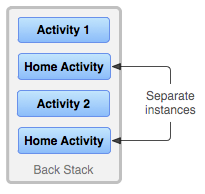
\includegraphics[scale=0.7]{diagram_multiple_instances}\\
속성을 부여하는 2가지 방법은 하나는 불려지는 쪽(Callee )에서 `나를 이런 식으로 취급해줘(존재할거야)'가 있고, 또 하나는 부르는 쪽(Caller)에서 `널 이렇게 다뤄주겠어'하는 것이다. 그리고 2가지 방법의 조합도 있다.
복잡하게 생각할 건 없다. 테스트하면서 원하는 내비게이션 형태를 만드는 과정이 조금 어려울 뿐이다.
아래 설명을 위해서 \url{http://developer.android.com/intl/ko/training/basics/activity-lifecycle/pausing.html}에 있는 ActivityLifecycle.zip을 다운로드하고 변경하면서 테스트해 보자. 
이 샘플에는 ActivityA, ActivityB, ActivityC, DialogActivity(다이얼로그 테마)까지 4개의 Activity가 있다.

\paragraph{Callee 속성 부여는 AndroidManifest.xml의 Activity 선언에 android:launchMode로 한다.}
launchMode에는 standard, singleTop, singleTask, singleInstance 네 가지가 있다. standard와 singleTop은 여러 개의 인스턴스가 존재할 수 있고, singleTask와 singleInstance는 하나의 인스턴스만 존재하다. launchMode 각각을 살펴보자. 설명에서 topActivity(스택의 맨 위)나 baseActivity(스택의 맨 하단)는  ActivityManager.RunningTaskInfo 클래스의 필드명을 그대로 사용했다.
\begin{itemize}
\item standard: 태스크의 topActivity에 매번 새로운 Activity 인스턴스를 생성해서 Intent를 전달한다. Activity의 onCreate() 메서드부터 getIntent() 메서드를 사용할 수 있다.
\item singleTop: 호출하고자 하는 Activity가 이미 topActivity에 있다면 새로 생성하지 않고, onNewIntent() 메서드로 Intent를 전달한다. topActivity에 없을 때는 standard와 동일하게 새로 생성한다.
\item singleTask: 인스턴스는 하나뿐이다. 별도의 태스크로 Activity 인스턴스가 이미 있다면 새로 생성하지 않고, onNewInent() 메서드로 Intent를 전달한다. 
Activity 인스턴스가 없다면 새로운 태스크의 baseActivity로 생성한다. 스택에는 새로운 Activitity를 추가할 수 있다.\\

ActivityLifecycle 샘플에서 ActivityB를 singleTask로 정하고, ActivityA$\rightarrow$ActivityB$\rightarrow$ActivityC 순으로 호출해보자. 하나의 태스크에 모두 쌓이는 것을 볼 수 있다. 바로 taskAffinity가 동일할 때는 아무 의미가 없다. 새로운 태스크로 ActivityB를 띄우려고 하지만 동일한 taskAffinity가 이미 있다면,  ActivityA 위에 그대로 뜨게 된다. 이 내용에 대해서 명시적으로 언급된 부분은 찾지 못했지만 여러 테스트에서도 동일한 결과를 보여 주었다. 이제 ActivityA$\rightarrow$ActivityB$\rightarrow$ActivityC$\rightarrow$ActivityB 순서로 실행해 보자. ActivityC 위에 ActivityB가 올라가진 않고 ActivityC는 스택에서 제거된다. 결과적으로 ActivityA$\Rightarrow$ActivityB 태스크가 남는다. singleTask launchMode의 효과가 전혀 없는 게 아니다.\\

이번에는 ActivityB의 taskAffinity를 변경하고 테스트해 보자. ActivityA$\rightarrow$ActivityB$\rightarrow$ActivityC 순으로 호출하면 ActivityA, ActivityB$\Rightarrow$ActivityC 2개의 태스크가 남게 되다. 
여기서도 ActivityA$\rightarrow$Activi\-tyB$\rightarrow$ActivityC$\rightarrow$ActivityB 순서로 실행해 보자. 역시 ActivityC가 스택에서 제거되고 결국 ActivityA, ActivityB의 2개의 태스크만 남게 된다.\\

앞서 얘기했듯이 모바일 브라우저의 경우가 singleTask launchMode를 사용한다. 
\begin{comment}
http://developer.android.com/intl/ko/training/basics/activity-lifecycle/pausing.html
%이제는 안 그런다..
Facebook에서 기사 링크를 클릭해보면 브라우저가 뜨는데, 이때 dumpsys를 해보면 별도의 Task로 뜨는 것을 확인할 수 있다.\\
이때 홈 키를 길게 눌러서 최근 앱 목록을 확인해보면 Facebook과 브라우저가 각각 따로 보여진다. 당연히 Task가 별개이기 때문에 Facebook을 다시 로딩하면(Recent Apps든, 아이콘을 통해서든), Facebook 화면이 그대로 뜨게 된다.
\end{comment}

\item singleInstance: singleTask와 마찬가지로 인스턴스가 하나뿐이며, 태스크의 유일한 Activity이기도 하다. 여기서 새로운 Activity를 시작하면 이 태스크가 아닌 다른 태스크에 들어가게 되어, 새 태스크를 만드는 효과가 있다. 새 태스크가 되면 새로운 Activity가 뜨는 사이에 검은 화면이 뜨는 시간이 좀 더 오래 걸리는 것을 볼 수 있다. 체감 성능에 차이가 생기므로, 새 태스크가 되어야 하는 케이스와 그렇지 않아도 되는 케이스를 잘 구분하는 것이 좋다.\\

ActivityB의 launchMode가 singleInstance라고 해보자. ActivityA$\rightarrow$ActivityB$\rightarrow$ActivityC 순서로 호출한다고 해보면 재미있는 현상이 발생한다. B는 당연히 하나의 태스크가 된다. 그런데 ActivityA와 ActivityC는 taskAffinity가 동일하기 때문에(ActivityB도 동일하긴 하지만) 하나의 태스크로 다시 묶인다. ActivityC에서 Back 키를 누르면 ActivityB가 아니라 ActivityA로 이동한다. 다시 Back 키를 눌러야만 ActivityB 화면을 볼 수 있다. 즉 결과로 ActivityA$\Rightarrow$ActivityC, ActivityB 태스크가 된다.\\

ActivityA$\rightarrow$ActivityB$\rightarrow$DialogActivity 순서로 호출해보자. 
DialogActivity는 다이얼로그 테마 Activity이므로 배경에 다른 Activity가 있게 되는데, ActivityB에서 DialogActivity를 띄웠으므로 배경에 ActivityB가 있을 것 같지만, 결과는 ActivityA 화면을 배경으로 깔게 된다.
% Level11 이하에서 동작 테스트해봐야 한다.(동일하네?) http://developer.android.com/reference/android/support/v4/app/TaskStackBuilder.html 참고하자. Level 10에서도 emulator에서 동일했다.
여기서 알 수 있는 것은 Activity를 띄우고서 내부적으로 태스크 조정을 하는 것이 아니라 태스크 조정을 하고나서 Activity를 띄운다는 것이다(system\_server 프로세스의 ActivityManagerService에서 태스크를 조정한다). 당연한 얘기인 것 같지만, 이것을 확실하게 알고 있지 않으면 다이얼로그 테마 Activity의 경우처럼 예상치 못한 결과를 볼 수도 있다.\\

최근 앱 목록을 보면 singleInstance로 되어 있는 Activity는 따로 보이지 않는다. 최근 앱 목록도 taskAffinity 기준이라는 것을 알 수 있다.
ActivityB의 taskAffinity를 바꿔주면 어떨까? 결과적으로 태스크가 분리되는 것은 동일하다. 다만 최근 앱 목록에 2개가 따로 뜨는 것을 볼 수 있다.
\end{itemize}
\begin{comment}
singleTask와 singleInstance는 굳이 비유하자면, singleTask는 무조건 새로운 가문을 만들겠다는 것이고, singleInstance는 혼자뿐인 독고다이라고 생각하면 될 듯 하다. 
\end{comment}
singleTask와 singleInstance launchMode는 특별한 상황에서만 사용한다. 사실 태스크 관련 테스트를 하면 제일 혼동되는 게 이 부분이다.

\paragraph{Caller 속성 부여는 Intent Flags에 지정한다.}
Intent에는 setFlags(int flags) 메서드와 addFlags(int flags) 메서드가 있다. 여기에 전달되는 값은 Intent 클래스의 int 상수인 FLAG\_ACTIVITY\_XXX 값이고, 비트 OR 값($|$)으로 여러 개를 전달할 수 있다. 
Intent Flags에 전달하는 값이 Callee의 lanuchMode와 배치되는 경우에는 Callee의 launchMode가 우선한다.\\

Flags에 전달하는 상수는 많다. Caller에서 쓸 수 있는 다양한 옵션이 있는데 그 가운데 주요한 것을 얘기해보자.
\begin{itemize}
\item FLAG\_ACTIVITY\_SINGLE\_TOP: singleTop launchMode와 동일한 효과를 갖는다.
\item FLAG\_ACTIVITY\_NEW\_TASK: singleTask launchMode와 동일한 효과를 갖는다.

\item FLAG\_ACTIVITY\_CLEAR\_TOP: launchMode에 동일한 효과를 갖는 건 없다. 스택에서 Callee보다 위에 있는 Activity들을 종료시킨다. 앞에서 얘기한 달력(A), 일정 상세(B), 일정 수정(C) 화면이 스택상에 있다면, B를 띄울 때 이 플래그를 사용하면 C는 사라지고 B에 원하는 일정을 보여주는 식이다. 보통 FLAG\_ACTIVITY\_SINGLE\_TOP 플래그와 같이 쓰이고, 이때 Callee는 남아있어서 onNewIntent() 메서드에 새로운 Intent가 전달된다. FLAG\_ACTIVITY\_SINGLE\_TOP 플래그를 함께 쓰지 않고 단독으로 쓰이면 Callee는 종료하고서 새로 onCreate()부터 실행된다.
% 단독으로 쓰임: B종료->A종료->A시작->C종료
% 같이 쓰임: B종료->A onNewIntent->C종료
이제 FLAG\_ACTIVITY\_CLEAR\_TOP의 한계도 알고 있어야 한다. ActivityA$\Rightarrow$ActivityB$\Rightarrow$Activi\-tyA$\Rightarrow$ActivityB까지 스택에 있을 때 FLAG\_ACTI\-VITY\_CLEAR\_TOP 플래그를 전달해서 ActivityA를 시작하면 어떻게 될까? 맨 아래에 있는 ActivityA만 남으면 좋겠는데 실제로는 맨 위에 있는 ActivityA 기준으로 ClearTop이 되면서 결과로서 ActivityA$\Rightarrow$ActivityB$\Rightarrow$ActivityA가 스택에 남게 된다. 이를 해결하는 방법으로 \ref{sec:alias} 절에서 <activity-alias>을 활용하는 것을 살펴볼 것이다. 

\item FLAG\_ACTIVITY\_CLEAR\_TASK: Callee가 시작하기 전에 관련한 스택이 모두 제거되고 Callee는 빈 태스크의 baseActivity가 된다. 이 플래그는 FLAG\_ACTIVITY\_NEW\_TASK와 함께 사용되어야 한다. 앱을 사용하면서 태스크에 여러 Activity를 쌓아놓았다가, 로그아웃하고 다른 아이디로 로그인한다면 이 플래그를 사용해서 Launcher Activity를 새로 시작하는 것이 적절할 것이다(허니콤부터 사용).
\item FLAG\_ACTIVITY\_REORDER\_TO\_FRONT: 태스크에 Activity가 있으면 그 Activity를 스택의 맨 위로 올린다. 해당 Activity가 스택에 하나밖에 없어야만 하는 경우에 쓸 수 있다.
그런데 여기서 주의할 게 2가지 있다. 
\begin{itemize}
\item FLAG\_ACTIVITY\_CLEAR\_TOP 플래그와 함께 사용하면 옵션이 무시된다. 
\item Caller가 Activity일 때만 정상적으로 REORDER가 동작한다. FLAG\_ACTIVITY\_NEW\_TASK를 함께 플래그에 사용해야 하는 Service, BroadcastReceiver, Application에서는 FLAG\_ACTIVI\-TY\_RE\-ORDER\_TO\_FRONT가 동작하지 않는다.
\end{itemize}
\end{itemize}

\begin{comment}
이를테면 앱에다 Passcode 기능(해당 앱이 Forground로 올라올 때마다 암호 입력 화면을 먼저 띄우는 기능)을 추가했다고 하면, 앱 최초 실행시나 Background에서 Foreground로 올라올 때에 Passcode 입력 화면이 떠야 한다.\\
Passcode 입력 화면 채로 Home 버튼을 이용해서 Background로 보내버리고, 다음에 알림이나 앱 위젯 같은 것에서 그 Task 위로 다른 Activity A를 띄운다고 하자. 이때도 Foreground로 올라왔으므로, Activity A위에 Passcode 입력 화면이 뜨는 게 맞을 것이다. 그렇다면 여기서 정상적인 암호 입력을 하면 Activity A가 보일 것이고, 여기서 Back 버튼을 누른다면? Task상에 있는 또 다른 Passcode 입력 화면이 뜰 것이다.\\
이런 상황에서 Passcode 입력 화면을 띄울 때, FLAG\_ACTIVITY\_REORDER\_TO\_FRONT을 전달해서 기존에 있던 게 있을때 맨 상위로 올리는 동작을 하면, 이런 상황은 해결된다.\\
\end{comment}

Flags를 쓸 때 제일 중요한 규칙은 가능한 최소한의 플래그만 전달하는 것이다.
진행하는 프로젝트에서 setFlags() 메서드에 5개의 플래그를 조합해서 전달하는 것을 본 적도 있는데, 잘 따져보니 2개만 전달하면 문제가 없는 것이었다.
어떻게든 운이 좋게 원하는 동작에 걸리면 된다는 생각보다는 의도가 명확해야만 한다. 그래야 내비게이션이 변경되어도 문제없이 대응할 수 있다. Callee의 launchMode 속성과 Caller의 Flags를 적절하게 사용해서 조합해야 하는 것은 물론이다. 
% FLAG\_ACTIVITY\_CLEAR\_TOP과 FLAG\_ACTIVITY\_SINGLE\_TOP을 당연히 조합해야 한다고 봐야 하나?

\section{<activity-alias>}\label{sec:alias}
AndroidManifest.xml에는 activity-alias 엘리먼트가 있어서 Activity의 별명을 지정해서 쓸 수 있다. 그런데 별명이 도대체 어디에 도움이 될까?

\begin{comment}
필자의 경우에 처음으로 activity-alias를 적용해 본 경우를 얘기해보자.
해당 케이스는 이렇다.
\begin{itemize}
\item 상세 화면이고 이 화면으로 진입하는 다양한 패스가 있다.
\item 화면을 앱+앱 하이브리드로 변경하려고 한다. 이때 기존 코드는 거의 쓸모가 없기 때문에 아예 다른 Activity로 만들려고 한다. DetailActivty$\rightarrow$DetailWebActivity
\item 테스트 후에 문제가 많다면 원래 상태로 다시 복구하려고 한다.
\end{itemize}

DetailActivity를 호출하는 쪽을 DetailWebActivity로 한꺼번에 바꿔주는 것도 가능하다. 소스 버전 관리툴이 있기 때문에 원복이나 다른 작업자와 충돌 문제가 웬만큼 커버된다.
\end{comment}

\begin{enumerate}
\item 기존에 있던 Activity가 없어졌을 때 사용할 수 있다.
예를 들어, SplashPage가 맨 처음 뜨는 화면이었는데, SplashPage를 제거하고 바로 MainActivity를 보여주기로 했다.
그런데 SplashPage에 대한 링크가 Shortcut과 같이 기존 버전에서 남아있는 경우가 있다.
기존 Shortcut은 이제 MainActivity를 바라보도록 해야 하는데, 이때 쓰는 것이 바로 activity-alias이다.
\begin{lstlisting}[frame=single]
	<activity-alias
    	android:name=".SplashActivity"
        android:targetActivity=".MainActivity">
\end{lstlisting}
android:name에는 반드시 존재하는 클래스명을 넣을 필요는 없다. new Intent(Context packageContext, Class<?> cls)는 결과적으로 new Intent().setComponent(new ComponentName(String pkg, String cls))와 동일하다. 
Shortcut 외에도 PendingIntent.getActivity() 메서드로 알람에 등록되어 링크가 남는 경우도 있다. 대체하는 화면이 존재한다면 activity-alias로 기존 Activity 이름을 남겨두는 것을 고려하자.
\item 앞 절에서 FLAG\_ACTIVITY\_CLEAR\_TOP의 한계를 얘기했다. 동일한 Activity가 태스크에 여러 개 있을 때 이 Activity 또 다시 시작FLAG\_ACTIVITY\_CLEAR\_TOP 플래그를 사용해보자. 이때 맨 아래에 있는 Activity만 남기고 싶지만 맨 위에 있는 것 기준으로 ClearTop이 된다. 이때 쓸 수 있는 방법이 Activity를 처음 시작할 때(즉 맨 아래 Activity에) activity-alias를 사용하는 것이다. 그러면 activity-alias 이름으로  Activity Stack의 맨 아래에 남게 되어서, activity-alias 이름을 기준으로 startActivity()를 실행하면서 FLAG\_ACTIVITY\_CLEAR\_TOP 플래그가 전달되면 원하는 결과를 얻게 된다.
\begin{lstlisting}[frame=single]
	<activity-alias
    	android:name=".FirstActivityA"
        android:targetActivity=".ActivityA">
\end{lstlisting}
\begin{lstlisting}[frame=single]
	Intent intent = new Intent().setComponent(
		new Component(this, "com.suribada.android.FirstActivityA"));
	intent.setFlags(Intent.FLAG_ACTIVITY_CLEAR_TOP 
		| Intent.FLAG_ACTIVITY_SINGLE_TOP);
	startActivity(intent);
\end{lstlisting}
\end{enumerate} 

activity-alias를 쓰면서 제한사항도 있다.
바로 android:targetActivity에 들어가는 Activity는 이전에 선언되어 있어야 한다. 
activity-alias에는 쓸 수 있는 속성이 많지는 않다. 기본 속성은 android:targetActivity를 그대로 따르고 intent-filter는 별도로 쓸 수 있다.

%\begin{comment}
\subsection{윈도우 옵션}
 // No title
\begin{verbatim}
   requestWindowFeature(Window.FEATURE_NO_TITLE);
\end{verbatim}

\begin{itemize}
 \item \verb|FLAG_FULL_SCREEN|: 풀화면을 사용한다. 
\begin{verbatim}
 getWindow().setFlags(WindowManager.LayoutParams.FLAG_FULLSCREEN,  WindowManager.LayoutParams.FLAG_FULLSCREEN); 
\end{verbatim}
 \item \verb|FLAG_SHOW_WHEN_LOCKED|: 스크린이 잠겨있을 때, 윈도우를 보이게 한다. key guard나 다른 lock screen보다 우선순위를 갖게 한다.
스크린을 켜놓기 위해 \verb|FLAG_TURN_SCREEN_ON| 과 함께 쓰일 수 있다. 
\item \verb|FLAG_TURN_SCREEN_ON|: 윈도우가 보여진 다음에는 스크린이 켜진 채로 있게 한다.
\item \verb|FLAG_DISMISS_KEYGUARD|: key gaurd를 없앤다. \verb|<uses-permission android:name="android.permission.DISABLE_KEYGUARD" />| 이 퍼미션 필요하다.
\item \verb|FLAG_TURN_SCREEN_ON|: 스크린을 켠다. 

\end{itemize}

알람 화면 같은 아래처럼 옵션을 사용할 수 있다.
\begin{verbatim}
getWindow().addFlags(WindowManager.LayoutParams.FLAG_SHOW_WHEN_LOCKED
				| WindowManager.LayoutParams.FLAG_KEEP_SCREEN_ON 
				| WindowManager.LayoutParams.FLAG_TURN_SCREEN_ON);
\end{verbatim}		
key guard가 보여지고 있는지 체크한다.
\begin{verbatim}
KeyguardManager keyguardManager = (KeyguardManager)getSystemService(KEYGUARD_SERVICE);
boolean result = keyguardManager.inKeyguardRestrictedInputMode() 
\end{verbatim}


% http://www.androidpub.com/1123549 검토할 것


allowTaskReparenting=["true" | "false"] 디폴트는 false




\end{comment}

\right 
%\subsection{이렇게 해보자.}

\subsubsection{static 메서드로 startActivity를 실행한다.}
\begin{lstlisting}[frame=single]
public class TodoDetailActivity extends FragmentActivity {
	
	private static final String TODO_ID = "todoId";
	private static final String TODO_CONTENT = "content";
	
	private static long todoId = 0L;

	public static void startActivity(Context context, long todoId, String content) {
		Intent intent = new Intent(context, TodoDetailActivity.class);
		intent.putExtra(TODO_ID, todoId);
		intent.putExtra(TODO_CONTENT, content);
		context.startActivity(intent);
	}
\end{lstlisting}
이것은 개발자 가이드에서 Fragment에 Argument를 전달할때 쓰는 방식인데, Activity에서도 활용할만 하다.\\
Intent에 key-value를 전달할 일이 많고, key는 문자열인데, 이 문자열을 Caller와 Callee 양쪽에서 직접 문자열을 넣는 방식은 오타 가능성이 있기 때문에 잘 쓰지 않는다.\\
key를 상수로 갖고 있는 게 좋은데 Caller 쪽에 있는 게 좋을지, Callee 쪽에 있는 게 좋을 지 또 망설여진다. 자주 쓰이는 key라면 별도의 클래스에 상수로 두는 방법도 있겠지만..\\

Callee 쪽에 있다고 한다면, 아래 코드 처럼 된다. 
\begin{lstlisting}[frame=single]
Intent intent = new Intent(this, TodoDetailActivity.class);
intent.putExtra(TodoDetailActivity.TODO_ID, todoId);
intent.putExtra(TodoDetailActivity.TODO_CONTENT, content);
startActivity(intent);
\end{lstlisting}
뭔가 깔끔한 맛이 없다. 이럴 때 Callee 쪽에 static 메서드로 startActivity를 만들어 놓는다면, Caller 쪽에서는 key 값을 신경 쓸 필요가 없고, Callee 쪽에서만 상수를 만들고 이 상수에서 꺼내서 사용하면 된다.\\
전달하는 값이 정해져 있는 경우에 쓸 만한 방법으로 대부분이 이 경우에 해당한다.
그렇지 않을 때는 static  메서드를 너무 많이 만들 수도 없으므로 그럴 때는 Calee 쪽에 상수를 두고서 Calee 쪽에서 참조하는 방법을 그냥 쓰도록 하자.\\

\subsubsection{여러 위젯이 있을 때 동일한 위젯끼리 모아놓는다.}
\begin{lstlisting}[frame=single]
Button okButton, detailButton;
Spinner groupSpinner, statusSpinner;
\end{lstlisting}

\begin{lstlisting}[frame=single]
Button okButton;
Spinner groupSpinner;
Button detailButton;
Spinner statusSpinner;
\end{lstlisting}

Activity에 동작이 많으면 코드가 길어지기 마련이다. 
예를 들어 이벤트 처리시에 ``어떤 스피너를 바꿔야 하지?''할 때가 있는데, 아래 방식보다는 위 방식에서 찾기가 수월하다.\\
AdapterView에서 ViewHolder 패턴을 쓸때도 마찬가지로 동일한 위젯끼리 모아놓는 것이 좋다.
(물론 findViewById() 해서 멤버 변수에 대입하는 것은 레이아웃 순서에 맞게 한다.)\\
동일한 위젯이 많은 때는 Grouping을 다시 할 수도 있다.
\begin{lstlisting}[frame=single]
Button mondayButton, tuesdayButton, wednesdayButton, thursdayButton, fridayButton, saturdayButton, sudayButton;
Button okButton, cancelButton;
\end{lstlisting}

\subsubsection{상수나 멤버 변수는 쓰이는 위치 근처에 선언한다}
무조건 맨 위에다가 멤버 변수를 모두 선언할 필요는 없다. 
메서드 한두개에서만 쓰는 멤버 변수는 바로 그 위에다가 선언해서 변수가 어디에 있고 어디에 쓰이는지 확인하는데 시간을 들이지 않도록 하자.

\subsection{이런거 하지 말자.}

\subsubsection{불필요한 Casting은 하지 말자.}
View나 ViewGroup에 Actvity상에서 기껏해야 Visibility만 조건에 따라 변경되는 경우가 있다. 이럴 때 굳이 findViewById()해서 LinearLayout이니 ImageView니 Casting하는 수고는 하지 말자.\\
% 샘플?
그리고 특히 Layout의 경우에는 변경될 가능성이 아주 많다. 버튼 두개면 LinearLayout 이면 충분한데, 그 버튼 한쪽에 New 마크가 붙는 사소한 이유로 RelativeLayout으로 바뀌어야 할 수가 있다. Layout param 변경이 필요한 경우에만 Casting을 한다.

\subsubsection{상속 구조를 깊게 하지 말자.}
복잡한 앱에서는 액티비티의 상속구조가 4, 5단계까지 있는 것을 본 적도 있다. 이런 코드를 보면, 분석이 상당히 어렵고, 문제가 발생할 때 찾아내는 것에 어려움이 많다.
단순한 유틸리티 메서드를 위해서 상속을 하지는 말자. 로직의 흐름상 반드시 수행해야 할 코드를 중심으로 상위 클래스를 만든다.\\

물론 쉽지는 않다. 클래스 구성을 잘 단순화 해야 하고, 여러 수단을 동원해야만 한다. 내 경우에는 AOP나 Marker Interface 도입 등을 통해서 클래스 구성을 단순화 한 적이 있다. 이 부분에 대해서는 다른 절에서 상세하게 다루기로 하자.\\

\subsubsection{Activity에서 너무 많은 Listener 인터페이스를 구현하지 말자}
OnTouchListener, OnClickListener, OnItemSelectedListener 등 안드로이드에서 제공하는 Listener 인터페이스가 많고, 개발중에도 필요에 의해서 Listener 인터페이스를 만들게 된다.\\

이런 인터페이스들을 Activity 선언에 모두 implements로 해놓고 setOnTouchListener(this), setOnClickListner(this), setOnItemSelectdLister(this) 이런 식으로 하고, 커스텀으로 만든 것까지 하면 여러 개가 될 수가 있다. 이렇게 하면 해당 이벤트의 Listener를 수정할 때, 메서드를 찾아가는 게 간단치 않다. OnClickListener 같은 경우는, onClick 메서드를 찾으면 되지만, OnItemSelectedListener 같은 건 어떨까? Listener에 메서드가 2개이다. 커스텀으로 만든 경우에는 여러 메서드를 가질 수도 있다.\\ 
내가 원하는 메서드를 금방 찾을 수 있을까?\\

이럴 때는 멤버 변수로 Listner 구현을 두는 것으로 전환하는 것도 생각해보자.

\begin{lstlisting}[frame=single]
private OnItemSelectedListener onItemSelectedListener = new OnItemSelectedListener() {

	@Override
	public void onItemSelected(AdapterView<?> parent, View view, int position, long id) {
		....
	}
	
	@Overrides
	public void onNothingSelected(AdapterView<?> parent) {
		...
	}

}	
\end{lstlisting}	
이렇게 하면 setOnItemSelectdLister(this)가 아닌 setOnItemSelectdLister(onItemSelectedListener)를 해놓으면 찾아가는 게 그 전보다 쉬워진다. OnItemSelectedListener의 onNothingSelected()처럼 메서드가 어디에 속한 것인지 익숙하지 않은 것들은 Activity의 메서드로 나와있는 것보다는 위처럼 하는 것을 권장한다.\\

또한 Button 같은 것이 위에서 얘기한 것처럼 Grouping이 되어 있다고 할 때 각각 OnClickListener를 만들어놓는 것이 낫다.
예를 들어 알람설정 화면에 월/화/수/목/금/토/일 같은 요일을 선택하는 Button이 있고, 알람/진동 같은 옵션도 Button으로 있다고 할 때, 같은 OnClickListener를 쓰면 코드를 깔끔하게 만들기 어렵다. 버튼 선택시 다중 선택이  되는 경우도 있고, 하나를 선택하면 다른 것의 선택이 해제되는 동작들 같은 것도 볼 수 있는데, if 문 안에서 번거롭게 처리하는 것보다 그룹별로 따로 Listener를 분리해놓고 생각하자.\\

아래 코드는 5분, 10분, 30분 3개의 버튼 가운데서 하나만 선택되어야 하는 것인데, 다른 Listener하고 분리해서 사용한 예이다.
\begin{lstlisting}[frame=single]
	@Override
	protected void onCreate(Bundle savedInstanceState) {
		...
		mSnoozeFiveMin.setOnClickListener(snoozeListener);
		mSnoozeTenMin.setOnClickListener(snoozeListener);
		mSnoozeThirtyMin.setOnClickListener(snoozeListener);
	}

	private OnClickListener snoozeListener = new OnClickListener() {
		
		@Override
		public void onClick(View view) {
			mSnoozeFiveMin.setSelected(view == mSnoozeFiveMin);
			mSnoozeTenMin.setSelected(view == mSnoozeTenMin);
			mSnoozeThirtyMin.setSelected(view == mSnoozeThirtyMin);
		}
		
	};
\end{lstlisting}	

\begin{comment}
\subsubsection{스레드에서 startActivity를 하지 말자.}
스레드에서 UI 코드가 동작 하지 않는다고 하지만, 그것은 어디까지나 ViewRootImpl의 checkThread를 거치는 경우 뿐이다.(즉 draw/redraw 하는 경우) 스레드에서 startActivity해도 동작은 한다.
\end{comment}
%\section{안드로이드 SDK 도구}

%%android-sdk 아래 platform-tools와 tools 디렉토리가 있다.

\subsection{Hierachy Viewer}
Hierarchy는 타켓 폰에서 기본적으로는 볼 수가 없으므로, emulator를 띄우고, Hierarchy View를 활용한다.
adt가 버전업되면서 문제가 사라졌다.(확인 필요..)

\subsection{adb}
adb 에서 많이 사용하는 명령어가 adb uninstall  패키지명이다.
폰에서 프로그램을 찾아서 uninstall 하는 것보다 빠르다.
안드로이드의 특성상 여러 폰을 가지고 테스트를 하는데, 개발자 여럿이서 동일한 폰을 가지고 테스트하게 된다.
이때 다른 pc에서 올린 것을 가지고 와서 사용할 때 바로 올리진 못하고, uninstall 해야 한다.

adb uninstall com.suribada.notepad

adb install bin/*.apk 명령어는 기존에 앱이 깔려있는 경우에는 쓸 수 없다.
adb install -r [] bin/*.apk 업어쓴다.

emulator를 포함한 여러개의 device를 연결했을 때는, 
adb devices를 통해 기기를 확인할 수 있다.

adb 연결에 문제가 생겼을때 리스타트하는 방법은 다음과 같다.

\begin{verbatim}
adb -s emulator-5554 kill-server
adb -s emulator-5554 start-server
\end{verbatim}

이클립스에서 logcat 결과가 잘 안 보이는 단말기도 있다.
adb devices
adb -s 디바이스명 shell
logcat 해서 볼 수 있다.

adb -e shell(에뮬레이터)
adb -d shell(디바이스)


adb push 디렉토리 /mnt/sdcard 하면 디렉토리의 파일들이 /mnt/sdcard에 올라간다.

바로 실행하기
이게 되려면 Manifest 파일에 등록되어 있어야만 한다.
adb shell am start -n com.nhn.android.search/com.nhn.android.alarmclock.AlarmClock
%http://www.xinotes.org/notes/note/1441/
%http://en.androidwiki.com/wiki/ADB_Shell_Command_Reference 참고하자!
Intent Filter가 없는 경우에는 android:exported="true"가 있어야만, 위 명령어를 쓸 수가 있다.
아니면, java.lang.SecurityException을 발생시킨다.

%http://developer.android.com/guide/topics/manifest/activity-element.html#exported

Shell에 들어가면 /system/bin 아래 사용가능한 메소드들이 보인다. 실제 디바이스에서는 잘 쓰지 못한다.

\section{DDMS}
unKnownHost 문제가 자꾸 나면 emulator를 재시작해보도록 한다.
unknownHostException 나는 경우는 Internet 퍼미션 없을때도 생겨난다.

System.out.println으로 출력하면 Logcat에서는 Tag에 system.out 으로 표시된다.
System.err.println은system.err로 표시된다.

\section{monkey}
크래쉬나, Exception, ANR을 만나면, Monkey가 끝나고 error를 리포트 한다.
% http://blog.daum.net/whisperlip/7287317
파일로 결과를 확인하도록 하자.
\begin{verbatim}
monkey -p com.suribada.notepad -s 269 --pct-touch 50 --pct-nav 5 
--pct-majornav 25 --pct-appswitch 10 --pct-anyevent 10 -v 20000 > /mnt/sdcard/monkey.log
\end{verbatim}


%%\input{intent}

\chapter{Service}
Service를 얘기하기 전에 아래 코드를 한번 보도록 하자. 보통 이렇게 만들지는 않고 다른 클래스를 만들고 그 안에서 스레드를 시작하지만, 결국 아래 형태와 그리 다르지 않다.\\

\begin{lstlisting}[frame=single]
public class LifeCycleApplication extends Application {
	
	private static final long SLEEP_TIME = 10000L;
	
	@Override
	public void onCreate() {
		super.onCreate();
		Log.d("suribada", "Appliction Create");
		Thread thread = new Thread(new Runnable() {

			@Override
			public void run() {
				Log.d("suribada", "Thread start");
				SystemClock.sleep(SLEEP_TIME);
				Log.d("suribada", "10 seconds after");
				SystemClock.sleep(SLEEP_TIME);
				Log.d("suribada", "20 seconds after");
				SystemClock.sleep(SLEEP_TIME);
				Log.d("suribada", "30 seconds after");
			}
			
		});
		thread.start();
		Log.d("suribada", "Appliction Created");
	}

}
\end{lstlisting}

앱이 시작되면서 해야 할 선행 작업들이 있다. 예를 들어, 캘린더 앱이라면 휴일 정보를 업데이트하고 스티커를 다운로드하는 작업이 필요할 것이다. 앱이 시작하면서 Application에서 해야 하는 작업들이니 위 코드는 우리가 가끔 볼 수 있는 코드라고 할 수 있다.\\

시간이 30초나 걸리는 작업이기 때문에 스레드로 뺀 것은 당연하다. 그런데 이건 무슨 문제가 있을까? 
바로 이 앱이 스레드를 마치기 전에 Back 키로 앱을 빠져나오거나, Home 키로 나가서 한참 다른 앱을 사용하느라고 관심을 안 준다면, 프로세스가 종료될 수도 있다는 것이다. 이 스레드가 프로세스 우선순위상 더 진행을 하지 못하고 제거되는 운명에 처한다면 30초나 걸리는 작업의 안정성을 보장할 수 없다.
또는 사용자가 직접 최근 앱 목록에서 제거해버릴 수도 있다. 이때도 프로세스가 종료되면서 스레드도 종료되고 만다. 내부적으로 무엇을 열심히 하고 있는지 사용자가 알 리가 없다.\\

프로세스가 kill될 가능성을 알아보기 위해서, 
\url{http://developer.android.com/guide/components/processes-and-threads.html}를 보고 프로세스의 우선순위를 살펴보자.
\begin{enumerate}
\item Foreground 프로세스: 사용자와 상호작용하는 Activity를 가지고 있거나, 그런 Activity에 bound된 Service를 가지고 있거나, startForeground()를 호출한 foreground Service를 가지고 있거나, Service의 생명주기(onCreate, onStart, onStartCommand, onDestroy)를 실행 중인 Service를 가지고 있거나, onReceive()를 실행하는 BroadcastReceiver를 가지고 있는 경우이다.
메모리가 부족할 때에도 가장 마지막까지 남아 있을 수 있는 프로세스이다.
\item Visible 프로세스: 포그라운드 컴포넌트를 가지고 있지는 않지만, 사용자가 보는 화면에 아직 영향이 있다. Activity로 보면 onPause까지 실행되었지만 visible 상태인 것이다(다이얼로그 테마나 투명한 Activity가 가렸을 때이다).
visible Activity에 bound된 Service를 가진 경우도 해당한다. 
\item Service 프로세스: startService로 실행했지만 위의 카테고리에는 들어가지 않는 Service를 가진 경우이다. 이런 것들은 사용자가 지금 보고 있는 것과 직접적인 연관은 없다.
\item Background 프로세스: 보통 여러 백그라운드 프로세스가 존재한다.
\item Empty 프로세스: 사용자가 Back 키로 종료를 하고 활성화된 컴포넌트가 없다면 Empty 프로세스가 된다. 이런 프로세스를 메모리에 갖고 있는 이유는 다음에 컴포넌트를 띄울때 빠르게 띄우려고 하는 캐시 용도일 뿐이다. 가장 우선순위가 낮아서 리소스가 부족하면 가장 먼저 kill 대상이 된다.
\end{enumerate}

이 우선순위를 보고서 앞에서 제기한 작업의 안정성 문제를 보완할 수 있다. 우선순위상 위 단계로 올라갈 수 있다면 우리는 하려는 작업의 안정성을 보장할 수 있는 것이다. 
위 코드는 아래와 같이 변경할 수 있다. 여기서는 일부러 onCreate() 메서드에서 스레드를 시작하였는데 이후에 다시 살펴볼 것이다.

\begin{lstlisting}[frame=single]
public class LifeCycleApplication extends Application {
		
	@Override
	public void onCreate() {
		super.onCreate();
		Log.d("suribada", "Appliction Create");
		startService(new Intent(this, SleepService.class));
		Log.d("suribada", "Appliction Created");
	}

}
\end{lstlisting}

\begin{lstlisting}[frame=single, caption=SleepService, label=SleepService]
public class SleepService extends Service {

	private static final long SLEEP_TIME = 10000;
	
	@Override
	public void onCreate() {
		Log.d("suribada", "Service onCreate");
		Thread thread = new Thread(new Runnable() {

			@Override
			public void run() {
				Log.d("suribada", "Thread start");
				SystemClock.sleep(SLEEP_TIME);
				Log.d("suribada", "10 seconds after");
				SystemClock.sleep(SLEEP_TIME);
				Log.d("suribada", "20 seconds after");
				SystemClock.sleep(SLEEP_TIME);
				Log.d("suribada", "30 seconds after");
			}
			
		});
		thread.start();
	}
	
	@Override
	public IBinder onBind(Intent intent) {
		return null;
	}

}
\end{lstlisting}
이렇게 하면 일시적으로 가장 우선순위가 높은 Foreground 프로세스까지 갔다가(Service의 생명주기를 실행 중일 때)세 번째인 Service 프로세스에 남아서 작업을 무사히 종료할 수 있는 가능성이 높아진다.
이것은 사용자가 최근 앱 목록에서 제거해도 마찬가지다. 프로세스가 kill되면 서비스는 onStartCommand() 리턴값에 따라 재시작 여부를 결정하는데, 디폴트 리턴값은 START\_STICKY로 Service를 재시작한다.\\

앱이 크래시되는 상황이라면 어떨까? LifeCycleApplication에서 startService()를 실행했는데, 시작 Activity의 onCreate() 메서드에서 크래시로 프로세스가 종료되었다고 하자. 이 경우에도 Service를 시작하기 위해서, LifeCycleApplication을 새로 실행하면서 Service를 시작하는 것을 볼 수 있다.
좀 더 상세하게 살펴보자. 앱 아이콘을 통해서 프로세스가 시작될 때 Application의 onCreate() 메서드에서 startService()를 실행해도, 시작 Activity가 뜨는 것이 먼저 할 작업이기 때문에 Activity가 먼저 시작되고 Service 시작은 그 다음이다.
그런데 시작 Activity의 onCreate() 메서드에서 크래시가 나면, 프로세스는 죽지만 com.android.server.am.ActivityManagerService에서 Pending Service\footnote{Pending Service 목록은 com.android.server.am.ActivityManagerService에서 유지한다. 젤리빈 API 레벨 17 이후에는 com.android.server.am.ActiveServices에서 목록을 유지한다.}를 실행하기 위해서 다시 프로세스를 띄우는데, 이때 Activity는 띄우는 대상이 아니므로 Application을 생성한 이후에 바로 Service가 시작된다.\\

혹자는 Service는 스레드를 안정적으로 돌리기 위한 컴포넌트라고 얘기하기도 한다. 실제 개발에 상당히 유용한 얘기이고 Service에 대한 이해에도 많은 도움을 준다.\\

Service를 언급할 때 자주 나오는 얘기가 백그라운드 상에서 실행되는 컴포넌트라는 것이다. Activity처럼 눈에 보이는 visible 컴포넌트가 아니라는 의미로 백그라운드라는 것으로, 메인 스레드가 아닌 별도 스레드에서 실행하는 것으로 착각하면 안 된다.
Service의 생명주기 메서드 역시 UI 스레드상에서 실행된다. 
따라서 intensive \& blocking 작업을 한다면 Activity에서 UI를 처리하지 못하는 상황이 생길 수 있으므로, Service에서 별도 스레드를 생성해야 하는 경우가 일반적이다.\\

그리고 Service는 해당 앱에서 1개의 인스턴스밖에 생기지 않는다. 따라서 우리는 일부러 싱글톤 객체를 만들고 그 안에서 스레드를 실행할 필요가 없다. 훨씬 안정적으로 동작하는 컴포넌트를 활용하기만 하면 된다.\\

Context에는 Service를 시작하는 방법으로 startService()와 bindService() 메서드 2가지가 있다. 아래 그림은 각각 생명주기 메서드를 구분한 것이다. 

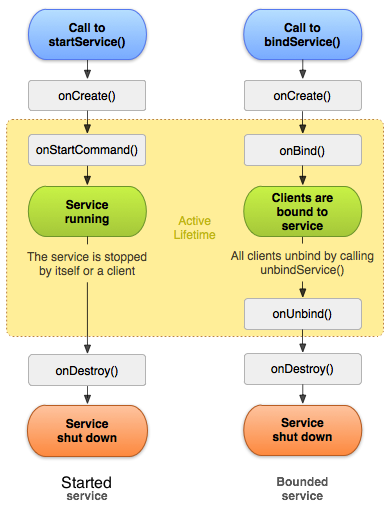
\includegraphics[scale=0.7]{service-lifecycle}

안드로이드 개발자 사이트의 그림에서는 Unbound Service와 Bound Service로 구분하였지만, Unbound Service는 혼동스런 용어이다. Bound되었다가 해제된 것을 의미한다고 오해할 수도 있기 때문에 Unbound Service보다는 Started Service로 부르는 게 더 맞겠다. 이 책에서도 이후 Started Service와 Bound Service로 언급하기로 한다.\\

Service는 보통 Started Service 또는 Bound Service로 존재하는데, Started이면서 Bound일 수도 있다.  Started \& Bound Service는 코드도 좀 더 복잡해지고 고려할 것이 두 배 이상이 되기 때문에 일반적으로 권장되지는 않는다. 가능하면 이런 시나리오는 배제하자.



\section{Started Service}
Started Service는 Context의 startService() 메서드를 통해서 시작된다. 이것 역시 startService()를 호출하는 시점에 Service가 바로 시작되는 것이 아니고, 메인 Looper MessageQueue에 들어가서 메인 스레드를 쓸 수 있는 시점에 Service가 시작된다. startService() 메서드는 곧바로 ComponentName을 리턴하고 다음 라인을 진행한다. startService()는 Intent Bundle에 파라미터를 전달하고 Service에 작업을 하도록 요청해놓는 것 뿐이다.\\

Service는 startService() 메서드를 통해 처음 생성되는 경우에는 onCreate 메서드를 거쳐서 onStartCommand() 메서드를 실행하며, 그 이후에 startService()를 실행할 때면 onCreate() 메서드는 거치지 않고 onStartCommand() 메서드가 실행된다.
onCreate() 메서드 역할은 Service에 필요한 리소스 등을 준비해 놓은 작업을 하고, onStartCommand() 메서드 역할은 이름 그대로 명령을 매번 처리하는 것이다. 그래서 Activity와는 다르게 onCreate() 메서드에는 Intent가 전달되지 않는다.\\

\begin{comment}
쉬운 이해를 위해서, 비유를 들어 얘기해보자.\\
장난감 회사에 홍보 부서를 만들기로 했다.(이것이 Manifest에 등록된 Service이다.). 홍보할 것이 없으면 딱히 할 것도 없이 가만히 있는다. 그러다가 `로보카 폴리 홍보'라는 의뢰가 들어온다.(이것이 startService이다. 의뢰 내용이 Intent이다). 미리 리소스를 준비해놓지 않고 있다가 그제서야 부서를 만들고 복사기나 사무집기 등을 준비한다.(이것을 onCreate라고 봐도 된다.) 그리고서 의뢰 내용을 회의 등을 거쳐서 처리한다.(이것이 onStartCommand 이다). 이제 다른 의뢰가 들어오면 이제는 의뢰 내용만 처리하면 된다.(onStartCommand만 실행한다.)\\
\end{comment}

명령을 던져놓고 Service에서 그 명령을 알아서 실행하는 것에 Started Service를 사용한다고 생각하자.
표준 패턴은 onStartCommand()에서 백그라운드 스레드를 생성해서
백그라운드 상에서 작업을 진행하고, onStartCommand()를 바로 리턴한다. 이런 패턴을 알지 못하고서 필자가 처음 앱을 개발할 때 겪은 문제도 있다. Service에 명령을 보내고서 화면에 작업중이라는 표시의 애니메이션을 실행하고, 작업이 끝나면 애니메이션을 중지하는 기능이다. 
그런데 Service의  onStartCommand() 메서드에서 스레드를 사용하지 않고 작업을 진행해서 메인 스레드를 점유하고 있으니, 역시 메인 스레드를 사용하는 애니메이션이 동작할 리가 없었다. 원리를 이해하면 아무 것도 아니지만 당시에는 당황했던 기억이 있다.\\

Service에서 작업 진행 상황에 따라 Activity에 메시지를 보내려고 한다면 일반적으로 Broadcast를 사용한다.
예를 들어, 서버와 동기화를 하는 SyncService가 있고 화면에서 버튼이나 메뉴로 SyncService를 시작한다. 
동기화를 하는 도중에는 ProgressBar로 `진행중'을 표시하고 동기화가 끝날 때는 ProgressBar를 없애고 종료 메시지를 표시하고자 한다.
이때 Activity에서는 BroadcastReceiver를 등록하고 Service에서는 sendBroadcast()를 실행하는 식이다.\\

또 다른 방식으로는 Intent에 ResultReceiver를 전달하고 Service에서 ResultReceiver에 값을 되돌려줄 수도 있다. 단방향 메시지 전달이라면 이 방식이 간편하다.\\

ResultReceiver 사용 샘플은 아래와 같다. 먼저 Activity의 내용을 보자. 
\begin{lstlisting}[frame=single]
	private View syncLayout, progressBar;
	private TextView syncMessage;

	@Override
	protected void onCreate(Bundle savedInstanceState) {
   		super.onCreate(savedInstanceState);
   		setContentView(R.layout.data_sync);
   		syncLayout = findViewById(R.id.sync_layout);
   		progressBar = findViewById(R.id.progress_bar);
  	 	syncMessage = (TextView) findViewById(R.id.sync_message);
	}

	public void onClickSync(View view) { // (1)
   		syncLayout.setVisibility(View.VISIBLE);
   		progressBar.setVisibility(View.VISIBLE);
   		syncMessage.setText(R.string.sync_progress);

   		Intent intent = new Intent(this, SyncService.class);
   		intent.putExtra(Constant.EXTRA_RECEIVER, resultReceiver); // (2)
   		startService(intent);
	}

	private Handler handler = new Handler();

	private ResultReceiver resultReceiver = new ResultReceiver(handler) { // (3)

   		@Override
   		protected void onReceiveResult(int resultCode, Bundle resultData) {
      		if (resultCode == Constant.SYNC_COMPLETED) { // (4)
         		progressBar.setVisibility(View.GONE);
        		syncMessage.setText(R.string.sync_ended); 
      		}
  		 }

	};	
\end{lstlisting}
\begin{itemize}
\item 13라인(1)의 onClickSync() 메서드가 `동기화' 버튼을 클릭할 때 동작이다. 동기화 관련 레이아웃과 ProgressBar를 visible 상태로 변경하고 텍스트 메시지도  R.string.sync\_progress로 보여준다.
\item 25라인(3)에서 ResultReceiver를 생성하고 ResultReceiver에는 비어 있는 메서드인 onReceiveResult() 메서드를 오버라이드한다. 
\item 29라인(4)에서 SYNC\_COMPLETED resultCode를 받으면 ProgressBar를 감추고 텍스트 메시지는 R.string.sync\_ended로 변경한다. 
\item 25라인(3)의 ResultReceiver 생성자에는 Handler를 넣기도 하고 null로 할 수도 있다. Service의 백그라운드 스레드에서 ResultReceiver의 send() 메시지를 호출하는데, 여기서 UI를 업데이트하기 때문에 Handler를 거쳐 메인 Looper MessageQueue에 넣은 것이다. 호출하는 쪽과 받는 쪽이 둘다 백그라운드 스레드에서 동작한다면 null을 사용해도 된다.
\item 19라인(2)에서 Intent Extra에 ResultReceiver 인스턴스를 전달한다. ResultReceiver는 Parcelable을 구현해서 다른 프로세스 간에도 데이터를 주고받을 수 있는 구조이다.
\end{itemize}

이제 Service에서 ResultReceiver를 사용하는  소스를 보자.
\begin{lstlisting}[frame=single]
	@Override
	public int onStartCommand(Intent intent, int flags, int startId) {
   		new Thread(new Runnable() {
      
      		@Override
     		public void run() {
         		Log.d(TAG, "SyncService started");
         		SystemClock.sleep(10000);
         		final ResultReceiver receiver= intent.getParcelableExtra(Constant.EXTRA_RECEIVER); // (1)
         		receiver.send(Constant.SYNC_COMPLETED, null); // (2)
         		stopSelf();
     		}

   		}).start();
   
   		return START_NOT_STICKY;
	}
\end{lstlisting}	
9라인(1)에서 Intent에서 ResultReceiver를 꺼내오고, 작업을 다한 후에 10라인(2)에서 send() 메서드를 호출해서 SYNC\_COMPLETED라는 결과를 다시 보낸다. 여기서는 메시지를 하나만 보냈지만 작업 진행률이나 실패 메시지와 같은 다양한 결과를 보낼 수 있을 것이다.

\subsection{Service 재시작 방식}
가용 메모리가 낮고 포커스를 갖고 있는 Activity의 시스템 리소스를 복구해야 할 때, 안드로이드 시스템은 Service를 강제 종료시키기도 한다. 
그리고서 가능한 한 빨리 Service를 재시작하는데, 여기서 Started Service를 사용하면서 주의할 부분이 있다.
Service도 우선순위에 따라 언제든지 종료될 수 있는데 시스템이 알아서 재시작한다는 의미에서 Service를 믿고 안정감을 얻을 수도 있지만, 방식을 이해하지 않으면 반복해서 크래시를 맞이할 수도 있다.\\

Started Service에서는 onStartCommand() 메서드에서 리턴하는 int 상수를 가지고서 재시작 방식을 제어한다. onStartCommand() 메서드의 시그너처는 다음과 같다.\\

public int onStartCommand(Intent intent, int flags, int startId)\\

리턴값으로 사용되는 int 상수를 하나씩 살펴보자.\\
\underline{\bfseries START\_NOT\_STICKY} startService()를 통해서 onStartedCommand() 메서드가 리턴된 상태에서 kill 되면 재시작하지 않는다. 명시적으로 startService()를 실행할 때만 의미가 있는 작업에 사용한다.
예를 들어, 화면에 보여줄 뉴스를 네트워크를 통해서 가져와서 저장할 수 있는데, 메모리 이슈로 인해 Service가 kill되었다면 다시 startService() 명령을 기다려서 최신 뉴스를 가져오는 것이 나을 것이다.\\

\underline{\bfseries START\_STICKY} onStartCommand() 메서드의 기본 리턴 값이다. 정상적으로 종료되지 않았을 때 재시작한다. 재시작시에는 다시 onStartCommand()를 호출하는데 이때 Intent 매개변수가 null로 전달된다.
startService()를 실행할 때 Intent에 값을 전달하고 이 값을 startCommand() 메서드에서 사용할 때는 NullPointerException 발생 가능성이 있다. 
전달된 Intent 값을 사용하지 않고 내부적인 상태만을 가지는 Service에 적합하다.
예를 들면 서버 API 에 접근해서 날씨 정보를 가져와서 업데이트하는 것과 같이 지속적인 데이터 동기화 작업이 해당한다.\\

\underline{\bfseries START\_REDELIVER\_INTENT} 재시작하면서 onStartCommand()에 Intent를 다시 전달하여 실행한다. 어떻게든 해당 파라미터를 가지고 실행해야 하는 Service가 이에 해당한다. 쇼핑몰 앱에서 API를 통해서 회사의 상품 목록을 가져온 후 DB에 저장하는 경우를 예로 들 수 있다.\\

재시작 제어 방식도 중요하지만 불필요한 재시작이 발생하는 상황을 없애는 것도 중요하다. 재시작이 안 되려면 정상적인 종료라는 조건이 필요하다. 
Service를 종료하는 방법으로 Context에 stopService() 메서드가 있지만 실제 사용 빈도가 크지 않다. 
앱을 사용하는 내내 실행되는 Service라면 모르지만, 그런 케이스가 많지 않고 권장되는 방식도 아니다. 
Service는 필요할 때만 동작하고 종료하는 것이 좋다.
그럼 Service를 정상 종료하기 위해서 어떤 것을 주로 사용하는가 하면, 바로 Service의 stopSelf() 메서드를 사용한다. 
stopSelf() 메서드는 stopService() 메서드와 역할이 동일하지만 Service 내에서 호출한다는 것이 다를 뿐이다. Service에서 할 일이 다 끝났으면 (백그라운드 스레드든 아니든) stopSelf()를 실행해서 Service를 명시적으로 종료하고 이때 Service는 onDestroy()까지 실행된다.\\

만일 stopSelf()를 실행하지 않은 상태로 계속 남아있다면 어떤 일이 벌어질까. 할 일은 다 끝났는데 Service는 불필요하게 메모리를 차지하고 있고 시작된(started) 상태로 남아있다. 
어느 순간에 메모리 이슈로 Service가 kill되면 리턴 상수가 START\_STICKY나 START\_REDELIVER\_INTENT인 경우에 의도치 않게 재시작하는 일이 생긴다.

\subsection{멀티 스레드 이슈}
Started Service에서 주의할 게 더 있다. 바로 멀티 스레드 이슈이다. 여러 곳에서 startService()를 동시에 호출할 수 있다. 
그래도 어차피 UI 스레드는 단일 스레드 모델이므로, onCreate(), onStartCommand() 메서드는 한번에 하나씩만 호출된다.
그런데 onStartCommand()에서 백그라운드 스레드를 여러 개 동시에 실행할 때, 값을 잘못 공유하면 문제 발생 여지가 생긴다. 앞에서 예를 든 쇼핑몰 앱에서 각 회사마다 API를 통해 상품 정보를 가져오는데, 전달된 Intent의 회사 id를 Service의 멤버 변수로 쓰면 어떤 일이 벌어질까? 바로 엉뚱한 곳에 데이터가 저장되는 상황을 맞게 된다.\\

여러 클라이언트에서 startService()를 실행한다면 각각 작업이 끝났을 때 아직 진행중인 것이 있는지 알 수 없는 경우도 있다. 이때 stopSelf() 메서드를 호출하면 진행중인 작업들에서 문제가 발생한다. 
이 경우에 대비해서 stopSelf() 메서드의 변종인 stopSelfResult(int startId) 메서드가 있다.  startId는 onStartCommand()에서 전달된 값으로 이 startId가 가장 최근에 시작된 것이라면 Service를 종료한다. 이 메서드를 사용하면 각각의 작업이 끝날 때마다 stopSelfResult()를 실행해도 더 안전해진다.

\subsection{암시적 인텐트로 서비스 실행}
Service는 AndroidManifest.xml에 등록할 때 intent-filter를 추가하면 외부에서 접근할 수 있다.
\begin{lstlisting}[frame=single]
<service android:name=".app.RemoteService" android:process=":remote">
	<intent-filter>
		<action android:name="com.example.android.apis.app.REMOTE_SERVICE" />
	</intent-filter>
</service>
\end{lstlisting}

\begin{lstlisting}[frame=single]
ComponentName componentName = startService(new Intent("com.example.android.apis.app.REMOTE_SERVICE"));
\end{lstlisting}
action name이 동일한 Service가 여러 개 있는 경우는 어떨까? 참고로 Activity의 경우는 action name이 동일하면 Activity를 선택하라는 화면을 보여주고, Broadcast는 action name이 동일한 모든 BroadcastReceiver를 실행한다.
Service는 intent-filter의 android:priority 속성값\footnote{\url{http://developer.android.com/guide/topics/manifest/intent-filter-element.html}를 참고하자. priority값은 -999에서 999까지이다. 디폴트값은 0이다. 실제로 범위를 넘는 값을 넣어도 실행에는 문제가 없다. IntentFilter 소스를 봐도 체크 로직이 없다. 가용한 범위도 충분하기 때문에 굳이 범위를 넘어서 쓰진 말자. 이후 버전에서는 유효성 체크에 범위가 사용될 수도 있다.}을 먼저 비교해서 높은 것을 실행하고, android:priority 값이 같은 경우에는 시스템이 랜덤으로 선택해서 실행한다.

\begin{lstlisting}[frame=single]
<service android:name=".app.RemoteService" android:process=":remote">
	<intent-filter android:priority="999">
		<action android:name="com.example.android.apis.app.REMOTE_SERVICE" />
	</intent-filter>
</service>
\end{lstlisting}

intent-filter를 적용하지 않고 외부에서 서비스를 직접 시작할 수도 있다. 바로 명시적 인텐트를 사용하는 것이다.
\begin{lstlisting}[frame=single]
ComponentName cName = new ComponentName("com.example.android.apis", "com.example.android.apis.app.ServiceStartArguments");
startService(new Intent().setComponent(cName));
\end{lstlisting}

여기에는 제약사항이 있다. 바로 AndroidManifest.xml에 android:exported 속성을 true로 줘야 한다.\footnote{android:exported 속성은 false이고 intent-filter가 있다면 디폴트값이 true가 된다.}
\begin{lstlisting}[frame=single]
<service android:name=".app.ServiceStartArguments" android:exported="true" />
\end{lstlisting}

롤리팝부터는 암시적 인텐트로 Service를 시작하면 문제가 발생한다. startService(), bindeService() 둘 다 마찬가지다.
AndroidManifest.xml에 targetSdkVersion을 21이상으로 하면 롤리팝 이상 단말에서 `java.lang.IllegalArgu\-mentException: Service Intent must be explicit'  예외가 발생하고, targetSdkVersion이 그 아래이면 호환 모드로 동작하여 예외가 발생하진 않지만 `W/ContextImpl: Implicit intents with startService are not safe: Intent { act=com.naver.android.sample.SYNC\_SERVICE (has extras) } android.content.ContextWrapper.startService:533 ...'과 같은 로그가 남는다. 
관련해서 코드를 보려면 롤리팝 버전 ContextImpl의 validateServiceIntent() 메서드를 보자. 여기서도 targetSdkVersion을 체크하는 것을 볼 수 있다.\\

만일 클래스명을 알고 있다면 롤리팝에서도 앞에서 ComponentName을 쓴 것처럼 명시적 인텐트를 사용하면 된다.

\subsection{IntentService}
일반적인 앱에서 멀티 스레딩이 필요한 경우가 많지는 않다. 동시에 여러 요청을 처리할 필요가 없다면 IntentService를 활용하자.
IntentService는 내부적으로 1개의 백그라운드 스레드를 두고 전달된 Intent를 순차적으로 처리한다(내부적으로 HandlerThread를 사용한다).\\

IntentService에서는 백그라운드 스레드에서 실행되는 내용인 onHandleIntent(Intent) 메서드만 구현하면 된다.
물론 생성자 문제 때문에 한 가지를 더 해야 한다. 아래와 같이 생성자가 추가되지 않으면 `no empty constructor exception'이 발생한다. 
\begin{lstlisting}[frame=single]
public class NewsReaderService extends IntentService {

	public NewsReaderService() {
		super("NewsReader");
	}

	@Override
	protected void onHandleIntent(Intent intent) {
		...
	}
	
}	
\end{lstlisting}
IntentService에서 내부적으로 구현한 onStartCommand() 메서드는 기본 리턴값은 START\_NOT\_STICKY이다. 이 값을 변경하려면 생성자에서 아래 메서드를 호출하면 된다.\\ 

setIntentRedelivery(true)\\

IntentService를 사용할 때 내부 구조를 이해하지 못하면 생기는 문제가 있다. 
한 예를 들어보자.\\

백그라운드 스레드에서 Toast를 띄우려고 하면, Toast 내부 클래스 TN에서 new Handler()로 Hanlder 생정자를 사용하는 부분이 있어서 Looper가 없다고 에러를 발생시킨다. 그럼 백그라운드 스레드에서 Looper.prepare()를 실행하면 어떤가 하면 Toast를 정상적으로 보여준다.\\

그럼 IntentService의 작업 스레드에서 동작하는 메서드인 onHandleIntent()에서 Toast를 띄운다면 어떨까. 
내부적으로 사용하는 HandlerThread에서 이미 Looper.prepare()가 되어 있기 때문에 Toast가 뜨는 게 문제없어 보이고, 여기서 크래시가 나진 않지만 심각한 오동작이 가끔 발생한다.\\

Toast.show()를 실행하면 Binder 통신을 통해 system\_server 프로세스에서 NotificationManagerService의 enqueToast() 메서드를 호출한다. 이때 파라미터로 Binder Callback(TN 인스턴스)이 전달되고, Callback에서는 화면에 Toast를 보여주는 작업과 일정시간 후에(Toast.LENGTH\_SHORT, Toast.LENGTH\_LONG) 제거하는 작업을 진행한다.\\

그런데 IntentService에서는 onHandleIntent() 실행 이후에 바로 stopSelf()를 호출하고, onDestroy()에서는 HandlerThread에서 생성한 Looper를 종료하는 Looper.quit()을 호출한다. Looper가 종료되면서 생기는 현상은 Looper의 MessageQueue에 전달되는 Callback이 실행되지 않는다는 것이다.
이때 크래시는 나지 않고 로그에 MessageQueue 태그로 Warning이 나온다. `... sending message to a Handler on a dead thread'\\

뜨기로 한 Toast가 안 뜨는 건 해로운 정도는 아니다. 문제는 실행 시점 때문에 Toast는 떴지만, Toast 제거하는 Callback이 불리지 않는 것이다(중간에 Looper가 종료된 것이다).
Toast가 사라지지 않고 내내 남아있는 현상이 발생하는데 심각한 문제다. 그런데 이게 결국 시점 문제라서 재현이 잘 되지도 않는데, 결국 원리를 모르면 해결할 수 없는 문제가 되고 만다.\\

Toast는 가급적 메인 스레드에서만 띄우는 게 맞다. 백그라운드 스레드에서는 그냥 쓰면 크래시가 나기 때문에 결국 안 쓰게 되지만, IntentService에서 아무 고려 없이 `써보니 잘 되네' 하고 넘어가면 안 된다. Looper.getMainLooper()를 통해 메인 스레드에 연결된 Handler를 가지고서 Toast를 띄우는 것이 더 적절하다.
%간단 샘플 필요

\subsection{Service 중복 실행 방지}
코드 \ref{SleepService}에서는 onStartCommand()가 아닌 onCreate() 에서 스레드를 생성해서 작업을 처리하였다. 
이렇게 한 의도는 여러 곳에서 startService()를 실행하는 경우에도 매번 실행하지 않고, 이미 시작되었으면 나머지는 skip하려는 의도를 가지고 만들어 본 것이다.
skip이 필요한 경우를 얘기해 보자. 
메모 앱 같은 경우 시작할 때도 동기화를 실행하고, 버튼을 눌러도 동기화를 실행하고, 메모를 추가했을 때도 동기화를 실행하려고 한다. 
그런데 동기화 작업같은 경우 동시에 여러 개를 실행하면 문제 발생 소지가 있다. 
앱 사용자는 이런 작업이 하나씩 끝날 때까지 대기하는 것이 아니기 때문에, 하다보면 여러 곳에서 시간이 겹친 채로 동기화를 실행할 수 있다.
이때 한가지 작업에만 충실하고 나머지는 확실히 skip해야 하는데, 코드 \ref{SleepService}처럼 onCreate()에서 처리하는 방법도 가능하다. 
onCreate()는 처음 startService()를 호출할 때만 실행하기 때문이다. 
작업이 끝나면 확실히 stopSelf()를 호출한다면 문제가 없다. 다만 Service의 본래 사용 방식과 차이가 있다.\\

IntentService가 skip 용도에 맞는 게 아닐까 하는 생각을 할 수도 있는데, 
IntentService는 백그라운드 스레드 Looper의 MessageQueue에 넣고 순차적으로 하나씩 실행하는 것이므로 이 의도에는 맞지 않다. 여러 번 동기화를 `순차적으로' 실행하는 셈이 된다.\\

onCreate() 메서드가 아닌 onStartCommand() 메서드에서 이런 skip 방식을 적용한 샘플을 보도록 하자.
\begin{lstlisting}[frame=single]
public class SleepThreadService extends Service {

	private static final long SLEEP_TIME = 10000;
	
	private ExecutorService exec = Executors.newSingleThreadExecutor();
	
	@Override
	public void onCreate() {
		Log.d("suribada", "Service onCreate");
	}
	
	private boolean isRunning = false;
	
	@Override
	public int onStartCommand(Intent intent, int flags, int startId) {
		if (isRunning) {
			Log.d("suribada", "skip");
			return START_NOT_STICKY;
		}
		isRunning = true;
		exec.submit(new Runnable() {

			@Override
			public void run() {
				Log.d("suribada", "Thread start");
				SystemClock.sleep(SLEEP_TIME);
				Log.d("suribada", "10 seconds after");
				SystemClock.sleep(SLEEP_TIME);
				Log.d("suribada", "20 seconds after");
				SystemClock.sleep(SLEEP_TIME);
				Log.d("suribada", "30 seconds after");
				stopSelf();
			}
		});
		return START_STICKY;
	}
	
	@Override
	public void onDestroy() {
		isRunning = false;
	}
	
	@Override
	public IBinder onBind(Intent intent) {
		return null;
	}

}
\end{lstlisting}
onStartCommand()는 메인 스레드에서 동작하기 때문에 단순한 boolean 값 가지고 체크가 가능하다.
skip 시에는 START\_NOT\_STICKY를 리턴하는 것도 기억하도록 하자.\\

자바의 concurrency 패키지를 사용한다면 TheadPoolExecutor를 직접 쓰는 방식도 가능하다. 위에서 사용한 Executors.newSingleThreadExecutor() 메서드 같은 정적 메서드는 일반적으로 많이 사용되는 TheadPoolExecutor를 팩토리 메서드로 만든 것이다.\\

ThreadPoolExecutor에 스레드 개수를 1로 고정하면 스레드 풀에 하나의 스레드만 사용하는데, 여기서 중요한 것은 마지막에 추가된 DiscardPolicy이다. 추가로 요청이 들어온다면 버리는 동작을 하는 것이다.
% 만일 이 값이 따로 없다면 crash
\begin{lstlisting}[frame=single]
public class SleepThreadService extends Service {

	....
	
	private ThreadPoolExecutor exec = new ThreadPoolExecutor(1, 1, 0, TimeUnit.SECONDS, 
			new SynchronousQueue<Runnable>(), new ThreadPoolExecutor.DiscardPolicy());
	
	....
		
	@Override
	public int onStartCommand(Intent intent, int flags, int startId) {
		exec.submit(new Runnable() {

			@Override
			public void run() {
				....
				stopSelf();
			}
		});
		return START_STICKY;
	}
	
	....

} 
\end{lstlisting}

\section{Bound Service}
Bound Service는 Service에서 제공하는 메서드를 다른 컴포넌트에서 호출할 수 있게 한 것으로 사용 절차는 간단하다. 먼저 bindService() 메서드를 실행해서 Binding된 이후에 필요한 메서드를 실행한다.\\

Context 클래스에 있는 bindService()의 메서드 시그너처는 아래와 같다.\\
public abstract boolean  bindService (Intent service, ServiceConnection conn, int flags)\\
\begin{itemize}
\item 첫 번째 파라미터인 service는 대상 Service를 가리킨다.
\item 두 번째 파라미터인 conn은 Service에 연결되고 연결이 끊길 때의 Callback이다.
\item 세 번째 파라미터인 flags에는 0을 넣을 수도 있고, Context의 BIND\_XXX 상수를 비트합으로 넣을 수도 있다. ICS부터 추가된 상수들은 주로 Service 프로세스의 우선 순위와 관련된 것이고, 가장 많이 쓰이는 상수는 Context.BIND\_AUTO\_CREATE이다.\\

BIND\_AUTO\_CREATE을 쓸 때만 bindService()를 실행할 때 Service가 없다면 새로 Service를 생성한다. 이 옵션이 없다면 어디선가 startService()를 하지 않았다면 bindService()에서 연결 Callback이 불리지 않게 된다.
즉 Started \& Bound Service가 아니라면 BIND\_AUTO\_CREATE 옵션은 필수적이다. 
이 옵션의 역할은 그 밖에도 더 있다. 
Service에 Binding된 클라이언트가 여러 개 있을 때 stopService()를 실행하면 어떤 일이 발생할까? 이 옵션이 있다면 stopService()를 실행해도 Service가 종료되지 않는데, 옵션이 없는 경우에는 연결이 끊기고서 바로 Service의 onDestroy()가 불린다.
옵션이 있는 경우 unbindService()를 클라이언트마다 모두 실행해야 Service의 onDestroy()가 불린다.
Binding된 Client가 남아 있다면 Service 프로세스가 메모리 문제 등으로 종료되었다가도 다시 Service 프로세스가 살아나나서 재연결되는 것도 이 옵션이 있을 때만 가능한다. 
\end{itemize}

Bound Service의 용도를 이제 생각해보자.
최신 뉴스나 인기검색어, 날씨처럼 업데이트가 필수적인 데이터가 있다. 이런 데이터를 앱에서 쓰는 방법은 어떤 게 있을까?
\begin{enumerate}
\item XML이나 JSON으로 데이터를 리턴하는 API 서버를 만들고, 앱에서 HTTP 호출을 통해 데이터에 접근한다.
\item HTTP 호출을 하고 결과도 객체로 리턴해주는 오픈 API jar를 만들어서, 앱에서는 jar를 이용해서 데이터에 접근한다.
\item 서비스 앱에서 데이터를 제공하는 Bound Service를 만들고(이 안에서 HTTP 호출을 하고 객체를 리턴한다), 다른 앱에서는 bindService()를 실행하여 Service 데이터에 접근한다. 이를테면 검색 앱에서는 인기검색어 목록을 Bound Service로 외부에 제공할 수 있다.
Google Play In-app Billing도 이 방식을 사용하고 있다.
\item bindService()를 실행하고 결과를 받는 것을 래핑한 jar를 만들어서, 다른 앱에서 이 jar를 이용한다. Google Play Services(\url{https://developers.google.com/android/guides/overview})가 이런 형태이다.\footnote{connect()와 disconnect() 메서드가 있는데, bindService()와 unbindService()를 내부적으로 호출해서 사용한다.}
\end{enumerate}
3번과 4번에서 Bound Service를 언급하였다. 
아래로 갈수록 추상화 레벨이 높다. 추상화 레벨이 높은 게 좋은 게 아니라, 현재 시점에 맞는 적절한 방법을 선택하는 게 좋겠다. 오버 엔지니어링을 피하자는 얘기다.\\

Bound Service는 구분해서 로컬 바인딩(Local Binding)과 리모트 바인딩(Remote Binding) 2가지를 얘기한다.
혹자는 뭐하러 Local과 Remote를 구분하느냐고 말하기도 한다.
Remote Binding Service를 만들어도, 로컬에서 호출하면 Binder를 거치지 않고 직접 호출하므로 Local Binding Service가 따로 있을 필요가 없다는 것이다. Remote Binding만으로 커버 가능한데, 사람들이 자꾸 ``그럼 Local Binding은?''하는 문의가 많아서 사실 별 내용이 없는 Local Binding을 별도로 얘기하게 되었다고 한다.\\

\subsection{리모트 바인딩}
Remote Binding Service를 만드는 것이 어렵지는 않다. aidl 인터페이스를 작성한 다음에 Service에서 Stub 인터페이스 구현해주면 된다.
간단한 샘플을 가지고 먼저 알아보자. 
IRemoteService.aidl을 아래와 같이 작성하였다. 
\begin{lstlisting}[frame=single]
interface IRemoteService {

	boolean validCalendar(long calendarId, String calendarType);
		
}
\end{lstlisting}

이렇게 하면 gen 디렉토리에 IRemoteService.java가 생성된다. 아래 코드는 포맷팅을 한 것이고 실제로는 탭이 없이 빽빽하게 붙어있다. 이 소스는 별로 들여다 볼 일은 없지만 한 번쯤은 봐두는 게 좋다.
\begin{lstlisting}[frame=single]
public interface IRemoteService extends android.os.IInterface {
	public static abstract class Stub extends android.os.Binder
			implements com.suribada.calendar.IRemoteService { // (1)
		private static final java.lang.String DESCRIPTOR = "com.suribada.calendar.IRemoteService";

		public Stub() {
			this.attachInterface(this, DESCRIPTOR); // (2)
		}

		public static com.suribada.calendar.IRemoteService asInterface( // (3) 
				android.os.IBinder obj) {
			if ((obj == null)) {
				return null;
			}
			android.os.IInterface iin = obj.queryLocalInterface(DESCRIPTOR); // (4)
			if (((iin != null) && (iin instanceof com.suribada.calendar.IRemoteService))) {
				return ((com.suribada.calendar.IRemoteService) iin);
			}
			return new com.suribada.calendar.IRemoteService.Stub.Proxy(
					obj);
		}

		@Override
		public android.os.IBinder asBinder() {
			return this;
		}

		@Override
		public boolean onTransact(int code, android.os.Parcel data, // (5)
				android.os.Parcel reply, int flags)
				throws android.os.RemoteException {
			switch (code) {
			case INTERFACE_TRANSACTION: {
				reply.writeString(DESCRIPTOR);
				return true;
			}
			case TRANSACTION_validCalendar: {
				data.enforceInterface(DESCRIPTOR);
				long _arg0;
				_arg0 = data.readLong(); // (6)
				java.lang.String _arg1;
				_arg1 = data.readString();
				boolean _result = this.validCalendar(_arg0, _arg1);
				reply.writeNoException();
				reply.writeInt(((_result) ? (1) : (0)));
				return true;
			}
			}
			return super.onTransact(code, data, reply, flags);
		}

		private static class Proxy implements // (7)
				com.suribada.calendar.IRemoteService {
			private android.os.IBinder mRemote;

			Proxy(android.os.IBinder remote) {
				mRemote = remote;
			}

			@Override
			public android.os.IBinder asBinder() {
				return mRemote;
			}

			public java.lang.String getInterfaceDescriptor() {
				return DESCRIPTOR;
			}

			@Override
			public boolean validCalendar(long calendarId,
					java.lang.String calendarType)
					throws android.os.RemoteException {
				android.os.Parcel _data = android.os.Parcel.obtain();
				android.os.Parcel _reply = android.os.Parcel.obtain();
				boolean _result;
				try {
					_data.writeInterfaceToken(DESCRIPTOR); // (8)
					_data.writeLong(calendarId);
					_data.writeString(calendarType);
					mRemote.transact(Stub.TRANSACTION_validCalendar, _data, // (9)
							_reply, 0);
					_reply.readException();
					_result = (0 != _reply.readInt());
				} finally {
					_reply.recycle();
					_data.recycle();
				}
				return _result;
			}
		}

		static final int TRANSACTION_validCalendar = (android.os.IBinder.FIRST_CALL_TRANSACTION + 0);
	}

	public boolean validCalendar(long calendarId, java.lang.String calendarType)
			throws android.os.RemoteException;
}
\end{lstlisting}
\begin{itemize}
\item 52라인(7)의 Proxy와 2라인(1)의 Stub으로 구분되는 클라이언트와 서버는 Parcel을 가지고 데이터를 주고받는다. 
\item 80라인(9)에서 Proxy에서 transact() 메서드를 호출하면 29라인(5)에서 Stub의 onTransact() 메서드가 호출된다.
\item 77라인(8)에서 Parcel에 쓰기 시작하고 40라인(6)에서 읽기 시작한다.
\item 10라인(3)의 asInterface() 메서드 내용을 보자. 7라인(2)에서 attachInterface()에 등록한 것을 15라인(4)의 queryLocalInterface() 메서드로 조회하게 된다. 동일한 프로세스에 있다면 Stub 인스턴스를 직접 사용하겠다는 것이다. 내부적으로 로컬일 수도 있고 리모트일 수도 있는 바인딩이 이때 결정된다.
\end{itemize}

Service에서는 추상 클래스인 Stub 구현체를 만든다.
\begin{lstlisting}[frame=single]
public class RemoteService extends Service {

 	@Override
    public IBinder onBind(Intent intent) {
		return binder;
	}
    	
	private final IRemoteService.Stub binder = new IRemoteService.Stub() {
	
		@Override
        public boolean validCalendar(long calendarId, String calendarType) {
			CalendarType type = CalendarType.vaueOf(calendarType);
            ....
        }
        
    }; 
    
}       	
\end{lstlisting}

다른 컴포넌트에서 Service를 바인딩해서 사용하는 것도 복잡하지는 않다. 
bindService()는 바인딩 결과를 비동기로 받기 때문에, Callback으로 사용할 ServiceConnection 인스턴스를 전달한다.
\begin{lstlisting}[frame=single]
	private IRemoteService mIRemoteService;

	private ServiceConnection mConnection = new ServiceConnection() { // (1)

		@Override
    	public void onServiceConnected(ComponentName className, IBinder service) {
        	mIRemoteService = IRemoteService.Stub.asInterface(service); // (2)
    	}

    	@Override
    	public void onServiceDisconnected(ComponentName className) {
        	mIRemoteService = null; // (3)
    	}
    	
	};

	@Override
	public void onStart() {
		super.start();
		bindService(new Intent(IRemoteService.class.getName()), mConnection, Context.BIND_AUTO_CREATE); // (4)
	}
	
	private void checkValid() {
		if (mIRemoteServer != null) { // (5)
			boolean valid = mIRemoteService.isValidCalendar(10L, CalendarType.NORMAL.name());
			....
		}	
	}
\end{lstlisting}
\begin{itemize}
\item 3라인(1)에서 커넥션 Callback인 ServiceConnection을 생성하였다. 7라인(2)의 Stub.asInterface() 메서드를 통해서 로컬인 경우는 Stub 인스턴스, 리모트인 경우는 Binder Proxy 인스턴스가 mIRemoteService에 대입된다.
어떤 책에서는 ServiceConnection의 onServiceDisconnected()가 Service에서 onUnbind() 된 이후에 호출된다고 잘못 나오기도 하는데, onServiceDisconnected()는 Service에 문제가 생겼을 때(주로 크래시되거나 kill 되었을때) 호출되는 것이다. Service Binding은 아직 유효한 상태이고, 다음에 running 상태가 되면 onServiceConnected()가 알아서 다시 호출된다.
\item 12라인(3)에서 연결이 끊겼을 때는 mIRemoteService를 null로 만든다.
\item 20라인(4)에서 bindService에 ServiceConnection을 전달한다.
\item 24라인(5)에서 Service의 메서드를 호출할 때는 먼저 null을 체크한다. ServiceConnection의 onServiceConnected가 불리기 전일 수도 있고, Service 문제로 바인딩이 안 되었을 수도 있기 때문이다.
\end{itemize}

로컬에서 호출 시에는 호출하는 스레드에서 실행되고, 리모트인 경우에는 Service가 속한 프로세스의 Binder 스레드 풀에서 실행된다. 
스레드 풀에서 실행되기 때문에 Remote Binding Service는 스레드 안전하게 만들어져야만 한다.\\

리모트 바인딩으로 커버 가능하지만 굳이 로컬 바인딩을 얘기하는 이유는 있다. 바로 리모트 바인딩을 지원하려면 Marshaling/Unmarshaling을 해야 하기 때문에 
aidl 인터페이스에 쓸 수 있는 데이터 타입이 제한된다.\footnote{\url{http://developer.android.com/guide/components/aidl.html}을 참고하자.}\\

aidl에서 기본적으로 지원하는 타입을 보자. 
\begin{enumerate}
\item primitive type(int, long, char, boolean 등)
\item String
\item List: 구현체인 ArrayList 같은 건 쓸 수 없다. 제네릭도 조금은 쓸 수 있다. List$<$String$>$, List$<$List$>$ 같은 건 되지만, List$<$?$>$, List$<$List$<$Sting$>>$ 같은 건 안 된다.
\item Map: 역시 구현체인 HashMap 같은 건 쓸 수 없다. 제네릭은 지원하지 않는다.
\end{enumerate}
Serializable 인터페이스 구현 클래스나 enum 같은 건 될 거 같은데 역시 안 된다.
그럼 우리가 만드는 클래스들은 어떻게 지원할까 하면 바로 Parcelable 인터페이스를 구현하면 된다. 
Parcelable로 만들지 않으면 aidl에 import도 되지 않는다(aidl 파일과 동일한 패키지에 있는 클래스도 import 해야 한다).\\

여기에 바로 고민이 생긴다. 전달해야 하는 객체가 복잡하거나 객체의 수가 많다면 이것을 Parcelable로 만드는 것이 만만치 않다.
로컬 바인딩은 이 문제에서 자유롭다. 나도 쓸 수 있고 남도 쓸 수 있게 만들려면 규칙대로(Parcelable) 만들어야 하지만, 혼자서만 쓰겠다면 규칙대로 할 필요가 없는 것이다.\\

\subsection{로컬 바인딩}
로컬 바인딩은 리모트 바인딩보다 간단하게 만들 수 있다.
validCalendar() 메서드에 리모트 바인딩에서는 쓰지 못했던 enum 타입을 파라미터로 전달하는 것도 가능하다. 일반적인 로컬 바인딩 샘플을 보자.
\begin{lstlisting}[frame=single]
public class LocalService extends Service {
	private final IBinder mBinder = new LocalBinder();

	public class LocalBinder extends Binder {
		public LocalService getService() { // (1)
			return LocalService.this;
		}
	}

	@Override
	public IBinder onBind(Intent intent) {
		return mBinder; // (2)
	}
6yj
	public boolean validCalendar(long calendarId, CalendarType calendarType) {
		....
	}

}
\end{lstlisting}
5라인(1)에서 Binder의 원래 메서드가 아닌 getService() 메서드를 추가로 만들고, 12라인(2)에서 LocalBinder 인스턴스를 리턴한다.\\

로컬 바인딩을 사용하는 방법은 리모트 바인딩과 거의 동일하다.
\begin{lstlisting}[frame=single]
public class BindingActivity extends Activity implements OnClickListener {
	private LocalService mService;

	@Override
	protected void onCreate(Bundle savedInstanceState) {
		super.onCreate(savedInstanceState);
		....
	}

	@Override
	protected void onStart() {
		super.onStart();
		Intent intent = new Intent(this, LocalService.class);
		bindService(intent, mConnection, Context.BIND_AUTO_CREATE);
	}
;j'
	@Override
	protected void onStop() {
		if (mService != null) {
			unbindService(mConnection);
		}
		super.onStop();
	}

	@Override
	public void onClick(View view) {
		int id = view.getId();
		if (id == R.id.check) {
			if (mService != null) {
				boolean valid = mService.validCalendar(10L, CalendarType.NORMAL);
				....
			}
		}
		....		
	}

	private ServiceConnection mConnection = new ServiceConnection() {

		@Override
		public void onServiceConnected(ComponentName className, IBinder service) {	
			LocalBinder binder = (LocalBinder) service;
			mService = binder.getService(); // (1)
		}

		@Override
		public void onServiceDisconnected(ComponentName name) {
			mService = null;
		}

	};

	....
	
}
\end{lstlisting}
42라인(1)에서 리모트 바인딩과 달리 onServiceConnected() 메서드에서 결국 얻어내는 것은 LocalService 인스턴스이다.
안드로이드에서 컴포넌트 간에 직접적으로 인스턴스 접근은 가능하지 않는데 Binder 객체를 통해서 직접 접근할 수 있게 한 것이다. 
인스턴스를 얻었으니 그 이후에는 Service의 메서드를 직접 호출하는 방식으로 사용하면 된다. 리모트 바인딩도 사용이 어려운 건 아닌데 로컬 바인딩은 더 간단하다.\\

그런데 여기서 만든 로컬 바인딩 샘플을 보면 뭔가 억지로 끼워 맞춘 느낌이 있다. Service의 메서드를 직접 호출할 수 없으니 바인딩을 통해서 Service 레퍼런스를 가져오고 그 다음은 Service 메서드를 직접 호출하는 것에 불과하다.
리모트 바인딩과 기본 형태도 차이가 있다. 비슷한 형태로 하려면 아래처럼 변경해 볼 수 있다.
먼저 앞에서 IRemoteService.aidl 파일은 그대로 IRemoteService 인터페이스로 만든다.
LocalBinder에서 IRemoteService를 구현한다. Stub을 구현하는 것과 유사하다.
\begin{lstlisting}[frame=single]  
public class LocalService extends Service {
	private final IBinder mBinder = new LocalBinder();

	@Override
	public IBinder onBind(Intent intent) {
		return mBinder;
	}
	
	private class LocalBinder extends Binder implements IRemoteService {

		@Override
		public boolean validCalendar(long calendarId, CalendarType calendarType) {
			....
		}

	}

}
\end{lstlisting}

\begin{lstlisting}[frame=single]
public class BindingActivity extends Activity implements OnClickListener {
	private IRemoteService mService;
	....

	private ServiceConnection mConnection = new ServiceConnection() {

		@Override
		public void onServiceConnected(ComponentName className, IBinder service) {
			mService = (IRemoteService) service;
		}

		@Override
		public void onServiceDisconnected(ComponentName name) {
			mService = null;
		}

	};

	....
	
}
\end{lstlisting}
% 내용 보강
%그래서 Bound Service에서는 ServiceConnection에서 불려지는 메서드에 따라 boolean 값을 바꾸어주거나 Service 참조를 null로 대입해서, 이 값을 if 문에서 한번씩 비교해보고서 Service의 로직을 실행한다.\\

\begin{comment}
\subsection{bindService()를 쓰는 이유}
그래도 ``왜 하필이면 bindService()를 써야 하는가?'' 하는 질문이 있을 수 있다. 한마디로 말하면 bindService()를 통하지 않고서는 Binder\footnote{Remotable object에 대한 기본 인터페이스를 제공한다. android.os.IBinder API 문서를 확인하자.}에 접근할 방법이 없기 때문이다. Service에서 반드시 구현해야 할 메서드인 onBind() 메서드가 리턴하는 것이 IBinder 인터페이스이다.\\

프레임워크 내부에서는 bindService()를 실행하지 않고 ServiceManager에 등록된 Binder 객체를 그대로 가져와서 사용한다.
아래는 ContextImpl 소스의 일부분이다. Stub.asInterface() 메서드를 통해 Stub.Proxy 객체 인스턴스를 얻는다.
\begin{lstlisting}[frame=single]
   static {
   		...
        registerService(ACCOUNT_SERVICE, new ServiceFetcher() {
                public Object createService(ContextImpl ctx) {
                    IBinder b = ServiceManager.getService(ACCOUNT_SERVICE);
                    IAccountManager service = IAccountManager.Stub.asInterface(b);
                    return new AccountManager(ctx, service);
                }});
		...
        registerService(ALARM_SERVICE, new StaticServiceFetcher() {
                public Object createStaticService() {
                    IBinder b = ServiceManager.getService(ALARM_SERVICE);
                    IAlarmManager service = IAlarmManager.Stub.asInterface(b);
                    return new AlarmManager(service);
                }});
		....
	}                
\end{lstlisting}
\end{comment}

\subsection{바인딩의 특성}
\label{subsec:binding_special}
리모트/로컬 바인딩 사용 방법을 얘기했으니, 이제 바인딩의 특성을 더 얘기해보자. 앞에서 얘기한 BIND\_AUTO\_CREATE 옵션에 대해서 다시 한번 언급하는 것이다. 
bindService()를 호출하면 Service와 엮이는 클라이언트가 하나씩 늘어난다고 보면 된다. 
이렇게 엮인 클라이언트가 남아있다면 어느 클라이언트에서 stopService()를 실행해도 종료되지 않는다. 모든 클라이언트가 unbindService() 메서드를 호출해서 Service와의 관계가 모두 정리되어야만 한다.\\
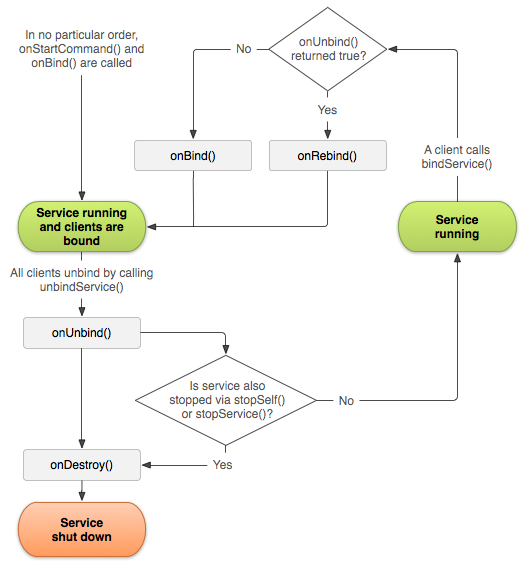
\includegraphics[scale=0.5]{service-binding-tree-lifecycle}\\
이 그림에서 마름모꼴 분기점은 Started \& Bound Service의 경우인데, 앞에서 얘기했듯이 가능하면 생각하지 않는 것이 좋다.\\

기본적으로 Bound Service에서 bindService()를 실행한 클라이언트가 모두 unbindService()를 호출한다면, Service에서는 onUnbind()가 호출되고 onDestroy()까지 호출된다.
Activity에서 Bound Service를 사용할 때는 onStart()와 onStop()에서 bindService()와 unbindService()를 각각 호출하는 것을 권장하고 있다. unbindService()를 실행 시에 연결되어 있는 클라이언트 수가 0가 되면 Service는 종료될 수 있음을 생각해보자. onResume/onPause에서 bind/unbind 하는 경우 onResume/onPause는 빈번하게 트랜지션이 일어나는데(전원 버튼 누르기, 다이얼로그 테마 Activity를 위에 띄우기 등) onPause()를 통해 unbindService()가 실행되고 Service가 종료될 수도 있다. 
그리고서 onResume()에서 다시 시작해야만 한다. 종료된 Service라면 다시 생성하는 비용이 들게 되는데 빈번한 트랜지션에서 계속 생성/종료하는 것은 적합하지 않다.\\

bindService()를 통해 Bound되었으면 이제는 호출하는 쪽과 호출되는 쪽은 클라이언트-서버 관계로 파악하면 된다. 클라이언트에서 메서드를 호출하면 Service에서 결과를 리턴하는 방식이다. 
조회해서 결과를 리턴한다면 떠올려지는 게 바로 ContentProvider이다. 로컬 바인딩은 타입을 자유롭게 쓸 수 있으므로 크게 고민하지 않아도 되겠지만, 리모트 바인딩의 경우는 ContentProvider를 대신 쓸 수도 있다. 물론 DB에서 가져오는 값이 아닐 때는 Cursor 타입으로 리턴하도록 조작해야 한다.\\

얘기가 나온 김에 ContentProvider를 써서 동일한 기능을 만들어보자.
\begin{lstlisting}[frame=single]
	@Override
	public Cursor query(Uri uri, String[] projection, String selection, String[] selectionArgs, String sortOrder) {
		...
		switch (URI_MATCHER.match(uri)) {
			...
			case VALID_CALENDAR:
				return validCalendar(Long.parseLong(selectionArgs[0]),  CalendarType.valueOf(selectionArgs[1]));
				
		}
		throw new IllegalArgumentException("Unknown URI " + uri.toString());
	}

	private Cursor validCalendar(long calendarId, CalendarType calendarType) {
		Calendar calendar = null;
		if (calendarType == CalendarType.NORMAL) {
			...
		} else {
			...
		}
		MatrixCursor cursor = new MatrixCursor(new String[] {"calendar"}); // (1)
		if (calendar != null) {
			cursor.newRow().add("valid");
		}
		return cursor;
	}
\end{lstlisting}
20라인(1)에서 DB Cursor가 아니고 직접 Cursor에 값을 채우는 방법으로 MatrixCursor를 사용하였다.\\

클라이언트에서는 아래와 같이 사용한다.
\begin{lstlisting}[frame=single]
	public boolean isValidCalendar(long calendarId, CalendarType type) {
		Cursor cursor = contentResolver.query(Uri.withAppendedPath(CONTENT_URI, "valid_calendar"), 
				null, null, new String[] {String.valueOf(calendarId), type.name()}, null);
		return (cursor.getCount() > 0);
	}
\end{lstlisting}

Service에서도 작업이 오래 걸린다면 백그라운드 스레드에서 작업을 실행하는 것을 고려할 수 있다. 이때는 네 가지 방법을 고려할 수 있다.
\begin{itemize}
\item 스레드 작업이 끝났을 때 sendBroadcast() 메서드를 통해서 데이터를 전달하거나, 데이터가 많은 경우 다시 클라이언트가 폴링해서 데이터를 가져올 수도 있다.
\item Binder Callback을 메서드에 파라미터로 전달해서 결과를 받는 방법도 있다.\footnote{ApiDemos에서 RemoteService를 참고하자.} 이 방법은 안드로이드 프레임워크에서 많이 쓰이는 방법이다. 앞에 얘기했듯이 Toast.show() 메서드에서도 쓰이고, Activity, Service 등의 컴포넌트 생명주기가 불려지는 것도 system\_server 프로세스의 ActivityManagerService에서 Binder Callback을 통해서 호출된다(ActivityThread의 내부 클래스인 ApplicationThread가 바로 Binder Callback이다).
\item bindService() 메서드의 파라미터인 Intent에 ResultReceiver를 전달하여 Service의 onBind()에서 ResultReciever를 가져오고 작업을 실행하며 결과를 클라이언트에 전달한다.
\item Messenger를 통해서 양방향 통신을 할 수 있다. Messenger도 내부적으로 Binder Callback을 사용하고 있다. Messenger에 대해서는 별도의 절에서 살펴보자.
\end{itemize}

\subsection{Messenger}
\label{subsec:messenger}
Messenger는 Binder Callback을 내부적으로 래핑해서 Bound Service와 클라이언트 간에 Handler로 메시지를 보내고 처리하는 방식을 제공한다.
필자는 수년 간 앱을 개발하면서 Messenger를 사용한 케이스를 몇 번 보지 못했다. 
앞에서 살펴보았듯이 Service와 다른 컴포넌트 간 통신은 다른 옵션으로도 가능하기 때문이다. 
하지만 Messenger를 알아두면 다른 옵션을 복잡하게 사용하지 않아도 된다. 알아두고 필요할 때 활용하도록 하자.\\

먼저 Messenger의 기본적인 내용을 알아보자. 
\begin{itemize}
\item Messenger는 Parcelable 인터페이스를 구현해서 프로세스 간에 전달할 수 있는 객체이다.
\item Messenger에는 2개의 생성자가 있다. Messenger(Handler target)는 Handler를 감싼 것으로 클라이언트와 Bound Service 양쪽에 있다. Messenger(IBinder target)는 Binder Proxy를 생성하는 것으로 클라이언트에 있다.
\item aidl을 내부적으로 사용하는데 IMessenger 인터페이스로 되어 있다. 
이름만으로 보면 Messenger가 IMessenger.Stub을 구현할 것 같은데 그렇지 않고, Handler의 내부 클래스인 MessengerImpl에서 IMessenger.Stub을 구현하고 있다. Stub에서는 Handler의 sendMessage() 메서드를 호출하기만 한다.
\item \ref{sec:messagequeue}절의 Message 소스를 보면 replyTo라는 public 변수가 있다. Handler에 Message를 보내면서 응답을 받을 곳을 replyTo에 지정할 수 있다.
\item Messenger의 send() 메서드는 결과적으로 Binder 통신을 통해 Stub의 메서드를 호출한다. 리모트 통신이기 때문에 send() 메서드는 RemoteException을 던질 수 있다. 
\end{itemize}

%http://developer.android.com/intl/ko/reference/android/app/Service.html
이제 날씨 정보를 업데이트하는 기능을 Messenger로 만들어보자. 요구 사항은 이렇다.
\begin{itemize}
\item 처음 Activity에서 bindService()를 하면, Bound Service에서 날씨 정보를 가져오고 내부에서 주기적으로(예제에서는 1분) 날씨 정보를 가져온다.
\item 날씨 정보를 가져올 때마다 Bound된 Activity에 정보를 전달해서 화면에 보여준다.
\item 추가로 클라이언트가 Bound되면 최신 날씨 정보를 클라이언트에 전달한다.
\item 화면에는 [Refresh] 버튼이 있어서 이 버튼을 클릭하면, 날씨 정보를 새로 가져오고 Bound된 클라이언트 모두에 날씨 정보를 새로 전달한다.
\end{itemize}

Service 코드를 먼저 살펴보자.
\begin{lstlisting}[frame=single]
public class MessengerService extends Service {

	/* input message */
	public static final int MSG_REGISTER_CLIENT = 1;
	public static final int MSG_UNREGISTER_CLIENT = 2;
	public static final int MSG_REFRESH = 3;

	/* output message */
	public static final int MSG_WEATHER = 11;

	public static final String WEATHER_TEXT = "weatherText";
	public static final String TEMPERATURE = "temperature";

	private final ScheduledExecutorService scheduler = Executors.newScheduledThreadPool(1); // (1)

	private ArrayList<Messenger> clients = new ArrayList<>(); // (2)

	private Bundle lastData;

	private class IncomingHandler extends Handler { // (3)

		@Override
		public void handleMessage(Message msg) {
			switch (msg.what) {
				case MSG_REGISTER_CLIENT:
					clients.add(msg.replyTo); // (4)
					if (lastData != null) { // (5)
						Message message = Message.obtain(null, MSG_WEATHER);
						message.setData(lastData);
						try {
							msg.replyTo.send(message);
						} catch (RemoteException e) {
						}
					}
					break;
				case MSG_UNREGISTER_CLIENT:
					clients.remove(msg.replyTo); // (6)
					break;
				case MSG_REFRESH:
					scheduledFuture.cancel(true); // (7)
					fetchWeather();
					break;
				default:
					super.handleMessage(msg);
			}
		}

	}

	private Messenger messenger = new Messenger(new IncomingHandler()); // (8)
	private ScheduledFuture scheduledFuture;

	@Override
	public void onCreate() {
		super.onCreate();
		fetchWeather(); // (9)
	}

	private void fetchWeather() {
		scheduledFuture = scheduler.scheduleAtFixedRate(new Runnable() {

				@Override
				public void run() { // (10)
					Weather weather = callWeatherAPI(); // HTTP Call
					Message message = Message.obtain(null, MSG_WEATHER);
					Bundle bundle = message.getData();
					bundle.putString(WEATHER_TEXT, weather.weatherText]);
					bundle.putInt(TEMPERATURE, weather.temparature));

					lastData = new Bundle(bundle); // (11)
					for (int i = clients.size() - 1; i >= 0; i--) {
						try {
							clients.get(i).send(message);
						} catch (RemoteException e) {
							clients.remove(i); // (12)
						}
					}
				}

			}, 0, 1, TimeUnit.MINUTES); // (13)
	}

	@Override
	public IBinder onBind(Intent intent) { // (14)
		return messenger.getBinder();
	}

}
\end{lstlisting}
\begin{itemize}
\item 4$\sim$6라인은 클라이언트에서 들어오는 Message의 what에 해당하는 값이고, 9라인은 클라이언트에 보내는 Message의 what에 해당하는 값이다.
\item 56라인(9)에서 바로 날씨 정보를 가져온다. 첫 번째 클라이언트가 bindService()를 호출하면 이때 onCreate()가 호출되고 곧바로 날씨 정보를 가져오겠다는 의미이다.
\item 14라인(1)에서 스레드 개수가 1개인 ScheduledThreadPoolExecutor을 생성한다. 80라인(13)의 파라미터를 보면 즉시 태스크를 실행하고 그 이후에는 1분마다 실행한다.
\item 16라인(2)에서 클라이언트 Messenger 목록을 clients 변수에 유지한다.
\item 20라인(3)의 Handler는 클라이언트에서 들어오는 Message를 처리하는 용도이다.
\item 50라인(8)에서 Handler를 감싼 Messenger를 생성하고, 이것을 84라인(14)의 onBind() 메서드에서 messenger.getBinder()로 클라이언트에 전달한다.
\item 26라인(4)에서 MSG\_REGISTER\_CLIENT 값이 들어오면 replyTo에 전달되는 Messenger를 클라이언트 목록에 추가한다.
\item 63라인(10)의 Runnable Task에서는 날씨 정보를 가져와서 Bundle에 담고서 클라이언트 목록에 send() 메서드로 전달한다. foreach 문을 사용하지 않고 인덱스가 높은 숫자부터 쓴 이유는 클라이언트가 dead 상태인 경우에 RemoteException이 발생하는데 75라인(12)에서 클라이언트 목록에서 해당 클라이언트를 제거해도 문제가 없게 하려는 것이다.
\item 70라인(11)에 lastData에 최신 값을 저장하고서, 27라인(5)에서 이 값이 있다면 새로 등록한 클라이언트에 전달한다. 이 방식을 사용하는 이유는 아직 갱신주기가 되지 않은 경우, 최대 1분동안 새로 Bound된 클라이언트에서는 날씨 정보를 전달받을 수 없기 때문이다.
\item 37라인(6)에서 MSG\_UNREGISTER\_CLIENT 값이 들어오면 클라이언트 목록에서 제거한다.
\item 40라인(7)에서 MSG\_REFRESH 값이 들어오면 기존 ScheduleFuture를 취소하고 새로 날씨 정보를 가져온다.
\end{itemize}

이제 클라이언트 코드를 보자.
\begin{lstlisting}[frame=single]
public class MessengerActivity extends Activity {

	private class IncomingHandler extends Handler { // (1)
		@Override
		public void handleMessage(Message msg) {
			switch (msg.what) {
				case MessengerService.MSG_WEATHER:
					Bundle bundle = msg.getData();
					weather.setText(bundle.getString(MessengerService.WEATHER_TEXT) + ", Temparature: " + bundle.getInt(MessengerService.TEMPERATURE));
					break;
				default:
					super.handleMessage(msg);
			}
		}
	}

	private Messenger outMessenger;

	private ServiceConnection serviceConnection = new ServiceConnection() {

		@Override
		public void onServiceConnected(ComponentName className, IBinder service) { // (2)
			outMessenger = new Messenger(service);
			try {
				Message msg = Message.obtain(null, MessengerService.MSG_REGISTER_CLIENT);
				msg.replyTo = inMessenger;
				outMessenger.send(msg); // (3)
			} catch (RemoteException e) {
			}
			Toast.makeText(MessengerActivity.this, "Connected.", Toast.LENGTH_SHORT).show();
		}

		@Override
		public void onServiceDisconnected(ComponentName className) {
			outMessenger = null;
			Toast.makeText(MessengerActivity.this, "Disconnected.", Toast.LENGTH_SHORT).show();
		}

	};

	private Messenger inMessenger = new Messenger(new IncomingHandler()); // (4)

	private TextView weather;

	@Override
	protected void onCreate(Bundle savedInstanceState) {
		super.onCreate(savedInstanceState);
		setContentView(R.layout.two_buttons);
		weather = (TextView) findViewById(R.id.title);
	}

	@Override
	protected void onStart() {
		super.onStart();
		bindService(new Intent(this, MessengerService.class), serviceConnection, Context.BIND_AUTO_CREATE);
	}

	@Override
	protected void onStop() {
		super.onStop();
		if (outMessenger != null) {
			try {
				Message msg = Message.obtain(null, MessengerService.MSG_UNREGISTER_CLIENT);
				msg.replyTo = inMessenger;
				outMessenger.send(msg);
			} catch (RemoteException e) {
			}
		}
		unbindService(serviceConnection);
	}

	public void onClickRefresh(View view) { // (5)
		Toast.makeText(MessengerActivity.this, "Refresh.", Toast.LENGTH_SHORT).show();
		if (outMessenger != null) {
			try {
				Message msg = Message.obtain(null, MessengerService.MSG_REFRESH);
				msg.replyTo = inMessenger;
				outMessenger.send(msg);
			} catch (RemoteException e) {
			}
		}
	}

}
\end{lstlisting}
\begin{itemize}
\item \ref{subsec:binding_special}절에서 얘기한 가이드대로 onStart()와 onStop() 메서드에서 bindService()와 unbindService() 메서드를 호출한다.
\item 3라인(1)의 Handler는 클라이언트에 전달되는 Message를 처리하는 용도이다. 이것을 감싼 Messenger를 41라인에서(4) outMessenger로 생성한다.
\item 22라인(2)의 onServiceConnnected() 콜백 안에서는 IBinder를 감싼 Messenger를 생성하고 replyTo에는 inMessenger를 대입해서 27라인(3)에서 Service에 등록하라는 Message를  보낸다.
\item 72라인(5)은 [Refresh] 버튼을 클릭할 때 동작이다. Service에 날씨 정보를 갱신하라는 Message를 보낸다.
\end{itemize}

이 샘플을 통해 Bound Service를 사용하는 한 가지 장점을 알 수 있다. 각 클라이언트에서 네트워크를 통한 API 호출을 매번 하지 않고 Service 한 곳에서만 네트워크 통신을 하고 모든 클라이언트에 결과를 반영할 수 있는 구조가 가능하다. 샘플처럼  Messenger를 이용하면 더 단순해진다.
% http://wikiware-textcube.blogspot.com/2009/12/4-%EC%95%88%EB%93%9C%EB%A1%9C%EC%9D%B4%EB%93%9C-%EC%96%B4%ED%94%8C%EB%A6%AC%EC%BC%80%EC%9D%B4%EC%85%98-%EA%B8%B0%EC%B4%88.html

\chapter{ContentProvider}
\section{SQLite}\label{sec:sqlite}
SQLite는 로컬 DB이지만 속도가 그렇게 빠르지는 않다. 딱 혼자서 쓸 수 있는 정도라고 생각하자.
SQLite는 네이티브 라이브러리에 포함되어 있고 프레임워크를 통해서 접근하고 사용한다.\footnote{안드로이드 프레임워크에서 사용하는 네이티브 메서드는 jni를 이용해서 /frameworks/base/core/jni/android\_database\_SQLiteConnection.cpp 소스에 연결된다.
안드로이드와 SQLite를 연결해주는 것은 /external/sqlite/android/sqlite3\_android.cpp이고,
안드로이드에 들어가는 SQLite 소스는 /external/sqlite/dist/ 디렉터리에 있다. 여기서 주로 sqlite3.c를 보면 된다.}\\

SQLite db 파일은 /data/data/패키지/databases에 저장된다. 
단말에서는 일반적으로 db 파일에 직접 접근하거나 쿼리를 실행할 수 없다(루팅한 것이 아니라면).\footnote{http://stackoverflow.com/questions/9997976/android-pulling-sqlite-database-android-device를 참고해서 단말에서 db 파일을 가져오는 방법도 알아보자.}\\

개발 시에 에뮬레이터에서 db를 확인하는 방법으로는 2가지를 사용한다.
\begin{itemize}
\item shell을 통해서 쿼리를 실행한다.
\item adb pull을 통해 db 파일을 가져와서, SQLite Database Browser 같은 툴로 데이터를 확인하고 쿼리를 실행한다.
\end{itemize}

adb shell에서 모든 db 파일 목록을 아래 명령으로 확인할 수 있다. *를 넣어서 모든 패키지를 조회 대상으로 했다. 
\begin{lstlisting}[frame=single]
 ls -R /data/data/*/databases 
\end{lstlisting}

\begin{lstlisting}[frame=single] 
/data/data/com.android.browser/databases:
autofill.db
autofill.db-journal
browser2.db
browser2.db-shm
browser2.db-wal
webview.db
webview.db-journal
webviewCookiesChromium.db
webviewCookiesChromiumPrivate.db

/data/data/com.android.deskclock/databases:
alarms.db
alarms.db-journal

/data/data/com.android.email/databases:
EmailProvider.db
EmailProvider.db-journal
EmailProviderBackup.db
EmailProviderBackup.db-journal
EmailProviderBody.db
webview.db
webview.db-journal
webviewCookiesChromium.db
webviewCookiesChromiumPrivate.db

/data/data/com.android.inputmethod.latin/databases:
userbigram_dict.db
userbigram_dict.db-journal

/data/data/com.android.keychain/databases:
grants.db
grants.db-journal

/data/data/com.android.launcher/databases:
launcher.db
launcher.db-journal

/data/data/com.android.providers.calendar/databases:
calendar.db
calendar.db-journal

/data/data/com.android.providers.contacts/databases:
contacts2.db
contacts2.db-journal
profile.db
profile.db-journal

/data/data/com.android.providers.downloads/databases:
downloads.db
downloads.db-journal

/data/data/com.android.providers.media/databases:
external.db
external.db-shm
external.db-wal
internal.db
internal.db-shm
internal.db-wal

/data/data/com.android.providers.settings/databases:
settings.db
settings.db-shm
settings.db-wal

/data/data/com.android.providers.telephony/databases:
mmssms.db
mmssms.db-journal
telephony.db
telephony.db-journal

/data/data/com.android.providers.userdictionary/databases:
user_dict.db
user_dict.db-journal
\end{lstlisting}
별게 아닌 명령어지만 한번쯤 실행해 볼 필요는 있다. 
단말에 깔린 기본 앱(캘린더, 주소록 등)은 기본적으로 ContentProvider를 제공하고, 다른 일반 앱에서 필요한 내용들(미디어 데이터, 시스템 설정 등)도 ContentProvider를 제공하고 있다.
\footnote{안드로이드에서 제공하는 ContentProvider는 android.provider 패키지(\url{http://developer.android.com/reference/android/provider/package-summary.html})에서 확인할 수 있다.}\\

위에서 db 파일 목록을 보면 db 확장자 외에도 db에 -journal이나 -wal, -shm이 붙은 파일이 있는 것을 볼 수 있다.
이것은 바로 SQLite에서 트랜잭션(atomic comit and rollback)을 구현한 방식에 따른 것인데, 디폴트는 rollback-journal(-journal 파일 사용)이고 다른 옵션으로 Write-Ahread Log(보통 WAL이라 쓰고, -wal과 -shm 파일 사용)이 있다.
WAL 방식은 SQLite 3.7 버전부터 시작되었고 젤리빈부터 사용 가능하다.\\ 
%Transaction mode에 대한 설명은 일단 뒤로 미뤄둔다.\\
% 기본 내용 정리. WAL 지원 버전

시스템 설정은 어떻게 테이블이 구성되었는지 확인하기 위해 sqlite shell에 접근해보자.
\begin{lstlisting}[frame=single] 
sqlite3 /data/data/com.android.providers.settings/databases/settings.db
\end{lstlisting}

sqlite shell에서는 SQLite dot command라고 불리는 명령어 모음이 있다.
말 그대로 dot(.)으로 시작하고 다른 명령어처럼 semi-clone(;)을 쓰지는 않는다. 이 명령어 모음은 약 30여 개가 되는데 단순 확인 용도이고 실제 사용하는 명령어는 몇 개 되지 않는다.
.help로 명령어 목록을 보고 필요할 때 더 많은 기능을 활용해보자.
sqlite shell을 끝내는 명령어는 .quit와 .exit 둘 다 사용한다.
\begin{itemize}
\item 테이블 목록 보기
\begin{lstlisting}[frame=single] 
sqlite> .tables       
android_metadata   bookmarks          system           
bluetooth_devices  secure       
\end{lstlisting}

\item 스키마 확인
\begin{lstlisting}[frame=single] 
sqlite> .schema system
CREATE TABLE system (_id INTEGER PRIMARY KEY AUTOINCREMENT,
name TEXT UNIQUE ON CONFLICT REPLACE,value TEXT);
CREATE INDEX systemIndex1 ON system (name);
\end{lstlisting}

\item 조회할 때 칼럼명 헤더를 볼 것인지 옵션. on/off 지정하고 디폴트는 off
\begin{lstlisting}[frame=single] 
sqlite> .headers on 
\end{lstlisting}
\end{itemize}

sqlite shell에서 다양한 데이터베이스 명령어를 실행할 수 있다. 계속해서 system 테이블을 조회해보자.
\begin{lstlisting}[frame=single] 
sqlite> select * from system;
_id|name|value
1|volume_music|11
2|volume_ring|5
3|volume_system|7
4|volume_voice|4
5|volume_alarm|6
6|volume_notification|5
7|volume_bluetooth_sco|7
8|mode_ringer|2
9|mode_ringer_streams_affected|166
10|mute_streams_affected|46
11|vibrate_when_ringing|0
12|dim_screen|1
13|stay_on_while_plugged_in|1
14|screen_off_timeout|60000
15|emergency_tone|0
16|call_auto_retry|0
17|dtmf_tone_type|0
18|hearing_aid|0
19|tty_mode|0
20|airplane_mode_on|0
...
\end{lstlisting}
이 값들은 시스템의 환경 설정 값들이다. 이 조회 결과를 보면 Settings.System 클래스(\url{http://developer.android.com/reference/android/provider/Settings.System.html})에서 사용하는 것을 포함하고 있다. 
Settings.System의 문자열 상수를 보면 이 테이블의 name 칼럼에 있는 값과 동일하다.\\

여기서 value 값을 바꿔줄 수 있을까? Settings.System를 통하면 가능하다.
먼저 아래와 같이 AndroidManifest.xml에 퍼미션을 추가한다(마시멜로에서는 특별한 퍼미션이 되어서 퍼미션을 추가하는 것만으로는 안된다).
\begin{lstlisting}[frame=single]
<uses-permission android:name="android.permission.WRITE_SETTINGS" />
\end{lstlisting}

코드에서는 아래와 같이 값을 변경할 수 있다.
\begin{lstlisting}[frame=single]
Settings.System.putInt(getContentResolver(), Settings.System.AIRPLANE_MODE_ON, 1);
\end{lstlisting}

그런데 이 코드는 단말에서는 보안상 막아 놓는다. 엉뚱한 앱에서 자꾸 비행기 모드로 변경한다면 단말을 도저히 사용할 수 없을 것이다.
이 내용이 에뮬레이터에서는 잘 동작한다.
Settings.System 클래스를 보고 내부적으로 db를 사용하고 있는 것을 알면, 여러 앱에서 사용 가능한 nonsecure \& public 값들을 추가로 넣을 수 있지 않을까? 예를 들어, 가장 최근 검색어를 여러 앱에서 공유할 수도 있다.
아래 코드는 마시멜로 이전 버전의 단말에서 잘 동작한다. \\
\begin{lstlisting}[frame=single]
Settings.System.putString(context.getContentResolver(), "most_recent_keyword",
	"Hawaii");
Settings.System.getString(context.getContentResolver(), "most_recent_keyword");
\end{lstlisting}

단말에서는 AIRPLANE\_MODE\_ON 같은 특정 키에 대해서 업데이트를 막아놓은 것으로 해석하면 된다.\\


sqlite shell에서 쓸 수 있는 명령어 모음은 아래 사이트를 참고하자. 두 번째 사이트가 정리가 잘 되어 있다.
\begin{itemize}
\item http://www.sqlite.org/lang.html
\item http://www.tutorialspoint.com/sqlite/
\end{itemize}


%INSERT OR REPLACE 구문이 있다. PK가 같이 쓰여야 한다.

일반적인 용도에서는 필요없지만, 알면 유용한 게 바로 PRAGMA 명령어이다. PRAGMA는 DB의 환경 변수나 상태 플래그를 가져오거나 변경할 때 사용한다.
SQLiteDatabase 클래스에서 getVersion() 메서드가 있는데 아래 명령어의 결과를 가져온 것이다. 
\begin{lstlisting}[frame=single]
PRAGMA user_version; 
\end{lstlisting}

SQLite 언어 지원에서 C API 등을 보면 다양한 함수가 있는데, 안드로이드의 SQLiteDatabase 클래스에서는 쓸 수 있는 게 많지 않다.
그나마 여기에 도움을 주는 것이 PRAGMA 명령어라고 보면 된다. PRAGMA 명령어를 써서 앱의 환경에 맞는 튜닝도 약간은 가능하다.\\
%PRAGRMA 몇 가지 보여주자.


\subsection{DB Lock 문제}
앱에서 SQLite를 사용하면서 가장 문제가 되는 것은 DB Lock이다.
간단한 key-value라면 메인 스레드에서 쿼리를 해도 별 문제가 없지만, 일반적으로 DB 명령은 백그라운드 스레드에서 실행하는 것이 권장된다. 
DB Lock 문제는 바로 스레드 간(또는 프로세스 간) 명령을 실행하면서 Lock을 잡는 시점이 겹치면서 발생한다.\\

Lock의 기본 내용은 DB에 쓸 때는 Exclusive Lock을 잡고, 읽을 때는 Shared Lock을 잡는다는 것이다.
%\footnote{많은 예에서 나오듯이 성과 이름을 모두 변경한 것을 함께 읽어야지, 성만 변경한 것을 읽게 되면 안된다. 쓰기를 하는 동안에 읽기는 기다려야만 한다.} 
Exclusive Lock은 말 그대로 다른 Lock을 허용하지 않는 배타적인 Lock이고, Shared Lock은 다른 Shared Lock과 함께 공존할 수 있는 Lock이다.\\

Lock 상태는 5가지 중의 하나이다(아래 설명에서는 여러 프로세스에 대해서 얘기했지만, 여러 스레드에 대해서도 마찬가지다).
\begin{itemize}
\item UNLOCKED: 기본 상태이다. 읽기나 쓰기가 안된다.
\item SHARED: 읽기만 되고 쓰기는 안된다. 여러 프로세스가 동시에 Shared Lock을 가질 수 있다. 하나 이상의 Shared Lock이 활성화되어 있다면, 다른 프로세스에서 쓰기를 할 수 없다. 쓰기를 위해서는 Shared Lock이 모두 해제될 때까지 대기한다.
\item RESERVED: 프로세스가 미래 어느 시점에 쓰기를 한다는 일종의 Flag Lock이다. Reserved Lock은 한번에 하나의 Reserved Lock만 있을 수 있으며, 여러 Shared Lock과 공존할 수 있다. Reserved Lock 상태에서는 새로운 Shared Lock을 더 잡을 수도 있다 
\item PENDING: Lock을 잡고 있는 프로세스가 가능한 한 빨리 쓰기를 하려고 한다. 현재의 모든 Shared Lock이 Clear되면서 Exclusive Lock을 가지려고 한다. Pending Lock 상태에서는 이미 존재하는 Shared Lock은 허용되지만, 새로운 Shared Lock을 잡을 수는 없다. 
\item EXCLUSIVE: 파일에 쓰기 위해서 필요하다. 오직 하나의 Exclusive Lock만 허용되고 다른 Lock은 공존할 수 없다. SQLite에서는 동시성을 높이기 위해서 Exclusive Lock을 잡는 시간을 최소화하고 있는데, 우리가 만드는 코드 내에서도 Exclusive Lock 구간을 줄이도록 노력해야 한다. 이것은 스레드 프로그래밍에서 synchronized 블록을 크게 잡지 않도록 권장하는 것과 비슷하다. \\
% 예를 들어 수차례의 HTTP call을 통해서 데이터를 가져와서 입력한다고 하면, Transaction을 먼저 시작하고, HTTP call을 하면 전체적인 Transaction 실행시간이 길어질 수 밖에 없다.
\end{itemize}

결국 CRUD에서 Read를 뺀 나머지 CUD에서 쓰기를 할 때 Exclusive Lock을 잡는 것 때문에 DB Lock 문제가 생긴다. 
그러나 단순 CUD에서도 Lock을 잡는 게 짧은 시간이기 때문에 빈번하게 문제를 일으키지 않는다. 
가장 Lock을 오래 잡을 수 있는 케이스로는 쓰기를 한꺼번에 하는 트랜잭션이다.
SQLite에서 트랜잭션은 deferred, immediate, exclusive의 3가지 동작 방식(behavior)를 사용하고, 디폴트는 deferred이다.\footnote{\url{http://sqlite.org/lang\_transaction.html}를 참고하자.}\\

트랜잭션의 각 동작 방식에 대해서 먼저 알아보자.
\begin{itemize}
\item defered: 말 그대로 Lock을 가능한 한 뒤로 미룬다. 트랜잭션을 시작할 때는 Lock을 잡지 않고, 첫 read operation이 있을 때 Shared Lock을 잡고 첫 write operation이 있을 때 Reserved Lock을 잡는다. 최대한 Lock이 뒤로 미뤄지기 때문에 다른 프로세스나 스레드에서 DB 작업을 할 수 있다. 
\item immediate: 트랜잭션을 시작할 때 Reserved Lock이 잡힌다. Reserved Lock은 2개 이상 잡힐 수 없으므로, 다른 immidate 트랜잭션을 시작할 수는 없다. 그래도 다른 프로세스나 스레드에서 읽기를 할 수는 있다.
\item exclusive: 트랜잭션을 시작할 때부터 Exclusive Lock이 잡힌다. 따라서 트랜잭션의 시작부터 끝까지 다른 프로세스나 스레드에서 DB 작업을 도저히 할 수가 없다.
\end{itemize}

이 설명대로라면 가능한 한 exclusive보다는 immediate를, immediate보다는 defered를 쓰고 싶지만, 
안드로이드에서 지원하는 것은 exclusive와 immediate 2가지뿐이다. 게다가 immediate 방식은 허니콤부터 지원하기 시작했다.
SQLite 사이트에서 보면 defered가 디폴트라서 이 기준으로 쓰여 있는 문서들이 있어서 혼동되는 경우가 있다. 주의해서 보도록 하자.\\

SQLiteDatabase에서 트랜잭션을 쓰는 패턴은 아래와 같다. 
디폴트인 exclusive 방식으로 트랜잭션을 시작한다.
\begin{lstlisting}[frame=single] 
	db.beginTransaction();
   	try {
     	...
     	db.setTransactionSuccessful();
	} catch (Exception e) {
		...
   	} finally {
     	db.endTransaction();
   	}
\end{lstlisting}

허니콤부터 beginTransaction() 외에 beginTransactionNonExclusive() 메서드가 사용 가능하며, immediate 방식으로 트랜잭션을 시작한다.
결과적으로 트랜잭션에서 Lock 문제를 조금이라도 회피하기 위해서 쓸 수 있는 방법은 단말 버전에 따라 다른 메서드를 호출하는 것이다.
\begin{lstlisting}[frame=single] 
	if (Build.VERSION.SDK_INT >= Build.VERSION_CODES.HONEYCOMB) {
		db.beginTransactionNonExclusive();
	} else {
		db.beginTransaction();
	}
   	try {
     	...
     	db.setTransactionSuccessful();
	} catch (Exception e) {
		...
   	} finally {
     	db.endTransaction();
   	}
\end{lstlisting}

% 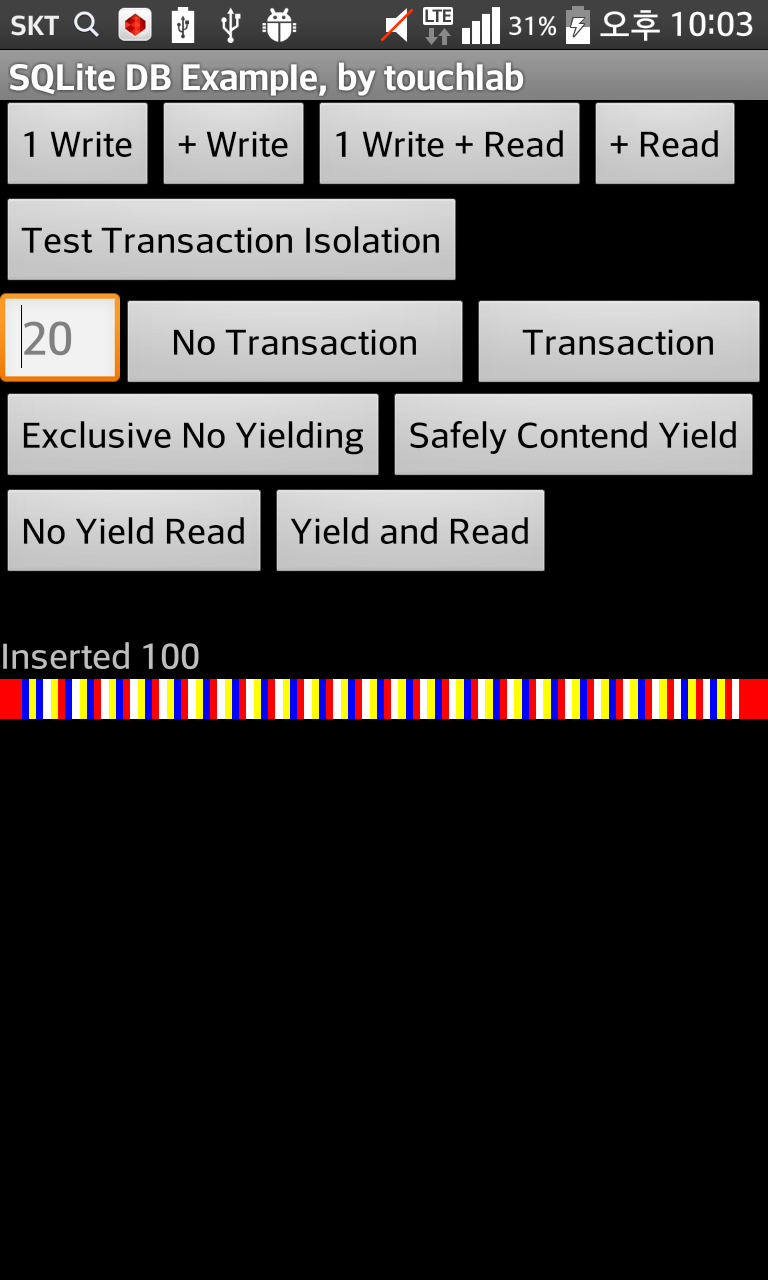
\includegraphics[scale=0.35]{device-sqlite}\\
File IO 성능이 좋지 않던 초기 안드로이드 단말에서는 Lock 문제가 쉽게 드러났지만, 최신 단말에서는 바로 눈에 띄지 않을 수도 있다.\footnote{버전이 높은 것이 항상 나은 것은 아니다. 4.0.4 버전의 특정 단말에서 Lock 에러가 많이 발생한 적도 있다.} 당장 보이지 않는다고 해서 사용자 단말에서도 문제가 없다고 생각하지 말자. QA 테스트에서는 거의 안 나타나던 Lock 에러가 배포 후에 사용자 단말에서는 다량으로 나타난 경우도 있었다.\\

Lock/트랜잭션 관련해서 테스트 가능한 샘플은 github에서 찾아볼 수 있다.\\
\url{https://github.com/touchlab/Android-Database-Locking-Collisions-Example}\\

이 샘플을 테스트한 결과를 얘기해보자.
\begin{enumerate}
\item 여러 스레드에서 1개의 SQLiteDatabase 인스턴스만 가지고 쓰기를 한다. 이때는 Lock 문제가 발생하지 않는다. 

\item 여러 스레드에서 각각 SQLiteDatabase 인스턴스를 가지고 쓰기를 한다. 이때는 Lock 문제가 발생한다. 여러 번 해봐도 문제가 잘 발생하지 않는다면 소스 상에서 스레드 개수를 늘려보자. 계속 늘려가보면 반드시 Lock 문제가 발생한다.

\item 1개의 스레드에서 1개의 SQLiteDatabase 인스턴스를 가지고 계속 쓰기를 하고, 여러 스레드에서 각각 SQLiteDatabase 인스턴스를 가지고서 읽기만 한다면 Lock 문제가 발생한다.

\item 여러 스레드에서 각각 SQLiteDatabase 인스턴스를 가지고서 읽기만 하면 Lock 문제가 발생하지 않는다.

\item 1개의 SQLiteDatabase 인스턴스를 가지고 쓰기 트랜잭션과 읽기를 동시에 실행한다. Lock 문제가 발생하지 않는다.

\item 1개의 SQLiteDatabase 인스턴스를 가지고 쓰기를 하는데 트랜잭션을 쓰지 않는 경우와 쓰는 경우를 비교할 수 있다. 트랜잭션을 쓰는 경우에 시간이 크게 줄어드는 것을 볼 수 있다.

\end{enumerate}

1$\sim$5번의 테스트에서 중요한 것은  SQLiteDatabase 인스턴스를 하나만 가지고 여러 스레드에서 명령을 실행해도 Lock 문제가 발생하지 않는다는 것이다. 이것은 SQLite의 default threading mode가 serialized이기 때문이다. 즉 명령어들은 순차적으로 실행되는 것이다.\footnote{\url{http://stackoverflow.com/questions/11167834/what-is-the-default-threading-mode-of-sqlite-in-android}}\\

threading mode 관련한 내용은 아래 url을 참고하자.\\
\url{http://www.sqlite.org/threadsafe.html}\\

SQLiteDatabase 인스턴스를 1개만 가지고서 serialized mode로 동작한다면 속도가 느려지진 않을까? 결론적으로 그렇다.
쓰기와 읽기가 함께 있는 것이라면 serialized mode가 되어야만 Lock 문제가 없기 때문에 1개의 인스턴스를 사용해야 하지만, 읽기만 있다면 굳이 1개의 인스턴스를 고집할 필요가 없다.\\

\begin{comment}
\subsubsection{Yield 하기}

\item Exclusive No Yielding과 Safely Contend Yield: SQLiteDatabase에는 yieldContendedSafely라는 메서드가 있어서, 다른 스레드의 명령이 실행되도록 트랜잭션을 끝내는 방법이 있다. 이게 호출될 때까지 성공한 것으로 간주하고 다시 새로운 트랜잭션이 생겨난다. 실행시간이 너무 길다 싶으면 다른 쪽에 양보를 하는 것인데, 전체 실행 속도에는 큰 차이가 보이진 않고, 다른 스레드의 명령이 너무 늦게 실행되는 것을 방지하는 측면에서 사용 가능하다. 이 테스트는 모두 다 쓰기 스레드이다.

\item No Yield Read와 Yield and Read: 쓰기 스레드와 읽기 스레드가 함께 있다. 쓰기 시간이 길어질 때 읽기 쪽에 양보하는 방식이다.
위에서 나온 Yield가 쓰일 만한 곳도 알아보자. 앱이 설치되고 처음 실행될때, 앱에서 사용할 기본 데이터를 위해서\footnote{이를테면 캘린더앱에서는 각 나라의 휴일 정보 같은 것이다. 한 해 것만 가져오는 것이 아니고 1900년부터 100년이 넘는 것을 모두 가져올 수도 있다. 음력이 있는 동양권에서는 더 많은 데이터가 필요하기도 하다.} API를 통해 서버에서 데이터를 가져올 수 있다. 만일 이것이 백만 건이 넘는 데이터라고 하면 JSON  데이터라고 해도 가져오는 데는 큰 부하까지는 걸리지 않을 것이다.\\
이것을 DB에 넣으려고 하면 당연히 Transaction으로 감싸야 한다.
그런데 앱은 처음 화면이 잘 뜨는 것도 중요하다. 
캘린더앱의 경우라면 처음 화면이 뜨고 일정을 조회하려고 DB 쿼리를 실행할 것이다. 그런데 앞에서 백만 건의 넘는 것을 Insert 하느라고 DB를 잡고 있다면, DB 쿼리를 실행할 수 없고 따라서 초기 실행 시간이 체감상 많이 느려질 수 있다.\\ 
그럼 10,000개마다 끊어서 Transaction을 매번 실행할 것인가 하면 그럴 필요가 없다. 바로 SQLiteDatabase.yieldContendedSafely를 10,000개마다 실행해주면 된다.
% 소스 있는 게 좋을 듯 하다. 정말 양보가 되는가?
\end{comment}

% 여기서 WAL을 넣어야 할 듯 하다.
% http://www.sqlite.org/wal.html
% http://sqlite.org/atomiccommit.html

%http://www.sqlite.org/datatype3.html

% http://beets.radbox.org/blog/sqlite-nightmare.html

%http://stackoverflow.com/questions/1005206/does-sqlite-lock-the-database-file-on-reads


%http://gywn.net/2013/08/let-me-intorduce-sqlite/

%http://www.sqlite.org/lockingv3.html
    
\begin{comment}
인덱스 문제가 있거나 테이블 조인 구조가 복잡하다면 쿼리 튜닝이 필요할 수 있다. EXPLAIN PLAN을 쓰는 방법이나 튜닝에 대한 기본 내용들은 인터넷에 많이 찾아 볼 수 있다.\\

09-05 18:47:27.335: E/Database(13396): close() was never explicitly called on database '/data/data/com.nhn.android.alarmclock/databases/alarms.db' 
09-05 18:47:27.335: E/Database(13396): android.database.sqlite.DatabaseObjectNotClosedException: Application did not close the cursor or database object that was opened here
09-05 18:47:27.335: E/Database(13396): 	at android.database.sqlite.SQLiteDatabase.<init>(SQLiteDatabase.java:1847)
09-05 18:47:27.335: E/Database(13396): 	at android.database.sqlite.SQLiteDatabase.openDatabase(SQLiteDatabase.java:820)
09-05 18:47:27.335: E/Database(13396): 	at android.database.sqlite.SQLiteDatabase.openOrCreateDatabase(SQLiteDatabase.java:854)
09-05 18:47:27.335: E/Database(13396): 	at android.database.sqlite.SQLiteDatabase.openOrCreateDatabase(SQLiteDatabase.java:847)
09-05 18:47:27.335: E/Database(13396): 	at android.app.ContextImpl.openOrCreateDatabase(ContextImpl.java:640)
09-05 18:47:27.335: E/Database(13396): 	at android.content.ContextWrapper.openOrCreateDatabase(ContextWrapper.java:203)
09-05 18:47:27.335: E/Database(13396): 	at android.database.sqlite.SQLiteOpenHelper.getWritableDatabase(SQLiteOpenHelper.java:118)
\end{comment}

\subsection{SQLiteOpenHelper}
SQLiteDatabase는 SQLite에 접근하는 클래스로, SQL 명령어를 실행하고 DB를 관리하는 메서드를 가지고 있다. SQLite를 사용하기 위해서는 꼭 거쳐야 하는 클래스이지만 실제 앱에서는 SQLiteDatabase를 직접 생성해서 사용하는 경우는 드물다.\footnote{/data/data/[패키지명]/databases가 아닌 다른 위치에 DB를 생성하거나 다른 앱(물론 앱의 공간이 아닌 public한 공간)의 DB를 읽고자 할 때는 SQLiteDatabase를 직접 사용해야 한다.}
바로 Helper 클래스인 SQLiteOpenHelper를 상속해서 사용하는데, SQLiteOpenHelper에서 Database 생성이나 Database 버전 관리를 알아서 해준다.\\

일반적으로 앱은 업데이트됨에 따라, DB에 테이블이 추가되거나 칼럼이 변경되고 앱에 필요한 기본 데이터가 추가되기도 한다. 
그래서 버전 관리는 필수적인데, SQLiteDatabase를 가지고 직접 하지 말고 반드시 SQLiteOpenHelper를 이용하도록 하자.
SQLiteOpenHelper는 추상 클래스이면서 일종의 Template Method 패턴을 만들어 놓은 것으로, 이 클래스를 상속해서 onCreate()와 onUpgrade() 메서드를 구현한 Database Helper를 작성하면 된다.\footnote{허니콤에서 onDowngrade() 메서드도 포함되었지만 이것은 추상 메서드는 아니어서 구현이 필수는 아니다.}\\

아래 코드는 ApiDemos에 있는 Database Helper를 조금 수정한 것이다.
\begin{lstlisting}[frame=single] 
public class DatabaseHelper extends SQLiteOpenHelper {

	private static final String DATABASE_NAME = "loader_throttle.db";
	private static final int DATABASE_VERSION = 2;

	DatabaseHelper(Context context) {
		super(context, DATABASE_NAME, null, DATABASE_VERSION); // (1)
	}

	@Override
	public void onCreate(SQLiteDatabase db) {
		db.execSQL("CREATE TABLE " + MainTable.TABLE_NAME + " ("
				+ MainTable._ID + " INTEGER PRIMARY KEY,"
				+ MainTable.COLUMN_NAME_DATA + " TEXT" + ");");
		...
	}

	@Override
	public void onUpgrade(SQLiteDatabase db, int oldVersion, int newVersion) {
		for (int i = oldVersion + 1; i <= newVersion; i++) { // (2)
			 processUpgrade(db, i);
		}
	}
}
\end{lstlisting}
여기서 살펴볼 게 몇 가지 있다.
\begin{itemize}
\item 7라인(1)의 생성자에 DATABASE\_NAME이 들어가는 것이 바로 DB 파일명이다.
그럼 DB를 여러 개 쓴다면 Database Helper도 여러 개 필요하다는 말일까? 그렇다. 한 앱에서 필요에 의해서 여러 DB를 사용할 수도 있고, 이때 기본적으로 Database Helper가 각각 필요하다.
가능하면 DB를 하나로 사용하는 것이 좋지만, 상황상 어쩔 수 없는 케이스도 있고 DB Lock 문제를 효과적으로 대응하기 위해서 DB를 분리할 수도 있다(읽기 전용 데이터를 위한 DB, 읽기+쓰기 용도 DB).\\

테이블이 동일하고 데이터 구조가 다른 게 없다면 그때는 어떡할까? 이를테면 로그인 기반의 앱이라면, 공통으로 사용하는 데이터를 위한 공통 DB가 있고 각 사용자별 DB가 있을 수 있다. 각 사용자별 DB는 당연히 동일한 테이블 구조를 갖고 있다. 이때는 DB 파일명을 상수를 만들지 않고 동적으로 전달하면 된다.
\begin{lstlisting}[frame=single] 
    DatabaseHelper(Context context) {
        super(context, getAuth().getLoginId() + ".db", null, DATABASE_VERSION);
    }
\end{lstlisting}

\item 생성자의 세 번째 파라미터는 거의 null을 넣는다. 
쿼리 결과로 Cursor 구현체인 SQLiteCursor를 쓰지 않는다면, Cursor 구현을 생성하는 Factory인 
SQLiteDatabase.CursorFactory를 새로 만들어서 파라미터에 전달할 수 있지만 필요한 경우가 사실상 없다.
%쿼리 결과로 SQLiteCursor를 쓰지 않는 경우라면, Cursor를 생성하는 SQLiteDatabase.CursorFactory를 새로 만들어서 넣는 게 가능하지만, 필요한 경우가 사실상 없다.

\item DB 생성은 어느 시점에 될까? SQLiteOpenHelper 생성자에서 하는 것으로 생각할 수 있지만 그렇지 않다.
실제로 DB 열기/생성(openOrCreate)은 SQLiteOpenHelper의 getReadableDatabase()나 getWritableDatabase() 메서드를 호출할 때이다.
더 정확하게 얘기하면 SQLiteOpenHelper에는 SQLiteDatabase 인스턴스를 1개 가지고 있는데 이 인스턴스가 앞에 이미 생성되었으면 그것을 사용하고, 그렇지 않은 경우에 생성하고서 onCreate()나 onUpgrade() 메서드가 실행된다.

\item DB 테이블 변경 시에는 Database Helper 생성자에 새로운 버전을 전달하고, 
SQLiteOpenHelper의 onUpgrade(SQLiteDtabase db, int oldVersion, int newVersion) 메서드에 변경 내용을 적용하면 된다. 이때 일반 패턴은 20라인(2)과 같이 for 문을 사용해서 oldVersion과 newVersion 범위 사이에 DB 버전에 했던 작업들을 처리하는 것이다.

\item onCreate() 메서드에는 최신 DB 스키마와 데이터를 반영해야 한다. 
onCreate() 메서드는 앱이 처음 DB를 생성할 때 호출된다. DB 버전이 1, 2, 3, 4 이렇게 바뀌면서 스키마와 데이터가 변경되었다고 하자. 버전이 1일 때 앱이 DB를 생성한다면 onCreate() 메서드가 호출되고, 중간에 앱을 업데이트하지 않다가 최신 버전으로 업데이트했다면 onUpgrade() 메서드가 호출된다.
그럼 버전이 4일때 처음 앱을 설치한다면 어떨까? 바로 onCreate() 메서드만 호출되고 onUpgrade() 메서드는 호출되지 않는다. 
개발하다 보면 onCreate()와 onUpgrade()가 순차적으로 호출되는 것으로 가끔 착각하게 되어서 언급하였다. onCreate()와 onUpgrade()는 둘 중에 하나만 호출된다.

\item DB 버전 업그레이드가 필요할 때 빠뜨려서는 안 된다. 예를 들어, 테이블 설계에 문제 있는 버전이 배포되었다고 하자.
마음 같아서는 다시 작성해서 동일한 버전으로 하면 코드도 깔끔할 것 같은데, 기존에 이 버전을 사용중인 단말은 DB 버전이 동일하므로 onUpgrade()는 실행되지 않고 변경된 테이블을 사용할 수 없다.
버전을 올리고서 onUpgrade()에서 테이블 구조를 변경하는 코드가 들어가는 게 정상적인 방법이다.

\item onCreate()와 onUpgrade() 메서드에서 하는 작업은 테이블 생성/수정 뿐 아니라 많은 기본 데이터 INSERT 등도 필요하다. 예를 들어, INSERT는 건당 시간이 얼마 안 걸리지만 1,000건, 10,000건이 된다면 속도가 대폭 떨어질 것을 예상할 수 있다.
그래서 트랜잭션을 쓰려고 하는데 SQLiteOpenHelper에는 이미 onCreate()와 onUpgrade() 메서드를 트랜잭션으로 감쌌기 때문에 또 다시 트랜잭션을 고려할 필요가 없다.\footnote{SQLiteOpenHelper가 Template Method로서 의미 있는 부분이다.}

\item DATABASE\_NAME 위치에 null을 넣으면 파일 DB가 아닌 메모리 DB가 된다. 파일 DB라도 속도가 느리진 않지만 메모리 DB는 그보다 훨씬 속도가 빠르다. DB가 닫히면 함께 사라져버리는 휘발성 DB이므로 일종의 캐시 용도로 사용하는 것이 좋다.
코드 상에서 캐시 자료구조를 만들어도 되는데, 굳이 메모리 DB를 쓰면 좋은 케이스는 무엇일까? 바로 그 안에서 쿼리를 실행할 수 있다는 점이다.
예를 들어, 여러 칼럼이 있고 각 칼럼별로 정렬을 바꾸어주는 기능이 있다면, 정렬할 때마다 File IO를 하는 것보다는 메모리 DB에 담아놓고서 쿼리로 정렬하면 결과가 훨씬 빨라진다. 
파일 DB에서 원시(raw) 데이터를 가져와서 조합해서 생성한 결과 목록을 메모리 DB에 저장해서 사용하는 것도 고려해 볼 수 있다.\\

당연한 얘기지만 메모리 DB에서는 DB 버전 업그레이드가 의미가 없으므로 version은 신경쓸 필요가 없다. 1로 놓고 다시는 변경하지 말자.

\item Database Helper는 앱 전체에 걸쳐 단일 인스턴스를 가지고 있어야 DB Lock 문제에서 자유롭다. 
그래서 일반적으로 아래와 같이 싱글톤 패턴을 만들어서 사용한다. 싱글톤 패턴에 대해서 11장에서 다시 설명하기로 한다.
\begin{lstlisting}[frame=single] 
public static DatabaseHelper extends SQLiteOpenHelper  {
   private static DatabaseHelper instance;
 
  public static synchronized DatabaseHelper getInstance(Context context) {
     if (instance == null) {
        instance = new DatabaseHelper(context.getApplicationContext()); // (1)
     }
    return instance;
   }
 
   private DatabaseHelper(Context context) {
       ...
   }
}
\end{lstlisting}
6라인(1)에서 context가 아닌 context.getApplicationContext()를 전달한 것을 주목하자.
생성자가 private으로 감추어져 있으므로 사용하는 쪽에서는 getInstance()로 가져와서 사용한다.
\begin{lstlisting}[frame=single] 
DatabaseHelper dbHelper = DatabaseHelper.getInstance(context);
\end{lstlisting}

\item close() 메서드는 실제 호출할 일이 거의 없다.
SQLiteOpenHelper의 close()는 SQLiteDatabase 인스턴스의 close()를 호출하고, SQLiteDatabase 인스턴스를 null로 만든다. 
매번 close()를 호출하지 않고서 SQLiteDatabase 인스턴스를 계속 재사용해도 문제가 없고, 또 다른 이유는 close() 실행 시점 때문에 문제가 발생할 수 있다는 것이다.\\

A 스레드에서 getWritableDatabase()를 실행하고서 쿼리를 실행하려 한다고 하자. B 스레드에서는 뭔가 작업을 하고 close()를 실행한다. 시점에 따라서 A 스레드에서 getWritableDatabase() 이후에 B 스레드에서 close()가 실행되고, 이것을 가지고 A 스레드에서 쿼리한다면  NullPointerException이 발생하게 된다. 
%  에러 메시지 보여주자
\item onConfigure(SQLiteDatabase db) 메서드와 onOpen(SQLiteDatabase db) 메서드가 있다. onConfigure() 메서드는 SQLiteDatabase 생성/열기 이후, onCreate()와 onUpgrade() 메서드 전에 실행되는 것으로 write-ahead logging이나 foreign key support 같은 기능을 활성화하는 작업 등을 할 수 있다. onOpen() 메서드는 onCreate()와 onUpgrade() 이후에 database connection 설정을 변경할 때 사용한다.

\end{itemize}

\section{ContentProvider}
ContentProvider는 여러 앱 간에 데이터를 공유할 필요가 있을 때 사용한다. 데이터 소스는 굳이 DB일 필요는 없다. 
파일이든 네트워크를 통해서 구하는 값이든 다 데이터 소스로 가능하다. 다만 API가 DB를 데이터 소스로 사용하는 것에 더 맞게 디자인되어 있다.\\

ContentProvider 접근은 ContentResolver를 통해서만 가능하다. 그리고 Context의 getContentResolver() 메서드를 통해서만 ContextResolver를 구할 수 있다.  
% 그림 필요
ContextResolver는 일종의 Proxy인데, 해당하는 Uri의 ContentProvider를 찾는 역할을 한다.
% 퍼미션 체크는 ContentProvider에서 한다.
ContentResolver는 추상 클래스이고 실제 사용하는 클래스는 ContextImpl의 내부 클래스인 ApplicationContentResolver이다.

\subsection{ContentProvider 적용}
개발자 가이드에 의하면 로컬 프로세스에서만 사용하려면 ContentProvider를 사용하지 않는 것이 권장된다. 
ContentResolver를 거치는 것보다 직접 DB를 접근하는 것이 속도가 훨씬 빠르다.\\

한 앱에서도 ContentProvider를 쓰면 유용한 경우를 들어보자(이 때문에 어떤 문서에서는 가능하면 DB 관련 코드는 ContentProvider를 쓰라고 하기도 한다).
\begin{itemize}
\item 메서드 시그너처를 따라야 하므로 API 일관성을 유지할 수 있다.
\item CursorLoader, AsyncQueryHandler와 같은 유용한 클래스들이 ContentProvider의 Uri가 전달되어야만 동작한다.
\item 한 앱에서도 프로세스가 분리될 수 있다. 이를테면 Service가 메모리 사용이 많아서 프로세스를 분리하고 각 프로세스에서 Database Helper를 사용한다면, 싱글톤이 유지되지 않아서 Lock 문제가 언제든 발생할 수 있다.
이때 앱 프로세스에 ContentProvider를 두고, 이 ContentProvider를 Service 프로세스에서 ContentResolver를 통해서 접근하면 유일한 Database Helper를 유지할 수 있다. %이미지 추가?
\end {itemize}

그럼 로컬 프로세스에서 ContentProvider를 쓰는 단점은 무엇일까?
\begin{itemize}
\item 직접 DB에 접근하는 것에 비해서 속도가 조금 느리다.
\item groupBy, having, limit 같은 파라미터를 ContentResolver의 메서드에 전달할 수 없다. 
필요한 경우 Uri나 쿼리 파라미터에 억지로 끼워넣어서 전달해야 한다. 
\item ContentResolver를 통하므로 별도의 public 메서드를 만들어도 접근할 수 없다.
\end {itemize}

가이드가 혼재되어 있는데 결론을 내려보자.
로컬 프로세스에서는 ContentProvider를 쓰지 않는 것을 먼저 고려하자. ContentProvider를 사용하는 장점이 꼭 필요하다면, 그때 ContentProvider를 쓰기로 하자.
다만 직접 DB에 접근하는 코드에서도 메서드 시그너처를 ContentProvider와 유사하게 만들면, 이후에 변경이 수월할 수 있다.
프로세스가 분리되거나 다른 앱에서 DB 접근이 필요하다면, 필요한 부분만 ContentProvider로 접근해서 DB Access(내부용) + ContentProvider(외부용)으로 하는 것도 가능한 방법이다.\\

%https://thenewcircle.com/s/post/1375/android_content_provider_tutorial

코드 \ref{src:provider}은 안드로이드 샘플 프로젝트인 NotePad에서 ContentProvider를 만든 예이다. 
ContentProvider는 다른 컴포넌트와는 달리 만드는 방법이 정형화되어 있다. 
ContentResolver를 통해서만 접근하기 때문에 별도의 public 메서드는 의미가 없다.

\begin{lstlisting}[frame=single, caption=ContentProvider 예, label=src:provider] 
public class NotePadProvider extends ContentProvider {
	private static final String TAG = "NotePadProvider";

	private static final String DATABASE_NAME = "note_pad.db";
	private static final int DATABASE_VERSION = 2;

	...

	private static final UriMatcher sUriMatcher;

	private DatabaseHelper mOpenHelper;

	static {
		sUriMatcher = new UriMatcher(UriMatcher.NO_MATCH);
		sUriMatcher.addURI(NotePad.AUTHORITY, "notes", NOTES);
		sUriMatcher.addURI(NotePad.AUTHORITY, "notes/#", NOTE_ID);
		...
	}

	static class DatabaseHelper extends SQLiteOpenHelper {

		DatabaseHelper(Context context) {
			super(context, DATABASE_NAME, null, DATABASE_VERSION);
		}

		@Override
		public void onCreate(SQLiteDatabase db) {
			db.execSQL("CREATE TABLE " + NotePad.Notes.TABLE_NAME + " ("
					+ NotePad.Notes._ID + " INTEGER PRIMARY KEY,"
					+ NotePad.Notes.COLUMN_NAME_TITLE + " TEXT,"
					+ NotePad.Notes.COLUMN_NAME_NOTE + " TEXT,"
					+ NotePad.Notes.COLUMN_NAME_CREATE_DATE + " INTEGER,"
					+ NotePad.Notes.COLUMN_NAME_MODIFICATION_DATE + " INTEGER"
					+ ");");
		}

		@Override
		public void onUpgrade(SQLiteDatabase db, int oldVersion, int newVersion) {
			...
		}
	}

	@Override
	public boolean onCreate() {
		mOpenHelper = new DatabaseHelper(getContext()); // (1)
		return true;
	}

	@Override
	public Cursor query(Uri uri, String[] projection, String selection,
			String[] selectionArgs, String sortOrder) {
		...
		SQLiteDatabase db = mOpenHelper.getReadableDatabase();

		Cursor c = qb.query(db, // The database to query
				projection, // The columns to return from the query
				selection, // The columns for the where clause
				selectionArgs, // The values for the where clause
				null, // don't group the rows
				null, // don't filter by row groups
				orderBy // The sort order
				);

		c.setNotificationUri(getContext().getContentResolver(), uri);
		return c;
	}

	@Override
	public String getType(Uri uri) {
		switch (sUriMatcher.match(uri)) {
		case NOTES:
			return NotePad.Notes.CONTENT_TYPE;
		case NOTE_ID:
			return NotePad.Notes.CONTENT_ITEM_TYPE;
		default:
			throw new IllegalArgumentException("Unknown URI " + uri);
		}
	}

	@Override
	public Uri insert(Uri uri, ContentValues initialValues) {
		...
		SQLiteDatabase db = mOpenHelper.getWritableDatabase();
		long rowId = db.insert(NotePad.Notes.TABLE_NAME,
				NotePad.Notes.COLUMN_NAME_NOTE, 
				values 
				);

		if (rowId > 0) {
			Uri noteUri = ContentUris.withAppendedId(
					NotePad.Notes.CONTENT_ID_URI_BASE, rowId);
			getContext().getContentResolver().notifyChange(noteUri, null);
			return noteUri;
		}
		throw new SQLException("Failed to insert row into " + uri);
	}

	@Override
	public int delete(Uri uri, String where, String[] whereArgs) {
		SQLiteDatabase db = mOpenHelper.getWritableDatabase();
		...
		count = db.delete(NotePad.Notes.TABLE_NAME, // The database table name
					finalWhere, // The final WHERE clause
					whereArgs // The incoming where clause values.
					);

		..
		getContext().getContentResolver().notifyChange(uri, null);
		return count;
	}

	@Override
	public int update(Uri uri, ContentValues values, String where,
			String[] whereArgs) {
		SQLiteDatabase db = mOpenHelper.getWritableDatabase();
		...
		count = db.update(NotePad.Notes.TABLE_NAME, 
					values, 
					where, 
					whereArgs 
					);
		...
		getContext().getContentResolver().notifyChange(uri, null);
		return count;
	}

}
\end{lstlisting}
\begin{itemize}
\item ContentProvider를 사용하면 멀티 스레드 환경에서 Lock 문제가 없이 잘 동작하기 때문에 ContentProvider에서 Lock을 제어한다고 오해하는 경우가 있다. 
Lock 문제가 발생하지 않는 것은 ContentProvider를 써서 그런 것이 아니라 ContentProvider를 만드는 일반적인 패턴으로 인한 것이다.
45라인(1)을 보면 onCreate() 메서드에서 Database Helper를 하나 생성해놓고 이것을 사용하고 있다.
onCreate()는 처음 ContentProvider를 사용할 때 단 한번만 실행되고, ContentProvider는 단말에서 오직 하나만 존재하기 때문에 Database Helper도 오직 하나뿐이다. 따라서 내부적으로 명령어가 serialization되면서 Lock 문제가 없는 것이다.

\item ContentProvider의 onCreate() 메서드는 Application의 onCreate() 메서드 이전에 실행된다.\footnote{ActivityThread의 handleBindApplication() 메서드를 분석해보자.}
따라서 Application의 onCreate() 메서드가 먼저 실행된다고 가정하면 안된다.
복잡한 앱에서는 Application의 onCreate() 메서드에서 앱 전체적으로 사용하는 인스턴스를 미리 생성하는 역할을 하기도 한다. ContentProvider에서도 Application에서 생성한 것을 쓰고 싶지만 순서를 주의하도록 하자.
ContentProvider의 onCreate()는 메인 스레드에서 실행하고 다른 메서드는 일반적으로 별도 스레드에서 실행하므로(로컬에서도 ContentProvider는 스레드에서 호출하도록 권장되고, Binder를 통한 외부 앱의 접근은 Binder 스레드를 거쳐 실행), ContentProvider의 메서드 간에는 스레드 안정성에 주의하도록 하자. 멤버 변수를 함부로 쓰면 안된다는 얘기이다.

\item insert/update/delete 메서드에서 DB 명령 실행 후에 getContext().getContentResolver().notifyChange\-(uri, null)를 호출한다. ContentResolver에는 registerContentObserver() 메서드가 있어서 데이터가 변경되면 알 수 있도록 ContentObserver를 등록하는데, 이 ContentObserver에 알림을 주기 위한 것이다. 
ContentObserver에는 어떤 데이터가 변경되었는지 알리지는 않고 변경되었는지 여부만 전달한다. 
그러면 무슨 쓸모가 있는가 의문이 생기는데,
query() 메서드에서 리턴 결과인 Cursor에는 requery()라는 메서드가 있어서 새로 조회할 수 있다. 특히 CursorAdaper는 내부에 ContentObserver가 등록되어 있어서 notifyChange()를 받으면 requery()를 실행한다.

\end{itemize}
% ContentProvider call 메서드도 있다.(이것이 안드로이드다 참고)

\subsection{배치 execute}
% http://surprisen.egloos.com/2504139
ContentProvider에서는 여러 명령어를 한꺼번에 실행할 수 있는 applyBatch() 메서드를  제공한다. 
applyBatch() 메서드를 보면 속도 향상을 위해서 트랜잭션을 쓰는 것으로 혼동할 수도 있지만, 실제로 하는 일은 ContentProviderOperation 목록을 한꺼번에 전송해놓고 순차적으로 수행하는 것에 지나지 않는다. 
\begin{lstlisting}[frame=single] 
ArrayList<ContentProviderOperation> operations 
	= new ArrayList<ContentProviderOperation>();
operations.add(ContentProviderOperation.newInsert(NotePad.CONTENT_URI) // (1)
	.withValue(NotePad.Notes.COLUMN_NAME_TITLE, "Lunch")
	.withValue(NotePad.Notes.COLUMN_NAME_NOTE, "Kimchi")
	.withValue(NotePad.COLUMN_NAME_CREATE_DATE, 
		Long.valueOf(System.currentTimeMillis()))
	.build());
operations.add(ContentProviderOperation.newUpdate(NotePad.CONTENT_URI) // (2)
	.withSelection(NotePad.Notes._ID + "=?", new String[] {3})
	.withValue(NotePad.Notes.COLUMN_NAME_TITLE, "Lunch2")
	.withValue(NotePad.Notes.COLUMN_NAME_NOTE, "Kimchi2")
	.withValue(NotePad.Notes.COLUMN_NAME_MODIFICATION_DATE, 
		Long.valueOf(System.currentTimeMillis()))
	.build());
operations.add(ContentProviderOperation.newDelete(Memos.CONTENT_URI) // (3)
	.withSelection(NotePad.Notes._ID + "=?", new String[] {5})
	.build());

mContext.getContentResolver().applyBatch(NotePad.AUTHORITY, operations); // (4)
\end{lstlisting}
\begin{itemize}
\item 3라인(1), 9라인(2), 16라인(3)에서 ContentProviderOperation(Insert/Update/Delete용)을 ArrayList에 추가한다. 
newInsert/newUpdate/newDelete 같은 메서드는 Builder 패턴을 사용해서 ContentProviderOperation 인스턴스를 만들어 낸다.
\item 20라인(4)에서 applyBatch() 메소드를 통해 ArrayList에 쌓아둔 작업들을 한꺼번에 보낸다.
\end{itemize}

다른 프로세스에서 실행한다면 Binder를 거쳐야 하는데, 하나씩 명령어를 주고받는 것보다 한꺼번에 보내는 것으로 속도 향상은 있지만 트랜잭션을 쓰는 것처럼 속도 향상이 큰 것은 아니다.
트랜잭션을 써서 속도를 향상시키고 싶다면,
ContentProvider에서 applyBatch(ArrayList$<$ContentProviderOperation$>$ operations) 메서드를 오버라이드하는 방법이 있다.
\begin{lstlisting}[frame=single] 
@Override
public ContentProviderResult[] applyBatch(
		ArrayList<ContentProviderOperation> operations) {
	SQLiteDatabase db = mOpenHelper.getWritableDatabase();
	db.beginTransaction();
	try {
     	ContentProviderResult[] result = super.applyBatch(operations);
     	db.setTransactionSuccessful();
     	return result;
   	} finally {
     	db.endTransaction();
   	}
}
\end{lstlisting}
트랜잭션으로 감싸는 코드를 applyBatch() 메서드에 적용하였다.

\begin{comment}
\begin{lstlisting}[frame=single] 
07-08 10:13:30.923: E/SQLiteOpenHelper(25079): android.database.sqlite.SQLiteDatabaseLockedException: database is locked (code 5): , while compiling: PRAGMA journal_mode
07-08 10:13:30.923: E/SQLiteOpenHelper(25079): 	at android.database.sqlite.SQLiteConnection.nativePrepareStatement(Native Method)
\end{lstlisting}

SQLiteQueryBuilder.buildQueryString 이것으로 쿼리문 결과 볼 수 있다.

bulk insert update
http://www.mysamplecode.com/2011/10/android-sqlite-bulk-insert-update.html

I/O 발생으로 가능하면, AsyncTask 나 별도 Thread에서 실행하는 것을 권장한다.
API 11에서부터 CursorLoader를 사용할 수 있는데, AsyncTask를 사용해서, Content Provider를 통해서 값을 가져온다.

LIKE 구문은 신경을 쓰자..
http://www.mail-archive.com/sqlite-users@sqlite.org/msg14482.html

필요한 경우 index를 생성한다.


% http://androcat.egloos.com/1778615
% http://developer.android.com/training/notepad/notepad-ex3.html
% http://stackoverflow.com/questions/4940308/im-getting-a-database-object-not-closed-exception-in-sqlite-android-but-im
 

%http://www.enterra-inc.com/techzone/handling_sql_issues/

remote에서 contentProvider를 호출할 경우 CursorWindow를 복사해버린다. multiprocess는 확인해봐야 한다.


Conent Provider를 사용하지 않을 때에는 칼럼명을 굳이 상수화 하지 않도록 한다.

%http://stackoverflow.com/questions/2647542/android-threading-and-database-locking
%http://www.androiddesignpatterns.com/2012/05/correctly-managing-your-sqlite-database.html
%http://charlie0301.blogspot.kr/2013/07/sqlite-and-android-sqlite.html

content prefix는 content provider에 의해 데이타가 제공된다는 의미이다.

content://com.example.transportationprovider/trains

ContentProvider의 insert 메서드는 리턴이 Uri로 받은 값을 가지고 입력한 id를 얻을 수 있다.
\begin{verbatim}
long rowId = database.insert(values);

		if (rowId > 0) {

			Uri memoUri = ContentUris.withAppendedId(CONTENT_URI, rowId);

      getContext().getContentResolver().notifyChange(memoUri, null);

			return memoUri;

		}

=>

			String id = uri.getPathSegments().get(1);
\end{verbatim}



액티비티에서는  managedQuery  메서드를 바로 사용하면 된다.
insert, update, delete는 getContentResolver() 하고서 메서드를 호출한다.
\end{comment}

\section{SQLite/ContentProvider 관련 팁}
\subsection{쿼리 실행 확인}
일반적으로 쿼리 속도를 체크하기 위해서 코드 상에 쿼리 실행 전후 시간 차이를 로그로 남겨서 확인한다.
이 방식도 지속적으로 확인이 필요할 때는 유용하지만, 그 시기가 지나면 불필요한 로깅 코드가 남게 된다.
단순하게 실행 속도를 체크하는 방법을 보자.\\

adb shell에서 dumpsys dbinfo를 하면 DB 별로 최근 쿼리 실행 속도와 바인드된 파라미터들(bindArgs)을 확인할 수 있다(단말에서는 보안상 bindArgs가 잘 나오지 않는다).
가장 최근 것부터 나오므로 순서상 밑의 것부터 보아야 한다(쿼리를 prepare하고 execute하는 것을 볼 수 있다).

\begin{lstlisting}[frame=single] 
** Database info for pid 1008 [system] **

Connection pool for /data/data/com.android.providers.settings/databases/settings.db:
  Open: true
  Max connections: 4
  Available primary connection:
    Connection #0:
      isPrimaryConnection: true
      onlyAllowReadOnlyOperations: false
      Most recently executed operations:
        0: [2014-09-30 10:40:04.548] executeForLastInsertedRowId took 5ms 
        	- succeeded, sql="INSERT INTO system(value,name) VALUES (?,?)", 
			bindArgs=["1", "volume_ring_last_audible_speaker"]
        1: [2014-09-30 10:40:04.548] prepare took 0ms - succeeded, 
        	sql="INSERT INTO system(value,name) VALUES (?,?)"
	...
  Available non-primary connections:
    Connection #1:
      isPrimaryConnection: false
      onlyAllowReadOnlyOperations: true
      Most recently executed operations:
        0: [2014-09-30 11:32:32.135] executeForCursorWindow took 0ms 
        	- succeeded, sql="SELECT _id, name, value FROM secure"
        1: [2014-09-30 11:32:32.135] prepare took 0ms - succeeded, 
        	sql="SELECT _id, name, value FROM secure"
	...
  Acquired connections:
    <none>
  Connection waiters:
    <none>
\end{lstlisting}
dumpsys dbinfo 명령어도 모든 앱의 DB 히스토리를 모두 출력하기 때문에 내용이 많다. dbinfo에 쓸 수 있는 옵션은 pid가 있다. 
만일 com.suribada.myhome 패키지의 DB 쿼리 내용을 알고 싶다면 ps | grep com.suribada.myhome으로 pid를 알아낸 다음에 dumpsys dbinfo 1004 와 같이 실행하면 된다.\\

dumpsys dbinfo 명령어는 속도 체크 뿐 아니라 쿼리가 원하는 시점에 실행되는지 체크하는데도 쓰일 수 있다.
여러 스레드에서 쿼리를 실행한다면, 일상적으로 문제가 없다가도 특정한 조건에서 가장 필요로 하는 쿼리가 곧바로 실행되지 않을 수 있다.\\

예를 들어, 화면이 처음 실행될 때에 내부적으로 서버와 데이터 동기화가 실행되면서 화면에도 데이터를 조회해서 보여줘야 한다. 
동기화 중에는 트랜잭션 구간이 있는데 동기화할 데이터가 많고 이런 트랜잭션이 먼저 실행된다면, 조회 쿼리는 그 이후로 미뤄지고 만다. 
동기화할 데이터가 많은 상태까지 테스트하지 못해서, 이런 케이스는 개발 중에는 잘 모를 수도 있다.\\

관련해서 샘플을 만들어보자.
\begin{lstlisting}[frame=single] 
	private DictionaryOpenHelper dbHelper;

	@Override
	protected void onCreate(Bundle savedInstanceState) {
		super.onCreate(savedInstanceState);
		...
		dbHelper = DictionaryOpenHelper.getInstance(this); // (1)
	}

	public void onClickButton1(View view) {
		new Thread(new Runnable() { // (2)

			@Override
			public void run() {
				Log.d("suribada", "Thread1 start");
				SQLiteDatabase db = dbHelper.getReadableDatabase();
				Cursor cursor = db.query(WordTable.TABLE_NAME, 
					null, null, null, null, null, WordTable.COLUMN_KEYWORD); // (3)
				Log.d("suribada", "cursor.count=" + cursor.getCount());
				cursor.close();
			}

		}).start();
		
		new Thread(new Runnable() { // (4)

			@Override
			public void run() {
				Log.d("suribada", "Thread2 start");
				SQLiteDatabase db = dbHelper.getWritableDatabase();
				Random random = new Random();
				db.beginTransaction(); // (5)
				try {
					for (int i = 0; i < 10; i++) {
						int num = random.nextInt(1024);

						ContentValues values = new ContentValues();
						values.put(WordTable.COLUMN_KEYWORD, "apple" + num);
						values.put(WordTable.COLUMN_DEFINITION, 
							"a round fruit " + num);
						values.put(WordTable.COLUMN_PRONUNCIATION, "aepl " + num);
						values.put(WordTable.COLUMN_LAST_UPDATE_TIME,
							System.currentTimeMillis());
						db.insert(WordTable.TABLE_NAME, null, values);
						SystemClock.sleep(1000); // (6)
					}
					db.setTransactionSuccessful();
				} finally {
					db.endTransaction();  // (7)
				}
			}

		}).start();
	}
\end{lstlisting}	
\begin{itemize}
\item 7라인(1)에서 여러 스레드에서 공통으로 사용할 dbHelper 변수를 생성하였다. DB Lock 문제가 발생하지 않으려면 하나의 dbHelper를 사용해야 한다.
\item 11라인(2)과 25라인(4)에서 2개의 스레드를 시작한다.
11라인의 스레드는 단순 조회이다.
25라인의 스레드는 데이터를 10개 입력하는데 45라인(6)에서 1초간 sleep하기 때문에(시간이 걸리는 것을 시뮬레이션) 최소 실행 시간은 10초이다. 32라인(5)에서 트랜잭션을 시작하고 49라인(7)에서 트랜잭션을 종료한다.
\item 스케줄링에 의해서 첫 번째 스레드가 운 좋게 먼저 실행된다면 다행이지만, 두 번째 스레드의 32라인(5)에서 beginTransaction() 메서드가, 첫 번째 스레드의 17라인(3)에서 query() 메서드보다 먼저 실행된다면 어떤 일이 발생할까? 바로 명령어가 serialization되기 때문에 두 번째 스레드의 49라인(startTransaction $\sim$ endTransaction)까지 첫 번째 스레드의 18라인이 대기한다. 사용자 입장에서는 단순 조회라서 금방 되어야 하는데 10초 이상이 걸리는 것이다. 
\end{itemize}

이 상황은 앞서 얘기한 동기화를 하느라고 조회 쿼리가 늦어지는 것과 동일한 케이스이다. 
서버와 데이터를 동기화하는 앱에서 많이 쓰이는 패턴은 아래와 같다.
\begin{enumerate}
\item startService()를 실행하여 Service의 백그라운드 스레드에서 서버 데이터를 가져와 DB에 반영한다. 이때 속도 향상을 위해서 트랜잭션을 사용한다(시간이 얼마나 걸릴지 알 수 없다. 사용자 데이터는 천차만별이다).
\item 첫 화면은 AsyncTask를 이용해서 기존 DB의 데이터를 조회해서 UI에 반영한다. 
\item 동기화가 완료되면 DB에 다 반영되었으므로 Service에서 sendBroadcast()를 실행하고 화면에서는 AsyncTask로 변경된 결과를 다시 조회한다.
\end{enumerate}

1번 때문에 2번이 늦어지는 상황이 이해될 것이다. 원리를 모른다면 ``도대체 왜 그럴까?''하면서 해결할 수 없는 문제가 된다. 
필자의 경우에도 이 문제를 처음 겪었을 때 원인을 미처 생각하지 못했던 기억이 있다. 
그럼 이 문제는 어떻게 해결해야 할까? 바로 2번 작업이 최초 한번은 실행되고 난 다음에 startService()를 실행하는 것이다. 
단지 순서를 바꾸기만 하면 되는 것이다.\\

원하는 시점에 쿼리가 실행되지 않는 원인으로, 사용하는 라이브러리의 쿼리 문제 가능성도 생각할 수 있다. 이를테면 전체 공휴일 정보를 제공하는 라이브러리에서 DB로 정보를 제공할 수도 있다.\\

문제 상황이 발생했을 때 dumpsys를 통해 확인해보고, 실행 시점을 조정하거나 라이브러리를 재검토해보자.

\subsection{ContentProvider 예외 확인}
외부 프로세스에서 ContentProvider에 접근할 때 ContentProvider를 제공하는 쪽에서 문제가 발생하면, 예외 스택이 그대로 외부 프로세스에 전달되지 않는다.
아래처럼 NullPointerException이 발생했지만, 왜 발생했는지 더 이상 스택이 보이지 않는 걸 볼 수 있다.
\begin{lstlisting}[frame=single] 
Caused by: java.lang.NullPointerException 
	at android.os.Parcel.readException(Parcel.java:1471) 
at android.database.DatabaseUtils.readExceptionFromParcel(DatabaseUtils.java:185) 
at android.database.DatabaseUtils.readExceptionFromParcel(DatabaseUtils.java:137) 
at android.content.ContentProviderProxy.query(ContentProviderNative.java:413) 
at android.content.ContentResolver.query(ContentResolver.java:464) 
at android.content.ContentResolver.query(ContentResolver.java:407
...
\end{lstlisting}
DB가 데이터 소스인 경우는 별로 그럴 일이 없지만, 네트워크나 파일, 또는 로직을 통해 생성한 결과 등을 데이터 소스로 사용한다면 이런 예외 케이스는 원인을 확인해야 한다.\\

그럼 ContentProvider를 제공하는 쪽에서는 크래시가 발생하는가 하면 그렇지 않다. 바로 Exception을 잡아서 Binder로 전달하는 값에 숫자를 전달하고, DatabaseUtils 태그로 ERROR 레벨을 가지고 로그를 남긴다.\footnote{/frameworks/base/core/java/android/database/DatabaseUtils.java를 확인하자.}
ContentProvider에서는 DatabaseUtils 태그로 문제를 확인하도록 하자.
% 샘플 만들자.
% 그밖의 예외에 대해서는 어떻게 되지?


\chapter{BroadcastReceiver}
BroadcastReceiver는 Observer 패턴\footnote{\url{http://warmz.tistory.com/751}를 참고하자.}을 안드로이드에서 구현한 방식이다.
한 쪽에서 뭔가 특별한 이벤트가 발생했을때 다른 쪽에서도 해야 할 작업이 있다.
예를 들어, 안드로이드 책이 한 권 출판되어서(1) 출판사에서 연락하면(2), 각 온라인 서점에서는 데이터를 각각 입력해야만 한다(3). BroadcastReceiver 입장에서 보면 1번은 Intent 내용, 2번은 sendBroadcast() 메서드 호출, 3번은 onReceive() 메서드에 대응된다.\\

Observer 패턴에서는 일대다 관계에서 직접 호출하지 않고, 인터페이스를 통한 느슨한 결합을 통해 Observer를 register/unregister하는 방법을 제공한다.
이 방식은 BroadcastReceiver에서도 마찬가지이다. BroadcastReceiver는 바로 Observer이고, 이벤트는 sendBroadcast()에 전달되는 Intent이다(이벤트는 여러 곳에 퍼뜨리기 위한 방송용 이벤트라고 보면 된다). Context에는 registerReceiver()와 unregisterReceiver() 메서드가 있어서 여러 컴포넌트(Activity, Service, Application)에서 사용할 수 있다.

\section{BroadcastReceiver 구현}
BroacastReceiver에는 추상 메서드가 하나뿐이고 나머지 메서드는 사용할 일이 많지 않다.
\begin{verbatim}
	abstract void onReceive(Context context, Intent intent)
\end{verbatim}

BroadcastReceiver는 ContentProvider와 마찬가지로 ContextWrapper 하위 클래스가 아니다. 그러나 Context는 전달되므로 이것을 가지고 할 수 있는 게 있다.\footnote{onReceive() 메서드에 전달되는 Context는 Application의 Context이다.}
startService(), startActivity() 외에도 sendBroadcast()를 다시 호출할 수도 있다. 
이벤트가 발생하면 그 이벤트에 대응해서 화면을 보여주거나 백그라운드 작업이 필요한 경우가 많기 때문에, 실제로 실행하는 주된 일이 startService()나 startActivity()이다. \\

방송용 이벤트가 발생할 때 직접적으로 startService()나 startActivity()를 실행하는 방법은 없다. 이벤트는 바로 방송의 형태를 띄기 위해서 sendBroadcast()를 통해서 전달되고, 이때 화면을 띄우려면 BroadcastReceiver의 onReceive() 메서드에서 startActivity()를 실행하고, UI가 없는 내부 작업이 필요하다면 startService()를 실행한다.\\

Line이나 카카오톡 같은 메신저 앱의 경우를 보자. 누군가 내게 메시지를 보내면 Push Message를 BroadcastReceiver에서 받는다. 그 순간에 `띵동' 소리가 나고 화면에 `팟' 하면서 팝업에 대화 내용이 뜨는데, 이 팝업이 바로 onReceive() 메서드에서 startActivity()를 실행한 결과이다.\\

onReceive()에서 startService()와 startActivity()를 둘 다 실행하는 경우도 있다. 특정 이벤트가 발생할 때 배경 음악(화면이 닫혀도 배경 음악이 유지되어야 한다고 가정)이 깔리면서 화면이 떠야 한다면, 배경 음악이 깔리는 것은 startService()를 실행해야 하고 화면이 뜨는 것은 startActivity()를 실행해야 한다.\\

onReceive() 메서드는 메인 스레드에서 실행되므로 시간 제한도 있다.
10초(포그라운드)/1분(백그라운드: 기본)내에 onReceive() 메서드 실행이 끝나야 한다. 10초/1분이 넘으면 ANR이 발생한다.
메인 쓰레드에서 실행되므로 실제로는 1분/10초/5초도 아닌 훨씬 짧은 시간내에 처리가 완료되어야 한다. 그렇지 않으면 UI에서 버벅거림의 원인이 될 수 있다.\\

한 이벤트에 대해서 한 앱에 여러 BroadcastReceiver가 등록된 경우도 주의해야 한다.
본래 Broadcast는 여러 프로세스 간에 이벤트를 전달하기 위한 것이다. 각 프로세스라면 동시에 실행되는 데 문제가  없지만, 한 앱에서는 여러 개의 BroadcastReceiver가 있을 때 onReceive() 메서드는 순차적으로 하나씩 실행되기 때문에 BroadcastRecever를 실행하느라 UI 동작에 문제가 생길 수 있다.\\

\begin{comment}
어떤 앱에서는 Application에만 registerReceiver를 해놓는 경우도 있다. BroadcastReceiver를 최소한의 갯수로 하고, 최소한의 시간만 존재하도록 하는 것이 BroadcastReciever로 인해 UI가 버벅거리지 않게 하는 방법이다.
\end{comment}

\section{BroadcastReceiver 등록}
BroadcastReceiver를 등록하는 방식은 정적인 등록(statically publish)과 동적인 등록(dynamically register) 2가지가 있다.\footnote{등록이라고 번역하면서 영어로는 publish와 register로 구분해서 쓰고 있다. 정적인 등록은 공개의 의미가 있다고 이해하자. 앱을 설치하자마자 곧바로 BroadcastReciever가 사용 가능하다.}\\

정적인 등록은 AndroidMainfest.xml에 추가해서 해당 이벤트에 항상 반응하는 것이다. 주로 시스템 이벤트를 받을 때 많이 사용하는 것으로 앱 실행 중이 아닐 때에도 이벤트에 대한 처리를 하게 된다.
아래는 ApiDemos에 등록된 BroadcastReceiver의 예이다.
\begin{lstlisting}[frame=single] 
<receiver android:name=".os.SmsMessageReceiver">
	<intent-filter>
		<action android:name="android.provider.Telephony.SMS_RECEIVED" />
	</intent-filter>
</receiver>
\end{lstlisting}

Intent API 문서에 보면 시스템의 Broadcast Action 상수가 다수 정의돼 있다.\footnote{ACTION\_DATE\_CHANGED Action은 버그가 있다. 자정에만 오면 되는데 정오에도 전달되는 문제가 있다.
%이후에 AlarmManagerService를 얘기할 때 다시 살펴보기로 하자.
} API 문서에서 ``Broadcast Action:'' 으로 검색해보자.

\begin{verbatim}
ACTION_TIME_TICK
ACTION_TIME_CHANGED
ACTION_TIMEZONE_CHANGED
ACTION_DATE_CHANGED
ACTION_BOOT_COMPLETED
ACTION_PACKAGE_ADDED
ACTION_PACKAGE_CHANGED
ACTION_PACKAGE_REMOVED
ACTION_PACKAGE_RESTARTED
ACTION_PACKAGE_DATA_CLEARED
ACTION_UID_REMOVED
ACTION_BATTERY_CHANGED
ACTION_BATTERY_LOW
ACTION_BATTERY_OKAY
ACTION_POWER_CONNECTED
ACTION_POWER_DISCONNECTED
ACTION_SHUTDOWN
ACTION_AIRPLANE_MODE_CHANGED
ACTION_CAMERA_BUTTON
ACTION_CONFIGURATION_CHANGED
ACTION_HEADSET_PLUG
ACTION_LOCALE_CHANGED
ACTION_MEDIA_SCANNER_FINISHED
ACTION_MEDIA_SCANNER_SCAN_FILE
ACTION_MEDIA_SCANNER_STARTED
ACTION_MY_PACKAGE_REPLACED
ACTION_SCREEN_OFF
ACTION_SCREEN_ON
\end{verbatim}

문서를 보면 `This is a protected intent that can only be sent by the system.' 메시지가 많이 나온다. 즉 해당 이벤트는 시스템이 발생시키는 것이지, 앱에서 발생시킬 수는 없는 것이다.
이런 protected intent를 발생시켜보면 SecurityException을 만나게 된다. 아래는 
sendBroadcast(new Intent(Intent.ACTION\_BOOT\_COMPL\-ETED))를 실행한 결과 예외 스택이다.
\begin{lstlisting}[frame=single] 
07-29 21:53:20.312: E/AndroidRuntime(15102): Caused by: java.lang.SecurityException: Permission Denial: not allowed to send broadcast android.intent.action.BOOT_COMPLETED from pid=15102, uid=10301
07-29 21:53:20.312: E/AndroidRuntime(15102): 	at android.os.Parcel.readException(Parcel.java:1465)
07-29 21:53:20.312: E/AndroidRuntime(15102): 	at android.os.Parcel.readException(Parcel.java:1419)
07-29 21:53:20.312: E/AndroidRuntime(15102): 	at android.app.ActivityManagerProxy.broadcastIntent(ActivityManagerNative.java:2430)
07-29 21:53:20.312: E/AndroidRuntime(15102): 	at android.app.ContextImpl.sendBroadcast(ContextImpl.java:1241)
07-29 21:53:20.312: E/AndroidRuntime(15102): 	at android.content.ContextWrapper.sendBroadcast(ContextWrapper.java:365)
\end{lstlisting}

Intent 클래스에 정의된 모든 Broadcast Action이 `protected intent'인 것은 아니다.
ACTION\_MEDIA\_SCA\-NNER\_SC\-AN\_FI\-LE Action 같은 것은 앱에서 발생시키라고 있는 것이다.
이미지를 SD Card에 저장했는데 미디어 스캐닝이 안 돼서 곧바로 화면에 가져올 수 없는 경우가 있다.
이때 바로 앱에서 사용하는 방식이 ACTION\_MEDIA\_SCANNER\_SCAN\_FILE Action를 브로드캐스팅해서 미디어 스캐너가 동작하게 하는 것이다.\\

캘린더 앱이라면, 처리해야 하는 이벤트로는 ACTION\_TIMEZONE\_CHANGED,
ACTION\_LOCALE\_C\-HANG\-ED Action이 있다.
그리고 많은 앱에서 처리하는 이벤트로는 ACTION\_BOOT\_COMPLETED Action도 있다. 
앱에서 특정 시간에 하는 작업을 위해서는 AlarmManager에 등록하고 있다.
PendingIntent를 setXxx() 메서드를 통해서 특정 시간에 동작하도록 AlarmManager에 등록하는데, 이 알람들은 단말이 꺼지면 모두 사라져 버리므로 다시 부팅하면 사라진 알람들을 재등록해야 한다. 이때 ACTION\_BOOT\_COMPLETED Action을 받아서 재등록을 진행한다.\\

동적인 등록은 registerReceiver()/unregisterReceiver() 메서드로 등록과 해제를 한다.
일반적으로 Activity에서는 포그라운드 lifetime인 onResume()/onPause()에서 registerReceiver()/unregisterReceiver()를 호출한다.
Activity가 visible lifetime이나 entire lifetime에서 이벤트를 받아야 하는 경우도 물론 있다.
등록할 때는 먼저 IntentFilter를 생성해서 Action을 추가하고 BroadcastReceiver를 만든다. 그리고 IntentFilter와 BroadcastReceiver를 registerReceiver()에 파라미터로 전달한다.
\begin{lstlisting}[frame=single] 
	private static final String VOLUME_CHANGED_ACTION = "android.media.VOLUME_CHANGED_ACTION";

	private BroadcastReceiver receiver = new BroadcastReceiver() {
		
		@Override
		public void onReceive(Context context, Intent intent) {
			if (intent.getAction().equals(VOLUME_CHANGED_ACTION)) {
				int value = intent.getIntExtra("android.media.EXTRA_VOLUME_STREAM_VALUE", -1);
				if (value > -1) {
					mVolumeSeekBar.setProgress(value);
				}
			}
		}
	};
	

	@Override
	protected void onResume() {
		super.onResume();
		IntentFilter filter = new IntentFilter();
		filter.addAction(VOLUME_CHANGED_ACTION);
		registerReceiver(receiver, filter);
	}
	
	@Override
	protected void onPause() {
		unregisterReceiver(receiver);
		super.onPause();
	}	
\end{lstlisting}

이 코드는 Volume 키를 통해서 소리 크기가 바뀌면, 화면의 SeekBar도 그에 맞게 바뀌는 내용이다. 
그런데 VOLUME\_CHANGED\_ACTION Action은 안드로이드 API 문서에 없는 내용이다.
코드 상으로는 AudioManager 클래스에 상수로 있는데 @hide로 숨겨져 있다. 
이런 식으로 Action명을 알 수 있다면 처리할 수 있는 케이스가 많다.\\

바탕화면에 Shortcut을 설치하는 것도 Broadcast를 통해서 한다. com.android.launcher.action.INSTALL\_SH\-ORT\-CUT도 undocumented Action이다.
\begin{lstlisting}[frame=single] 
	Intent shortcutIntent = new Intent("android.intent.action.MAIN", null);
		
	PackageManager pm = context.getPackageManager();
	Intent launchIntent = pm.getLaunchIntentForPackage(context.getPackageName());
	String className = launchIntent.getComponent().getClassName();
	shortcutIntent.setClassName(context, className);
	shortcutIntent.addFlags(Intent.FLAG_ACTIVITY_NEW_TASK | Intent.FLAG_ACTIVITY_RESET_TASK_IF_NEEDED);
	shortcutIntent.addCategory(Intent.CATEGORY_LAUNCHER);

	Intent intent = new Intent();
	intent.putExtra(Intent.EXTRA_SHORTCUT_INTENT, shortcutIntent);
	intent.putExtra(Intent.EXTRA_SHORTCUT_NAME, context.getString(R.string.app_name));
	intent.putExtra(Intent.EXTRA_SHORTCUT_ICON_RESOURCE, Intent.ShortcutIconResource.fromContext(context, R.drawable.icon));
	intent.setAction("com.android.launcher.action.INSTALL_SHORTCUT");
	intent.putExtra("duplicate", false);
	context.sendBroadcast(intent);
\end{lstlisting}
여기에 필요한 퍼미션은 문서에 나와 있다.\\
\url{http://developer.android.com/reference/android/Manifest.permission.html}
\begin{verbatim}
<uses-permission android:name="com.android.launcher.permission.INSTALL_SHORTCUT" />
\end{verbatim}

안드로이드 소스를 받아보면 Launcher2라는 론처에서 해당 퍼미션을 정의하고, 해당 Action에 대한 BroadcastReceiver가 있다.
Launcher2도 우리가 만드는 앱과 동등한 레벨인 홈 애플리케이션일 뿐이지만, 단말에 반드시 있는 앱(홈 애플리케이션/캘린더/주소록)에 대해서는 Manifest.permission.html 문서에 퍼미션을 정의하고 있는 것을 볼 수 있다.\\

% intent-filter에 정의되지 않은 것도 받는 것인지 체크

\section{Ordered Broadcast}
sendOrderedBroadcast(Intent intent, String receiverPermission) 메서드는 등록된 BroadcastReceiver 가운데 priority가 높은 순으로 전달한다.\footnote{파라미터에 Intent만 전달되는 메서드는 없으며, 권한이 불필요하면 null로 전달한다. sendOrderedBroadcast()는 파라미터 개수가 다른 두 개의 메서드가 더 있다.}
priority는 AndroidManifest.xml에서 intent-filter에 android:priority를 쓸 수도 있고, IntentFilter에 setPriority(int priority) 메서드로 정할 수도 있다. priority가 동일하면 실행 순서는 랜덤이다.\\

Ordered Broadcast는 여러 BroadcastReceiver를 순서대로 진행하면서  BroadcastReceiver 간에 결과를 넘겨줄 수도 있고, Broadcast를 도중에 중지시킬 수도 있다. Broadcast가 가벼운 작업이 아닌데 결과를 넘겨가면서 계속해서 진행한다는 의미보다는, 결과를 넘겨가면서 적정 시점이 되면 중지시키기 위함이라고 보는 게 더 적절하다.\\

예를 들어보자. 화면이 여러 개 떠 있는 상태에서, 백그라운드 Service에서 서버와 동기화 작업을 하다가 인증 문제(AUTH\_FAILED)가 발생했다. 이때 원하는 것은 ``인증 실패 발생'' 메시지를 화면에 보여주고 `` 확인'' 버튼을 클릭하면 떠있는 화면들을 모두 종료하는 것이다.
Service에서도 Activity를 띄울 수는 있는데, 인증 실패 메시지 화면 외에 다른 떠 있는 화면들을 종료하는 것은 어떻게 할까?\\

이때 가장 먼저 떠오르는 방법이 AUTH\_FAILED Action를 받는 BroadcastReceiver를 Activity마다 등록해서 onReceive()에서 Activity의 finish() 메서드를 호출하는 것이다.
상위 클래스인 BaseActivity의 onCreate()에서 registerReceiver()로 등록하는 것이 가능하지만, 하나씩 finish()를 실행하면 뭔가 비효율적이다. 젤리빈부터 가능하긴 하지만, finishAffinity() 메서드로 Ordered Broadcast의 활용 방법을 생각해보자.\\

finishAffinity() 메서드는 Activity 어느 하나에서만 호출하면 되는데, registerReceiver()를 실행할 때 IntentFilter에 setPriority()로 우선순위를 지정하고, 가장 먼저 onReceive()를 실행하는 곳에서 finishAffinity()를 호출하고서 Broadcast를 중지(abort)시킬 수 있다.

\begin{lstlisting}[frame=single] 
	private BroadcastReceiver receiver = new BroadcastReceiver() {
		
		@Override
		public void onReceive(Context context, Intent intent) {
			finishAffinity();
			abortBroadcast();
		}
	};
	

	@Override
	protected void onCreate() {
		super.onCreate();
		IntentFilter filter = new IntentFilter();
		filter.addAction(CalendarIntent.AUTH_FAILED);
		registerReceiver(receiver, filter);
		....
	}
\end{lstlisting}
이런 식으로 어디서든 한쪽에서만 실행하고 끝나도 되는 것이라면, Ordered Broadcast를 고려해보자.\\

\section{Sticky Broadcast}
sendStickyBroadcast()는 Intent를 시스템에 등록해놓고, 새로 해당 Intent를 받을 수 있는 BroadcastReceiver가 등록되면 이 시점에 BroadcastReceiver의 onReceive()가 호출된다. 즉 먼저 이벤트를 발생시켜 놓고서, 그 이벤트 상태를 알고자 하는 BroadcastReceiver가 등록되는 시점에 BroadcastReceiver에서 이벤트를 받는 것이다.
Sticky Broadcast를 보내기 위해서는 android.permission.BROADCAST\_STICKY 퍼미션이 필요하다.\\

시스템에서 보내는 Sticky Broadcast는 Intent API 문서에서 확인할 수 있다. ACTION\_BATTERY\_CHANGED, ACTION\_DEVICE\_STORAGE\_LOW, ACTION\_DOCK\_EVENT Action에 대해서 BroadcastReceiver를 등록해서 배터리 상태나 저장소 부족 여부, 그리고 도킹 상태를 알 수 있다.\\

앱에서는 sendStickyBroadcast()를 호출하는 것은 권장되지 않는다. 롤리팝에서는 이 메서드가 deprecated 되기도 했다.
Sticky Broadcast는 계속 시스템 메모리에 정보가 남아있어서, 어디선가 정보를 알고 싶을 때 언제든지 빼낼 수가 있기 때문에 보안 문제가 있다.
이를테면 여러 앱 간에 SSO(Single Sign-On) 기능을 구현하고자 한다. 
한 쪽에서 로그인하면 해당 아이디로 다른 앱에서도 로그인 되고, 명시적으로 로그아웃하면 다른 쪽에서도 로그아웃되는 게 SSO의 기본 기능이다. 이때 Sticky Broadcast를 쓰고 싶은 유혹이 있다. 
Sticky Broadcast를 사용해서 Intent에 로그인 여부와 로그인 아이디 등을 전달하면 어떨까? 
onResume()에서 registerReceiver()를 실행한다면, 앱이 포그라운드로 올 때마다 최신 정보를 알 수 있고 그에 맞게 처리할 수 있다. 그런데 이 정보는 다른 앱에서도 빼낼 수 있고, Intent 정보를 다른 것으로 바꿔치기 하고서 sendStickyBroadcast()를 다시 할 수도 있다.
쓰기에 따라서 유용하지만 중요한 정보에 대해서 sendStickyBroadcast()를 쓰지 않는 것이 좋다. 
% http://blog.naver.com/PostView.nhn?blogId=huewu&logNo=110090854068
% 사용 예가 필요하다. 

\begin{comment}
%\subsubsection{Async 작업}
onReceive 메서드가 끝나면, BroadcastReceiver가 끝나서, 스레드로 작업 할 수는 없으므로, 
일반적으로 시간이 오래 걸리는 작업이 있다면, BroadcastReceiver에서 Service를 실행시킨다.

내부적으로 unregister를 하고 있다.
LoadedApk?
07-01 10:28:19.472: E/ActivityThread(4568): Activity com.suribada.misc.BroadcastRecieverActivity has leaked IntentReceiver \verb|com.suribada.misc.BroadcastRecieverActivity$1@b5a4f558 that was originally registered here. Are you missing a call to unregisterReceiver()?|
\end{comment}

\section{LocalBroadcastManager}
Context의 sendBroadcast() 메서드는 Binder IPC를 통해 ActivityManagerService를 거쳐야 하므로 속도에서 이점이 크지 않다. 또한 Intent Action을 안다면 원치 않는 곳에서도 이벤트를 받아서 예기치 않는 일을 할 가능성도 있다.
sendBroadcast()에서는 원하는 패키지만 전달받을 수 있도록 하는 방법을 제공하는가?
바로 Intent의 setPackage() 메서드로 Broadcast 범위를 줄일 수 있다. 
다만 이 방식은 ICS부터 동작한다.\\

프로세스 간에 Broadcast를 보낼 필요가 없다면 support-v4에 포함된 LocalBroadcastManager 사용을 고려하자. 
LocalBroadcastManager는 로컬 프로세스에서만 이벤트를 주고받을 수가 있다.
시스템 Broadcast와는 구조가 완전히 다른데 ActivityManagerService를 거치지 않고 싱글톤인 LocalBroadcastManager에서 BroadcastReceiver를 등록하고 sendBroadcast()를 실행한다.

\begin{lstlisting}[frame=single] 
LocalBroadcastManager.getInstance(this)
	.sendBroadcast(CalendarIntent.CHANGE_TIME);
...
LocalBroadcastManager.getInstance(this).registerReceiver(..)
\end{lstlisting}

LocalBroadcastManager가 좋은 점은 일반적으로 두 가지를 얘기한다.
\begin{itemize}
\item Broadcast하는 데이타가 다른 앱에서 캐치되지 않아서 더 안전하다.
\item 글로벌 Broadcast보다 속도가 빠르다.
\end{itemize}

LocalBroadcastManager의 sendBroadcast() 메서드는 내부적으로 등록된 BroadcastReceiver를 바로 실행하지 않고 Handler에 처리하라고 메시지를 보내서 다음에 메인 스레드가 가능한 시점에 처리한다. 메인 Looper MessageQueue에 쌓여있는 게 많다면 처리가 늦을 수도 있다.\\

그런데 인증 에러같은 것은 MessageQueue에서 처리하면 문제가 될 수 있다.
BroadcastReceiver에서 바로 처리해야 하는데, 그렇지 않고 다른 작업을 하다가 타이밍상 엉뚱한 결과를 만들어 내는 경우가 생긴다. 
이럴 때 쓰는 것이 sendBroadcastSync() 메서드이다. 
등록된 BroadcastReceiver은 모두 그 순간에 처리하는데, 다만 이때는 sendBroadcastSync()와 onReceive()는 동일한 스레드에서 실행된다는 제약이 있다.\\

LocalBroadcast에서 주의할 점은 BroadcastReceiver의 한 종류인 App Widget에는 이벤트가 전달되지 않는다는 것이다. App Widget이 설치된 위치는 홈 스크린으로 별도 프로세스에 있으므로, 일반 Broadcast를 사용해서 이벤트를 전달해야만 한다. 다만 App Widget의 onReceive() 실행 위치는 다시 앱의 프로세스이다.

\begin{comment}
별도 스레드내에서 sendBroadcastSync를 할 수 밖에 없다고 하면 onReceive 안에다가 UI를 건드리는 쪽에는 runOnUIThread 해도 되지만 참 번거로운 일이 되네요.

Activity의 runOnUIThread는 호출하는 곳이 uiThread가 아니면 역시 post를 해주고 있어요.
runOnUIThread는 해결책이라고 볼 수가 없네요.

\end{comment}

\section{App Widget}
App Widget은 다른 애플리케이션에 내장되어서(embeded), 주기적으로 업데이트하는 작은 애플리케이션(miniature application views)이다. 데스크탑 바탕 화면이나 웹브라우저에서 일부 영역을 차지하고 있는 동그란 시계 위젯같은 것을 안드로이드에서도 제공한다고 보면 된다.\\

보통 Launcher의 홈 스크린에서 AppWidgetHost를 구현해서 App Widget을 내장한다. 젤리빈 API 레벨 17부터 락 스크린에서도 App Widget이 내장된다. 홈 스크린이나 락 스크린이 아닌 일반 앱 화면에서도 AppWidetHost를 구현할 수는 있지만 따라야 할 제약(contractual obligation)이 많아서 권장되지 않는다.

\subsection{App Widget 기본}
App Widget의 기본 특성을 알아보자.
\begin{enumerate}
\item 설치되는 위치(Launcher 프로세스)와 실행되는 위치(앱 프로세스)가 다르다. AppWidgetService(App Widget 목록, 이벤트 발생)가 실행되는 system\_server까지 포함하면 관련 프로세스는 모두 3개이다.
\item App Widget 변경은 Broadcast를 통한다. 주로 시스템(AppWidgetService)에서 sendBroadcast()를 호출하면 BroadcastReceiver의 onReceive() 메서드에서 App Widget에 작업을 하는 방식이다.
아래는 ApiDemos에 있는 App Widget 선언이다.
\begin{lstlisting}[frame=single] 
        <receiver android:name=".appwidget.ExampleAppWidgetProvider">
            <meta-data android:name="android.appwidget.provider"
                    android:resource="@xml/appwidget_provider" />
            <intent-filter>
                <action android:name="android.appwidget.action.APPWIDGET_UPDATE" />
            </intent-filter>
        </receiver>
\end{lstlisting}
여기서 중요한 것은 2라인에서 meta-data에 android.appwidget.provider가 전달된다는 것이다. 이를 통해 BroadcastReceiver는 App Widget 용도로 정해진다.
\end{enumerate}

BroadcastReceiver로도 App Widget을 만들 수는 있지만 대체로 AppWidgetProvider를 상속해서 App Widget을 만든다. 
AppWidgetProvider는 내부적으로 onReceive()에서 Intent Action으로 구분해서, onUpdate(), onDeleted(), onEnabled(), onDisabled() 메서드로 Intent extra 값을 전달한다.\\

AppWidgetProvider의 프레임워크 소스를 보자. 각 메서드가 언제 호출되는지와 각 메서드에 전달되는 appWidgetIds 등 파라미터의 의미를 알 필요가 있기 때문에 한번쯤은 보는 게 좋다.
\begin{lstlisting}[frame=single, caption=AppWidgetProvider.java] 
public class AppWidgetProvider extends BroadcastReceiver {

	public void onReceive(Context context, Intent intent) {
		String action = intent.getAction();
		if (AppWidgetManager.ACTION_APPWIDGET_UPDATE.equals(action)) { // (1)
			Bundle extras = intent.getExtras();
			if (extras != null) {
				int[] appWidgetIds = extras.getIntArray(AppWidgetManager.EXTRA_APPWIDGET_IDS);
				if (appWidgetIds != null && appWidgetIds.length > 0) {
					this.onUpdate(context, AppWidgetManager.getInstance(context), appWidgetIds);
				}
			}
		} else if (AppWidgetManager.ACTION_APPWIDGET_DELETED.equals(action)) { // (2)
			Bundle extras = intent.getExtras();
			if (extras != null && extras.containsKey(AppWidgetManager.EXTRA_APPWIDGET_ID)) {
				final int appWidgetId = extras.getInt(AppWidgetManager.EXTRA_APPWIDGET_ID);
				this.onDeleted(context, new int[] { appWidgetId });
			}
		} else if (AppWidgetManager.ACTION_APPWIDGET_OPTIONS_CHANGED.equals(action)) { // (3)
			Bundle extras = intent.getExtras();
			if (extras != null && extras.containsKey(AppWidgetManager.EXTRA_APPWIDGET_ID)
					&& extras.containsKey(AppWidgetManager.EXTRA_APPWIDGET_OPTIONS)) {
				int appWidgetId = extras.getInt(AppWidgetManager.EXTRA_APPWIDGET_ID);
				Bundle widgetExtras = extras.getBundle(AppWidgetManager.EXTRA_APPWIDGET_OPTIONS);
				this.onAppWidgetOptionsChanged(context, AppWidgetManager.getInstance(context), appWidgetId, 
						widgetExtras);
			}
		} else if (AppWidgetManager.ACTION_APPWIDGET_ENABLED.equals(action)) { // (4)
			this.onEnabled(context);
		} else if (AppWidgetManager.ACTION_APPWIDGET_DISABLED.equals(action)) { // (5)
			this.onDisabled(context);
		}
	}

	public void onUpdate(Context context, AppWidgetManager appWidgetManager, int[] appWidgetIds) {
	}
	
	public void onAppWidgetOptionsChanged(Context context, AppWidgetManager appWidgetManager, int appWidgetId,
			Bundle newOptions) {
	}

	public void onDeleted(Context context, int[] appWidgetIds) {
	}

	public void onEnabled(Context context) {
	}

	public void onDisabled(Context context) {
	}
	
}
\end{lstlisting}
\begin{itemize}
\item appWidgetId는 App Widget이 홈 스크린에 꺼내질 때마다 새로 받는 인스턴스 id 값이다. 홈 스크린에 설치되는 여러 App Widget은 모두 다른 인스턴스 id 값을 가진다. 즉 App Widget별로 있는 게 아닌 전역적인 값이다.
일반적으로 App Widget은 하나씩 제거되므로, ACTION\_APPWIDGET\_DELETED Action에는 하나의 appWidgetId만 전달된다.
\item 5라인(1)에서 ACTION\_APPWIDGET\_UPDATE Action은 부팅 시, 최초 설치 시, update interval 경과 시에 호출된다. App Widget에서 가장 주요한 Intent Action이다.
\item 13라인(2)에서 ACTION\_APPWIDGET\_DELETED Action은 인스턴스 하나가 삭제될 때 호출된다.
\item 19라인(3)에서 ACTION\_APPWIDGET\_OPTIONS\_CHANGED Action은 App Widget이 새로운 사이즈로 레이아웃될때 호출된다.(젤리빈부터)
\item 28라인(4)에서 ACTION\_APPWIDGET\_ENABLED Action은 최초 설치시에 호출된다.
\item 30라인(5)에서 ACTION\_APPWIDGET\_DISABLED Action은 마지막 인스턴스가 삭제될 때 호출된다.
\item ACTION\_APPWIDGET\_DELETED, ACTION\_OPTIONS\_CHANGED, ACTION\_ENABLED,\\
ACTION\_DISABLED Action은 protected intent로 시스템에서만 보낼 수 있다.
앱에서는 ACTION\_A\-PP\-WIDGET\_UPDATE만 보낼 수 있다.
\end{itemize}

AppWidgetProvider를 상속하면 onReceive() 메서드는 구현하지 않아도 되지만, 별도 Intent Action을 사용한다면 onReceive() 메서드를 오버라이드해야 한다. App Widget에 버튼 클릭 같은 액션이 있어서 다시 그려야 하는 경우 등이다.\\

\subsection{RemoteViews}
RemoteViews는 다른 프로세스에 있는 뷰 계층을 나타낸다. 주로 다른 프로세스에서 보여져야 하는 Notification이나 App Widget에서 사용하고 있다.
RemoteViews는 언뜻 보기에 일종의 ViewGroup으로 생각할 수 있는데, android.widget 패키지 안에 있을 뿐 View나 ViewGroup를 상속한 것이 아닌 Parcelable과 LayoutInflator.Filter 인터페이스를 구현한 일반 클래스일 뿐이다.\\

\colorbox{tearose}{\parbox[t]{15cm}{
Toast도 내부적으로 Notification과 동일하게 system\_server 프로세스의 NotificationManagerService를 사용한다. 그런데 Toast는 커스텀 화면으로 만들 때 왜 RemoteViews를 쓰지 않을까? Toast는 Binder Callback을 전달해서 Callback을 받는 로컬에서 띄우는 것이기 때문에 RemoteViews는 필요하지 않다.
}}\newline\newline

RemoteViews의 레이아웃에서 쓸 수 있는 뷰 클래스가 한정되어 있는데, LayoutInflator.Filter 인터페이스의  onLoadClass() 메서드가 뷰 클래스를 제한하는 역할을 한다. LayoutInflator.Filter 구현체인 RemoteViews에서 boolean onLoadClass(Class clazz) 메서드를 보면 클래스 선언에 @RemoteView 애노테이션이 있는 것만 true를 리턴한다.
이렇게 제한되어 사용가능한 뷰 클래스는 아래와 같다.\\

FrameLayout, LinearLayout, RelativeLayout, GridLayout,\\
AnalogClock, Button, Chronometer, ImageButton, ImageView, ProgressBar, TextView, ViewFlipper,\\
ListView, GridView, StackView, AdapterViewFlipper(이 4개는 허니콤부터 지원)\\

이런 제한을 알아도 거치게 되는 시행착오들이 있다. 그런 내용을 알아 보자.
\begin{itemize}
\item 애노테이션은 상속된 클래스는 해당하지 않기 때문에 위 목록에 있는 것의 하위 클래스도 RemoteViews에는 쓸 수 없다.
\item 커스텀 뷰도 쓸 수 없다. 클래스 선언에 @RemoteView를 추가하면 될 것 같지만, 설치되는 프로세스인 Launcher에서 이 커스텀 뷰를 찾을 방법이 없어서 그렇다.\footnote{\url{http://yenliangl.blogspot.kr/2010\_05\_23\_archive.html}을 참고하자.}
\item 최상위 클래스인 android.view.View는 쓸 수 없다. 레이아웃에 내용을 구분하기 위한 단순 라인 구분자(line separator)를 만들 때는 View에 background color을 넣으면 됐지만, RemoteViews에서는 TextView 같은 지원되는 뷰 클래스로 대체해야 한다.(이 경우 레이아웃에서 Lint warning에 나온다. 이런 warning은 무시하자).
\end{itemize}

RemoteViews는 뷰 계층 상에 있는 레이아웃 리소스 id를 대상으로 작업(TextView라면 텍스트 변경, 사이즈 변경, 텍스트 색상 변경 등)을 전달한다.
내부적으로는 이런 작업(Action) 목록을 가지고 있고, AppWidgetHost에서 이런 작업 목록을 한꺼번에 실행하는 방식이다.\\

RemoteViews를 통해서 지원 가능한 뷰 클래스에서 쓸 수 있는 메서드도 제한적일 거 같은데 그렇지는 않다. 
RemoteViews API 문서를 보면 메서드 가운데서 두번째 파라미터에 methodName 문자열이 전달되는데, 리플렉션을 통해 세번째 파라미터에 methodName을 전달하게 된다.
setImageViewBitmap(), setImageViewUrl(), setTextColor(), setTextViewText() 같은 메서드는 모두 내부적으로 이 리플렉션 용도의 메서드를 다시 호출한다.\\

\subsection{App Widget 업데이트}
App Widget을 업데이트하는 주요 코드는 간단하다.
\begin{lstlisting}[frame=single] 
	RemoteViews views = new RemoteViews(context.getPackageName(), R.layout.appwidget_provider); // (1)
	views.setTextViewText(R.id.appwidget_text, text); // (2)
	....
	appWidgetManager.updateAppWidget(appWidgetId, views); // (3)
\end{lstlisting}
\begin{itemize}
\item 레이아웃 리소스를 전달해서 RemoteViews를 생성한다.(1)
\item RemoteViews에 뷰 리소스별로 Action을 지정한다.(2)
\item AppWidgetManager.updateAppWidget() 메서드를 호출한다.(3)
\end{itemize}

그렇다면 이런 루틴들은 꼭 BroadcastReceiver에서 실행되어야 할까? 그렇지 않다. AppWidgetManager.getInstance(Context context)를 통해 Context가 전달되는 어디서든 AppWidgetManager를 얻을 수 있기 때문에, Activity나 Service에서도 동일하게 사용할 수 있다.
게다가 백그라운드 스레드에서 루틴을 실행해도 문제가 없다. Service에서 백그라운드 스레드로 App Widget을 업데이트를 해도 되는 이유이다.\\

updateAppWidget()을 호출할 때 호출 스택을 한번 따라가보면 아래와 같다.
\begin{lstlisting}[frame=single] 
AppWidgetManager.updateAppWidget
	AppWidgetService.updateAppWidgetIds
		AppWidgetServiceImpl.updateAppWidgetIds
			AppWidgetServiceImpl.updateAppWidgetInstanceLocked
				IAppWidgetHost.updateAppWidget[callback in AppWidgetHost]
					AppWidgetHostView.updateAppWidget[via Handler]
\end{lstlisting}
Parcelable인 RemoteViews는 계속해서 전달되고, AppWidgetHostView에서 RemoteViews의 Action 목록을 한꺼번에 처리한다.

\subsection{유의할 점}
\subsubsection{메인 스레드 점유}
onReceive() 메서드는 당연히 메인 스레드에서 실행된다. 따라서 여기서도 실행 속도에 주의해야 한다.
포그라운드에서 앱을 사용하는 중에, App Widget을 업데이트하기 위해 onReceive()가 실행된다면 버벅거림의 원인이 될 수 있다.
그렇다면 onReceive() 메서드 내에서 네트워크 통신이 필요하거나\footnote{메인 스레드에서는 NetworkOnMainThreadException 때문에 네트워크 통신을 할 수 없다.} DB에서 가져올 데이터가 많아 처리 시간이 많이 예상되는 경우에는 어떻게 할 것인가? 이런 경우에도 App Widget Update 작업을 Service로 넘기고 백그라운드 스레드에서 처리해야 한다.\\

onReceive() 메서드에서 AsyncTask를 실행해서 App Widget을 업데이트하는 코드를 본 적이 있는데, BroadcastReceiver는 onReceive() 메서드가 리턴되면 프로세스가 제거될 수 있기 때문에 실행을 보장할 수 없다.
좀 더 상세히 얘기해보자. 예를 들어, 앱의 Activity가 포그라운드에 있다면 프로세스 우선 순위가 높아서 문제가 되지 않는다. 그런데 이렇게 다른 컴포넌트가 실행 중인 게 없고, Widget update interval 시간이 되었거나 특정 Broadcast에 반응해서 BroadcastReceiver가 단독으로 실행된다면 어떨까? 
onReceive() 메서드가 끝나자마자 프로세스 우선 순위가 낮아져서 다른 프로세스에 밀리면 프로세스가 종료될 가능성이 있다. AsyncTask 결과가 나올 때까지 프로세스가 기다릴 수 없는 것이다.\\

결론적으로 App Widget 업데이트는 간단한 것 외에는 Service에서 실행하는 것이 권장된다. 

\subsubsection{부팅 중에는 initialLayout만 보임}
캘린더 일정 목록 App Widget이 있다고 하자. 
DB에서 데이터를 가져와서 뿌려주고, 일정이 없다면 ``일정 목록이 없습니다.''라는 메시지를 보여준다.
일정 목록을 가져오고나면 목록이 없다는 메시지가 사라지기 때문에, 이 메시지가 있는 상태로 initialLayout을 설정해도 될 것 같은데 사용상의 문제가 있다.\\

단말 전원을 새로 ON시키면 홈 스크린 화면이 보이고 나서 금방 부팅이 완료되는 것이 아니다. 
내부적으로 이후에도 여러 작업들을 한참 하고서야 부팅이 끝났다고 ACTION\_BOOT\_COMPLETED  Action을 발생시키고, 이후에 ACTION\_APPWIDGET\_UPDATE Action을 발생시킨다.\\

화면이 처음 보일 때에 App Widget은 바로 initialLayout 상태 그대로 보여준다. 부팅이 끝나고서야 업데이트를 하므로, 사용자 입장에서는 일정 목록이 없다가 시간이 꽤 지나니까 제대로 보이게 된다.
이런 경우에 사용자는 ``왜 일정이 없지'' 하고서 앱을 실행해 본다. 그리고 다시 홈 스크린으로 돌아오면 일정이 나오기 때문에, 앱을 실행해야만 App Widget이 보이는 것으로 오해하게 된다.\\

이런 경우를 위해서 일반적으로 레이아웃을 만들 때, 다른 부분은 보기 상태를 View.GONE으로 하고, ProgressBar를 포함한 로딩 메시지만을 기본으로 보이도록 한다.

\subsubsection{ICS부터 기본 패딩}
\label{subsubsec:icspadding}
ICS 이전에는 셀 경계까지 꽉 채워서 App Widget을 배치했는데, targetSdkVersion을 14(ICS) 이상으로 하면 App Widget 간 확실한 구분을 위해서 셀 경계와 App Widget 테두리 사이에 기본 패딩이 생긴다. 개발자 가이드에서는 패딩 또는 마진을 혼용해서 용어를 사용하는데 패딩이라고 하는 게 적절할 듯 하다. 마진이라고 하면 셀 경계가 기준이 되어야 하는데 경계는 그냥 표시일 뿐이다. Launcher마다 값은 다르지만 패딩이 조금씩 있는 것을 볼 수 있다.\\

따라서 기존에 꽉 채우는 것을 기준으로 만든 App Widget은 레이아웃을 조정할 필요가 있다. 예를 들어, 일정 4개가 보이기로 한 일정 목록이 targetSdkVersion을 올리면 패딩 때문에 3개 반이 보이는 경우가 생긴다.
%단말 별로 다른 Launcher를 사용하고 있고 패딩값이 모두 다른데 어떻게 계산할까? 바로 AppWidgetHostView의 getDefaultPaddingForWidget 메서드 리턴값을 가지고 사용 가능한 영역을 계산할 수 있다.

\subsubsection{고해상도 단말에서 Bitmap 생성시 메모리 문제}
App Widget의 일반 용도는 단순한 정보를 보여주는 것이다. 여기서 클릭을 하면 Activity를 띄워 상세 정보를 보여주는 식이다.\\

그런데 캘린더 앱/시간표 앱 등 몇 가지 앱은 사용자의 요구로 인해 App Widget의 사이즈가 4x4나 5x5 정도까지 해서 단순 정보가 아닌 화면을 꽉 채운 정보를 전달하는 경우가 있다.
그리고 RemoteViews에서 지원하는 일반적인 뷰 클래스로는 불가능하여 Bitmap을 생성하고, 그 Bitmap에 내용을 그리고서 ImageView에 setBitmap하는 경우가 있다.
게다가 홈 스크린에서는 화면을 크게 차지하면 가급적 바탕화면도 보이도록 투명하게 만들기도 한다.\\

이런 조건들이 있다면 먼저 Bitmap.createBitmap()으로 Bitmap을 생성하고 여기에 그리게 된다.
\begin{verbatim}
Bitmap bitmap = Bitmap.createBitmap(width, height, Bitmap.Config.ARGB_8888); 
\end{verbatim}
createBitmap()의 세 번째 파라미터는 Bitmap.Config API 문서에서 보면, 투명 Bitmap을 생성하기 위해서 ARGB\_8888을 적용한 것이다.
그런데 이 옵션은 픽셀당 4 byte를 차지하고 있다(투명 Alpha 값이 없는 RGB\_565의 2배). 갤노트4의 경우를 보면 해상도가 2560x1440이므로 곱하기를 하면 14,745,600 byte가 나온다. 즉 createBitmap() 만으로도 14M 가량을 사용하게 되는 셈인데, 앱 실행 중에 App Widget Update가 발생한다면 OutOfMemoryError의 원인이 될 수 있다.\\

기존에는 문제가 없던 것이 특히 최신 단말에서 App Widget에서 createBitmap() 실행 중에 OutOfMemoryError로 죽는다면 이것을 원인으로 보면 거의 맞다.
단말 스펙이 높아지면서 해상도가 좋아지는데, 앱 프로세스에서 사용할 수 있는 가용 메모리는 비례해서 커지지 않아서 발생하는 문제이다.
이때는 App Widget을 프로세스 분리하는 방법을 한번 고려해보자.
App Widget 개수가 많다면 그 갯수만큼 프로세스 분리하는 것보다 1개만 분리하는 게 관리가 수월하므로, Service로 App Widget 업데이트 로직을 넘기고 Service를 프로세스 분리해도 된다.

\chapter{Application}
Application도 Activity나 Service와 마찬가지로 ContextWrapper를 상속한다.
% Application은 다른 컴포넌트들과 상호 작용하는 것이 없으므로, 컴포넌트로 보기는 어렵다고 생각했는데, ComponentCallbacks 인터페이스 API에서는 Application도 Component라고 말하고 있다.
Application은 단독으로 만들어져서 실행하지는 않고, 다른 컴포넌트가 실행 요청을 받으면 프로세스가 생성되면서 Application이 먼저 실행되고 해당 컴포넌트가 그 다음에 실행된다. 즉 Activity, Service, BroadcastReceiver, ContentProvider 가운데서 어느 것이든지 외부에서(앱 아이콘, Notification, Alarm, 다른 앱) 실행하려고 할 때, Application이 이미 생성되어 있다면 생성하지 않고 아니면 Application을 먼저 생성한다. 그리고서 해당 컴포넌트를 시작한다.\\

프레임워크 소스에서는 ActivityThread의 handleBindApplication() 메서드에서 Application의 onCreate()를 실행한다.
Context만 전달된다면 Context의 getApplicationContext() 메서드로 언제든지 Application인스턴스를 구할 수 있다. Activity에서는 특히 getApplication() 메서드를 사용해서 가져오기도 한다.

\section{앱 초기화}
Application은 다른 컴포넌트보다 먼저 실행되기 때문에 앱을 위한 초기화 작업을 Application의 onCreate()에서 주로 실행한다.
onCreate() 메서드는 가능한 한 빨리 끝나야만 한다. 앱 아이콘을 클릭해서 visible 컴포넌트인 Activity를 실행할 때, Application의 onCreate()에서 시간이 오래 걸린다면 검은 화면이 오래 보이는 문제가 생긴다.\\

% SplashPage에서 초기화 하는 것과 비교
Application은 앱 프로세스의 메인 클래스인 ActivityThread에 mInitialApplication이라는 인스턴스 변수로 있기 때문에, 앱 프로세스가 살아있는 동안 계속 남아 있는 인스턴스이다.\footnote{Back 키를 통해서 화면을 다 벗어났어도 프로세스가 바로 종료되지는 않는다. 이 상태에서는 다시 앱 아이콘을 클릭해도 Application의 onCreate()는 실행되지 않는다.}
따라서 global application state를 저장하기 좋은 조건을 가지고 있다.\\

Application의 일반적인 사용 패턴을 보도록 하자.
\begin{lstlisting}[frame=single, caption=Application 샘플, label=application] 
public class ShoppingApplication extends Application {

	private static ShoppingApplication application;
	
	private ArrayList<CartProduct> cart = new ArrayList<CartProduct>(); // (1)
	
	private ProductRepository productRepository; // (2)
	
	@Override
	public void onCreate() {
		super.onCreate();
		application = this; // (3)
		/* load application properties */
		AppConfig.initialize(this); // (4)
		productRepository = new ProductRepository(this);
		startService(new Intent(this, CategoryUpdaterService.class)); // (5)
	}
	
	public ArrayList<CartProduct> getCart() {
		return cart;
	}
	
	public void addCartProduct(CartProduct product) {
		if (!cart.contains(product)) {
			cart.add(product);
		}
	}
	
	public void clearCart() {
		cart.clear();
	}
	
	public ProductRepository getProductRepository() {
		return productRepository;
	}
	
	public static ShoppingApplication getApplication() { // (6)
		return application;
	}
	
}
\end{lstlisting}
\begin{itemize}
\item 샘플을 위해서 5라인(1)에서 쇼핑 앱에서 쇼핑카드를 DB가 아닌 Application의 인스턴스 변수로 놓고, 이를 여러 곳에서 데이터 공유하도록 했다.
Context의 getApplicationContext() 메서드나 Activity의 getApplication() 메서드로 가져와서 ShoppingApplication으로 캐스팅한다면, getCart(), addCartProduct(), clearCart() 같은 메서드를 호출할 수 있다.

\item 7라인(2)에서 productRepository는 앱에서 싱글 인스턴스로 사용하기로 한다. Application을 통해서만 인스턴스를 가져온다는 규칙을 정한다면, 싱글톤 패턴 대신 사용 가능한 방식이다.  

\item 14라인(4)에서는 앱을 위한 설정 초기화 작업을 하고 있다. Context가 전달되어야 하는 이런 작업들이 있다. 외부 라이브러리를 사용하는 경우에는 Application의 onCreate()에서 라이브러리에 필요한 초기화를 하는 경우가 많다.

\item 16라인(5)에서 startService()를 통해서 역시 앱을 위한 초기화 작업을 진행한다. 일반적으로 백그라운드 스레드로 처리해야 할 작업을 안정적으로 처리하기 위해서 Service를 이용한다.

\item 12라인(3), 37라인(6)은 좋은 방법은 아닌 듯 하지만 많이 쓰는 방법이다. 
메서드 호출 단계가 깊어지면서, 여러 클래스를 거칠 때 계속해서 생성자나 메서드에 Context를 파라미터에 전달하는 것은 번거롭다. 
이때 ShoppingApplication.getApplication() 메서드를 통해서 Application 또는 Context에 접근할 수 있다.
예를 들어, InputValidator 클래스에서 부적절한 입력을 받으면 특정 문자열을 리턴하는 메서드가 있다면,  ShoppingApplication.getApplication().getText(R.string.invalid\_input) 식으로 사용할 수 있다.
\end{itemize}

많은 책에서 쇼핑카트의 예처럼 데이터 공유에 Application을 사용하면 된다고 하지만, 이 방식도 완벽한 것은 아니다.
메모리가 적거나 다른 프로세스가 사용자에게 즉각적으로 반응해야 할 때, 프로세스가 종료됐다가 재시작되기도 한다.
이때 Application의 onCreate()는 다시 호출되지만, addCartProduct 메서드로 추가해놓았던 쇼핑카트 목록은 사라져 버린다. 이런 케이스도 있다는 것을 알고 데이터 공유에 신중해야 한다.
결론적으로 사라져버려도 문제가 없고 남아있으면 유용한 캐시같은 것이 Appplication의 데이터 공유에 적용되는 것이 맞다.

\section{Application Callback}
일반적으로 Application에서는 onCreate() 메서드만 오버라이드하는 경우가 많지만,  
다른 메서드도 유용한 경우가 있으니 어떤 것이 있는지 살펴보자. 참고로 onTerminated() 메서드는 emulated process 용도에서나 동작하고 실제 단말에서는 동작을 보장하지 않는다. 이 메서드는 무시하는 게 좋다.
% 얘기 하는 이유는 여러 책에서 언급이 돼 있어서
\begin{itemize}
\item onConfigurationChanged(): Activity 외에 다른 컴포넌트는 Configuration이 변경되어도 재시작하지 않는다. 
예를 들어, Orientation이 변경될 때 App Widget을 갱신하고자 한다면, 여기서 sendBroadcast()를 다시 실행하는 방법도 있다. 캘린더 앱 실행 중에 환경설정에서 언어가 변경되었을 때 휴일 정보를 새로 업데이트해야 한다면, 여기서 startService()를 실행한다.
%Resources 객체가 새로운 Configuration에 맞는 값으로 업데이트되고 이 메서드가 호출되고 난 후에, 다른 컴포넌트에서 참고하게 된다.
% TimeZone이 변경되었을 때도?
\item onLowMemory(): 전체 시스템에 메모리가 부족해서 이 앱도 곧 kill될 가능성이 있을 때 호출된다. 잡고 있는 캐시나 불필요한 리소스를 해제(release)하는 작업을 하면 된다. 리턴 이후에 GC가 실행된다.
\item onTrimMemory(): ICS부터 사용 가능하다. 파라미터에 전달되는 level에 따라 세분화해서 처리할 수 있다.
\end{itemize}
3개의 메서드는 ComponentCallbacks2 인터페이스의 메서드로 Application과 Activity뿐만 아니라 Service와 ContentProvider, Fragment도 이를 구현하고 있다. ICS 이전에는 비어있는 메서드였고, ICS부터는 기본 동작이 registerComponentCallbacks() 메서드를 통해 동록된 콜백의 메서드를 다시 호출하고 있다. 오버라이드할 때는 super.onXxx() 메서드도 호출해야 한다.\\

Application Callback은 세 가지가 있다. 모두 register/unregister 메서드가 있고, Callback은 여러 개를 등록할 수 있다.\\

Application.ActivityLifecycleCallbacks(ICS), \\
ComponentCallbacks(ICS), \\
Application.OnProviderAssistDataListener(젤리빈 API 레벨 18)\\

ComponentCallbacks는 ICS 이전에서 Application에 onConfigurationChanged(), onLowMemory(), onTrimMemory() 메서드로 있던 것을 ICS 이상에서 Callback을 여러 개 등록할 수 있게 만든 버전이다.\\

onTrimMemory()는 ComponentCallbacks가 아닌 이를 상속한 ComponentCallbacks2 인터페이스에 있으므로 onTrimMeory()를 쓸 때에는 registerComponentCallbacks()에 ComponentCallbacks2 구현체를 넘기도록 한다.\\

ComponentCallbacks가 필요한 경우를 한번 생각해보자.
ListView에서 스크롤하면서 현재 스크롤된 화면에 맞게 네트워크나 DB를 통해서 데이터를 불러오는 경우가 있다. 이전에 갔던 위치로 스크롤할 때 다시 데이터를 불러오면 속도가 그리 좋지 않으니, 한번 가져온 것은 캐시에 저장하는 경우가 있다.
만일 메모리 상태가 좋지 않다면 onTrimMemory()에서 level에 따라 캐시에 저장된 데이터량을 조금씩 줄이는 방법으로 ComponentCallbacks/ComponentCallbacks2를 사용할 수 있다
(Activity와 Service도 ComponentCallbacks2 인터페이스를 구현하고 있으므로 동일한 방식을 사용할 수 있다).\\

Application.ActivityLifecycleCallbacks은 Activity 생명주기마다 대응하는 메서드가 있고, 생명주기가 끝날 때마다 호출한다.
앱에서 메모리 문제가 있을 때, 어떤 Activity의 어느 생명주기에서 메모리가 크게 증가하는 지 확인하기 위해 ActivityLifecycleCallbacks에 로그를 남기는 방법을 생각할 수 있다.
\begin{lstlisting}[frame=single] 
	@Override
	public void onCreate() {
		...
		registerActivityLifecycleCallbacks(activityLifecycleCallbacks); // (1)
	}
	
	private ActivityLifecycleCallbacks activityLifecycleCallbacks 
		= new ActivityLifecycleCallbacks() { // (2)
		
		@Override
		public void onActivityCreated(Activity activity, Bundle savedInstanceState) {
			logMemInfo(activity, "create");
		}
		
		@Override
		public void onActivityStarted(Activity activity) {
			logMemInfo(activity, "start");
		}
		
		@Override
		public void onActivityResumed(Activity activity) {
			logMemInfo(activity, "resume");
		}
		
		@Override
		public void onActivityPaused(Activity activity) {
			logMemInfo(activity, "pause");
		}

		
		@Override
		public void onActivityStopped(Activity activity) {
			logMemInfo(activity, "stop");
		}
		
		@Override
		public void onActivitySaveInstanceState(Activity activity, 
				Bundle outState) {
			logMemInfo(activity, "saveInstanceState");
		}
		
		@Override
		public void onActivityDestroyed(Activity activity) {
			logMemInfo(activity, "destroy");
		}
		
		private void logMemInfo(Activity activity, String method) { // (3)
			MemoryInfo mi = new MemoryInfo(); 
			Debug.getMemoryInfo(mi);
			
			Log.d("suribada", activity.getClass().getSimpleName()  + " " + method 
					+ " phase MemoryInfo(total) pss=" + mi.getTotalPss() 
					+ ", sharedDirty=" + mi.getTotalSharedDirty() 
					+ ", privateDirty=" + mi.getTotalPrivateDirty() + "."); 
		}
	
	};
\end{lstlisting}
\begin{itemize}
\item 4라인(1)에서 ActivityLifeCycleCallBacks를 등록한다.
\item 8라인(2)부터 ActivityLifeCycleCallBacks 인터페이스를 구현한 익명 클래스를 만든다. Activity의 각 생명주기마다 대응하는 메소드가 있다.
\item 47라인(3)에서 logMemInfo() 메서드는 메모리 정보를 로그로 남긴다. 각 생명주기마다 logMemInfo()를 호출하고 있으므로 생명주기에 따른 메모리 정보를 알 수 있다.
\end{itemize}

\begin{comment}
startService 하는 경우가 있는데, 어차피 시작 Activity의 onResume 이후에 실행된다. 따라서 Application에 꼭 넣을 것인지, 시작 Activity에 할 것인지 따져봐야 한다. 왜냐하면 Application.onCreate는 앱이 죽어 있을 때도 BroadcastReceiver, Service, ContentProvider를 다른 앱에서 사용하고자 할 때도 실행하기 때문이다.

restore/full backup일때는 우리가 만든 Application.onCreate를 타지 않는다.

ActivityThread.main
	ActivityThread.attach
	ActivityManagerService.attachApplication
		ActivityManagerService.attacheApplicationLocked
			IApplicationThread.bindApplication
			
\end{comment}

\section{프로세스 분리}
각 프로세스별로 사용 가능한 메모리는 제한되어 있다. 안드로이드 버전별/단말별로 메모리 제한에 차이가 있다.
허니콤부터 anroid:largeHeap 옵션도 쓸 수 있지만 단말에 따라서 이 옵션이 소용없는 경우도 있고(제조사별로 차이가 있음), 이 옵션으로 인해 GC 시간이 오래 걸리거나 다른 앱의 실행에 악영향을 줄 수도 있다.\\ 

주로 메모리 이슈 때문에 프로세스를 분리하는데, Activity/Service/ContentProvider/BroacastReciever는 모두 프로세스 분리가 가능하다.
동일 패키지에서 생성된 별도 프로세스는 pid(process id)는 다르지만, 동일한 uid(user id)를 가지고 동일하게 파일과 리소스에 접근할 수 있다.\\

이제 프로세스 분리가 필요한 경우를 생각해보자.
\begin{itemize}
\item Activity 자체가 무거운 경우이다. 사진공유 앱에서 기본 카메라 앱을 실행시키지 않고 자신의 카메라 Activity를 가지고 있는 경우가 있는데, 이런 카메라 Activity는 별도 프로세스로 분리하는 것이 낫다.
\item Activity가 무겁지는 않지만 동시에 Service에서 백그라운드 스레드로 작업을 진행하다가 OutOfMemoryError가 발생할 수 있다. 테스트 시에 에러가 잘 나지 않다가도 사용자 단말에서 가령 10\% 라도 발생한다면, 이때는 Service나 Activity의 프로세스를 분리할 것인지 고민해야 한다.
Service가 독립적인 부분이 많다면 Service를 분리하는 게 낫다. 만일 Service에 DB 작업이 많다면 DB Lock 문제 때문에 ContentProvider를 도입해야 하므로, 작업이 복잡해질 경우 Activity를 분리하는 게 좋겠다. 정답은 없고 케이스별로 다르다.
% 분리함으로써 변경이 많이 필요한 쪽보다는 간단하게 분리 가능하는 게 나을 것이다.
\item App Widget의 사이즈가 클 때는(4x4, 5x5 등), App Widget도 프로세스 분리를 고려해 보자.
\end{itemize}

Application도 AndroidManifest.xml에 android:process 값을 넣을 수는 있는데, 이 값은 앱의 컴포넌트가 실행되는 기본 프로세스를 얘기하는 것으로 프로세스 분리와는 의미가 다르다. 쓸 일이 거의 없다.\\

프로세스를 분리하면 Application은 각 프로세스마다 새로 뜬다. 여기서 많이 혼동되는데, 프로세스가 달라지면 Zygote에 의해서 fork된 이후에 새로 ActivityThread를 띄우고 Application을 새로 생성한다.\\

설명을 위해서 코드 \ref{application}을 다시 한번 보자. 앱에는 ShoppingApplication과 CategoryUpdaterService(디폴트 프로세스)가 있고, ActivityA(메인 Activity, 디폴트 프로세스), ActivityB(android:process=``:camera'')가 있다고 하자. 
ActivityA에서 버튼을 클릭하면 ActivityB가 뜬다고 할 때, 각각 어떤 프로세스로 실행되는지 확인해보자.

\begin{enumerate}
\item ShoppingApplication - 디폴트 프로세스
\item ActivityA - 디폴트 프로세스
\item CategoryUpdaterService - 디폴트 프로세스(이제 ActivityA에서 ActivityB를 띄운다.)
\item ShoppingApplication - :camera 프로세스
\item ActivityB - :camera 프로세스
\item CategoryUpdaterService - 디폴트 프로세스
\end{enumerate}

컴포넌트가 프로세스 분리되어 있다고 해도 Application만은 어느 프로세스에서도 한번은 실행되어야 한다(4).
그리고 또 하나 주목할 부분은 분리된 프로세스에서 Application에서 띄우는 CategoryUpdaterService는 다시 디폴트 프로세스에서 실행된다는 점이다(6).\\

프로세스가 분리됨으로써 Application의 onCreate() 메서드는 자주 호출될 가능성이 있고(이를테면 BroadcastReceiver를 프로세스 분리했다면), Application의 onCreate() 메서드에서 Service를 시작한다면 이 Service가 자주 실행될 가능성이 있다.
기본 프로세스에서만 Service가 동작하게 하려면 아래처럼 작성할 수 있다.

\begin{lstlisting}[frame=single] 
	@Override
	public void onCreate() {
		...
		if (isDefaultProcess()) {
			startService(new Intent(this, CategoryUpdaterService.class));
		}
	}
	
	private boolean isDefaultProcess() {
		int pid = android.os.Process.myPid();
        ActivityManager activityManager = (ActivityManager) getSystemService(
        	Context.ACTIVITY_SERVICE);                      
        List<RunningAppProcessInfo> processInfos 
        	= activityManager.getRunningAppProcesses();     

        for (RunningAppProcessInfo each : processInfos) {                          
            if (each.pid == pid && each.processName.equals(getPackageName())) {                              
                return true;
            }                         
        }
        return false;
    }
\end{lstlisting}

프로세스 분리시 주의할 점을 얘기해보자.
\begin{itemize}
\item 당연한 얘기지만 간과해서는 안 되는 게 메모리 공유가 안 된다는 것이다. 그래서 본래의 프로세스에서 캐시 용도로 만든 것이든 싱글톤 인스턴스에서 공유하는 값이든 별도 프로세스에서는 소용이 없다.
앱을 만들다가 프로세스 분리한 것을 잊고서 왜 값이 안 나오는지 쓸데없이 고민한 경험들을 가진 이들도 있을 것이다.
이때는 값을 따로 로딩하는 방법을 사용하거나, 값을 공유하기 위해서 SharedPreferences나 DB를 사용해야 한다.
\item 분리된 프로세스에서는 SharedPreferences를 쓸 때 mode가 중요하다(허니콤 이상).
Context의 getSharedPreferences(String name, int mode) 메서드를 사용할 때, mode에
Context.MODE\_PRIVATE을 전달하면 값을 제대로 가져올 수 없다.
진저브레드까지는 multi process 용도로 사용이 가능했지만, 그 이후에는 Context.MODE\_MULTI\_PROCESS를 사용하지 않으면 다른 프로세스에서 변경된 값을 읽어올 수 없다.\\

이해를 돕기 위해서 샘플로 확인해보자.\\
\underline{\bfseries 프로세스 A: 쓰기}
\begin{lstlisting}[frame=single] 
    SharedPreferences sharedPreferences = getSharedPreferences("MyPrefernce", 
    	Context.MODE_PRIVATE);
    SharedPreferences.Editor editor = sharedPreferences.edit();
    int value = new Random().nextInt(1000);
    editor.putInt("randomValue", value);
    editor.apply();
    Toast.makeText(this, "write value=" + value, Toast.LENGTH_LONG).show();
\end{lstlisting}

\underline{\bfseries 프로세스 B: 읽기}
\begin{lstlisting}[frame=single] 
	SharedPreferences sharedPreferences = getSharedPreferences("MyPrefernce", 
		Context.MODE_PRIVATE);
    int value = sharedPreferences.getInt("randomValue", 0);
    Toast.makeText(this, "read value=" + value, Toast.LENGTH_LONG).show();
\end{lstlisting}

프로세스 A에서 쓰기를 하고 프로세스 B에서 읽기를 하면 한번은 제대로 동작한다.
그런데 또 반복해서 쓰기와 읽기를 하면 어떤 일이 벌어질까?
프로세스 B에서는 첫 번째에 읽었던 값을 여전히 출력한다.
이때에 읽는 쪽에서 Context.MODE\_PRIVATE을 Context.MODE\_MULTI\_PROCESS로 바꾸기만 하면, 매번 reload해서 값을 읽어오게 된다.\\

프레임워크 소스에서 Context.MODE\_MULTI\_PROCESS 용도는 SharedPreferences reload 외에는 없다. 
즉 쓰기를 하는 쪽에서는 이 옵션을 쓸 필요가 없다.\\
%SharedPreferences에 관련한 자세한 이야기는 뒤에 다시 다루도록 하자.
\end{itemize}


% android:multiprocess 옵션은 Activity와 ContentProvider만 있음.


\begin{comment}
\section{Binder}
안드로이드에서 프로세스 간 통신은 Binder IPC를 통한다.\\
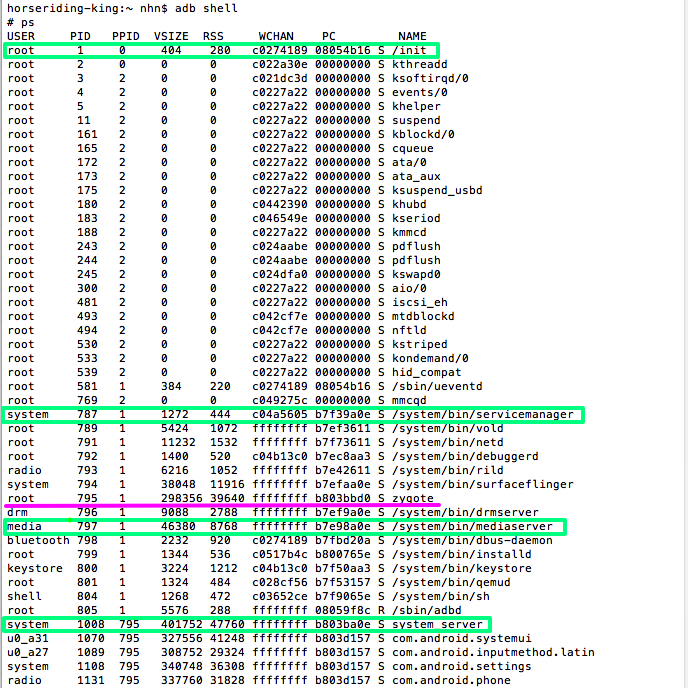
\includegraphics[scale=0.7]{ps}
Binder의 기본 내용은 \url{http://helloworld.naver.com/helloworld/47656}에 간략하게 나와있다.
책으로는 위키북스에서 나온 ``인사이드 안드로이드''나 한빛미디어에서 나온 ``안드로이드의 모든 것 분석과 포팅''을 참고해 보자.\\
Binder IPC, Binder RPC 헷갈린다.

%http://www.angryredplanet.com/~hackbod/openbinder/docs/html/BinderIPCMechanism.html
%http://rts.lab.asu.edu/web_438/project_final/Talk%208%20AndroidArc_Binder.pdf

시스템 서비스는 항상 바인더 통신을 한다.


binder call back 서비스 만들어보자.



% https://thenewcircle.com/s/post/1340/Deep_Dive_Into_Binder_Presentation.htm

binder Thread Pool은 최대 16개. 시작하면서 2개가 생성이 되고(ViewRootImpl, ActivityThread\$ApplicationThread 용도) 필요하면 추가한다. binding이 많다면 timeout 날 수 있다.
/frameworks/native/libs/binder/ProcessState.cpp에서 open\_driver 함수를 보자.
(ZygoteInit.main이 실행되고, RuntimeInit.ZygoteInitNative에서 app\_main.cpp에서 AppRuntiume.onZygoteInit에서 호출한다.)
surfaceflinger는 최대 4개로 세팅하고 있다.(setThreadPollMaxTheadCount 함수 호출)

stub 호출시 handler를 주로 사용한다.(UI 업데이트 필요할 때)
클라이언트는 proxy, 서버는 stub이다.
systemserver: ActivityManagerService, PackageManagerService, LocationManagerService, AlarmManagerService, ConnectivityService, SensorService, WifiService
/system/bin/mediaserver : AudioFlinger, CameraService, MediaPlayerService, AudioPolicyService 네이티브 시스템 서비스로 cpp로 되어 있다.
/system/bin/surfaceflinger: SurfaceFlinger 네이티브 시스템 서비스로 cpp로 되어 있다. 

init.rc에 보면 surfaceflinger가 먼저 실행되고, mediaserver가 실행된다.
systemserver는 zygote에서 실행
servicemanager
\end{comment}

\chapter{시스템 서비스}
% http://www.vogella.com/tutorials/AndroidServices/article.html
%안드로이드에서는 API와 internal에서 시스템 서비스를 구분하는 것이 약간 차이가 있다. 두 가지를 동일한 것으로 이해하고 있다면 혼동이 생기므로, 차이를 정리하고 넘어가도록 하자.
시스템 서비스는 앱에서 사용하는 정보와 기능을 시스템에서 Binder를 통해서 제공하는 것이다.
Service 컴포넌트처럼 따로 시작할 필요가 없고, 시스템에서 이미 존재하고 실행 중인 서비스를 앱에서 이용한다.
시스템 서비스는 대부분 자바로 작성되어 있고, 일부만 C/C++로 작성되어 있다.\\

아래는 adb shell에서 ps를 실행한 결과이다.
\begin{lstlisting}[frame=single] 
shell@EF56S:/ $ ps
USER     PID   PPID  VSIZE  RSS     WCHAN    PC         NAME
root      1     0     788    600   ffffffff 00000000 S /init
root      2     0     0      0     ffffffff 00000000 S kthreadd
root      3     2     0      0     ffffffff 00000000 S ksoftirqd/0
root      6     2     0      0     ffffffff 00000000 D kworker/u:0
root      7     2     0      0     ffffffff 00000000 D kworker/u:0H
root      8     2     0      0     ffffffff 00000000 S migration/0
root      21    2     0      0     ffffffff 00000000 S khelper
root      22    2     0      0     ffffffff 00000000 S netns
root      28    2     0      0     ffffffff 00000000 S modem_notifier
root      29    2     0      0     ffffffff 00000000 S smd_channel_clo
root      30    2     0      0     ffffffff 00000000 S smsm_cb_wq
root      32    2     0      0     ffffffff 00000000 S rpm-smd
root      33    2     0      0     ffffffff 00000000 S kworker/u:1H
root      34    2     0      0     ffffffff 00000000 S mpm
root      49    2     0      0     ffffffff 00000000 S sync_supers
root      50    2     0      0     ffffffff 00000000 S bdi-default
root      51    2     0      0     ffffffff 00000000 S kblockd
root      52    2     0      0     ffffffff 00000000 S system
root      53    2     0      0     ffffffff 00000000 S khubd
...
root      340   1     1484   4     ffffffff 00000000 S /sbin/healthd
system    341   1     1428   588   ffffffff 00000000 S /system/bin/servicemanager
root      342   1     4892   808   ffffffff 00000000 S /system/bin/vold
system    344   1     2568   724   ffffffff 00000000 S /system/bin/rfs_access
system    347   1     3820   1044  ffffffff 00000000 S /system/bin/qseecomd
root      350   1     10648  1488  ffffffff 00000000 S /system/bin/netd
root      351   1     8020   1052  ffffffff 00000000 S /system/bin/debuggerd
root      352   1     1448   580   ffffffff 00000000 S /system/bin/pam_server
radio     353   1     27984  3052  ffffffff 00000000 S /system/bin/rild
system    354   1     121284 5324  ffffffff 00000000 S /system/bin/surfaceflinger
root      355   1     861344 19116 ffffffff 00000000 S zygote
drm       356   1     28192  2748  ffffffff 00000000 S /system/bin/drmserver
media     357   1     69708  7484  ffffffff 00000000 S /system/bin/mediaserver
install   358   1     1412   704   ffffffff 00000000 S /system/bin/installd
keystore  360   1     3736   872   ffffffff 00000000 S /system/bin/keystore
...
shell     477   1     5700   244   ffffffff 00000000 S /sbin/adbd
...
system    1192  355   1014224 74416 ffffffff 00000000 S system_server
u0_a12    1385  355   1082344 150852 ffffffff 00000000 S com.android.systemui
radio     1619  355   913032 24116 ffffffff 00000000 S com.android.phone
u0_a134   1661  355   870396 21168 ffffffff 00000000 S com.skt.tbmon
u0_a50    1675  355   870900 20432 ffffffff 00000000 S com.skt.apra
...
u0_a110   1780  355   960648 126336 ffffffff 00000000 S com.pantech.launcher2
u0_a197   1881  355   869196 16148 ffffffff 00000000 S com.android.smspush
u0_a9     1976  355   1068200 37924 ffffffff 00000000 S com.google.android.gms
u0_a9     2011  355   939400 32092 ffffffff 00000000 S com.google.process.gapps
u0_a9     2063  355   948572 36028 ffffffff 00000000 S com.google.process.location
u0_a31    2330  355   881220 21224 ffffffff 00000000 S com.skt.skaf.OA00199800
bluetooth 2667  355   915620 21268 ffffffff 00000000 S com.android.bluetooth
system    2688  355   982224 47708 ffffffff 00000000 S com.pantech.powersaver
u0_a57    3025  355   914296 21860 ffffffff 00000000 S com.android.calendar
u0_a63    3304  355   880016 18668 ffffffff 00000000 S com.skt.iwlan:remote
system    3370  355   877760 24112 ffffffff 00000000 S com.skt.tmode
system    3713  355   872376 16280 ffffffff 00000000 S com.qualcomm.atfwd
u0_a65    4640  355   883112 19772 ffffffff 00000000 S com.android.deskclock
u0_a57    4782  355   887760 21420 ffffffff 00000000 S com.android.calendar:remote
u0_a139   7531  355   873552 21924 ffffffff 00000000 S android.process.acore
u0_a15    12207 355   906192 25548 ffffffff 00000000 S com.android.vending
...
\end{lstlisting}

여기서 /system/bin/mediaserver, /system/bin/surfaceflinger 2개가 C/C++로 작성된 시스템 서비스이고, 앱에서 일반적으로 직접 접근해서 사용하지 않는다.
%롤리팝에 추가된 CameraManager가 하나의 예외이다.
/system/bin/mediaserver는 MediaPlayer, MediaRecorder, Camera 같은 클래스에서 사용하거나, AudioService 같은 자바로 작성된 시스템 서비스에서 접근한다.\footnote{AudioService에서는 AudioSystem 클래스를 통해 네이티브에 접근한다.}
/system/bin/surfaceflinger는 WindowManagerService에서 접근해서 화면에 반영하고 있다.\\

\section{시스템 서비스 기본}
시스템 서비스는 자바로 작성된 시스템 서비스가 많은데 이것들은 system\_server 프로세스에서 동작한다.
Context에는 getSystemService(String name) 메서드가 있어서, 리턴 결과는 시스템 서비스를 래핑한 것이고 사용 시에 반드시 캐스팅해서 사용한다.
시스템 서비스는 많은 경우 Binder Proxy를 래핑하고서 -Manager 식의 네이밍을 가진다. 그리고 -Manager에서는 Stub의 모든 public 메서드를 다 사용할 수 있는 것은 아니다.
예를 들어, ActivityManager에서 startActivity() 메서드를 실행할 수는 없다.
아래 표를 보도록 하자. 일반적인 네이밍 패턴에 맞는 것도 많지만 아닌 것도 여럿 있다(롤리팝 기준).
\newpage
% com.android.server.SystemServer 참고
%\newgeometry{left=2cm,bottom=2cm}
\scalebox{0.73}{
\begin{tabular}[fontsize=\tiny]{|l|l|l|l|l|} \hline
Context 상수 & getSystemService 결과 & 인터페이스 & Stub 구현 \\ \hline
ACCESSIBILITY\_SERVICE & AccessibilityManager & IAccessibilityManager & AccessibilityManagerService  \\ \hline
ACCOUNT\_SERVICE & AccountManager & IAccountManager & AccountManagerService \\ \hline
ACTIVITY\_SERVICE & ActivityManager & IActivityManager & ActivityManagerService \\ \hline
ALARM\_SERVICE & AlarmManager & IAlarmManager & AlarmManagerService \\ \hline
APPWIDGET\_SERVICE	& AppWidgetManager & IAppWidgetService & AppWidgetService \\ \hline
APP\_OPS\_SERVICE & AppOpsManager & IAppOpsService & AppOpsService \\ \hline
AUDIO\_SERVICE & AudioManager & IAudioService & AudioService \\ \hline
BATTERY\_SERVICE	 & BatteryManager & IBatteryPropertiesRegistrar & IBatteryPropertiesRegistrar.cpp \\ \hline
BLUETOOTH\_SERVICE & BluetoothAdapter & IBluetoothManager & BluetoothManagerService \\ \hline
CAMERA\_SERVICE & CameraManager & ICameraService & CameraService.cpp \\ \hline 
CAPTIONING\_SERVICE & CaptioningManager & 없음 & ContentResolver 사용 \\ \hline
CLIPBOARD\_SERVICE & ClipboardManager & IClipboard & ClipboardService \\ \hline
CONNECTIVITY\_SERVICE & ConnectivityManager & IConnectivityManager & ConnectivityService \\ \hline
CONSUMER\_IR\_SERVICE & ConsumerIrManager & IConsumerIrService & ConsumerIrService \\ \hline
DEVICE\_POLICY\_SERVICE & DevicePolicyManager & IDevicePolicyManager & DevicePolicyManagerService \\ \hline
DISPLAY\_SERVICE	& DisplayManager & IDisplayManager & DisplayManagerService \\ \hline
DOWNLOAD\_SERVICE & DownloadManager & 없음 & ContentResolver 사용 \\ \hline
DROPBOX\_SERVICE	& DropBoxManager & IDropBoxManagerService &  DropBoxManagerService\\ \hline
INPUT\_METHOD\_SERVICE	 & InputMethodManager & IInputMethodManager & InputMethodManagerService \\ \hline
INPUT\_SERVICE & InputManager & IInputManager & InputManagerService \\ \hline
JOB\_SCHEDULER\_SERVICE & JobScheduler & IJobScheduler & JobSchedulerService \\ \hline
KEYGUARD\_SERVICE	 & KeyguardManager & 없음 & 없음 \\ \hline
LAUNCHER\_APPS\_SERVICE & LauncherApps &  ILauncherApps & LauncherAppsService \\ \hline
\makecell[l]{LAYOUT\_INFLATER\\ \_SERVICE} & LayoutInflater & 없음 & 없음 \\ \hline
LOCATION\_SERVICE	 & LocationManager & ILocationManager & LocationManagerService \\ \hline
\makecell[l]{MEDIA\_PROJECTION\\ \_SERVICE}	 & MediaProjectionManager  & IMediaProjectionManager & MediaProjectionManagerService \\ \hline
MEDIA\_ROUTER\_SERVICE	 & MediaRouter & IMediaRouterService & MediaRouterService \\ \hline
MEDIA\_SESSION\_SERVICE & MediaSessionManager & ISessionManager & MediaSessionService\\ \hline
NFC\_SERVICE	& NfcManager & 없음 & 없음 \\ \hline
NOTIFICATION\_SERVICE & NotificationManager & INotificationManager & NotificationManagerService \\ \hline
NSD\_SERVICE	& NsdManager & INsdManager & NsdService \\ \hline
POWER\_SERVICE & PowerManager & IPowerManager & PowerManagerService \\ \hline
PRINT\_SERVICE &	PrintManager & IPrintManager & PrintManagerService\\ \hline
RESTRICTIONS\_SERVICE & RestrictionsManager &  IRestrictionsManager  & RestrictionsManagerService \\ \hline
SEARCH\_SERVICE & SearchManager & ISearchManager & SearchManagerService \\ \hline
SENSOR\_SERVICE & SensorManager & 없음 & 없음 \\ \hline
STORAGE\_SERVICE	& StorageManager & IMountService & MountService\\ \hline
TELECOM\_SERVICE	& TelecomManager &  ITelecomService &  TelecomServiceImpl\\ \hline
TELEPHONY\_SERVICE & TelephonyManager & ITelephonyRegistry & TelephonyRegistry \\ \hline
\makecell[l]{TEXT\_SERVICES\_MANAGER\\ \_SERVICE} & TextServicesManager & ITextServicesManager & TextServicesManagerService \\ \hline
TV\_INPUT\_SERVICE	 & TvInputManager &  ITvInputManager & TvInputManagerService \\ \hline
UI\_MODE\_SERVICE	& UiModeManager & IUiModeManager & UiModeManagerService \\ \hline
USB\_SERVICE	 & UsbManager & IUsbManager & UsbService \\ \hline
USER\_SERVICE	 & UserManager & IUserManager & UserManagerService \\ \hline
VIBRATOR\_SERVICE & Vibrator & IVibratorService & VibratorService \\ \hline
WALLPAPER\_SERVICE & WallpaperManager & IWallpaperManager & WallpaperManagerService \\ \hline
WIFI\_P2P\_SERVICE	 & WifiP2pManager & IWifiP2pManager & WifiP2pService \\ \hline
WIFI\_SERVICE & WifiManager & IWifiManager & WifiService \\ \hline
WINDOW\_SERVICE & WindowManager & IWindowManager & WindowManagerService \\ \hline
\end{tabular}
}
%\restoregeometry

4.X 이후에도 여러 서비스가 추가되어서 생소한 것들이 있는데 굳이 살펴보지는 않겠다.
하나하나 보는 것보다는 전체적으로 특기할 만한 내용 위주로 보도록 하자.
\begin{itemize}
\item getSystemService()의 결과로서 -Manager 네이밍을 따르지 않는 것은 JobScheduler, LauncherApps, LayoutInflater, MediaRouter, Vibrator 4가지이다. 

\item 인터페이스 이름은 getSystemService() 결과 클래스에 일반적으로는 앞에 I를 붙이지만, 예외 케이스가 너무 많다. 
Manager 자리에 Service가 붙기도 하고, Manager가 빠지기도 하고 ManagerService로 끝나기도 한다. 

\item 안드로이드 컴포넌트와 연관되어 있기 때문에 시스템 서비스 가운데 가장 많이 참고해야 하는 ActivityManagerService는 추상 클래스인 ActivityManagerNative를 상속한다. ActivityManagerNative는 IActivityManager의 Stub 구현이 아니라, Binder를 상속한 IActivityManager 인터페이스 구현이다. 그래서 asInterface()나 onTransact() 메서드 등이 직접 구현되어 있다.

\item LayoutInflator는 Binder 통신을 하는 것이 아니고, PolicyManager.makeNewLayoutInflater()를 통해  com.android.internal.policy.impl.PhoneLayoutInflator를 가져온다.
사용할 때 LayoutInflator를 가져오는 메서드는 3가지가 있다.
\begin{itemize}
\item (LayoutInflator) Context.getSystemService(Context.LAYOUT\_INFLATER\_SERV\-ICE)
\item LayoutInflator.from(Context context)
\item Activity의 getLayoutInflator()
\end{itemize}
두 번째와 세 번째가 내부적으로 첫 번째 메서드를 다시 호출하는데, 일반적으로 간편하게 많이 사용하는 것은 두 번째 메서드이다.

\item CameraService는 네이티브로 작성되어 있다. Binder 통신은 마샬링, 언마샬링만 하면 되기 때문에 네이티브에서 언마샬링해서 요청을 처리하는 식이다.

\item BatteryManager는 기존에는 ACTION\_BATTERY\_CHANGED Intent에서 쓰이는 문자열과 숫자 상수만을 정의하고 있었는데, 롤리팝에서 배터리와 충전 속성을 조회하는 메서드가 추가되었다.

\item DownloadService는 별도 프로세스인 android.process.media에서 실행된다. 
DownloadManager는 ContentResolver를 통해 DB에 쌓는 역할만 한다.
DownloadService는 프레임워크 소스에서 packages/providers/DownloadProvider 디렉터리에 있는 Service 컴포넌트이다. 
DownloadReceiver에서 Intent.ACTION\_BOOT\_COMPLETED, Intent.ACTION\_MEDIA\_MOUNTED, C\-onnectivityManager.CONNECTIVITY\_ACTIO\-N(연결될 때)와 내부적으로 쓰는 Action인 ACTION\-\_RETRY Broadcast 이벤트 발생 시에 DownloadService를 시작한다.

\item 추상 클래스인 SensorManager의 실제 구현은 android.hardware.SystemSensorManager이다. 
ContextImpl에서 처음 SensorManager를 Service Map에 넣을 때, SensorManager의 생성자에서는 네이티브에서 Sensor 목록을 로딩한다.

\item NfcManager는 NfcAdapter를 얻기 위한 용도로, getDefaultAdapter() 메서드 하나만 있다. NfcService의 내부 클래스인 NfcAdapterService에서 INfcAdapter.Stub을 구현하고, NfcAdapter에서는 여기에 접근한다.

\item InputMethodManager는 주로 EditText에 소프트 키보드를 연결하는 데 사용된다. Stub 구현은 InputMethodManagerService인데, 이와 별도로 InputMethodService 클래스도 있다. 
전자는 system\_server에서 실행되는 클래스이고, 후자는 Service를 상속하고 소프트 키보드를 구현할 때 사용하는 클래스이다.

\item 롤리팝에는 com.android.server.SystemService가 추가되어서 시스템 서비스  클래스는 이를 상속하고 Stub 구현은 내부 클래스에서 하고 있다.\\
\begin{tabular}[fontsize=\tiny]{|l|l|} \hline
Service & Stub 구현 내부 클래스 \\ \hline
JobSchedulerService & JobSchedulerStub \\ \hline
LauncherAppsService & LauncherAppsImpl \\ \hline
MediaSessionService & SessionManagerImpl \\ \hline
RestrictionsManagerService & RestrictionsManagerImpl \\ \hline
TvInputManagerService & BinderService \\ \hline
\end{tabular}
\end{itemize}

Binder Stub 구현이 없는 것은 실제로는 Binder 통신을 하는 건 아니다.
서비스명이 DOWNLOAD\_SERVICE나 LAYOUT\_INFLATER\_SERVICE 같은 것은 편의상 시스템 서비스일 뿐이다.\\

Binder Stub 구현은 어느 프로세스에서 돌아가고 있을까? Binder Stub이 각각 따로 프로세스로 실행되는 것이 아닐까 생각할 수도 있지만, 앞에서도 여러 차례 얘기한 system\_server 프로세스에서 실행되고 있다(예외로 CameraService는 /system/bin/mediaserver 프로세스에서 실행된다).			
system\_server에서 여러 시스템 서비스를 제공하고, 이를 다른 앱에서 호출하는 것으로 이해하면 된다.\\

여기서 하나 질문을 해보자. Service 컴포넌트와 시스템 서비스는 어떻게 다를까?
이 내용을 생각해보면 다음과 같이 정리해볼 수 있다.
\begin{itemize}
\item 시스템 서비스는 /system/bin/servicemanager에 Stub을 등록하고 필요할 때 가져와서 사용하고, Service 컴포넌트는 ActivityManagerService의 내부 목록으로 유지된다(젤리빈부터 ActiveServices에 위임)
\item 시스템 서비스는 Stub 자체로 구현하지만, Service 컴포넌트는 android.os.Service를 상속하고 내부에 Stub을 구현한다.
\end{itemize}

이제 프레임워크 소스를 보자.
/system/bin/servicemanager 프로세스에 Stub을 등록하는 내용은 /frameworks/base/services/java/com/android/server/SystemServer.java\footnote{system\_server 프로세스의 메인 클래스이다.}에서 내부 클래스인 ServerThread의 initAndLoop() 메서드에서 볼 수 있다.

\begin{lstlisting}[frame=single, caption=SystemServer.java] 
	display = new DisplayManagerService(context, wmHandler);
	ServiceManager.addService(Context.DISPLAY_SERVICE, display, true);
	
	telephonyRegistry = new TelephonyRegistry(context);
	ServiceManager.addService("telephony.registry", telephonyRegistry);
	
	ServiceManager.addService("scheduling_policy", 
		new SchedulingPolicyService());
		
	...
	ActivityManagerService.setSystemProcess(); // (1)
		
	...
	ServiceManager.addService("battery", battery);
	
	vibrator = new VibratorService(context);
	ServiceManager.addService("vibrator", vibrator);
	
	...
	inputManager = new InputManagerService(context, wmHandler);
	wm = WindowManagerService.main(context, power, display, inputManager,
	        wmHandler, factoryTest != SystemServer.FACTORY_TEST_LOW_LEVEL,
	        !firstBoot, onlyCore);
	ServiceManager.addService(Context.WINDOW_SERVICE, wm);
	ServiceManager.addService(Context.INPUT_SERVICE, inputManager);
\end{lstlisting}	    
ServiceManager.addService() 메서드를 통해서 여러 Stub을 등록하는 것을 볼 수 있다.
% /frameworks/base/core/java/android/os/ServiceManager.java
여기서 보면 ActivityManagerService 등록이 눈에 띄지 않는데, 관련 코드는 ActivityManagerService 안에 있다. 
11라인(1)에서 ActivityManagerService.setSystemProcess() 호출이 있는데, 여기서 자기 자신을 등록하고 있다.
\begin{lstlisting}[frame=single, caption=ActivityManagerService.java] 
   public static void setSystemProcess() {
        try {
            ActivityManagerService m = mSelf;

            ServiceManager.addService(Context.ACTIVITY_SERVICE, m, true);
            ServiceManager.addService(ProcessStats.SERVICE_NAME, m.mProcessStats);
            ServiceManager.addService("meminfo", new MemBinder(m));
            ServiceManager.addService("gfxinfo", new GraphicsBinder(m));
            ServiceManager.addService("dbinfo", new DbBinder(m));
            if (MONITOR_CPU_USAGE) {
                ServiceManager.addService("cpuinfo", new CpuBinder(m));
            }
            ServiceManager.addService("permission", new PermissionController(m));
 			...
        } catch (PackageManager.NameNotFoundException e) {
            throw new RuntimeException(
                    "Unable to find android system package", e);
        }
    }
\end{lstlisting}	    


\begin{comment}
ViewRootImpl에서 onConfigurationChanged 이후에 measure 호출하고 있다. 사이즈 조정하기 좋은 곳이 onConfigurationChanged 메서드이다.

ActivityManagerService, WindowManagerService, PackageManagerService, LocationManagerService, AlarmManagerService, PowerManagerService, BackupManagerService, InputManagerService, AppWidgetService, AudioService, ConnectivityService, VibratorService 등 자바 시스템 서비스로 Binder Stub을 구현하고 있고, system\_server 프로세스에서 실행된다.\\
\end{comment}

시스템 서비스를 사용하는 쪽에서는 어떨까. 매번 /system/bin/servicemanager에서 조회해서 호출하는가 하면 그렇지 않다.
바로 ContextImpl의 정적 초기화 블록(static initializer block) 안에서 처음 생성될 때 단 한번만 매핑하고 사용한다.
참고로 마시멜로에서는 아래 로직을 SystemServiceRegistry 클래스에 위임하였다.
\begin{lstlisting}[frame=single, caption=ContextImpl.java] 
  private static final HashMap<String, ServiceFetcher> SYSTEM_SERVICE_MAP =
            new HashMap<String, ServiceFetcher>();

  private static int sNextPerContextServiceCacheIndex = 0;
  private static void registerService(String serviceName, ServiceFetcher fetcher) {
      if (!(fetcher instanceof StaticServiceFetcher)) {
          fetcher.mContextCacheIndex = sNextPerContextServiceCacheIndex++;
      }
      SYSTEM_SERVICE_MAP.put(serviceName, fetcher);
  }
    
  static {
        registerService(ACCESSIBILITY_SERVICE, new ServiceFetcher() {
                public Object getService(ContextImpl ctx) {
                    return AccessibilityManager.getInstance(ctx);
                }});

        registerService(ACCOUNT_SERVICE, new ServiceFetcher() {
                public Object createService(ContextImpl ctx) {
                    IBinder b = ServiceManager.getService(ACCOUNT_SERVICE);
                    IAccountManager service = IAccountManager.Stub.asInterface(b);
                    return new AccountManager(ctx, service); // (1)
                }});

        registerService(ACTIVITY_SERVICE, new ServiceFetcher() {
                public Object createService(ContextImpl ctx) {
                    return new ActivityManager(ctx.getOuterContext(), 
                    	ctx.mMainThread.getHandler());
                }});

        registerService(ALARM_SERVICE, new ServiceFetcher() {
                public Object createService(ContextImpl ctx) {
                    IBinder b = ServiceManager.getService(ALARM_SERVICE);
                    IAlarmManager service = IAlarmManager.Stub.asInterface(b);
                    return new AlarmManager(service, ctx); // (2)
                }});
		...
        registerService(LAYOUT_INFLATER_SERVICE, new ServiceFetcher() {
                public Object createService(ContextImpl ctx) {
                    return PolicyManager.makeNewLayoutInflater(
                    	ctx.getOuterContext());
                }});

        registerService(LOCATION_SERVICE, new ServiceFetcher() {
                public Object createService(ContextImpl ctx) {
                    IBinder b = ServiceManager.getService(LOCATION_SERVICE);
                    return new LocationManager(ctx, 
                    	ILocationManager.Stub.asInterface(b));
                }});

        registerService(NETWORK_POLICY_SERVICE, new ServiceFetcher() {
            @Override
            public Object createService(ContextImpl ctx) {
                return new NetworkPolicyManager(
                	INetworkPolicyManager.Stub.asInterface(
                    ServiceManager.getService(NETWORK_POLICY_SERVICE)));
            }
        });
		...
        registerService(POWER_SERVICE, new ServiceFetcher() {
                public Object createService(ContextImpl ctx) {
                    IBinder b = ServiceManager.getService(POWER_SERVICE);
                    IPowerManager service = IPowerManager.Stub.asInterface(b);
                    return new PowerManager(ctx.getOuterContext(),
                            service, ctx.mMainThread.getHandler());
                }});
		...
        registerService(TELEPHONY_SERVICE, new ServiceFetcher() {
                public Object createService(ContextImpl ctx) {
                    return new TelephonyManager(ctx.getOuterContext());
                }});

        registerService(VIBRATOR_SERVICE, new ServiceFetcher() {
                public Object createService(ContextImpl ctx) {
                    return new SystemVibrator(ctx);
                }});
		...
    }
\end{lstlisting}
22라인(1)과 35라인(2)에서 AccountManager나 AlarmManager를 보면 Binder Proxy를 감싼 객체임을 바로 알 수 있는데, 대부분 이와 유사하게 되어 있다.

% http://developer.android.com/reference/android/content/Context.html

\section{dumpsys 명령어}\label{sec:dumpsys}
adb shell에서 가장 많이 실행하는 명령어 가운데 하나가 앞에서도 여러 차례 언급한 dumpsys이다. 
dumpsys 명령어만 사용하면 너무 많은 정보가 나오고, dumpsys activity나 dumpsys package처럼 원하는 정보에 한정해서 보는 것이 좋다.
그런데 dumpsys 다음에 들어가는 옵션 항목은 어떤 것이 있을까? 
이를 아는 방법은 바로 shell에서 service list\footnote{/frameworks/native/cmds/service/service.cpp 소스를 참고하자.}를 실행하는 것이다.
% Android Graphics Architecture.pdf 참고할 것
\begin{lstlisting}[frame=single] 
# service list
Found 65 services:
0	phone: [com.android.internal.telephony.ITelephony]
1	iphonesubinfo: [com.android.internal.telephony.IPhoneSubInfo]
2	simphonebook: [com.android.internal.telephony.IIccPhoneBook]
3	isms: [com.android.internal.telephony.ISms]
4	commontime_management: []
5	samplingprofiler: []
6	diskstats: []
7	appwidget: [com.android.internal.appwidget.IAppWidgetService]
8	backup: [android.app.backup.IBackupManager]
9	uimode: [android.app.IUiModeManager]
10	serial: [android.hardware.ISerialManager]
11	usb: [android.hardware.usb.IUsbManager]
12	audio: [android.media.IAudioService]
13	wallpaper: [android.app.IWallpaperManager]
14	dropbox: [com.android.internal.os.IDropBoxManagerService]
15	search: [android.app.ISearchManager]
16	country_detector: [android.location.ICountryDetector]
17	location: [android.location.ILocationManager]
18	devicestoragemonitor: []
19	notification: [android.app.INotificationManager]
20	updatelock: [android.os.IUpdateLock]
21	throttle: [android.net.IThrottleManager]
22	servicediscovery: [android.net.nsd.INsdManager]
23	connectivity: [android.net.IConnectivityManager]
24	wifi: [android.net.wifi.IWifiManager]
25	wifip2p: [android.net.wifi.p2p.IWifiP2pManager]
26	netpolicy: [android.net.INetworkPolicyManager]
27	netstats: [android.net.INetworkStatsService]
28	textservices: [com.android.internal.textservice.ITextServicesManager]
29	network_management: [android.os.INetworkManagementService]
30	clipboard: [android.content.IClipboard]
31	statusbar: [com.android.internal.statusbar.IStatusBarService]
32	device_policy: [android.app.admin.IDevicePolicyManager]
33	lock_settings: [com.android.internal.widget.ILockSettings]
34	mount: [IMountService]
35	accessibility: [android.view.accessibility.IAccessibilityManager]
36	input_method: [com.android.internal.view.IInputMethodManager]
37	input: [android.hardware.input.IInputManager]
38	window: [android.view.IWindowManager]
39	alarm: [android.app.IAlarmManager]
40	vibrator: [android.os.IVibratorService]
41	battery: []
42	hardware: [android.os.IHardwareService]
43	content: [android.content.IContentService]
44	account: [android.accounts.IAccountManager]
45	permission: [android.os.IPermissionController]
46	cpuinfo: []
47	dbinfo: []
48	gfxinfo: []
49	meminfo: []
50	activity: [android.app.IActivityManager]
51	package: [android.content.pm.IPackageManager]
52	scheduling_policy: [android.os.ISchedulingPolicyService]
53	telephony.registry: [com.android.internal.telephony.ITelephonyRegistry]
54	usagestats: [com.android.internal.app.IUsageStats]
55	batteryinfo: [com.android.internal.app.IBatteryStats]
56	power: [android.os.IPowerManager]
57	entropy: []
58	sensorservice: [android.gui.SensorServer]
59	media.audio_policy: [android.media.IAudioPolicyService]
60	media.camera: [android.hardware.ICameraService]
61	media.player: [android.media.IMediaPlayerService]
62	media.audio_flinger: [android.media.IAudioFlinger]
63	SurfaceFlinger: [android.ui.ISurfaceComposer]
64	drm.drmManager: [drm.IDrmManagerService]
\end{lstlisting}

각 라인에서 clone(:) 앞에 있는 문자열이 바로 dumpsys 다음에 올 수 있는 값들이다.
이 항목들이 dump할 수 있다는 것인데, 이 항목들은 무엇인가 하면 /system/bin/servicemanager에 등록된 시스템 서비스 목록이다.
항목의 어떤 내용을 출력하는지는 ActivityManagerService, AlarmManagerService 등 시스템 서비스 클래스의 dump() 메서드를 보면 된다. 
앞에서 안드로이드 버전마다 dumpsys 결과가 차이가 있다고 언급하였는데, 버전이 올라가면서 dump() 메서드는 클래스에 새로 추가된 여러 멤버 변수값과 함께 더 상세한 내용을 출력하기 때문이다.\\

service list 결과에서 clone(:) 뒤에 [] 공백으로 나오는 것은 Binder Stub을 등록한 것이 아닌 Binder를 만들어서 일부러 등록한 것으로, dump 용도의 서비스이다.
예를 들어, dumpsys meminfo 같은 명령을 쓰는 경우가 있는데, meminfo 관련 시스템 서비스는 없다. 
위에서 ActivityManagerService.setSystemProcess() 메서드의 7라인을 보면 ServiceManager.addService(``meminfo'', new MemBinder(m))가 있다.
이제 ActivityManagerService의 정적 내부 클래스인 MemBinder를 찾아보면 별게 없고, Binder를 상속하고 dump() 메서드가 유일한 메서드일 뿐이다.
\begin{lstlisting}[frame=single]
    static class MemBinder extends Binder {
        ActivityManagerService mActivityManagerService;
        MemBinder(ActivityManagerService activityManagerService) {
            mActivityManagerService = activityManagerService;
        }

        @Override
        protected void dump(FileDescriptor fd, PrintWriter pw, String[] args) {
            if (mActivityManagerService.checkCallingPermission(
            		android.Manifest.permission.DUMP)
                    != PackageManager.PERMISSION_GRANTED) {
                pw.println("Permission Denial: can't dump meminfo from from pid="
                	+ Binder.getCallingPid() + ", uid=" + Binder.getCallingUid()
                    + " without permission " + android.Manifest.permission.DUMP);
                return;
            }

            mActivityManagerService.dumpApplicationMemoryUsage(fd, pw, "  ", args, false, null);
        }
    }
\end{lstlisting}
이것이 동작하는 이유는 Binder 클래스에도 onTransact() 메서드가 정의되어 있고,
여기서 DUMP\_TRANSAC\-TION code을 처리하기 때문이다.
그리고 시스템 서비스 Stub에서는 onTransact() 메서드 맨 아래에 super.onTransact(code, data, reply, flags)를 호출하고 있다.

\begin{lstlisting}[frame=single]
   protected boolean onTransact(int code, Parcel data, Parcel reply,
            int flags) throws RemoteException {
        if (code == INTERFACE_TRANSACTION) {
            reply.writeString(getInterfaceDescriptor());
            return true;
        } else if (code == DUMP_TRANSACTION) {
            ParcelFileDescriptor fd = data.readFileDescriptor();
            String[] args = data.readStringArray();
            if (fd != null) {
                try {
                    dump(fd.getFileDescriptor(), args);
                } finally {
                    try {
                        fd.close();
                    } catch (IOException e) {
                    }
                }
            }
            if (reply != null) {
                reply.writeNoException();
            } else {
                StrictMode.clearGatheredViolations();
            }
            return true;
        }
        return false;
    }
\end{lstlisting}

dumpsys activity를 하면 ActivityManagerService가 워낙 많은 정보를 가지고 있기 때문에 보여주는 것이 적지 않다.
정작 필요한 정보를 찾기 위해서 추가로 명령을 덧붙이는 게 좋다. -h 옵션을 사용해서 추가로 덧붙여 쓸 수 있는 것을 알아보자(모든 서비스가 -h 옵션을 쓸 수 있는 것은 아니다).
아래는 activity와 package, meminfo에 쓸 수 있는 것을 조회한 것이다.
\begin{lstlisting}[frame=single]
shell@EF56S:/ $ dumpsys activity -h 
Activity manager dump options:
  [-a] [-c] [-h] [cmd] ...
  cmd may be one of:
    a[ctivities]: activity stack state
    b[roadcasts] [PACKAGE_NAME] [history [-s]]: broadcast state
    i[ntents] [PACKAGE_NAME]: pending intent state
    p[rocesses] [PACKAGE_NAME]: process state
    o[om]: out of memory management
    prov[iders] [COMP_SPEC ...]: content provider state
    provider [COMP_SPEC]: provider client-side state
    s[ervices] [COMP_SPEC ...]: service state
    service [COMP_SPEC]: service client-side state
    package [PACKAGE_NAME]: all state related to given package
    all: dump all activities
    top: dump the top activity
  cmd may also be a COMP_SPEC to dump activities.
  COMP_SPEC may be a component name (com.foo/.myApp),
    a partial substring in a component name, a
    hex object identifier.
  -a: include all available server state.
  -c: include client state.
  
shell@EF56S:/ $ dumpsys package -h                                             
Package manager dump options:
  [-h] [-f] [cmd] ...
    -f: print details of intent filters
    -h: print this help
  cmd may be one of:
    l[ibraries]: list known shared libraries
    f[ibraries]: list device features
    r[esolvers]: dump intent resolvers
    perm[issions]: dump permissions
    pref[erred]: print preferred package settings
    preferred-xml [--full]: print preferred package settings as xml
    prov[iders]: dump content providers
    p[ackages]: dump installed packages
    s[hared-users]: dump shared user IDs
    m[essages]: print collected runtime messages
    v[erifiers]: print package verifier info
    <package.name>: info about given package
    k[eysets]: print known keysets
    
shell@EF56S:/ $ dumpsys meminfo -h
meminfo dump options: [-a] [-d] [-c] [--oom] [process]
  -a: include all available information for each process.
  -d: include dalvik details when dumping process details.
  -c: dump in a compact machine-parseable representation.
  --oom: only show processes organized by oom adj.
  --local: only collect details locally, don't call process.
If [process] is specified it can be the name or 
pid of a specific process to dump.
\end{lstlisting}

Debug 클래스에는 dumpService() 메서드도 있다. 
이 메서드로 파일에 dumpsys 결과를 출력할 수 있는데, 메서드를 사용하기 위해서는 android.permission.DUMP 퍼미션이 필요하고 이 퍼미션은 시스템 앱에서만 사용할 수 있다. 따라서 일반 앱에서는 Debug.dumpService()는 사용할 수 없다.

\begin{comment}
코드 상에서도 dump를 생성하고 싶은 경우가 있다.
아래는 안드로이드 소스에서 /packages/apps/Settings 앱에서 Debug.dumpService(String name, FileDescriptor fd, String[] args) 메서드를 사용한 예이다. (android.permission.DUMP 퍼미션은 필요하다.)
\begin{lstlisting}[frame=single]
    ComponentName comp = new ComponentName(mServiceItem.mServiceInfo.packageName,
            mServiceItem.mServiceInfo.name);
    File filename = getActivity().getFileStreamPath("service_dump.txt");
    FileOutputStream output = null;
    try {
        output = new FileOutputStream(filename);
        Debug.dumpService("activity", output.getFD(),
                new String[] { "-a", "service", comp.flattenToString() });
    } catch (IOException e) {
        Log.w(TAG, "Can't dump service: " + comp, e);
    } finally {
        if (output != null) try { output.close(); } catch (IOException e) {}
    }
\end{lstlisting}   
코드 내용은 dumpsys activity -a service 명령 실행 결과를 service\_dump.txt 파일에 출력하는 것이다.
dumpsys activity -a service com.nhn 하면 이렇게 시작하는 서비스 목록이 나온다.

예를 들어 samplingprofiler, battery, commontime\_management, diskstats, entropy 같은 경우는 SystemServer에서 등록하고,
/frameworks/base/services/java/com/android/server/SystemServer.java
meminfo, gfxinfo, dbinfo, cpuinfo 같은 것은 /frameworks/base/services/java/com/android/server/am/ActivityManagerService에서 등록하고, SystemServer에서 ActivitiyManagerService.setSystemProcess를 호출해서 등록한다.

ISurfaceComposer는 자바 소스가 아닌 native cpp 소스이다.
/frameworks/native/libs/gui/아래에 있다.
SurfaceFlinger는 /frameworks/native/services/surfaceflinger/SurfaceFlinger.cpp 이다. 
dumpsys를 해봐도 결과가 없는 것들도 있긴 하다..

등록된 역순으로 나온다. 

앱에서 만드는 Service는 ActivityManager에 등록된다.(/frameworks/base/services/java/com/android/server/am/ActiveServices.java

dumpsys activity services
\end{comment}

\section{시스템 서비스 이슈}
\subsection{빈번한 리모트 호출을 줄여야 함}
시스템 서비스의 메소드를 호출하는 것은 system\_server 프로세스에 Binder RPC 호출을 하므로, 아무래도 로컬 호출보다는 속도도 느리고 자원을 소모하게 된다.
그런데 그런 메소드 가운데서 앱에서 빈번하게 호출하는 케이스가 있다.
예를 들어, 서버 API를 호출할 때마다 앱의 versionCode를 Request Parameter나 Header에 전달하는 경우가 있다. 
앱의 versionCode는 클라이언트 버전의 사용률을 체크하거나, 특정 버전에서 문제가 발생하는지 트래킹하는 데도 쓰일 수 있다.
현재 앱의 버전 정보를 알기 위해서 PackageManager를 통해서 RPC 호출을 해야 하는데 뭔가 비효율적이긴 하다. 
마치 내 나이를 알기 위해서 꼭 주민센터에 물어봐야 하는 것과 같다.
Context에는 getPackageName() 메소드는 있지만, getPackageVersionCode() 같은 메소드는 없다.\\

PackageManager를 이용해서 versionCode를 구하는 코드는 아래와 같다.
\begin{lstlisting}[frame=single]
	public static int getAppVersionCode() {
		try {
			return mContext.getPackageManager().getPackageInfo(
				mContext.getPackageName(), Context.MODE_PRIVATE).versionCode;
		} catch (PackageManager.NameNotFoundException ex) {
			return -1;
		}
	}
\end{lstlisting}

이제 매 호출 시마다 getAppVersionCode() 메서드를 호출하는 건 어떨까?
2가지 정도 문제점을 생각할 수 있다.
\begin{itemize}
\item 당연한 얘기지만 빈번한 리모트 호출로 부하를 발생시킨다.

\item system\_server도  가끔은 죽을 수 있다. 
발생빈도가 낮지만, 시스템 상태가 좋지 않거나 메모리가 부족하다면 가능한 얘기이다. 
이때 스택 트레이스에는 ``Caused by: java.lang.RuntimeExce\-ption: system server dead?'' 메시지를 보여준다. system\_server는 물론 죽자마자 다시 살아나긴 한다.
\end{itemize}

매 호출마다 동일한 값을 리턴하므로, 이 경우에는 불필요한 호출을 줄이기 위해서 메모리(Application 인스턴스의 변수나, 싱글톤 인스턴스에 저장)나 SharedPreferences 사용을 고려할 수 있다. 
이 경우에 한해서 최신 IDE에서는 BuildConfig에 VERSION\_CODE, VERSION\_NAME 상수를 생성해주기 때문에 이를 사용하는 것도 가능하다.\\

동일한 결과를 리턴하는 이런 특수한 케이스가 아니더라도 가능하면 리모트 호출을 줄이는 방안을 생각하자. 
시스템 Broadcast를 LocalBroadcastManager로 변경하는 것도 리모트 호출을 줄이는 하나의 예이다. 

\subsection{전원 관리와 Deep Sleep}
이 절에서는 안드로이드의 전원 관리의 기본 내용과 Deep Sleep 이슈에 대해 살펴보자. 마시멜로에서 도입된 Doze Mode에 대해서는 여기서는 다루지 않겠다.\\

모바일 단말은 상시 전원이 차단된 상태로 오랜 시간 사용해야 하므로, 전원 관리는 안드로이드 플랫폼에서 주요 이슈이면서 우리가 만드는 앱에서도 간과해서는 안되는 문제이다.
\footnote{안드로이드 Power Management 관련해서 자세한 내용은 $\ulcorner$안드로이드 하드웨어 서비스$\lrcorner$(김대우,박재영,문병원 공저, 개발자가 행복한 세상, 2013, 5장)을 참고하자.}
안드로이드 전원 관리 메커니즘은 젤리빈 API 레벨 17까지는 Wakelock, Early Suspsend, Late Resume 방식을 사용했는데, 리눅스 메인 커널과 통합되는 과정에서(3.4) Autosleep, Wakeup sources로 변경되었다. 내부적으로 방식이 바뀌었지만 앱 개발에서는 동일하게 WakeLock을 잡고 해제하는 코드를 그대로 사용하면 된다.\\

\begin{comment}
먼저 안드로이드 플랫폼의 전원 관리 방법에 대해서 알아보고, 앱에서는 어떤 원칙을 가지고 해야 하는지 살펴보도록 하자.\\

안드로이드 Power Management는 Linux Power Management를 기반으로 한다.
먼저 Linux Kernel의 Power Management를 간단히 얘기해보자.
\begin{itemize}
\item APM(Advanced Power Management)은 BIOS에 기반을 둔 전원 관리 규격이다. APM BIOS에서 APM Driver에 이벤트를 전달하면, APM Driver에서 이벤트에 맞는 전원관리 함수를 한다.
\end{itemize}

Android의 Power Management는 이렇다.
\begin{itemize}
\item BIOS가 없다.
\item 상시 전원이 들어있는 데스크탑과는 달리, 모바일 기기에서는 꺼져있는 상태를 기본으로 하고(Sleep), WakeLock을 통해 필요할 때만 ON시켜서 사용하는 것이 특징이다.
\item Suspend/Resume 동작을 통해서 Sleep 상태로 이동하고 빠져나오는데, early_suspend, late_resume이 들어간다.
\end{itemize}
\end{comment}

상시 전원이 들어있는 데스크탑과는 달리 모바일 기기에서는 꺼져있는 상태를 기본으로 하고(Sleep), WakeLock을 통해 필요할 때만 ON시켜서 사용하는 것이 특징이다.
Sleep 상태에 들어가면, LCD, Backlight, 카메라, 각종 센서 등의 전원이 차단되고 CPU도 최소 전력 상태로 들어간다.\footnote{최소한의 에너지만 사용하는 겨울잠에 비유되기도 한다.}\\ 

그런데 Sleep은 뭐고 Deep Sleep은 무엇일까? 아무리 찾아봐도 차이에 대한 언급이 별로 없다. 결론적으로 동일한 것으로 보면 된다. 
Sleep에서 깨우는데 소요되는 시간에 따라 Deep Sleep, Deeper Sleep으로 상세하게 구분되는 경우는 있다.\footnote{\url{http://www.intel.com/support/processors/sb/CS-028739.htm}를 참고하자}
Sleep보다 Deep Sleep이라고 언급하는 것이 개념 이해에 도움이 되어서 자주 쓰이는 것 뿐이다. 
깊이(Deep) 잠들어서 아무것도 안 한다는 의미로 이해하자.
필자의 경우에는 Deep Sleep은 특별한 경우에만 발생하는 케이스로 오해했다. 
Deep Sleep은 일반적으로 고려하지 않아도 되는 특수한 상황이 아닐까 했는데, 모바일 단말에서 Deep Sleep은 우리 아주 가까이에 있는 흔한 경우다.\\

앱을 개발하면서 Deep Sleep 상태에서 무엇보다 신경써야 하는 것이 CPU Sleep이다.
Deep Sleep 상태에서는 당연하게도 코드 실행이 중지된다. 메서드 안에 for 문이 실행 중이라면, 끝까지 다 실행하고 Sleep할 것 같은데 잠들 때는 사정없이 잠들어서 코드 실행이 도중에 멈추기도 한다.\\

Deep Sleep 관련해서 안드로이드 개발자 사이트에서 검색하면 나오는 내용이 쓸모 있는 게 거의 없다. 그나마 나오는 결과 가운데서 안드로이드 클래스에서 Deep Sleep 관련해서 살펴볼 게 있다.

\begin{itemize}
\item SystemClock.elapsedRealtime()은 부팅 이후 경과 시간(Deep Sleep 상태를 포함)을 리턴하고, 
SystemClock.uptimeMillis() 메소드는 부팅 이후 경과 시간에서 Deep Sleep 상태에 있는 시간을 뺀  시간을 리턴한다. 
따라서 elapsedRealtime()에서 uptimeMillis()를 뺀 시간이 바로 Deep Sleep 상태에 있던 시간이다. 
처음 부팅을 하고서 화면이 켜진 상태에서는 두 값이 동일하다. 이 상태에서 화면을 OFF시키고 몇 분 후에 다시 시간 차이를 비교해보자. 
그 차이를 따져보면 화면을 OFF시켰을 때 몇 십초 내에 Deep Sleep 상태로 가는 것을 알 수 있다(Wake Lock이 없는 조건에서).

\item Thread.sleep(long time)이나 SystemClock.sleep(long ms) 메소드의 파라미터 값은 Deep Sleep 상태에 있는 시간이 제외된 시간이다.\footnote{SystemClock.sleep(long ms) 메소드는 InterruptedException을 무시하는 것이 Thread.sleep(long time)과 다르다.} 
예를 들어, 1분 간 sleep()을 실행하고 다른 작업을 하려고 했는데 sleep() 도중에 Deep Sleep에 빠지면 결과적으로 현상으로 보여지는 sleep 시간은 `1분 + Deep Sleep 상태에 빠진 시간'이다. 

\item Handler의 postAtTime() 메소드나 postDelayed() 메소드(계산을 통해 내부적으로 다시 postAtTime() 호출)는 uptimeMillis를 기준으로 한다. 
따라서 도중에 Deep Sleep 상태에 들어가면 1분의 Delay를 주었을 뿐이지만, Deep Sleep에서 깨어나고 한참 후에(다른 Message 처리할 것이 앞에 가로막지 않는다면, 최대 1분) 실행될 수도 있다.
% http://stackoverflow.com/questions/17561380/android-thread-sleep-sometimes-waits-far-too-long
\item PowerManager에는 isSleep()이나 isDeepSleep() 같은 메서드는 없다. 이런 메서드는 의미 없는 게 Deep Sleep 상태에서는 메서드가 실행되지 않을 것이고, 깨어 있는 상태에서는 이미 Deep Sleep 상태가 아니기 때문이다.
\end{itemize}

이 가운데서 앱 개발에서 이슈가 많은 것이 세 번째이다. 
MessageQueue에 Message가 들어갔는데, 실행이 안되는 것처럼 보이는 케이스가 바로 이 문제이다..\\

앞에서 반복해서 UI를 갱신하는 패턴에 대해서 얘기했는데, 이 패턴을 다시 한번 보자.
\begin{lstlisting}[frame=single, caption=Deep Sleep 대응 필요, label=src:DefaultUpdateTime] 
  	private Handler handler = new Handler();

	private static final int DELAY_TIME = 1000;
	private Runnable updateTimeTask = new Runnable() {

		@Override
		public void run() {
			title.setText(new Date().toString());
			handler.postDelayed(this, DELAY_TIME);
		}

	};

	public void onClickButton(View view) {
		handler.post(updateTimeTask);
	}
\end{lstlisting}
1초마다 TextView에 현재 날짜와 시간을 갱신하고 있다.
이런 패턴은 DigitalClock이나 TextClock에서도 쓰이는데 내부적으로 DELAY\_TIME을 1초 이내로 줘서 매 간격마다 시간을 갱신한다. 
우리가 사용하는 단말에서 화면에 나타나는 시계도 이런 형태로 구현되어 있다.
단말을 옆에 오랫동안 방치해놓다가, 화면을 ON하면 순식간에 한참 이전 시간에서 현재 시간으로 바뀌는 것을 보았을 것이다. 
즉 그 사이에 매 초마다 시간을 변경하지 않고 있다가, 화면을 ON하는 순간 현재 시간을 보여준 것이다.
이는 Deep Sleep으로 인해 MessageQueue에 들어간 게 실행이 중지된 것이다(실행이 중지된 것일 뿐 Message가 사라진 것은 아니다).
그리고 CPU가 깨어난 순간 동작을 한 것인데, 만일 Delay Time이 큰 경우에는 어떨까?\\

실제 발생했던 2가지 예를 들어보자.
\begin{enumerate}
\item 캘린더 앱에서 하루 일정에 대해서 24시간의 칸이 있고, 현재 시간에 대해서 빨간 선으로 표시하고 있었다. 
일정 시간마다(예를 들어 5분) 현재 시간을 읽어와서 빨간 선을 이동시키는데, 위의 UI 반복 갱신 패턴을 사용했다.
개발 중에는 아무 문제가 없는 듯 했다. 그런데 언제부터인가 이 선이 왜 안 움직이냐는 얘기가 들려왔다.
이 경우가 바로 Deep Sleep 때문에 생긴 문제이다. 
갱신을 아예 안 하는 것이 아니라, 화면을 켜고 5분이 지나면 또 어느 새 현재 시간 위치로 빨간 선이 가게 되지만 그 사이 5분은 필요한 기능이 실행되지 않는 시간이 된다.
오랫동안 가만히 놔두었던 폰의 캘린터 화면에서 몇 시간 전을 현재 시간으로 표시하고 있다면 기능상의 문제로 보일 수 밖에 없다.

\item 어떤 앱에서는 일정 시간마다 서버에서 데이터를 폴링해서 동작하는 Service를 Handler를 이용해서 반복해서 가져와서 저장하도록 만들었다. 
그런데 여기서도 저장이 되지 않고 중간에 시간이 비는 문제가 발생했다. 왜 동작하지 않는지 서버 쪽 문제인가 싶어서 네트워크 수신율이 좋지 않을 것으로 예상되는 곳에까지 단말을 가지고 가서 테스트했다고 한다.
\end{enumerate}

2가지 예에서 포인트는 바로 개발 중에는 문제가 나오지 않았다는 것이다.
개발 중에는 USB 디버깅 옵션을 켜고 PC와 연결해서 사용하는데, USB 충전 중에는 Deep Sleep에 들어가지 않는다. 
전원이 잘 공급되고 있기 때문에 잠에 빠질 필요가 없는 것이다.\\

Deep Sleep으로 실행이 지연되는 경우 일반적인 해결 방법은 AlarmManager를 쓰는 것이다. Delay Time도 잘 맞추어서 깨워주고 Deep Sleep에도 문제가 없다.
\begin{lstlisting}[frame=single]
	private void repeatUpdater() {
		PendingIntent pendingIntent = PendingIntent.getBroadcast(this, 0, 
			new Intent(this, UpdaterReceiver.class), 
			PendingIntent.FLAG_UPDATE_CURRENT);
		AlarmManager am = (AlarmManager) getSystemService(ALARM_SERVICE);
		am.setRepeating(AlarmManager.RTC_WAKEUP, System.currentTimeMillis(), 
			60 * 60 * 1000, pendingIntent);
	}
\end{lstlisting}
PendingIntent를 만들어서 AlarmManager에 전달하였다. AlarmManager에서는 RTC\_WAKEUP 옵션을 사용해서 Deep Sleep에서도 깨어나도록 하였다. 
이 방식도 롤리팝 이후에는 JobScheduler를 쓰는 게 권장된다. 
AlarmManager는 재부팅하면 다시 Alarm을 등록해야 하고 옵션이 별로 없는데, JobScheduler에 등록하는 JobInfo를 보면 재부팅해도 Job이 유지되는 옵션도 사용할 수 있고 네트워크가 연결되거나 충전 중일 때만 동작하게 할 수도 있다(JobInfo.Builder API 문서를 보자).\\

앞서 얘기한 실제 예에서 백그라운드로 작업을 처리하는 두 번째 케이스는 AlarmManager로 잘 해결된다. 
그런데 반복해서 UI를 갱신하는 첫 번째 케이스는 AlarmManager로 해결하기엔 오히려 복잡하다. 
AlarmManager에 PendingIntent로 BroadcastReceiver를 등록하고 여기서 sendBroadcast()를 실행해서 Activity에서는 등록된 BroadcastReceiver로 받으면 될까? 생각만 해도 복잡하다.\\

생각할 수 있는 가장 단순한 방법은 onResume()에서 기존 Delayed Message를 제거하고 새로 실행하는 것이다. 
어쨌든 화면이 켜지면 UI를 갱신해주는 것은 맞지만, 예를 들어 2분 주기의 업데이트에서 다른 화면도 왔다갔다하고 스크린 OFF/ON할 때에 불필요하게 많은 갱신을 할 가능성이 있다.
이에 대해서는 대략적인 것이지만 아래 패턴을 활용해보자. 
요점은 화면이 ON될 때, 지연 시간이 이미 지났으면  화면을 즉시 업데이트하고 지연 시간이 아직 안되었으면 남은 지연 시간을 재계산하는 것이다. 
더 구체적으로 예를 들어보자. 지연 시간이 2분으로 되어 있는데 2분은 Deep Sleep에 들어간 시간을 뺀 uptimeMillis 기준이다. 
Deep Sleep 시간까지 포함해서 2분이 넘는다면 즉시 업데이트하고, 2분이 아직 안되었지만 스크린이 ON되는 순간, 그 도중에 Deep Sleep에 들어갔는지 안 들어갔는지는 모르지만 어쨌든 시간차가 있으므로 기존 Message를 제거하고 2분에서 그 시간차를 뺀 것을 다시 Delayed Message에 넣는 것이다.
\begin{lstlisting}[frame=single]
	private TextView title;

    @Override
    protected void onCreate(Bundle savedInstanceState) {
        super.onCreate(savedInstanceState);
        ...
		title = (TextView) findViewById(R.id.title);
		registerReceiver(receiver, 
			new IntentFilter(Intent.ACTION_SCREEN_ON)); // (1)
    }
    
    @Override
	protected void onDestroy() {
		unregisterReceiver(receiver); // (2)
		super.onDestroy();
	}
	
	private static final int DELAY_TIME = 2 * 60 * 1000;
	private long executedRealtime;

	private BroadcastReceiver receiver = new BroadcastReceiver() {

		@Override
		public void onReceive(Context context, Intent intent) {
			long diff = SystemClock.elapsedRealtime() - executedRealtime; // (3)
			handler.removeCallbacks(updateTimeTask); // (4)
			handler.postDelayed(updateTimeTask, 
				diff >= DELAY_TIME ? 0 : DELAY_TIME - diff); // (5)
		}

	};

	private Runnable updateTimeTask = new Runnable() {

		@Override
		public void run() {
			executedRealtime = SystemClock.elapsedRealtime(); // (6)
			title.setText(new Date().toString());
			handler.postDelayed(this, DELAY_TIME);
		}

	};

	public void onClickButton(View view) {
		handler.post(updateTimeTask);
	}
\end{lstlisting}
\begin{itemize}
\item 9라인(1)과 14라인(2)에서 ACTION\_SCREEN\_ON Action에 대한 BroadcastReceiver를 등록하고 해제한다. 
onCreate()와 onDestroy()에서 처리하는 이유는, 화면을 OFF하는 순간 onStop()까지 실행되기 때문에 onStop()에서 unregisterReceiver()를 실행하면 ACTION\_SCREEN\_ON Action을 받을 수 없게 되기 때문이다.

\item 33라인에서 46라인까지는 일반적인 UI 반복 패턴인데, 37라인(6)에서 현재 run()을 실행한 elapsedRealtime(부팅 이후 시간: Deep Sleep과 상관없는 시간)을 저장해둔다.

\item 화면이 ON되는 순간 25라인(3)에서 시간차를 계산하고, 26라인(4)에서 기존 Delayed Message를 제거한다.

\item 28라인(5)에서 시간차가 2분보다 크다면 지연 시간을 0으로 해서 즉시 실행하고, 그렇지 않다면 남은 시간을 다시 지연 시간으로 전달한다.
\end{itemize}

USB 충전 외에도 Deep Sleep에 대해서 모호한 내용들이 있는데 간단하게 정리해보자.
\begin{itemize}
\item 환경설정에서 절전모드와 Deep Sleep은 상관이 없다. `절전 모드에서는 Deep Sleep에 더 잘 들어가지 않을까'하는 막연한 생각이 들지만 관련이 없다.
\item USB 디버깅 옵션을 해제해야 Deep Sleep이 된다고 인터넷에 나오기도 하는데 전혀 그렇지 않다.
\end{itemize}

%\item 디스플레이의 화면 조명 시간은 영향이 있다.
%sendBroadcast를 해서, Reciever에서 자정에 어떤 기능이 동작하도록 Alarm을 동록하였다. 그런데 자정에 해당 기능이 동작할 때도 있고, 안 할 때도 있다는 보고가 들어왔다. Alarm은

Deep Sleep 상태에서 깨어나는 방법은 기본적으로 Interrupt에 의해서이다. 
이런 Interrupt와 관련된 장치들은 항상 wakeup 상태이고 일반적으로 4가지 정도를 얘기한다. 
\begin{enumerate}
\item Power 키를 눌러 화면을 ON시키면 잠에서도 깨어난다.
\item 단말이 아무리 깊은 잠에 빠져 있어도 전화나 문자가 오면 받아야 하기 때문에 전화 관련 모듈은 wakeup 상태이다. 
안드로이드 소스에서 /hardware/ril/libril/rip.cpp을 보면, RIL 데몬에서 호출하고 WakeLock을 얻는 것을 볼 수 있다.
\item AlarmManager를 통해 Alarm을 등록한다. RTC(real-time clock)에 의해서 Alarm이 Trigger된다.\footnote{\url{http://lwn.net/Articles/429925/}를 참고하자.}
\item GCM(Google Cloud Messaging) 메시지는 소켓을 통해 받고, 잠에서 깨어나 메시지를 처리한다.
\end{enumerate}
 
% http://2013.efyexpo.com/wp-content/uploads/2013/03/_2_Android_Power_Management_EFY.pdf
% http://helloworld.naver.com/helloworld/textyle/632413

\begin{comment}
Sleep 관련해서 우리가 살펴봐야 하는 클래스는 system\_server에서 실행중인 PowerManagerService이다.
PowerManagerService의 상태를 보기 위해 dumpsys power를 한번 실행해보자. 

PowerManagerService는 젤리빈 4.2에서부터 추가된 DreamService 때문에 소스가 더 많이 복잡해졌다. 디바이스에 따라서 화면 보호기(ScreenSaver)라고 하기도 하고, DayDream이라고 하기도 하는데, 도킹할 때/충전하는 동안/도킹이나 충전 중일 때에 활성화하도록 설정할 수 있다.

\begin{lstlisting}[frame=single]
shell@C6903:/ $ dumpsys power

Power Manager State:
  mDirty=0x0
  mWakefulness=Awake
  mIsPowered=true
  mPlugType=2
  mBatteryLevel=97
  mBatteryLevelWhenDreamStarted=0
  mDockState=0
  mStayOn=true
  mProximityPositive=false
  mBootCompleted=true
  mSystemReady=true
  mWakeLockSummary=0x23
  mUserActivitySummary=0x1
  mRequestWaitForNegativeProximity=false
  mSandmanScheduled=false
  mLastWakeTime=913322176 (70212 ms ago)
  mLastSleepTime=913305909 (86479 ms ago)
  mSendWakeUpFinishedNotificationWhenReady=false
  mSendGoToSleepFinishedNotificationWhenReady=false
  mLastUserActivityTime=913388452 (3936 ms ago)
  mLastUserActivityTimeNoChangeLights=913327935 (64453 ms ago)
  mDisplayReady=true
  mHoldingWakeLockSuspendBlocker=true
  mHoldingDisplaySuspendBlocker=true

Settings and Configuration:
  mWakeUpWhenPluggedOrUnpluggedConfig=true
  mSuspendWhenScreenOffDueToProximityConfig=false
  mDreamsSupportedConfig=true
  mDreamsEnabledByDefaultConfig=false
  mDreamsActivatedOnSleepByDefaultConfig=false
  mDreamsActivatedOnDockByDefaultConfig=true
  mDreamsEnabledSetting=false
  mDreamsActivateOnSleepSetting=false
  mDreamsActivateOnDockSetting=true
  mScreenOffTimeoutSetting=15000
  mMaximumScreenOffTimeoutFromDeviceAdmin=2147483647 (enforced=false)
  mStayOnWhilePluggedInSetting=2
  mScreenBrightnessSetting=89
  mScreenAutoBrightnessAdjustmentSetting=0.25
  mScreenBrightnessModeSetting=1
  mScreenBrightnessOverrideFromWindowManager=-1
  mUserActivityTimeoutOverrideFromWindowManager=-1
  mTemporaryScreenBrightnessSettingOverride=-1
  mTemporaryScreenAutoBrightnessAdjustmentSettingOverride=NaN
  mScreenBrightnessSettingMinimum=6
  mScreenBrightnessSettingMaximum=255
  mScreenBrightnessSettingDefault=91

Screen off timeout: 15000 ms
Screen dim duration: 3000 ms

Wake Locks: size=4
  PARTIAL_WAKE_LOCK              'GpsLocationProvider' (uid=1000, pid=1199, ws=null)
  PARTIAL_WAKE_LOCK              '*sync*/com.android.contacts/com.google/suribada@gmail.com' (uid=1000, pid=1199, ws=WorkSource{10009})
  SCREEN_BRIGHT_WAKE_LOCK        'WindowManager' ON_AFTER_RELEASE (uid=1000, pid=1199, ws=WorkSource{10288})
  PARTIAL_WAKE_LOCK              'AudioMix' (uid=1013, pid=355, ws=WorkSource{10288})

Suspend Blockers: size=4
  PowerManagerService.WakeLocks: ref count=1
  PowerManagerService.Display: ref count=1
  PowerManagerService.Broadcasts: ref count=0
  PowerManagerService.WirelessChargerDetector: ref count=0

Screen On Blocker: held=false, mNestCount=0

Display Blanker: blanked=false

Display Controller Locked State:
  mDisplayReadyLocked=true
  mPendingRequestLocked=screenState=2, useProximitySensor=false, screenBrightness=91, screenAutoBrightnessAdjustment=0.25, useAutoBrightness=true, blockScreenOn=false
  mPendingRequestChangedLocked=false
  mPendingWaitForNegativeProximityLocked=false
  mPendingUpdatePowerStateLocked=false

Display Controller Configuration:
  mScreenBrightnessDimConfig=6
  mScreenBrightnessRangeMinimum=6
  mScreenBrightnessRangeMaximum=255
  mUseSoftwareAutoBrightnessConfig=true
  ...

Display Controller Thread State:
  mPowerRequest=screenState=2, useProximitySensor=false, screenBrightness=91, screenAutoBrightnessAdjustment=0.25, useAutoBrightness=true, blockScreenOn=false
  mWaitingForNegativeProximity=false
  mProximitySensor={Sensor name="PAC7620 Gesture Sensor.PRX", vendor="Pixart", version=1, type=8, maxRange=5.000305, resolution=0.0015258789, power=0.2, minDelay=0}
  mProximitySensorEnabled=false
  mProximityThreshold=5.0
  mProximity=Unknown
  ...

Display Power State:
  mScreenOn=true
  mScreenBrightness=62
  mScreenReady=true
  mScreenUpdatePending=false
  mElectronBeamPrepared=false
  mElectronBeamLevel=1.0
  mElectronBeamReady=true
  mElectronBeamDrawPending=false

Photonic Modulator State:
  mPendingOn=true
  mPendingBacklight=62
  mActualOn=true
  mActualBacklight=62
  mChangeInProgress=false

Electron Beam State:
  mPrepared=false
  mMode=2
  mDisplayLayerStack=0
  mDisplayWidth=1080
  mDisplayHeight=1920
  mSurfaceVisible=false
  mSurfaceAlpha=0.0

Wireless Charger Detector State:
  mGravitySensor={Sensor name="Gravity", vendor="Qualcomm", version=1, type=9, maxRange=39.240005, resolution=0.07661438, power=5.13, minDelay=8333}
  mPoweredWirelessly=false
  mAtRest=false
  mRestX=0.0, mRestY=0.0, mRestZ=0.0
  mDetectionInProgress=false
  mDetectionStartTime=0 (never)
  mMustUpdateRestPosition=false
  mTotalSamples=0
  mMovingSamples=0
  mFirstSampleX=0.0, mFirstSampleY=0.0, mFirstSampleZ=0.0
  mLastSampleX=0.0, mLastSampleY=0.0, mLastSampleZ=0.0
\end{lstlisting}

mWakefulness 값은 네 가지 중의 하나이다.
\begin{lstlisting}[frame=single]
    // Wakefulness: The device is asleep and can only be awoken by a call to wakeUp().
    // The screen should be off or in the process of being turned off by the display controller.
    private static final int WAKEFULNESS_ASLEEP = 0;
    // Wakefulness: The device is fully awake.  It can be put to sleep by a call to goToSleep().
    // When the user activity timeout expires, the device may start napping or go to sleep.
    private static final int WAKEFULNESS_AWAKE = 1;
    // Wakefulness: The device is napping.  It is deciding whether to dream or go to sleep
    // but hasn't gotten around to it yet.  It can be awoken by a call to wakeUp(), which
    // ends the nap. User activity may brighten the screen but does not end the nap.
    private static final int WAKEFULNESS_NAPPING = 2;
    // Wakefulness: The device is dreaming.  It can be awoken by a call to wakeUp(),
    // which ends the dream.  The device goes to sleep when goToSleep() is called, when
    // the dream ends or when unplugged.
    // User activity may brighten the screen but does not end the dream.
    private static final int WAKEFULNESS_DREAMING = 3;
\end{lstlisting}

PowerManagerService에서 제일 중심이 되는 메소드는 updatePowerStateLocked() 메소드이다.(JellyBean 4.2 API Level 17 부터 있음) 모든 메소드들이 여기를 거쳐서 전원 관련 상태가 바뀐다.\\

updatePowerStateLocked
	updateDisplayPowerStateLocked
		nativeSetPowerState 여기서는 변수값만 변경한다.


PowerManager에서는 DisplayPowerController 생성자에 DisplayBlankerImpl을 전달한다.

com.android.server.power.DisplayPowerState 클래스에 또 다시 DisplayBlankerImpl을 전달한다.

PowerManagerService에서 updateDisplayPowerStateLocked에서 DisplayPowerController.requestPowerState를 호출해서 계속 전달한다. 

DisplayBlankerImpl에는 blankAllDisplays()와 unblankAllDisplays() 메소드가 있어서 각각 nativeSetAutoSuspend(true)와 nativeSetAutoSuspend(false)를 실행한다.

WindowManagerService.relayoutWindow 메소드

\begin{lstlisting}[frame=single]
  	if (mTurnOnScreen) {
  		if (DEBUG_VISIBILITY) Slog.v(TAG, "Turning screen on after layout!");
      		mPowerManager.wakeUp(SystemClock.uptimeMillis());
            mTurnOnScreen = false;
        }
	}
\end{lstlisting}

wakeUp
	wakeUpInternal
		wakeupNoUpdateLocked
		updatePowerStateLocked
		

systemReady 메소드
\begin{lstlisting}[frame=single]
	IntentFilter filter = new IntentFilter();
	filter.addAction(Intent.ACTION_BATTERY_CHANGED);
    mContext.registerReceiver(new BatteryReceiver(), filter, null, mHandler);
\end{lstlisting}

\begin{lstlisting}[frame=single]
	private final class BatteryReceiver extends BroadcastReceiver {
        @Override
        public void onReceive(Context context, Intent intent) {
            synchronized (mLock) {
                handleBatteryStateChangedLocked();
            }
        }
    }            
\end{lstlisting}    
    handleBatteryStateChangedLocked는 updatePowerStateLocked 메소드를 호출한다.
    		
    		
% /sys/kernel/debug/wakeup_sources 읽을 수 있다.    		
% http://lwn.net/Articles/479841/
reference 카운트 false 로 하는 것은 count 유지 안 하겠다는 의미 
newWakeLock 하나에 여러번 acquire를 할 수 있다. 이 때 하나하나가 소중하면 count를 하고, 아니면 false를 한다. (release할때 한번에 한다.)

deep sleep test : mediaplayer로 하려고 했지만, 
io 문제 테스트: (catch 문에서 Toast?)

sandman 잠귀신. 

Deep sleep: turns your phone CPU *central processing unit ie brain* to the lowest clock cycle speed. On mine it is 200mhz, where max is 1600mhz. 

it also disables some sensors it figures you might not be using, such as *dependin on phone* camera, gyro, etc. some of it gets shut off to save power.

When you wake up your phone *depending on governer*, it rams cpu clock cycle up to 500mhz, or 800mhz, or 1600mhz, and re activates the sensors, sending power back to the camera, cyro, magnet, etc that your phone may have *proxi sensor*

This is more or less what deep sleep really IS. program, to save power, by disableing unused sensors, and clocking cpu way down to minimum.

1|shell@C6903:/sys/power $ ls -al
-rw-r--r-- system   system       4096 2009-01-02 13:00 autosleep
-rw-r--r-- root     root         4096 2015-03-26 21:41 pm_async
-rw-rw---- system   system       4096 2009-01-02 13:00 state
-rw-r--r-- root     root         4096 2015-03-26 21:41 touch_event
-rw-r--r-- root     root         4096 2015-03-26 21:41 touch_event_timer
-rw-rw---- radio    system       4096 1970-08-12 23:53 wake_lock
-rw-rw---- radio    system       4096 1970-08-12 23:53 wake_unlock
-rw-r--r-- system   system       4096 2009-01-02 13:00 wakeup_count

%http://www.slideshare.net/jerrinsg/android-power-management
deep sleep 여부는 직접 체크할 수가 없고,  알람으로 깨우고 그 안에서 아래 메소드를 사용하였습니다.
%http://developer.android.com/reference/android/os/SystemClock.html#uptimeMillis() 
이 메소드는 deep sleep 시간을 제외한 부팅 이후 시간을 보여줍니다.
 
System.currentTimeMillis를 같이 옆에 출력해봤는데, 이전 출력과 currentTimeMillis 시간차는 10초인데, upTimeMillis 시간차는 이를테면 6초라면 4초간 deep sleep 상태가 된 것입니다.
 
테스트도 방식이 간단치 않네요.
 
시간 지연을 위해서 SystemClock.sleep을 테스트에 사용했었는데, 이것 역시 uptimeMillis 기반입니다.
%http://developer.android.com/reference/android/os/SystemClock.html#sleep(long) 
따라서 deep sleep 시에는 시간이 안 가고 있어서, SystemClock.sleep 시간이 아주 길어질 수 있어요.
 
이것 때문에 데이터에 예상치 못한 오차가 생기고 말았습니다.
결국 시간 지연 테스트를 위해서는 Thread.sleep을 사용해야만 합니다.
 
어제인가 성수님한테 SystemClock.sleep은 try~catch만 감싼 Thread.sleep과 동일한 것이라고 얘기했는데, SystemClock 과 Thread의 sleep은 다르다는 걸 알고 있어야 겠네요.
 
1. 한번 deep sleep 상태로 가면 계속 deep sleep으로 바로 들어갑니다.
10초마다 깨워도 마찬가지입니다.
 
2. MessageQueue에 들어간 것은 프로세스가 종료되지  않는다면, 언젠가는 실행됩니다. Handler의 sendXXX, postXXX 등 메소드  같은 데서 결국 호출하는 것은 sendMessageAtTime(Message msg, long uptimeMillis) 메소드로 uptimeMillis가 기준이 됩니다. 즉 1분 delayed Message를 주었다고 할 때, 이것은 deep sleep time을 제외한 시간이기 때문에 중간에 deep sleep이 된다면 1분이, 1시간이 될 수도 있습니다. 그래서 정기적인 반복 작업을 할 때에는 Handler를 사용하면 안 됩니다.
 
3. 일반적으로 BroadcastReceiver.onReceive까지는 AlarmManager가 Wakelock을 유지해주기 때문에, 보통 BR를 알림에 PendingIntent로 전달하고, BR에서 WakeLock을 잡고 다시 Service를 띄우고 Service에서 WakeLock을 해제하는 패턴을 사용합니다.
Service나 Activity의 경우는 실행은 되겠지만, MessageQueue를 통해 언제 실행될 지를 알 수 없습니다.
=>정정합니다.  Service나 
 
4.  IntentService에서는 스레드의 Handler로 message를 보내는데, 여기서 onHandleIntent 처리 타이밍이 한참 늦어질 수 있습니다. 바로 처리할 것 같은데, 2번에 의해 꽤 소요가 되는 경우도 있습니다.
\end{comment}

\subsection{알람 등록과 제거}
AlarmManager에는 알람을 등록하는 setXxx() 메서드와 알람을 취소하는 cancel() 메서드가 있다. 알람 관련해서 몇 가지 이슈를 살펴보자.

\begin{itemize}
\item 전원이 꺼지면 알람도 제거된다. 알람 데이터는 AlarmManagerService에서 메모리에 유지되는 것일 뿐이다. 
따라서 앱에서 알람 기능이 있다면 알람 관련 데이터를 DB에 저장하고 부팅 시에는 ACTION\_BOOT\_COMPLETED Action을 받는 BroadcastReceiver를 만들어서 알람을 다시 등록하는 과정이 필요하다.

\item 앱을 삭제하면 앱과 관련된 알람도 제거된다.

\item 앱을 업데이트하면 재부팅하지 않는 한, 업데이트 전에 등록한 알람이 유지된다. 
일정시간 주기의 반복 알람이라면 앱 업데이트와 관련 없이 계속 반복된다. 앱을 업데이트하면서 알람에서 실행하는 컴포넌트(BroadcastReceiver, Activity, Service)를 더 이상 쓰지 않는다면 어떨까? 
이를테면 기능을 제거한 것인데, 이때 해당 컴포넌트 클래스가 없으면 문제가 발생한다. 
이때 크래시가 발생하지는 않지만 해당 컴포넌트가 없다고 ActivityManager 태그로 계속 로그에 남는다.
\end{itemize}

알람을 등록하고서 해당 시간까지 기다리면서 동작 여부를 확인할 수도 있지만, 먼저 dumpsys alarm을 통해서 제대로 등록되는지 확인하자. 
알람 취소도 마찬가지로 dumpsys alarm으로 제거 여부를 확인하자.
% 알람시계 앱 




\chapter{구현 패턴}
디자인 패턴을 공부하고 나면 어디든 다 쓰고 싶은데, 필요한 지점에 필요한 만큼만 쓰는 것이 좋다.
이 장에서는 디자인 패턴 외에도 복잡한 앱을 개발하는 데 도움이 될 만한 패턴을 이야기 해보자.
%항목에 따라서 동의하기 어려운 게 있다면, 이런 생각이 있다는 정도로 넘어가도 좋겠다.

\section{싱글톤 패턴}
\label{sec:singleton}
% http://www.doubleencore.com/2013/06/context/
% context.tex에 있는 것 제거할 것
안드로이드에서 싱글톤을 잘못 사용하면 메모리 누수 가능성이 많다. 
구조가 복잡한 앱을 보면 속도 이슈 때문에 싱글톤을 많이 사용하는데, 어디선가 메모리 누수가 발생하면 찾을 때 어려움이 많다. 
가급적이면 싱글톤은 꼭 필요한 곳에만 사용하자.\\

싱글톤이라도 Context는 전달해야 유용하게 쓸 수 있는 경우가 많은데, 그럼 Context를 그냥 전달하면 되는가 하면 그렇지 않다.
Context를 그대로 전달하는 경우, 만일 그게 Activity라면 그 인스턴스는 싱글톤에 참조로 남아서 메모리에 계속 남는 문제가 생긴다.
싱글톤을 만들 때 소스 패턴은 아래와 같다. 이것은 support-v4에 포함된 LocalBroadcastManager의 소스이다.
\begin{lstlisting}[frame=single, caption=LocalBroadcastManager.java]
    private final Context mAppContext;
	
    private static final Object mLock = new Object();
    private static LocalBroadcastManager mInstance;

    public static LocalBroadcastManager getInstance(Context context) {
        synchronized (mLock) {
            if (mInstance == null) {
                mInstance = new LocalBroadcastManager(context.getApplicationContext());
            }
            return mInstance;
        }
    }

    private LocalBroadcastManager(Context context) {
        mAppContext = context;
        ...
    }
 \end{lstlisting} 
9라인에서 context.getApplicationContext()를 사용함으로써 원래 계속 떠있고 하나뿐인 Application을 Context로 쓰겠다는 의미이다.
많은 안드로이드 책에서도 싱글톤을 만들 때 신경쓰지 않고서 Context를 그대로 전달한 것을 볼 수 있는데 따라하면 안 된다.
특히 SQLiteOpenHelper를 상속한 DB Helper를 싱글톤으로 사용하면서 Context를 그대로 전달한 경우가 많다.\\

% http://stackoverflow.com/questions/3346080/android-references-to-a-context-and-memory-leaks 에도 나옴

이제 조금 더 들어가서 이 내용을 검증하는 방법도 알아보자.
이론적으로 맞는데 정말 그런지 확인할 수 있는 방법이 있을까?
검증 방법이 있다면 다른 쪽에도 응용할 수 있을 듯 하여 테스트 방법을 생각해보았다.\\

검증 내용은 다음과 같다. 
\begin{itemize}
\item 싱글톤에 그대로 넘긴 Activity가 GC가 되지 않는가?
\item getApplicationContext()로 싱글톤에 넘기면 Activity는 적절한 시기에 GC가 이뤄지는가?
\end{itemize}

검증 방법은 다음과 같다.
\begin{itemize}
\item GC될 때 불리는 finalize() 메서드를 Activity에서 오버라이드하여 Log를 남긴다.
\item 메모리 사용량을 지속적으로 늘려보면서 finalize() 메서드가 불리는 지 확인한다.
\end{itemize}

이제 3개의 클래스가 등장한다.\\ 

첫 번째는 싱글톤 클래스이다.
\begin{lstlisting}[frame=single]
public class CalendarManager {

	private static final Object lock = new Object();
	private static CalendarManager instance;
	
	public static CalendarManager getInstance(Context context) {
		synchronized (mLock) {
			if (instance == null) {
				instance = new CalendarManager(context); // (1)
				//instance = new CalendarManager(context.getApplicationContext());
			}
			return instance;
		}
	}
	
	private Context context;
	
	private CalendarManager(Context context) {
		this.context = context;
	}
	
	public String getText() {
		return context.getString(R.string.hello_world);
	}

}
\end{lstlisting}
9라인(1)에서 Context를 직접 전달해서 인스턴스를 생성하였다.\\

두 번째는 싱글톤을 사용하는 클래스이다.
\begin{lstlisting}[frame=single]
public class CalendarRelatedActivity extends Activity {

	@Override
	protected void onCreate(Bundle savedInstanceState) {
		super.onCreate(savedInstanceState);
		final TextView textView = new TextView(this);
		textView.setText("first run");
		setContentView(textView);
		CalendarManager manager = CalendarManager.getInstance(this); // (1)
	}

	@Override
	protected void onDestroy() {
		android.util.Log.d("suribada", "CalenderRelatedActivity onDestroy");
		super.onDestroy();
	}
	
	@Override
	protected void finalize() throws Throwable { // (2)
		Log.d("suribada", "CalenderRelatedActivity finalize");
		super.finalize();
	}
	
}
\end{lstlisting}
\begin{itemize}
\item 9라인(1)에서 싱글톤 인스턴스를 가져오는데 Activity 자신인 this를 전달하였다.
\item 19라인(2)에서 finalize() 메서드를 오버라이드하고 로그를 남겼다.
\end{itemize}

세 번째는 CalendarRelatedActivity의 Caller이고 메모리 사용량을 계속 키워보면서 테스트하는 클래스이다.
\begin{lstlisting}[frame=single]
public class SingletonTestActivity extends Activity {

    @Override
    protected void onCreate(Bundle savedInstanceState) {
        super.onCreate(savedInstanceState);
        setContentView(R.layout.two_buttons);
    }

    public void onClickButton1(View view) { // (1)
        startActivity(new Intent(this, CalendarRelatedActivity.class));
    }
    
    private Bitmap bitmap;

    private int width = 480, height = 720;

    public void onClickButton2(View view) { // (2)
        width *= 2;
        bitmap = Bitmap.createBitmap(width, height, Bitmap.Config.ARGB_8888);
    }

}
\end{lstlisting}
\begin{itemize}
\item 9라인(1)에서 CalendarRelatedActivity를 시작한다.
\item 17라인(2)의 메서드에서 클릭할 때마다 createBitmap()에서 width를 2배씩 늘려가면서 메모리 사용량을 키운다.
\end{itemize}

이제 테스트 방법은 이렇다.
\begin{enumerate}
\item SingletonTestActivity에서 onClickButton1()을 통해 CalendarRelatedActivity를 실행시킨다.
\item CalendarRelatedActivity에서는 바로 Back 키를 통해서 Activity를 종료시킨다.(onDestory() 메서드가 불린다.)
\item SingletonTestActivity에서 onClickButton2()를 여러 번 실행하면서 로그와 메모리 상태를 확인한다.
\end{enumerate}

이제 로그를 살펴보자.
\begin{lstlisting}[frame=single]
09-02 20:46:40.909  20337-20337/com.naver.android.sample D/suribada: CalenderRelatedActivity onDestroy
09-02 20:46:44.079  20337-20337/com.naver.android.sample D/dalvikvm: GC_FOR_ALLOC freed 201K, 31% free 8533K/12332K, paused 8ms, total 12ms
09-02 20:46:44.079  20337-20337/com.naver.android.sample I/dalvikvm-heap: Grow heap (frag case) to 16.449MB for 5529616-byte allocation
09-02 20:46:48.119  20337-20337/com.naver.android.sample D/dalvikvm: GC_FOR_ALLOC freed 2719K, 37% free 11216K/17736K, paused 8ms, total 11ms
09-02 20:46:48.129  20337-20337/com.naver.android.sample I/dalvikvm-heap: Grow heap (frag case) to 24.342MB for 11059216-byte allocation
09-02 20:46:51.419  20337-20337/com.naver.android.sample D/dalvikvm: GC_FOR_ALLOC freed 5402K, 42% free 16616K/28540K, paused 14ms, total 15ms
09-02 20:46:51.439  20337-20337/com.naver.android.sample I/dalvikvm-heap: Grow heap (frag case) to 40.163MB for 22118416-byte allocation
09-02 20:46:52.739  20337-20337/com.naver.android.sample D/dalvikvm: GC_FOR_ALLOC freed 10801K, 46% free 27416K/50144K, paused 7ms, total 8ms
09-02 20:46:52.769  20337-20337/com.naver.android.sample I/dalvikvm-heap: Grow heap (frag case) to 71.803MB for 44236816-byte allocation
09-02 20:46:57.049  20337-20337/com.naver.android.sample D/dalvikvm: GC_FOR_ALLOC freed 21602K, 48% free 49016K/93348K, paused 11ms, total 11ms
09-02 20:46:57.129  20337-20337/com.naver.android.sample I/dalvikvm-heap: Grow heap (frag case) to 135.084MB for 88473616-byte allocation
09-02 20:46:59.589  20337-20337/com.naver.android.sample D/dalvikvm: GC_FOR_ALLOC freed 43201K, 49% free 92216K/179752K, paused 13ms, total 14ms
09-02 20:46:59.589  20337-20337/com.naver.android.sample I/dalvikvm-heap: Forcing collection of SoftReferences for 176947216-byte allocation
09-02 20:46:59.609  20337-20337/com.naver.android.sample D/dalvikvm: GC_BEFORE_OOM freed 9K, 49% free 92206K/179752K, paused 15ms, total 15ms
09-02 20:46:59.609  20337-20337/com.naver.android.sample E/dalvikvm-heap: Out of memory on a 176947216-byte allocation.
\end{lstlisting}

계속 메모리 사용량이 늘어가면서 마지막 라인에서 OOM이 발생했는데, 여기서 포인트는 OOM이 발생했다는 것이 아니다.
OOM이 될 때까지도 CalenderRelatedActivity의 finalize()가 불리지 않았다.
즉 CalenderRelatedActivity는 GC 대상이 끝까지 아니었다는 것이다.\\

이제 CalendarManager에서 주석으로 있던 부분으로 대체해서 테스트해보자.
즉 context를 직접 쓰지 않고 context.getApplicationContext()를 전달한 것이다.
\begin{lstlisting}[frame=single]
09-02 20:51:27.099  25785-25785/com.naver.android.sample D/suribada: CalenderRelatedActivity onDestroy
09-02 20:51:29.739  25785-25785/com.naver.android.sample D/dalvikvm: GC_FOR_ALLOC freed 199K, 31% free 8532K/12332K, paused 15ms, total 19ms
09-02 20:51:29.739  25785-25785/com.naver.android.sample I/dalvikvm-heap: Grow heap (frag case) to 16.448MB for 5529616-byte allocation
09-02 20:51:29.749  25785-25794/com.naver.android.sample D/suribada: CalenderRelatedActivity finalize // (1)
09-02 20:51:30.399  25785-25785/com.naver.android.sample D/dalvikvm: GC_FOR_ALLOC freed 2719K, 37% free 11214K/17736K, paused 12ms, total 12ms
...
09-02 20:51:36.829  25785-25785/com.naver.android.sample E/dalvikvm-heap: Out of memory on a 176947216-byte allocation.
\end{lstlisting}
4라인(1)에 바로 CalenderRelatedActivity의 finalize()가 불리었으니, GC가 정상적으로 된 것을 알 수 있다.

\section{마커 인터페이스}
마커 인터페이스는 Effective Java Item 37에 내용이 있고, \url{http://blog.doortts.com/153}에도 간략히 나온다.
마커 인터페이스의 기본 내용은 메서드 선언이 비어 있는 인터페이스라는 것이다.
Serializable도 그 예인데, 말 그대로 표식(marking) 용도로 인터페이스를 사용한다.\\

복잡한 부분은 클래스 구성을 잘 하면 쉽게 해결되는 부분이 많다.
쇼핑 앱을 예로 들어보자. 상품에는 여러 카테고리가 있어서, 구매가 이뤄지면 카테고리별로 백그라운드에서 하는 일이 다르다.
\begin{itemize}
\item A/B 카테고리는 구매패턴 분석을 위해 통계 DB에 데이터를 넣는다(someOperationW).
\item A/C/E 카테고리는 문자로 상품제공자에게 알리고(someOperationX), C/D/E 카테고리는 메일로 알린다.(SomeOperationY)
\item B/D/E 카테고리는 사용자에게 다시 알림을 보낸다.(someOperationZ)
\end{itemize}

이 로직을 구현하는 기본적인 방법은 아래와 같다.
\begin{lstlisting}[frame=single]
	if (A || B) { 
		someOperationW(); 
	}
	...
	if (A || C || E) { 
		someOperationX(); 
	}
	..
	if (C || D || E) { 
		someOperationY(); 
	} 
	..
	if (B || D || E) { 
		someOperationZ(); 
	}
	..
\end{lstlisting}
처음에는 이 방법도 쓸만한 것 같다.
그런데 어느 날 카테고리가 추가되고 Operation도 여러 개 더해진다면 주의를 기울여야 한다.
만일 평소에 작업하던 개발자가 자리라도 비운다면 긴장도가 높아질 것이다. 
이 복잡도를 해결하는 시도는 아래처럼 할 수 있다.
\begin{itemize}
\item 상위 클래스에는 someOperationXxx() 메서드를 모두 구현한다.
\item 각 카테고리를 나타내는 하위 클래스를 만들어서 someOperationXxx()를 순차적으로 호출하거나, 필요한 경우 오버라이드한다.(오버라이드 필요성은 있다. 메일을 보낼때 특정 문구가 필요한 경우가 그런 예일 것이다.)
\end{itemize}

이렇게 하면 해당 카테고리의 정책에 집중할 수 있어서 상황은 나아지지만 남은 문제점도 있다.
\begin{itemize}
\item 작업은 순서가 중요한 경우가 많다. 해당 카테고리의 특정 API를 네트워크 호출하고, 그 결과를 DB에 저장하는 경우를 예로 들 수 있다.
하위 클래스에서 상위 클래스의 메서드를 여러 개 호출하는 식이면, 순서를 잘못 호출할 가능성이 생긴다.
\item 카테고리가 추가될 때 기존 카테고리와 유사한 부분이 많다면, 이를 또 상속받고 싶은 유혹이 생긴다.
카테고리끼리의 상속은 정책이 바뀐다면 뜯어고칠 부분이 많아진다.
\end{itemize}

두 가지 중에서 첫 번째 내용이 더 중요하다. 
클래스 상속을 피할 수는 없지만, 상위 클래스에서는 작업 순서까지 지정하고 상속 단계를 최소한으로 할 수 있는 방법을 찾는 게 좋다.\\

여기에서 필자가 선택한 방법이 마커 인터페이스이다. 
현재 처한 상황에서 마커 인터페이스를 적용하는 방법을 보자.
이제 각 작업을 마커 인터페이스로 만든다.\\

\begin{lstlisting}[frame=single]
public interface Markable1 { }

public interface Markable2 { }

public interface Markable3 { }

public interface Markable4 { }
\end{lstlisting}

 
이제 각 카테고리별로 하위 클래스를 만든다.

\begin{lstlisting}[frame=single]
Aclass extends Category implemtens Markable1, Markable2 { }

Bclass extends Category implements Markable1, Markable4 { }

Cclass extends Category implements Markable2, Markable3 { }

Dclass extends Category implements Markable3, Markable4 { }

Eclass extends Category implements Markable2, Markable3, Markable4 { }
\end{lstlisting}

 
상위 클래스에서는 인스턴스를 체크해서 해당 작업을 진행한다.
\begin{lstlisting}[frame=single]
	if (this instanceof Markable1) { 
		someOperationW();
	}
 	...
	if (this instanceof Markable2) { 
		someOperationX();
	}
	..
	if (this instanceof Markable3) { 
		someOperationY(); 
	} 
	..
	if (this instanceof Markable4) { 
		someOperationZ();
	}
	..
\end{lstlisting}
이렇게 하면 상위 클래스에서 각 Operation 순서가 정해지고, 
각 카테고리의 정책이 바뀌면 카테고리 클래스에서 implements하는 것만 조정하면 된다.
작업이 추가되면 MarkableN 인터페이스를 하나 더 만들고서 규칙에 맞추기만 하면 된다.\\

마커 인터페이스는 파라미터가 많은 메서드를 호출할 때도 도움이 된다.
아래와 같은 메서드 시그너처가 있다고 하자.
\begin{lstlisting}[frame=single]
	public static void showPhoneDialog(Context context, String phoneNumber, String keyword, boolean isNaverUser, boolean isKorean) {
		...
	}
\end{lstlisting}

안드로이드 프레임워크 소스에도, 전달되는 파라미터가 많은 메서드를 흔하게 볼 수 있다. ActivityThread의 bindApplication() 메서드는 파라미터가 18개나 된다.
파라미터가 많다면 파라미터에 따른 조건문도 복잡해진다.
이렇게 파라미터가 많은 메서드에서, 동일한 타입이 연달아 나오는 경우 실수할 가능성이 많다. 
showPhoneDialog() 메서드에서 phoneNumber와 keyword, 그리고 isNaverUser와 isKorean은 타입이 동일하기 때문에 호출하는 쪽에서 데이터를 반대로 넣을 수 있다.
타입은 맞기 때문에 컴파일러에서는 검증할 게 없고, 결국 사람이 제대로 값을 써주어야 한다.
Builder 패턴을 통해 파라미터 갯수를 줄이려는 노력을 할 수도 있다. 그래도 아직은 파라미터가 아주 많지는 않으니까(5개 이내) 파라미터를 더 늘리지 않는 쪽에 주의해보자.\\

앱에 새로운 기능을 추가하면서 여러 화면이 생겼고, 여기서도 showPhoneDialog() 메서드를 호출하였다.
그런데 이 기능에서는 showPhoneDialog()에서 하는 여러 작업 가운데 한 가지는 필요 없다는 얘기가 들려왔다.  내부에서 savePhoneState() 메서드를 호출하는데, 이 기능에서만은 savePhoneState() 메서드 호출이 불필요하다는 것이다.
이때 고민이 된다. boolean 파라미터를 하나 추가하고서 이것으로 체크할까? 그러면 파라미터에 boolean이 3개 연속이 되어서 호출하는 쪽에서 더 혼동이 생길 것이다.
\begin{lstlisting}[frame=single]
	public static void showPhoneDialog(Context context, String phoneNumber, String keyword, boolean isNaverUser, boolean isKorean) {
		showPhoneDialog(context, phoneNumber, keyword, isNaverUser, isKorean, false);
	}

	public static void showPhoneDialog(Context context, String phoneNumber, String keyword, boolean isNaverUser, boolean isKorean, boolean ignorePhoneState) {
		...
		if (!ignorePhoneState) {
			savePhoneState();
		}
		...
	}
\end{lstlisting}

다른 쪽 호출 로직에 덜 영향을 주기 위해 5라인에서 메서드를 오버로드했지만, 두 번째 메서드도 결국 public 메서드이기 때문에 역시 파라미터가 많은 문제점을 안고 있다.\\ 

이때 쓸 수 있는 방법도 바로 마커 인터페이스다. Context 파라미터에 컴포넌트 this가 주로 전달되는데, 컴포넌트에 마커 인터페이스를 하나 연결해주면 된다.

\begin{lstlisting}[frame=single]
public TaxiActivity extends Activity implements IgnorePhoneState {
	...
}
\end{lstlisting}

\begin{lstlisting}[frame=single]
	public static void showPhoneDialog(Context context, String phoneNumber, String keyword, boolean isNaverUser, boolean isKorean) {
		...
		if (!context instanceof IgnorePhoneState) {
			savePhoneState();
		}
		...
	}
\end{lstlisting}	
	
마커 인터페이스는 마커 애노테이션(Marker Annotation)으로 대체 가능한 것을 알 수 있다.

\begin{lstlisting}[frame=single]
@Retention(RetentionPolicy.RUNTIME)
@interface Markable1 {
}

@Retention(RetentionPolicy.RUNTIME)
@interface Markable2 {
}

@Retention(RetentionPolicy.RUNTIME)
@interface Markable3 {
}

@Retention(RetentionPolicy.RUNTIME)
@interface Markable4 {
}
\end{lstlisting}

\begin{lstlisting}[frame=single]
	Class clazz = this.getClass();
	if (clazz.isAnnotationPresent(Markable1.class)) {
		someOperationW();	
	}
 	...
	if (clazz.isAnnotationPresent(Markable2.class)) {
		 someOperationX();
	}
	..
	if (clazz.isAnnotationPresent(Markable3.class)) {
		someOperationY();
	} 
	..
	if (clazz.isAnnotationPresent(Markable4.class)) {
		 someOperationZ();
	}
	..
\end{lstlisting}

이런 경우에는 인터페이스나 애노테이션을 쓰는 게 별 차이가 있어 보이지 않는다. 다만 인터페이스를 구현하면 하위 클래스에도 영향이 있지만, 애노테이션을 쓰는 경우 상속과 관련없이 각 클래스마다 개별적으로 애노테이션을 지정해야 한다. 어느 것이 맞는 게 아니라 방식을 이해하고 선택하도록 하자.

\section{Fragment 정적 생성}
아래 두 가지 패턴 가운데 첫 번째 패턴이 개발자 사이트나 많은 샘플에서 주로 쓰고 있다. 그런데 왜인지는 잘 나와있지 않다.
\begin{lstlisting}[frame=single]
   public static ContentFragment newInstance(int left, int right) {
        ContentFragment fragment = new ContentFragment();

        Bundle args = new Bundle();
        args.putInt(LEFT, left);
        args.putInt(RIGHT, right);
        fragment.setArguments(args);

        return fragment;
    }

    @Override
    public View onCreateView(LayoutInflater inflater, ViewGroup container, Bundle savedInstanceState) {
        View view = inflater.inflate(R.layout.content_result, container, false);
        TextView result = (TextView) view.findViewById(R.id.result);
        int sum = getArguments().getInt(LEFT) + getArguments().getInt(RIGHT);
        result.setText("결과=" + sum);
        return view;
    }
\end{lstlisting}

\begin{lstlisting}[frame=single]
    private int left;
    private int right;

    public void set(int left, int right) {
        this.left = left;
        this.right = right;
    }

    @Override
    public View onCreateView(LayoutInflater inflater, ViewGroup container, Bundle savedInstanceState) {
        View view = inflater.inflate(R.layout.content_result, container, false);
        TextView result = (TextView) view.findViewById(R.id.result);
        int sum = left + right;
        result.setText("결과=" + sum);
        return view;
    }
\end{lstlisting}

첫 번째 방식은 사용하려는 변수를 어렵게 넣고 빼는 거 같은데, 사용하기에는 두 번째가 편한 것 같다.
그래서 두 번째 방식을 선택하려는 유혹이 있는데, 첫 번째 방식을 권장하는 이유는 바로 Configuration 변경과 Activty의 예기치 않은 종료에 대응할 수 있기 때문이다. 첫 번째 방식은 값을 유지하고 두 번째는 값을 유지하지 못한다.\\

프레임워크 소스를 통해서 원인을 파악해보자.
\begin{itemize}
\item Fragment에는 FragmentState라는 Parcelable한 내부 클래스가 있고 여기에 Fragment의 setArguments() 메서드에 전달한 Arguments Bundle을 저장한다.
\item Activity의 onSaveInstanceState()에서 FragmentManagerImpl의 saveAllState()를 호출해서 FragmentState 값들을 저장한다.
\item FragmentState에 속한 것이 아닌, 두 번째 방식처럼 우리가 만든 Fragment의 변수들은 당연히 저장이 안 된다.
\end{itemize}

두 번째 방법에서도 값을 유지할 수는 있는데, 바로 
Fragment에서 onSaveInstanceState()를 오버라이드하는 것이다.
\begin{lstlisting}[frame=single]
    @Override
    public View onCreateView(LayoutInflater inflater, ViewGroup container, Bundle savedInstanceState) {
        View view = inflater.inflate(R.layout.content_result, container, false);
        TextView result = (TextView) view.findViewById(R.id.result);
        if (savedInstanceState != null) {
            left = savedInstanceState.getInt(LEFT);
            right = savedInstanceState.getInt(RIGHT);
        }
        int sum = left + right;
        result.setText("결과=" + sum);
        return view;
    }

    @Override
    public void onSaveInstanceState(Bundle outState) {
        outState.putInt(LEFT, left);
        outState.putInt(RIGHT, right);
        super.onSaveInstanceState(outState);
    }
```
\end{lstlisting}
이렇게 하는 것보다는 Fragment 정적 생성이 더 단순하다. 프레임워크에서 이미 제공하는 기능을 피할 이유는 없다.

\begin{comment}
\subsubsection{하위 클래스에서 boolean 리턴 메서드 오버라이드}
boolean을 리턴하는 메서드를 쓰는 것도 비슷하긴 하다.
 
상위 클래스에서 아래와 같이 사용한다.
	
\begin{lstlisting}[frame=single] 
	public void execute() {
		if (isAttribute1()) {
 			someOperationW();
		}
		...
	}
 
	protected boolean isAttribute1() {
		return false;
	}
\end{lstlisting}
 
하위 클래스에서 isAttributeA() 메서드를 필요할 때 오버라이드 하는 방식이다.
나도 이 방법을 쓰는 경우가 있긴 한데, marker interface는 좀 더 복잡한 케이스에 더 맞는다.\\

경우를 좀 생각해보자.
해야 할 if  문이 10개라고 하면 10개의 boolean을 리턴하는 메서드가 필요해진다.
하위 클래스에서는 어느 것에 true이고, 어느 것에 false인지를 정해주면 되는데, 갯수가 많아지면, 나중에 정책이 바뀔 때 작업에서 혼돈이 있지 않을까.\\
 
한 가지 비유를 생각해보았다.
10권의 지정된 책이 있다. 내가 속한 조직의 구성원들한테, 각 책을 갖고 있는지 여부에 따라서 뭔가를 해주고 싶다. 책을 사준다든가, 교육을 보내준다든가 하는 게 있을 것이다.\\
 
이때 각각의 boolean 리턴 메서드를 만들 수 있다. hasEffectiveJava(), hasAndroidHacks(), ...
각 구성원 클래스는 이것을 오버라이드 해서 갖고 있는 책에다 true를 리턴하게 하면 된다.\\

그런데 어느날 책 장터가 열려서 각자 갖고 있는 책들이 다 바뀌어 버렸다.
이때 또 각각 찾아서 true/false를 바꿔주면 된다.\\
 
그런데 이런 경우에 이게 더 쉽지 않을까? 책1 가지고 있는지, 책2 가지고 있는지 계속 묻는 거 보다, 자기가 갖고 있는 책만 나열하라고 하는 것이다.
boolean 메서드를 쓰는 방식이 책 각각에 대해서 묻는 것이고, marker interface를 쓰는 건 갖고 있는 것만 나열하는 방식이다.\\
 
한두개라면  boolean 메서드 방식이 확실히 더 낫겠지만, 갯수가 막 늘어나면 한계가 보인다는 것이다.
결국 100\% 정답은 없고, 저울질을 해봐야 한다.\\
 
marker interface의 장점이 또 하나 있다. 
10권에서 한권이 늘어나도, 수정이 간단하다. 인터페이스 하나 만들고, 각 하위 클래스에다 implements 에 인터페이스 추가만 하면 된다.
아무리 IDE가 편리해 졌다지만, 메서드 생성하고 true/false 리턴하는 번거로움 보다 낫다.\\

\subsubsection{EnumSet 또는 bit flag 사용}
오버라이딩할 필요가 있는데 속성의 수도 많아 메서드를 수십 개 만들어야 하는 상황이라면 EnumSet을 활용할 수도 있다.

\begin{lstlisting}[frame=single]  
    @Override 
    protected EnumSet<Attr> getAttributes() { 
        return EnumSet.of(Attr.A, Attr.B, Attr.D);
    }

\end{lstlisting}

상위 클래스에서 다음과 같이 쓴다. 
\begin{lstlisting}[frame=single] 
	EnumSet<Attr> enumSet = getAttributes();
  	if (enumSet.contains(Attr.A)) { 
  		someOperationW();
  	} 
\end{lstlisting}
 
EnumSet과 유사한 방식으로 bit field를 사용할 수도 있다. Effective Java Item 32에는 bit field 보다는 EnumSet을 쓰라고 나오지만, bit field도 안드로이드에서 많이 쓰이는 방식이다.\footnote{안드로이드에서는 퍼포먼스 이슈 때문에 Enum보다는 int 상수를 쓰라는 가이드가 아직 남아있다. Effective Java와 상충되는 여러 가지 가이드가 있지만, 갈수록 고려할 내용에서 줄어들고 있다.}
\end{comment}

\begin{comment}
\subsubsection{Model View Presenter 패턴}
전체적으로 쓰기에는 무리가 있다.
뷰 네비게이션 정도로만 사용하는 것이 좋지 않을까.
Presenter를 쓰면 뷰를 다른 뷰로 교체하는 게 수월한 부분은 큰 이익입니다.
여러 개의 뷰를 하나의 Presenter로 커버하는 건 간단치는 않은 듯 하고요. 
"리스트뷰가 그리드뷰로 바뀌었다" 이 정도의 요구사항이면 그럴 수 있지만, 실제 요구사항은 정말 복잡다단하잖아요.
 
Presenter에서 네트웍 상태를 체크해서 뷰에 반영하기 위해서는 어찌해야 될까 생각해봤습니다.
Context 가 Presenter에 전달되어 있어야 겠죠. Context가 전달되어야만 할 수 있는 게 무지 많습니다.
 
Context만 전달되면 모든게 다 될까요? 경우에 따라서는 액티비티가 전달이 되어야 할 수도 있습니다. 
그렇다면 액티비티에서는 바로 XXX 메서드호출해서 체크하는 것을 Presenter에서는  ((Activity) context).XXX 해야하는 경우까지 생길 수 있겠죠.
 
요지는 뭔가 하면 디펜던시를 어떻게 완전히 끊느냐입니다.
 
웹에서 유명한 프레임웍이 스트러츠와 스프링이 있습니다.
초기에 스트러츠에서는 액션을 만들때 HttpServletRequest라는 걸 계속 전달을 해왔습니다. 근데 이 Servlet API 종속때문에 테스트도 어렵고, 그 자체로 완결성을 갖기가 어려웠어요.
그런데 스프링에서는 프레임웍 내부에서 알아서 다 하고, 개발자가 POJO 만 만들면 되었어요.
POJO만 만들었으니, 이건 꼭 웹에서만 사용하는 것도 아니고, 일반 애플리케이션에서도 사용하는 데 아무 문제가 없었죠.
 
안드로이드 MVP 패턴을 전적으로 사용함에도 코드 복잡성을 줄이기 위해서는 일종의 프레임웍까지 함께 있어야 한다는 게 제 생각이고요.
모바일에서 속도를 희생시키지 않으면서도 잘만든 프레임웍을 만드는 건 꽤 어려운 일인 듯 합니다만..

\subsection{AOP}
AOP를 굳이 설명은 하지 않고 아래 링크로 대체하겠습니다.
http://isstory83.tistory.com/90
 
 
 
안드로이드 캘린더앱에서는 적용 여부 검토 예정으로, 기본 테스트만 해본 상태입니다.
 
 
패스코드 적용하던 중에 고민을 해보았는데요.
상위에서 패스코드 관련 처리를 하는 상속구조로 하거나,
액티비티를 파라미터로 전달해서 Helper 클래스를 필요한 곳에서 매번 호출하거나 해야 합니다.
 
상속 구조는 상당히 문제가 많죠.. 본래 상속해야 하는 게 BaseOneActivity, BaseAnotherActivity가 각각 있었다면,
각각에다가 동일한 코드를 붙여줘야 하는 문제가 있어요.
상속 구조가 복잡한 프로젝트에서는 What the hell 이 될 수 있어요.
(제가 거쳐온 프로젝트에서는 네이버앱이 가장 상속 구조가 복잡했어요.)
 
Helper를 쓰면 그나마 나은 부분이 있지만, 열심히 코드마다 카피를 해줘야 하니까요.
이보다 나은 방법이 있을까 하다가 AOP 적용을 떠올려봤습니다.
 
웹개발 해보신 분들은 spring aop 써보신 분들 계실텐요. 이제는 기억도 가물하지만 쓸모가 많았어요.
로깅이나 속도 체크, 트랜잭션 등 반복되는 동일 로직을 매번 코드에 심지않고 Advice에 넣어서 실행 범위를 정해서 실행하도록 했죠.
 
 
spring aop 쓸때는 aspect compiler가 필요하진 않았는데(내부적으로 프락시를 만드는 형태인 경우. 이게 간편하니까요.), 
 
안드로이드에서 할 때는 aspect 컴파일러가 필요해집니다.
 
관련한 프로그램 설치 관련해서는  아래 페이지 참고하면 되고요. 
http://ecogeo.tistory.com/category/Android?page=3 
 
eclipse나 ant, maven 모두 지원 가능하므로 로컬 빌드 뿐만 아니라 CI 빌드도 문제는 없습니다.(서버에서 aspectj를 깔아야겠죠.)
 
처음 적용하려면 번거로움도 있고 이해하는 데 어려움은 있겠지만, 해놓고 나면 편리한 부분이 많을 듯 합니다.

스프링에서도 aspectj 와 함께 사용하는 것이 더 기능이 많다고 나오네요.
http://javajigi.net/pages/viewpage.action?pageId=1081
 
아래 링크들도 시간되면 함 보세요.
 
http://www.eclipse.org/aspectj/doc/next/adk15notebook/ataspectj.html
http://www.egovframe.go.kr/wiki/doku.php?id=egovframework:rte:fdl:aop:aspectj
\end{comment}
\ 
%\input{deepsleep}

%\section{ActivityManager}
ActivitiyManager를 adb shell에서 사용할 수 있다.\footnote{http://developer.android.com/tools/help/adb.html를 참고하자}
Activity 뿐만 아니라 Broadcast도 보낼 수 있고, 서비스를 실행시킬 수도 있다. 
아래 명령어를 쓰면 된다. 인텐트 필터가 없는 Activity의 경우에는 android:exported=''true''가 돼 있어야만 한다.


adb shell am start -n com.example.android.lifecycle/.ActivityC 


ACTIVITY MANAGER PENDING INTENTS (dumpsys activity intents)
* PendingIntentRecord{afb311e8 android startActivity}
  * PendingIntentRecord{aface5c0 com.android.phone broadcastIntent}
  * PendingIntentRecord{afd31288 android broadcastIntent}
  
ACTIVITY MANAGER BROADCAST STATE (dumpsys activity broadcasts)
  Historical broadcasts [foreground]:
  #0: BroadcastRecord{afc89660 android.intent.action.SCREEN_ON}
  #1: BroadcastRecord{afcce2b8 android.intent.action.SCREEN_OFF}

  Historical broadcasts [background]:
  #0: BroadcastRecord{afb220c8 com.android.internal.telephony.gprs-data-stall}
  #1: BroadcastRecord{afd39b28 android.intent.action.TIME_TICK}
  #2: BroadcastRecord{afda7118 com.android.internal.telephony.gprs-data-stall}
  #3: BroadcastRecord{afbbdbd0 android.intent.action.TIME_TICK}
  
  Sticky broadcasts:
  * Sticky action android.media.SCO_AUDIO_STATE_CHANGED
  * Sticky action android.media.ACTION_SCO_AUDIO_STATE_UPDATED
  * Sticky action android.net.thrott.THROTTLE_ACTION
  
ACTIVITY MANAGER CONTENT PROVIDERS (dumpsys activity providers)
  Published content providers (by class):
  * ContentProviderRecord{afb4b708 com.android.phone/.IccProvider}
    proc=ProcessRecord{afb3f580 1130:com.android.phone/1001}
    authority=icc
  * ContentProviderRecord{af8899f8 com.android.providers.settings/.SettingsProvider}
    proc=ProcessRecord{af88b210 1021:system/1000}
    authority=settings
    12 connections, 0 external handles
      -> 1083:com.android.systemui/u0a31 s1/1 u0/0 +15h54m44s976ms
      -> 1099:com.example.android.softkeyboard/u0a25 s1/1 u0/0 +15h54m44s594ms
      -> 1130:com.android.phone/1001 s1/1 u0/0 +15h54m44s262ms
      -> 1175:android.process.acore/u0a3 s1/1 u0/0 +15h54m43s428ms
      -> 1532:com.nhn.android.ncs.calendar/u0a44 s1/1 u0/0 +15h54m34s497ms
      -> 1620:com.android.defcontainer/u0a4 s1/1 u0/0 +15h48m29s286ms
      -> 1142:com.android.launcher/u0a15 s1/1 u0/0 +15h47m58s704ms
      -> 3913:com.nhn.android.works.calendar/u0a45 s1/1 u0/0 +10h18m17s146ms
      -> 3972:com.android.deskclock/u0a19 s1/1 u0/0 +8h36m8s420ms
      -> 5879:com.android.settings/1000 s1/1 u0/0 +8h7m33s39ms
      -> 11307:com.nhn.android.calendar/u0a43 s1/1 u0/0 +11m56s939ms
      -> 11537:com.nhn.android.calendar:widget/u0a43 s1/1 u0/0 +11m41s359ms
  * ContentProviderRecord{afb4b598 com.android.providers.telephony/.SmsProvider}
    proc=ProcessRecord{afb3f580 1130:com.android.phone/1001}
    authority=sms
    
ACTIVITY MANAGER SERVICES (dumpsys activity services)
  Active services:
  * ServiceRecord{afaf6008 com.android.phone/.TelephonyDebugService}
    app=ProcessRecord{afb3f580 1130:com.android.phone/1001}
    created=-15h54m45s289ms started=true connections=0
  * ServiceRecord{afb05bb0 com.android.systemui/.ImageWallpaper}
    app=ProcessRecord{af9a8630 1083:com.android.systemui/u0a31}
    created=-15h54m45s898ms started=false connections=1
    Connections:
      act=android.service.wallpaper.WallpaperService -> 1021:system/1000    
      
ACTIVITY MANAGER RUNNING PROCESSES (dumpsys activity processes)
  Process LRU list (sorted by oom_adj):
    PERS # 2: adj=sys  /F  trm= 0 1021:system/1000 (fixed)
    PERS #11: adj=pers /F  trm= 0 1130:com.android.phone/1001 (fixed)
    PERS # 0: adj=pers /F  trm= 0 1083:com.android.systemui/u0a31 (fixed)
    Proc # 3: adj=fore /FA trm= 0 11307:com.nhn.android.calendar/u0a43 (top-activity)
    Proc # 1: adj=prcp /F  trm= 0 1099:com.example.android.softkeyboard/u0a25 (service)
        com.example.android.softkeyboard/.SoftKeyboard<=Proc{1021:system/1000}
    Proc #10: adj=home /B  trm= 0 1142:com.android.launcher/u0a15 (home)      \textsl{•}
%줄까여러 곳에서 사용하는 클래스라면, 메인 스레드에서도 일반 스레드에서도 사용할 가능성이 있다. 내 경우에는 특정 예외 케이스에 Toast 보여주기를 시도하였다.

\colorbox{backcolour}{\parbox[t]{15cm}{
Toast는 앱에서 발생시키지만, Toast를 발생시킨 화면과 무관하게 동작하는 것을 볼 수 있다. 화면이 바뀌거나 앱이 종료되었는데도 Toast는 남아서 뜨는 것도 흔히 볼 수 있다.
Toast도 생각해보면 UI 화면이라고 할 수 있으므로, 메인 스레드에서만 show를 할 수 있을 것 같은데 그렇진 않다.\\
디바이스에서 ps 를 해보면 /system/bin/servicemanager가 떠있는데, 이것이 Context의 getSystemService로 가져오는 시스템 서비스들의 프로세스이다. 그 가운데 Toast는 내부적으로 Context.NOTIFICATIN\_SERVICE(NotificationManager)를 사용하고, aidl 파일은 /frameworks/base/core/java/android/app/INotificationManager.aidl이고, Stub 구현은 /frameworks/base/services/java/com/android/server/NotificationManagerService.java이다.\\
Toast의 show 메소드는 INofificationManager의 enqueToast를 호출하는 것으로 여기서도 Queue에 넣는 역할을 하게 되고, 결국 띄우는 것은 servicemanager 프로세스에서 Binder Call하는 것이다.(스레드풀 이용)
}}\newline \newline

% 스레드에서 Window 생성이 문제가 없는지 확인해보자. 

맨 먼저 직접 Toast를 사용해보자.
\begin{lstlisting}[frame=single] 
	public void process(final Context context, String input) {
		if (TextUtils.isEmpty(input)) {
			Toast.makeText(context, "Error occurred", Toast.LENGTH_LONG).show();
			return;
		}
		...
	}
\end{lstlisting}	
일반 스레드에서는 문제가 발생한다. 바로 Toast에서 내부적으로 Handler를 사용하기 때문이다.
\begin{lstlisting}[frame=single] 
09-12 15:49:19.058: E/AndroidRuntime(30478): java.lang.RuntimeException: Can't create handler inside thread that has not called Looper.prepare()
09-12 15:49:19.058: E/AndroidRuntime(30478): 	at android.os.Handler.<init>(Handler.java:121)
09-12 15:49:19.058: E/AndroidRuntime(30478): at android.widget.Toast$TN.<init>(Toast.java:322)
09-12 15:49:19.058: E/AndroidRuntime(30478): 	at android.widget.Toast.<init>(Toast.java:91)
09-12 15:49:19.058: E/AndroidRuntime(30478): 	at android.widget.Toast.makeText(Toast.java:238)
\end{lstlisting}	

그래서 일반 스레드에서 아래처럼 사용하는 것도 가능은 하다.
\begin{lstlisting}[frame=single] 
	public void process(final Context context, String input) {
		if (TextUtils.isEmpty(input)) {
			Looper.prepare();
	        	Toast.makeText(context, "Error occurred", Toast.LENGTH_LONG).show();
	        	Looper.loop();
			return;
		}
		...
	}
\end{lstlisting}
하지만 Looper.loop가 무한반복문이기 때문에 계속 리턴되지 않는 문제가 생긴다. Looper.myLooper().quit() 메소드를 실행할 수 있는 위치도 loop 다음 라인에는 할 수 없어서 메인 스레드나 다른 스레드에서 quit 해야만 한다.
	
그렇다면 계속 떠있는 게 아무 문제없는 MainLooper를 사용하는 방법은 무엇일까? 바로 MainLooper와 연결된 Handler를 사용하는 것으로 Handler의 네 생성자 가운데 세 번째 생성자를 사용하는 것이다.
\begin{lstlisting}[frame=single] 
	private Handler handler = new Handler(Looper.getMainLooper());
	
	public void process(final Context context, String input) {
		if (TextUtils.isEmpty(input)) {
			handler.post(new Runnable() {
				
				public void run() {
					Toast.makeText(context, "Error occurred", Toast.LENGTH_LONG).show();
				}
			});
			return;
		}
		...
	}
\end{lstlisting}

IntentService의 onHandleIntent에서 Toast띄우는 건 주의하자. 이미 Looper가 생성되어 있기 때문에 그 Looper를 기준으로 쓰이는데, onDestroy에서 Looper가 끝나고 나면, Toast “sending message to a Handler on a dead thread” 이게 뜬다.

스레드 안에서도 Looper만 있다면 Toast를 띄울 수 있다.

스레드에서 띄우는 경우 Toast가 계속 남을 수도 있다. hide도 결국 callback을 호출하는 것뿐

% 스레드에서 Window 만드는 게  가능한가?


% https://www.bookmake.co.kr/print/product.html?goods_cd=10000153#

\bibliography{book}
\bibliographystyle{plain}


\end{document}
